\documentclass[a4paper,10pt]{article}
\usepackage[utf8]{inputenc}
\usepackage{amsmath}
\usepackage{amssymb}
\usepackage{amsfonts}
\usepackage{amsthm}
\newtheorem{theorem}{Theorem}
\newtheorem{definition}{Definition}
\newtheorem*{theorem*}{Theorem}
\usepackage{algorithm}
\usepackage{algpseudocode}
\usepackage{color}
\definecolor{linkcol}{rgb}{0,0,0.4}
\definecolor{citecol}{rgb}{0.5,0,0}
\usepackage[pagebackref,hyperindex=true]{hyperref}
\hypersetup{colorlinks=true,linkcolor=linkcol,citecolor=citecol,urlcolor=linkcol}
\usepackage{graphicx}
\usepackage{algorithm}
\usepackage{algpseudocode}
\usepackage{footnote}
\usepackage{placeins}
\usepackage{subfloat}
\usepackage{array}
\usepackage{ragged2e}
\newcolumntype{x}[1]{>{\RaggedRight\hspace{0pt}}p{#1}}
\usepackage{microtype}

\usepackage{amsmath}
\usepackage{amssymb}
\usepackage{amsfonts}
\usepackage{amsopn}
\usepackage{braket}
\usepackage{bbm}
\usepackage{dsfont}
\usepackage{kpfonts}
% \usepackage{mathabx}

\parindent=0cm


% Various new commands that ease typesetting math even further
% \newcommand{\assign}{\ensuremath{\coloneq}}
% \newcommand{\rassign}{\ensuremath{\eqcolon}}
\newcommand{\assign}{\ensuremath{:=}}
\newcommand{\rassign}{\ensuremath{=:}}

\newcommand{\of}[1]{\ensuremath{\left( #1 \right)}}
\newcommand{\ofs}[1]{\ensuremath{\left( #1 \right)}}

\newcommand{\norm}[1]{\ensuremath{\| #1 \|}}

\newcommand{\tmop}[1]{\ensuremath{\operatorname{#1}}}

\newcommand{\id}{\ensuremath{\mathds{1}}}
% \newcommand{\id}{\ensuremath{I}}


\newcommand{\conj}[1]{\ensuremath{\overline{#1}}}

\newcommand{\T}{\ensuremath{{}^{\textnormal{T}}}}
\newcommand{\herm}{\ensuremath{{}^{\textnormal{H}}}}

\newcommand{\ft}[1]{\ensuremath{\mathcal{F}\left(#1\right)}}
\newcommand{\ift}[1]{\ensuremath{\mathcal{F}^{-1}\left(#1\right)}}

\newcommand{\fft}[1]{\ensuremath{\mathtt{FFT}\left(#1\right)}}
\newcommand{\ifft}[1]{\ensuremath{\mathtt{IFFT}\left(#1\right)}}

\newcommand{\dotp}[2]{\ensuremath{\langle #1 , #2 \rangle}}

\newcommand{\bigO}[1]{\ensuremath{\mathcal{O}\left( #1 \right)}}

\newcommand{\mat}[1]{\ensuremath{\mathbf{#1}}}

% multi-indices
\newcommand{\mindex}[1]{\ensuremath{\underline{#1}}}

\newcommand{\laplace}{\ensuremath{\operatorname{\Delta}}}

% EOF


\synctex=1
\parindent 0pt

\title{Exhaustive search for higher-order Kronrod-Patterson Extensions}
\author{R. Bourquin}


\begin{document}

\maketitle

\begin{abstract}
  Gauss points are not nested and for this reason one searches
  for quadrature rules with nested points and similar efficiency.
  A well studied source of candidates are the Kronrod-Patterson
  extensions. Under suitable conditions it is possible to build
  towers of nested rules. We investigate this topic further and
  give a detailed description of the algorithms used for constructing
  such iterative extensions. Our new implementation combines several
  important ideas spread out in theoretical research papers. We
  apply the resulting algorithms to the classical orthogonal polynomials
  and build sparse high-dimensional quadrature rules for each class.
\end{abstract}


\section{Introduction}

The Gauss quadrature rules are among the most important techniques
for numerical integration. Computation of their nodes and weights
is an important task and makes these rules available for actual computation.
This problem is by now solved at least for the classical orthogonal
polynomials and quadrature rules $Q_n$ are available for any number $n$
of nodes even in the range up to several thousand.

The Gauss rules have a major drawback, namely that for two
rules $Q_n$ and $Q_m$ with $m > n$, their sets of nodes $\Gamma_n$
and $\Gamma_m$ are in general different, except for very special
points like the origin.
We say that these rules are not \emph{nested} because
$\Gamma_n \not\subset \Gamma_m$ despite $\Gamma_n$ being of smaller
cardinality. This implies that almost all function evaluations can
not be reused. This is an issue for example when one tries to recompute
an integral with a higher order rule to obtain an error estimation.

Therefore Kronrod proposed \cite{kronrod} to extend a given Gauss
quadrature rule $Q_n$ with $n+1$ new points yielding a new rule.
This is done in such a way that now the two rules are nested. A few
years later Patterson showed \cite{patterson1968} an optimal and
numerically stable way to compute these new nodes. The close relation to
the standard way of computing Gauss quadrature rules is shown in \cite{laurie}.
It is possible to iterate these constructions and build whole
towers of nested quadrature rules \cite{mehrotra-papp}. We review
this construction and give a detailed description of the algorithms for
such iterated nested extensions to the Gauss quadrature rules related
to the five classical orthogonal polynomials. The algorithms are implemented
in an efficient code that is publicly available under the GPL license.

There are only few theoretical results on the existence of Kronrod-Patterson
extensions and they are usually restricted to one single extension level
\cite{gautschi-notaris, gautschi, monegato1978, monegato1978_2, szegoe}.
Most of these results are for Legendre Polynomials and the branch stemming
from specializations of Jacobi polynomials. For the case of Hermite polynomials,
which is most interesting for the application we originally had in mind \cite{H_ladder_operators,
FGL_semiclassical_dynamics}, there is only a single result of limited use \cite{kahaner-monegato}.

We take an algorithmic ansatz and explicitly find and enumerate extensions by
an exhaustive recursive search. This gives huge families of nested quadrature
rules for some cases. The evaluation of the best is not easy and partially
left open. In other cases the choice is more limited and if we require a certain
number of nested levels, there are only few possible rules left to try.

Quadrature rules that are not nested are a particularly bad starting point
for the classical Smolyak ansatz that is often used for quadrature in higher
dimensions. The set of quadrature point is then much larger than necessary
and can be even larger than a full tensor product.

However, a tower of Kronrod extensions and the Smolyak composition formula
yield efficient rules even for high dimensions and for more complex cases such
as the unbounded case of Gauss-Hermite integration. It was proven \cite{novak_ritter}
that this construction exactly yields the Genz-Keister quadrature rules \cite{genz}.
Therefore we have an efficient way to actually build all these rules avoiding
the explicit Smolyak formula. In the end we provide algorithms for the construction
of sparse quadrature rules for any of the classical orthogonal polynomials.
The rules are evaluated for accuracy as well as effectiveness. These algorithms
are also implemented in the above mentioned code. The actual implementation follows
closely the description given here in pseudo code.


\section{Kronrod-Patterson Extensions}

\subsection{Mathematical principles}

The $n$ nodes $\{\gamma_i\}_{i=1}^{n}$ of any Gauss quadrature rule for a
given density distribution $\omega(t)$ can be found as the roots of a
polynomial $P_n$ of degree $n$. The existence of corresponding weights
$\{\omega_i\}_{i=1}^{n}$ is the ensured by the following theorem from
\cite{mehrotra-papp} originally stated by Kronrod in \cite{kronrod}:

\begin{theorem}
  \label{th:existence_weights}
  For every probability density function $\omega(t)$ and every set
  $\{\gamma_i\}_{i=1}^{n} \subset \mathbb{R}$ of $n$ nodes there exists
  a set of unique weights $\{\omega_i\}_{i=1}^{n}$ such that the quadrature
  Formula for integration with respect to $\omega(t)$ has a polynomial
  degree of exactness of at least $n-1$. These weights are the unique solution
  of the linear system of equations:
  \begin{equation}
    \label{eq:linsys_for_weights}
    \sum_{i=1}^n \omega_i \gamma_i^k = \int_{\Omega} t^k \omega(t) \di{t}
  \end{equation}
  for $k = 0, \ldots, n-1$.
\end{theorem}

Next we need another theorem giving the conditions under which we can
extend a given set of nodes by a bunch of new nodes.

\begin{theorem}
  \label{th:defining_extension}
  Let $\omega(t)$ be the probability density function of a distribution
  supported on $\Omega \subseteq \mathbb{R}$ with finite moments. Let $P_n(t)$
  be a univariate polynomial of degree $n$ with $n$ distinct real roots,
  and suppose that there exists a polynomial $E_p$ of degree $p$ satisfying:
  \begin{equation}
    \label{eq:defining_extension}
    \int_\Omega P_n(t) E_p(t) t^i \omega(t) \di{t} = 0
  \end{equation}
  for all $i = 0, \ldots, p-1$. Assume further that the roots of $E_p$
  are all real and of multiplicity one, and distinct from
  those of $P_n$. Then there exists a quadrature formula supported on the
  roots of $P_n E_p$, whose degree of polynomial exactness is at least
  $n + 2p -1$.
\end{theorem}

A simple proof of this theorem is given in the original article \cite{mehrotra-papp}.
Some more theoretical background on Kronrod extensions of Gauss quadrature rules
can be found in \cite{gautschi-rivlin, monegato1978_3} and in the survey article
\cite{monegato1982}.


\FloatBarrier
\subsection{Algorithmic procedure}

The main algorithm consists of three steps building upon each other.

\begin{itemize}
  \item Given the polynomial $P_n(t)$ of degree $n$ defining the rule
    with nodes $\{\gamma_i\}_{i=1}^{n}$ and weights $\{\omega_i\}_{i=1}^{n}$.
  \item Choose $p \geq 1$.
    Find a new polynomial $E_p(t)$ with $\deg E_p = p$ such that:
    \begin{equation}
      \int_{\Omega} P_n(t) \, E_p(t) \, t^i \, \omega(t) \, \di{t} = 0
    \end{equation}
    for all $i = 0, \ldots, p-1$, see theorem \ref{th:defining_extension}.
    We require that $E_p$ is monic and obtain a square linear system.
    If this system is solvable, then the extension $E_p$ exists.
    Otherwise we can \emph{not} extend the given $n$ point rule by
    adding exactly $p$ new nodes to a $n+p$ point rule.
  \item Compute the roots $\{\gamma^\prime_i\}_{i=1}^{p}$ of $E_p$.
    If not all roots lie within the region $\Omega$ then this extension
    does not construct a valid quadrature rule.
  \item Compute the weights $\{\omega^\prime_i\}_{i=1}^{n+p}$ for the new
    quadrature rule. It is important to note that the weights of the old
    unextended rule usually will change too. Hence it is not possible to
    compute only new weights $\{\omega^\prime_i\}_{i=n+1}^{p}$ but we must
    recompute all $n+p$ weights at once. For the unified final set of nodes:
    \begin{equation}
      \{\gamma_i\}_{i=1}^{n+p} := \{\gamma_i\}_{i=1}^{n} \cup \{\gamma^\prime_i\}_{i=1}^{p}
    \end{equation}
    we compute the weights by formula \eqref{eq:linsys_for_weights}:
    \begin{equation}
      \sum_{i=1}^{n+p} \omega^\prime_i t_i^k = \int_{\Omega} t^k \omega(t) \di{t}
    \end{equation}
    for all $k=0, \ldots, n+p-1$. This is again a linear system
    of equations. On the right hand side we have the moments of the
    distribution $\omega(t)$. It can happen that some of the weights
    are negative. This might affect the overall stability on the quadrature
    rule but is tolerated for now.
\end{itemize}

The steps for computing a single extension $E_p$ of $P_n$ are shown in pseudo-code
in Algorithm \ref{alg:find_extension}. Another version computing iteratively
multiple nested extensions is shown in \ref{alg:find_multiextension}.


\subsection{Find extensions}

The general degree $p$ monic polynomial $E_p$ with symbolic coefficients is
written as:

\begin{equation}
  E_p(t) := t^p + \sum_{k=0}^{p-1} a_k t^k
\end{equation}

and we need to determine the set of coefficients $\{a_i\}_{i=0}^{p-1}$.
The theorem \ref{th:defining_extension} from above and the integral formulation
\eqref{eq:defining_extension} gives:

\begin{equation}
\begin{split}
  0 & = \int_\Omega P_n(t) E_p(t) t^i \omega(t) \,\di{t}
      = \int_\Omega P_n(t) \left(\sum_{k=0}^{p-1} a_k t^k + t^p\right) t^i \omega(t) \,\di{t} \\
%   & = \int_\Omega P_n(t) t^p t^i \omega(t) \,\di{t}
%     + \int_\Omega P_n(t) \left(\sum_{k=0}^{p-1} a_k t^k\right) t^i \omega(t) \,\di{t} \\
    & = \sum_{k=0}^{p-1} a_k \int_\Omega P_n(t) t^k t^i \omega(t) \,\di{t}
      + \int_\Omega P_n(t) t^p t^i \omega(t) \,\di{t} \,.
\end{split}
\end{equation}

We find from the last line the following linear system $\mat{A} \vec{a} = \vec{r}$
for the unknown coefficients $\vec{a} := \{a_i\}_{i=0}^{p-1}$:

\begin{equation}
  \label{eq:linsys_for_extension}
  \begin{bmatrix}
    {}     & \vdots                                        & {} \\
    \hdots & \int_\Omega P_n(t) t^k t^i \omega(t) \,\di{t} & \hdots \\
    {}     & \vdots                                        & {} \\
  \end{bmatrix}
  \begin{bmatrix}
    a_0 \\
    \vdots \\
    a_k \\
    \vdots \\
    a_{p-1}
  \end{bmatrix}
  =
  \begin{bmatrix}
  \vdots \\
  - \int_\Omega P_n(t) t^p t^i \omega(t) \,\di{t} \\
  \vdots \\
  \end{bmatrix},
\end{equation}

where the first index $i = 0, \ldots, p-1$ runs along a column
and the second index $k = 0, \ldots, p-1$ runs along any row
of the $p \times p$ matrix. On the right hand side we have essentially
a bunch of moments of the probability density distribution $\omega(t)$.
Provided a closed form for the moment generating function exists,
this vector can be computed very easily.


\subsection{Rational moments}

A limitation of our current implementation (see section \ref{sec:implementation_aspects})
is that we can work only with distributions $\omega(t)$ that have rational moments.
However, in case of the most important distributions used as weight functions
(see Table \ref{eq:orthogonal_polynomials}) for defining the Legendre, Chebyshev, Laguerre
and Hermite orthogonal polynomials this is a well known truth.

\begin{savenotes}
\begin{table}[h!]
  \centering
  \begin{tabular}{|l|l|l|l|}
    \hline
    Distribution  & $\omega(t)$    & $t \in \Omega$      & Polynomial $P_n(t)$ \\
    \hline
    Uniform       & $1$            & $[-1, 1]$           & Legendre $P_n$ \\
    Chebyshev $T$ & $\frac{1}{\sqrt{1-x^2}}$ & $[-1, 1]$ & Chebyshev $T_n$ \\
    Chebyshev $U$\footnote{The Wigner semicircle distribution up to normalization.}
                  & $\sqrt{1-x^2}$ & $[-1, 1]$           & Chebyshev $U_n$ \\
    Exponential   & $\exp(-t)$     & $[0, \infty]$       & Laguerre $L_n$ \\
    Normal        & $\exp(-t^2)$   & $[-\infty, \infty]$ & Hermite $H_n$ \\
    Normal        & $\exp\!\left(-\frac{t^2}{2}\right)$
                  & $[-\infty, \infty]$                  & Hermite $H_n$ \\
    \hline
  \end{tabular}
  \caption{\label{eq:orthogonal_polynomials}
  Domain and weight function of classical orthogonal polynomials.}
\end{table}
\end{savenotes}

By explicit computation one can easily show that the following closed
form expressions for the moments hold:

\begin{savenotes}
\begin{align}
  \int_{-1}^{1} t^n \di{t} & = \frac{1 + (-1)^n}{n + 1} =
  \begin{cases}
    \frac{2}{n + 1} & \quad n \quad \mathrm{even} \\
    0               & \quad n \quad \mathrm{odd}
  \end{cases} \label{eq:moments_legendre} \\
  \int_{-1}^{1} t^n \frac{1}{\sqrt{1-t^2}} \di{t} & =
  \begin{cases}
    \frac{2 \sqrt{\pi}}{n} \frac{\Gamma\left(\frac{n+1}{2}\right)}
                                {\Gamma\left(\frac{n}{2}\right)} & \quad n \quad \mathrm{even}
                                                                   \footnote{For $n=0$ one takes the limes
                                                                   or replaces $n\Gamma\left(\frac{n}{2}\right)$
                                                                   by $2\Gamma\left(\frac{n}{2}+1\right)$} \\
    0                                                            & \quad n \quad \mathrm{odd}
  \end{cases} \label{eq:moments_chebyshevt} \\
  \int_{-1}^{1} t^n \sqrt{1-t^2} \di{t} & =
    \begin{cases}
      \frac{\sqrt{\pi}}{2} \frac{\Gamma\left(\frac{n+1}{2}\right)}
                                {\Gamma\left(2+\frac{n}{2}\right)} & \quad n \quad \mathrm{even} \\
      0                                                            & \quad n \quad \mathrm{odd}
  \end{cases} \label{eq:moments_chebyshevu} \\
  \int_{0}^{\infty} t^n \exp(-t) \di{t} & = \Gamma\left(n + 1\right) \label{eq:moments_laguerre} \\
  \int_{-\infty}^{\infty} t^{n} \exp\left(-\frac{t^{2}}{2}\right) \di{t} & =
  \begin{cases}
    2^{\frac{n}{2}} \sqrt{2} \,\Gamma\left(\frac{n+1}{2}\right) & \quad n \quad \mathrm{even} \\
    0                                               & \quad n \quad \mathrm{odd}
  \end{cases} \label{eq:moments_hermite_pro} \\
  \int_{-\infty}^{\infty} t^n \exp(-t^2) \di{t} & =
  \begin{cases}
    \Gamma\left(\frac{n + 1}{2}\right) & \quad n \quad \mathrm{even} \\
    0                                  & \quad n \quad \mathrm{odd}
  \end{cases} \label{eq:moments_hermite_phy}
\end{align}
\end{savenotes}

In the case of the Hermite polynomial we find that for even $n$:

\begin{equation}
  \Gamma\left(\frac{n + 1}{2}\right) =
  \frac{\sqrt{\pi}}{2^{\frac{n}{2}}} \prod_{i=1}^{\frac{n}{2}} (2 i - 1)
\end{equation}

The constant transcendental factor $\sqrt{\pi}$ will luckily drop out in our final equations
because it is contained in every entry of the matrix $\mat{A}$ as well as the right hand
side $\vec{r}$. This is a trick that allows us to omit any constant irrational or transcendental
factor.

\begin{algorithm}
  \caption{Compute an extension $E_p$ of degree $p$ over $P_n$}
  \label{alg:find_extension}
  \begin{algorithmic}
    \Procedure{ComputeExtension}{$P_n(x)$, $p$}
    \State $\mat{A} := \textsc{BuildMatrix}(P_n, p)$
    \Comment Construct the linear system as in \eqref{eq:linsys_for_extension}
    \State $\vec{r} := \textsc{BuildRHS}(P_n, p)$
    \State $\{a_i\}_{i=0}^{p-1} := \textsc{SolveLinear}(\mat{A}, \vec{r})$
    \If{$\exists i: a_i \neq 0$}
    \Comment Check if system is solvable
      \State $E_p = t^p + \sum_{i=0}^{p-1} a_i t^i$
    \Else
      \State $E_p \equiv 0$
    \EndIf \\
    \Return $E_p$
    \EndProcedure
  \end{algorithmic}
\end{algorithm}

\begin{algorithm}
  \caption{Compute a tower of $k$ extensions
           $P_n \subset E_{p_1} \subset E_{p_2} \subset \ldots \subset E_{p_k}$ }
  \label{alg:find_multiextension}
  \begin{algorithmic}
    \Procedure{ComputeExtensionTower}{$P_n(x)$, $[p_1, \ldots, p_k]$}
    \State $P_0 := P_n$
    \For{$i = 1, \ldots, k$}
      \State $E_i := \textsc{ComputeExtension}(P_{i-1}, p_i)$
      \State $P_i := P_{i-1} \cdot E_i$
    \EndFor \\
    \Return $E := \prod_{i=1}^k E_i$
    \EndProcedure
  \end{algorithmic}
\end{algorithm}


\subsection{Computing nodes}

Computing the nodes amounts to find all roots of a possibly high degree
polynomial. In classical numerics there are various stability issues related
to this task and a general solution is often not possible. Using arbitrary precision
ball arithmetic as defined by van der Hoeven in \cite{vdH:ball:greifswald, vdH:ball}
we can avoid almost all of these issues by just increasing the precision
whenever necessary. By making use of the rigorous error bounds inherent in any ball
we can easily decide when we have to increase precision to obtain fully accurate
results in the end.

The following routine is shown here just for the sake of completeness. Internally
we pass on by calling a suitable function from the \texttt{arb} library introduced below.
The function called uses the Durand-Kerner method according to the library documentation.
An assumption required for the specific implementation of this root-finding method to work
is that the polynomial is square-free which is necessary for all valid extensions anyway.

\begin{algorithm}
  \caption{Compute the nodes up to a given precision $b_{\gamma}$}
  \begin{algorithmic}
    \Procedure{ComputeNodes}{$P_n(x)$, $b_{\gamma}$}
    \State $\{\gamma_i\}_{i=1}^{n} := \textsc{FindAllRoots}(P_n(x), b_{\gamma})$ \\
    \Return $\{\gamma_i\}_{i=1}^{n}$
    \EndProcedure
  \end{algorithmic}
\end{algorithm}


\subsection{Computing weights}

Given a set of $n$ nodes $\{\gamma_i\}_{i=1}^{n}$,  $\gamma_i \in \mathbb{R}$ we want
to find the corresponding weights $\vec{\omega} := \{\omega_i\}_{i=1}^{n}$, $\omega_i \in \mathbb{R}$.
We start with the equation \eqref{eq:linsys_for_weights} shown above:

\begin{equation}
  \sum_{i=1}^{n} \omega_i \gamma_i^k = \int_{\Omega} t^k \omega(t) \di{t} \,
  \quad k = 0, \ldots, n-1
\end{equation}

This yields the following inhomogeneous linear system $\mat{A} \vec{\omega} = \vec{r}$:

\begin{equation}
  \label{eq:linsys_for_weights_matrix}
  \begin{bmatrix}
    \gamma_1^0     & \hdots & \gamma_i^0     & \hdots & \gamma_n^0 \\
    \vdots         & {}     & \vdots         & {}     & \vdots \\
    \gamma_1^k     & \hdots & \gamma_i^k     & \hdots & \gamma_n^k \\
    \vdots         & {}     & \vdots         & {}     & \vdots \\
    \gamma_1^{n-1} & \hdots & \gamma_i^{n-1} & \hdots & \gamma_n^{n-1}
  \end{bmatrix}
  \begin{bmatrix}
    \omega_1 \\
    \vdots \\
    \omega_i \\
    \vdots \\
    \omega_n
  \end{bmatrix}
  =
  \begin{bmatrix}
  \int_{\Omega} t^0 \omega(t) \,\di{t} \\
  \vdots \\
  \int_{\Omega} t^k \omega(t) \,\di{t} \\
  \vdots \\
  \int_{\Omega} t^{n-1} \omega(t) \,\di{t}
  \end{bmatrix}
\end{equation}

where $k = 0, \ldots, n-1$ is the row index and $i = 1, \ldots, n$
is the column index of the matrix $\mat{A}$. This system is square
and of shape $n \times n$. Theorem \ref{th:existence_weights} ensures that there is
a unique solution. Given that the nodes are in general algebraic numbers,
we compute approximations by complex balls.
Even in case we knew the nodes in closed form, there is obviously
no way to solve this system within the rationals and we would have to resort
to the algebraic number field. Therefore we approximate the weights by complex
balls in the same way. Computing the solution vector $\vec{\omega}$ to a target
precision of $b_{\omega}$ bits is actually not straight forward, because we know
the nodes with a precision of $b_{\gamma}$ bits only which could be not precise
enough to solve the system and retrieve $b_{\omega}$ bits for the weights.

The way out of this dilemma consists of an iterative ansatz. First we try to
solve the system and then check the precision $b_{\omega}^{\prime}$ of the
weights. If $b_{\omega}^{\prime} \geq b_{\omega}$, then the precision goal was
met and we can stop. Otherwise, we double the required precision
$b_{\gamma}^{\prime} := 2 b_{\gamma}$ and recompute the nodes first. After
that we can retry to solve this system and see if the precision goal is met.
If not yet, we let the algorithm iterate until the goal of $b_{\omega}$ bits
is eventually fulfilled or an upper bound on the number of bits is hit.
The procedure is shown in pseudo-code in listing \ref{alg:compute_weights}.

\begin{algorithm}
  \caption{Compute the weights up to a given precision $b_{\omega}$}
  \label{alg:compute_weights}
  \begin{algorithmic}
    \Procedure{ComputeWeights}{$P_n(x)$, $\omega(t)$, $b_{\omega}$}
      \State $b_{\gamma} := \frac{1}{2} b_{\omega}$
      \Repeat
        \State $b_{\gamma} := 2 b_{\gamma}$
        \State $\{\gamma_i\}_{i=1}^{n} := \textsc{ComputeNodes}(P_n(x), b_{\gamma})$
        \State $\mat{A} := \textsc{BuildMatrix}(\{\gamma_i\}_{i=1}^{n})$
        \State $\vec{r} := \textsc{BuildRHS}(\omega(t))$
        \State $\{\omega_i\}_{i=1}^{n} := \textsc{SolveLinear}(\mat{A}, \vec{r})$
        \State $b^{\prime}_{\omega} := \textsc{CheckAccuracy}(\{\omega_i\}_{i=1}^{n})$
      \Until{$b^{\prime}_{\omega} \geq b_{\omega}$} \\
      \Return $\{\omega_i\}_{i=1}^{n}$
    \EndProcedure
  \end{algorithmic}
\end{algorithm}


\FloatBarrier
\subsection{Validation of nodes and weights}
\label{sec:validation_nodes_weights}


Validation of the extensions computed is necessary and happens in
two separate steps where the second one is optional. Even if we
can solve equation \eqref{eq:linsys_for_extension} and Algorithm
\ref{alg:find_extension} does return a non-vanishing polynomial $E_p$,
this does not guarantee we have found a suitable extension.
As an example we look at possible extensions $E_p$ of the Gauss-Laguerre rule
given by the polynomial $L_2 = \frac{1}{2}t^2 - 2t + 1$, having two quadrature
points $t = 2 \pm \sqrt{2}$.
Searching for an extension $E_3$ of degree 3 we get the polynomial $E_3 = t^3 - 9t^2 + 9t - 33$.
Computing the roots and therewith the quadrature nodes algebraically we get:
\begin{align*}
  t & = 3 -\frac{1}{2} \left(1 \pm \imath \sqrt{3}\right) \sqrt[3]{30 - 6\sqrt{19}}
          -\frac{1}{2} \left(1 \mp \imath \sqrt{3}\right) \sqrt[3]{30 + 6\sqrt{19}} \\
  t & = 3 + \sqrt[3]{30 - 6\sqrt{19}} + \sqrt[3]{30 + 6\sqrt{19}} \,.
\end{align*}
Numerical computation with at least 20 digits of precision by ball arithmetic
gives the following numbers (midpoint) and error bars (radius):
\begin{center}
  \begin{tabular}{|l|l|}
  \hline
  Midpoint & Radius \\
  \hline
  $8.39619697401 - 5.58635992795 \cdot 10^{-56}\imath$ & $\pm (3.07 \cdot 10^{-55}, 3.07 \cdot 10^{-55}\imath)$ \\
  $0.301901512994 + 1.95938927647\imath$               & $\pm (2.16 \cdot 10^{-58}, 2.16 \cdot 10^{-58}\imath)$ \\
  $0.301901512994 - 1.95938927647\imath$               & $\pm (8.96 \cdot 10^{-63}, 8.96 \cdot 10^{-63}\imath)$ \\
%   $8.3961969740111558247 - 5.5863599279532526469 \cdot 10^{-56}\imath$ & $\pm (3.07\cdot 10^{-55}, 3.07\cdot 10^{-55}\imath)$ \\
%   $0.30190151299442208767 + 1.9593892764699326199\imath$               & $\pm (2.16\cdot 10^{-58}, 2.16\cdot 10^{-58}\imath)$ \\
%   $0.30190151299442208767 - 1.9593892764699326199\imath$               & $\pm (8.96\cdot 10^{-63}, 8.96\cdot 10^{-63}\imath)$ \\
  \hline
  \end{tabular}
\end{center}
Obviously two of the nodes are complex-valued. The balls that contain the roots
do not intersect with the real line, so this is not a valid extension.
Looking for an extension of order 4 we find
$E_4 = t^4 - \frac{272}{13}t^3 + \frac{1512}{13}t^2 - \frac{1824}{13}t + \frac{552}{13}$.
Computing the roots of $E_4$ again up to at least 20 digits of precision gives:
\begin{center}
  \begin{tabular}{|l|l|}
  \hline
  Midpoint & Radius \\
  \hline
  $12.486507079 + 1.54779865518 \cdot 10^{-135}\imath$   & $\pm (2.26 \cdot 10^{-61}, 2.26 \cdot 10^{-61}\imath)$ \\
  $6.92395654571 - 9.45876955945 \cdot 10^{-136}\imath$  & $\pm (4.77 \cdot 10^{-61}, 4.77 \cdot 10^{-61}\imath)$ \\
  $1.04067484064 - 1.40662202686 \cdot 10^{-176}\imath$  & $\pm (1.16 \cdot 10^{-61}, 1.16 \cdot 10^{-61}\imath)$ \\
  $0.471938457685 + 4.23901787652 \cdot 10^{-155}\imath$ & $\pm (1.04 \cdot 10^{-61}, 1.04 \cdot 10^{-61}\imath)$ \\
%   $12.486507079040894342 - 8.1602535315123270486 \cdot 10^{-67}\imath$  & $\pm (1.87 \cdot 10^{-29}, 1.87 \cdot 10^{-29}\imath)$ \\
%   $6.9239565457104964806 + 9.2730153767185534643 \cdot 10^{-68}\imath$  & $\pm (3.32 \cdot 10^{-29}, 3.32 \cdot 10^{-29}\imath)$ \\
%   $1.0406748406401594478 + 1.9354816536399788732 \cdot 10^{-82}\imath$  & $\pm (9.12 \cdot 10^{-30}, 9.12 \cdot 10^{-30}\imath)$ \\
%   $0.47193845768537280597 - 2.7619821190421472721 \cdot 10^{-70}\imath$ & $\pm (7.78 \cdot 10^{-30}, 7.78 \cdot 10^{-30}\imath)$ \\
  \hline
  \end{tabular}
\end{center}
The imaginary parts are tiny and we may safely assume that the roots are indeed all real
and positive. The balls do all intersect the real line but also extend into the complex plane.
We can recompute these numbers with higher precision and obtain smaller radii up to a point
where we are satisfied with the result.
The extension $E_4$ has one drawback, namely there are negative weights for the resulting
quadrature rule. Numerical computation of the weights (ordered by nodes) yields:
\begin{center}
  \begin{tabular}{|l|l|}
  \hline
  Midpoint & Radius \\
  \hline
  $2.72885335563 \cdot 10^{-5} + 1.81693615677 \cdot 10^{-140}\imath$ & $\pm (4.59 \cdot 10^{-31}, 3.19 \cdot 10^{-61}\imath)$ \\
  $0.00425721115051 + 2.50073034862 \cdot 10^{-138}\imath$            & $\pm (6.87 \cdot 10^{-30}, 4.77 \cdot 10^{-60}\imath)$ \\
  $0.0923319982492 - 9.18105623974 \cdot 10^{-138}\imath$             & $\pm (6.32 \cdot 10^{-29}, 4.38 \cdot 10^{-59}\imath)$ \\
  $1.05270222681 + 8.51307944261 \cdot 10^{-137}\imath$               & $\pm (4.4 \cdot 10^{-28},  3.03 \cdot 10^{-58}\imath)$ \\
  $-3.25091510452 - 2.96660678416 \cdot 10^{-136}\imath$              & $\pm (1.83 \cdot 10^{-27}, 1.24 \cdot 10^{-57}\imath)$ \\
  $3.10159637977 + 2.1819204052 \cdot 10^{-136}\imath$                & $\pm (2.24 \cdot 10^{-27}, 1.53 \cdot 10^{-57}\imath)$ \\
%   $2.7288533556335961714 \cdot 10^{-5} + 1.8169361567679507853 \cdot 10^{-140}\imath)$ & $\pm (4.59 \cdot 10^{-31}, 3.19 \cdot 10^{-61}\imath)$ \\
%   $0.0042572111505089950348 + 2.5007303486216135832 \cdot 10^{-138}\imath)$  & $\pm (6.87 \cdot 10^{-30}, 4.77 \cdot 10^{-60}\imath)$ \\
%   $0.092331998249178834251 - 9.1810562397406881314 \cdot 10^{-138}\imath)$   & $\pm (6.32 \cdot 10^{-29}, 4.38 \cdot 10^{-59}\imath)$ \\
%   $1.0527022268092954566 + 8.5130794426057161648 \cdot 10^{-137}\imath)$     & $\pm (4.4 \cdot 10^{-28}, 3.03 \cdot 10^{-58}\imath)$  \\
%   $-3.250915104516208807 - 2.966606784162811204 \cdot 10^{-136}\imath)$      & $\pm (1.83 \cdot 10^{-27}, 1.24 \cdot 10^{-57}\imath)$ \\
%   $3.1015963797736691851 + 2.181920405197753538 \cdot 10^{-136}\imath)$      & $\pm (2.24 \cdot 10^{-27}, 1.53 \cdot 10^{-57}\imath)$ \\
  \hline
  \end{tabular}
\end{center}
Turning our attention to the extension
$E_5 = t^5 - \frac{1625}{47}t^4 + \frac{55000}{141}t^3 - \frac{76200}{47}t^2 + \frac{87000}{47}t - \frac{8840}{47}$
we will find that all its roots are on the positive real axis and all weights are strictly positive.

To validate an extension $E_p$ of $P_n$ we first check that the roots $\{\gamma_i\}_{i=1}^p$ of
this polynomial $E_p$ actually lie within the region $\Omega$.
The subset $\Omega$ of $\mathbb{R}$ is the region where the original polynomials $P_n$ are orthogonal
and where we want the quadrature to happen, see Table \ref{eq:orthogonal_polynomials} for details.
We require that:
\begin{equation}
  \{\gamma_i\}_{i=1}^p \subset \Omega \,.
\end{equation}

The second step in the validation of an extension concerns the weights.
While we infer from \eqref{eq:linsys_for_weights_matrix} that the weights are all
real, they can still be negative. Negative weights can affect the stability
of a quadrature rule. For that reason one usually drops rules having negative
weights. We filter out invalid extensions with the condition:
\begin{equation}
  \omega_i > 0 \quad i=1, \ldots, p+n \,.
\end{equation}
These steps apply in the same way also to nested towers
$P_n \subset E_{p_1} \subset E_{p_2} \subset \ldots \subset E_{p_k}$
of extensions. The nodes can be validated for each level $k$ independently.
In contrast, the weights need to be computed and examined in the end for
all levels together.


\FloatBarrier
\subsection{Implementation aspects}
\label{sec:implementation_aspects}

The whole algorithm is implemented in \texttt{C} and relies heavily
on the computational number theory library \texttt{flint} \cite{flint, Hart2010}.
This library provides among many other things highly efficient exact rational
numbers with arbitrary large numerator and denominator integers. Therefore we
have the complete arithmetics of the field $\mathbb{Q}$ available. It also
implements the polynomial rings $\mathbb{Z}[x]$ and $\mathbb{Q}[x]$ and hence we
can compute and express the polynomials defining the nodes of our nested extension
tower. There are at least two reasons we require an efficient implementation of
$\mathbb{Q}[x]$. First, we need to be able to do fast arithmetics with polynomials,
specifically multiplication and checking whether a given polynomial is indeed square-free.
Second, the coefficients grow exponentially large and we must use arbitrary precision
rational numbers for expressing them. Other things we use from \texttt{flint} are
matrices over $\mathbb{Z}$ and $\mathbb{Q}$. The matrices module provides us with means
to solve linear systems by integral or rational arithmetic using a specially adapted
fraction free version of Gauss elimination.

Given all that, we can check whether an extension $E_p$ to any given rule $P_n$
exists by using only exact rational arithmetic. The price we pay is that we can
handle only distributions $\omega(t)$ that have rational moments.

Johansson implemented arbitrary-precision floating point ball arithmetic in a
library called \texttt{arb} \cite{arb}. This library enables us to compute and
refine the nodes to any number of bits precision while always obtaining rigorous
error radii for each floating point ball computed. In detail, the library implements,
among some more things, real and complex floating point balls, polynomials having
ball-valued coefficients and matrices with balls as entries. Furthermore this library plays
very well together with \texttt{flint} making it the ideal choice for our purpose.
However it should not be neglected that all this comes at a higher cost
in computation time compared to normal hardware-accelerated floating point arithmetic.
The comparison has to be made against \emph{software} based arbitrary precision floating
point arithmetic as for example implemented in the GNU \texttt{MPFR} library \cite{mpfr}.
In that case the ball arithmetic of \texttt{arb} is claimed to be usually much less than
a factor of 2 slower than the plain \texttt{MPFR} floating point numbers. This is
actually very good and a perfectly fair price to pay for the additional confidence put
into the computed numbers. Even though \texttt{arb} is highly optimized, computing many
roots to a high working precision can still take some time.


\FloatBarrier
\section{Direct Search for single Extensions}

We consider now only single Kronrod extensions. Given a polynomial
$P_n$ of either Legendre, Chebyshev, Laguerre or Hermite type and of degree $n$, we compute
the extension $E_p$ of order $p$ for some suitable choice of $p$. We make use of Algorithm
\ref{alg:find_extension} to obtain the polynomial $E_p$ defining the extension in
the first place. Next, we compute nodes and weights. If requested, validity checks
are performed to ensure that the nodes are within the region of integration
and that all the weights are positive.

Since the aim of this work is an exhaustive search for valid rules, we use
this algorithm for a series of increasing $n$ and test all $p$ up to some
upper bound. We obtain all extensions of
some given Gauss type rule $P_n$ up to extension order $p_{\textrm{max}}$.
To cover as much as possible the range of rules used in practice, we set
$n_{\mathrm{max}} = 100$ and also $p_{\textrm{max}} = 100$. In the extreme case
there is now a polynomial of degree $200$ defining a rule with the same number
of node-weight pairs.

\begin{algorithm}
  \caption{Exhaustive search up to $n_{\textrm{max}}$ and $p_{\textrm{max}}$}
  \label{alg:exhaustive_search}
  \begin{algorithmic}
    \Procedure{ExhaustiveSearch}{$n_{\textrm{max}}$, $p_{\textrm{max}}$}
      \State $\mat{M} \in \{0,1\}^{n \times p}$
      \Comment Bitmap for storing the found rules
      \For{$n = 1, \ldots, n_{\textrm{max}}$}
        \State Get $P_n(t)$
        \Comment Suitable orthogonal polynomial of order $n$
        \For{$p = n+1, \ldots, p_{\textrm{max}}$}
          \State $E_p := \textsc{ComputeExtension}(P_n, p)$
          \If{$E_p \not\equiv 0$}
            \State $\mat{M}_{n,p} := 1$
          \Else
            \State $\mat{M}_{n,p} := 0$
          \EndIf
        \EndFor
      \EndFor
    \EndProcedure
  \end{algorithmic}
\end{algorithm}

The output of this algorithm applied to the three polynomial classes mentioned
above is shown in the Figures \ref{fig:map_leg_100_100}, \ref{fig:map_lag_20_100}
and \ref{fig:map_herm_50_100}.


\subsection{Existence and non-existence results}

From the rather sparse theory on this subject we know only of very few rigorous
existence results for Kronrod-Patterson extensions.

In the Legendre case there is a proof that for each $n$ there is
always an extension with $p = n + 1$ \cite{szegoe}. This is recovered by our
computation and shows up in Figure \ref{fig:map_leg_100_100} as the first upper
diagonal line. Additionally to their existence, these rules also have positive
weights in all cases as shown in \cite{monegato1978}. The existence theorems can
be generalized to hold also for Chebyshev, Gegenbauer and ultimatively Jacobi
polynomials \cite{gautschi-notaris, gautschi, notaris1990, monegato1978_2}.

\begin{figure}
  \centering
  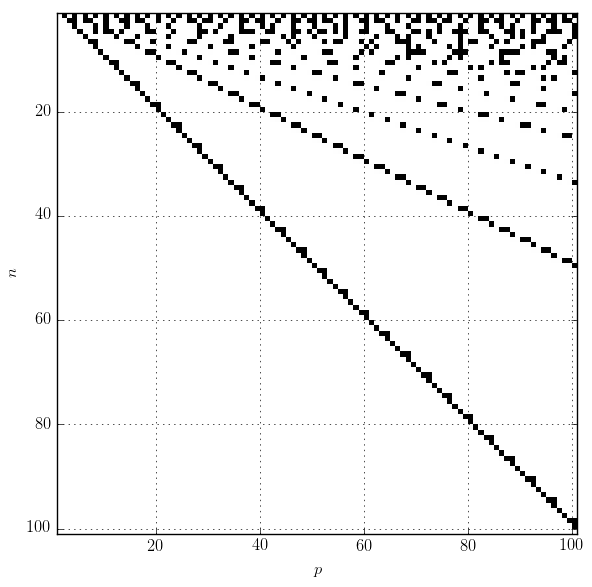
\includegraphics[width=0.6\textwidth]{./img/map_leg_100_100.png}
  \caption{Map of the extensions $E_p$ of Gauss-Legendre quadrature rules
           $P_n$ for $n \leq 100$ and $p$ up to $100$.}
  \label{fig:map_leg_100_100}
\end{figure}

\begin{figure}
  \centering
  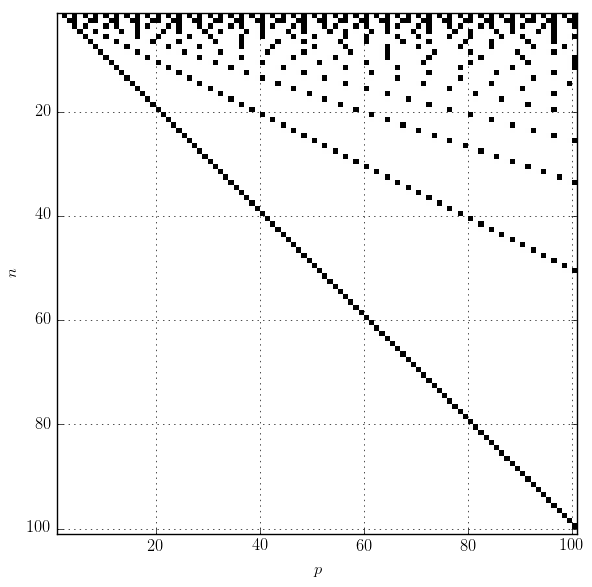
\includegraphics[width=0.6\textwidth]{./img/map_chebt_100_100.png}
  \caption{Map of the extensions $E_p$ of Gauss-Chebyshev quadrature rules
           $T_n$ for $n \leq 100$ and $p$ up to $100$.}
  \label{fig:map_chebt_50_50}
\end{figure}

\begin{figure}
  \centering
  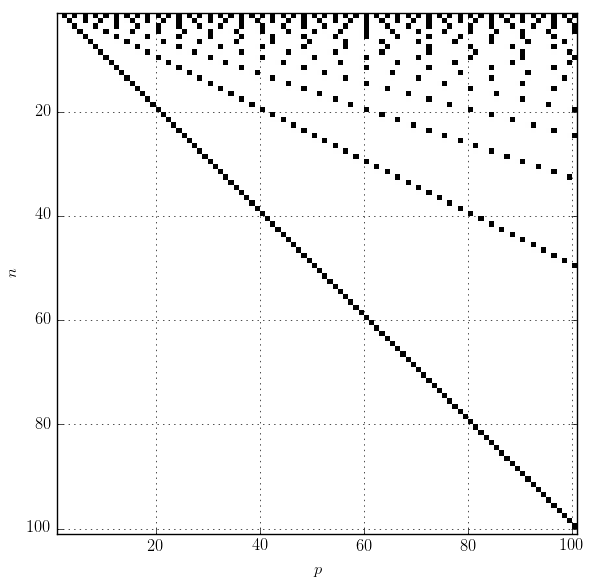
\includegraphics[width=0.6\textwidth]{./img/map_chebu_100_100.png}
  \caption{Map of the extensions $E_p$ of Gauss-Chebyshev quadrature rules
           $U_n$ for $n \leq 100$ and $p$ up to $100$.}
  \label{fig:map_chebu_100_100}
\end{figure}

For Laguerre polynomials there are no classical Kronrod extensions with $p = n+1$
at all. Higher order extensions are very sparse too, we could not find extensions
for any $12 < n \leq 100$ while keeping $p \leq 150$. There is no strong reason to
believe this would change if allowing for even higher $p$. Apart from that, such
rules would probably be of no practical use anyway.

\begin{figure}
  \centering
  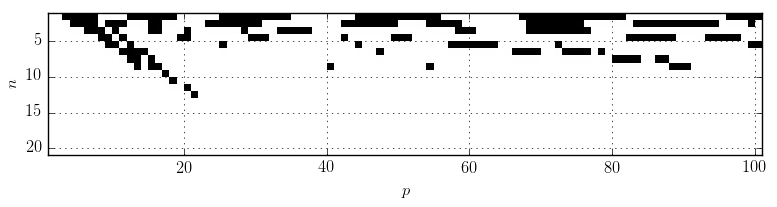
\includegraphics[width=0.8\textwidth]{./img/map_lag_20_100.png}
  \caption{Map of the extensions $E_p$ of Gauss-Laguerre quadrature rules
           $L_n$ for $n \leq 20$ and $p$ up to $100$. The part from
           $20 < n \leq 100$ not shown here does not contain any single
           valid extension. Compare also to Table 1 in \cite{kahaner_waldvogel_fullerton}.
           }
  \label{fig:map_lag_20_100}
\end{figure}

In the case of Hermite polynomials our computation indeed reveals the three possible
classical Kronrod rules for $n=1, p=2$ and $n = 2, p = 3$ and $n = 4, p = 5$. This
can be seen in the very top left corner of Figure \ref{fig:map_herm_50_100} and is
in perfect agreement with the literature \cite{monegato1976, kahaner-monegato, vladislav}.
In fact if we examine the three rules more closely, we will find that the case
$n = 4, p = 5$ does not have positive weights and is in turn ruled out by the
authors of the aforementioned papers.

\begin{figure}
  \centering
  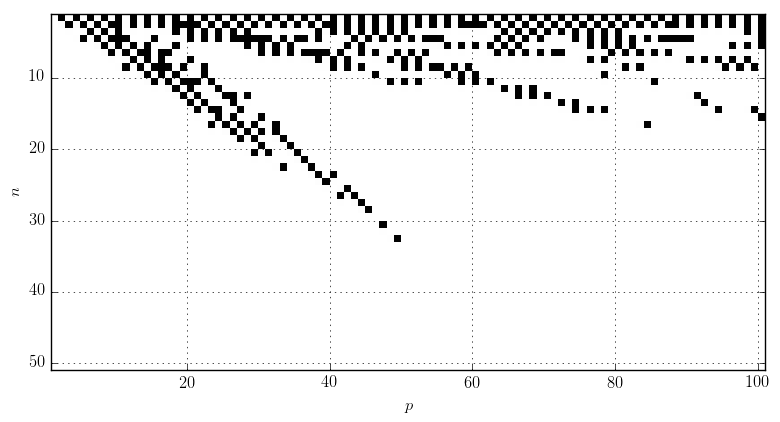
\includegraphics[width=0.8\textwidth]{./img/map_herm_50_100.png}
  \caption{Map of the extensions $E_p$ of Gauss-Hermite quadrature rules
           $H_n$ for $n \leq 50$ and $p$ up to $100$. The part from
           $50 < n \leq 100$ not shown here does not contain any single
           valid extension.}
  \label{fig:map_herm_50_100}
\end{figure}


\FloatBarrier
\section{Recursive Enumeration of nested Extensions}


In the last section we computed a single extensions $E_p$ over a
given rule $P_n$. This is enough in case of adaptive quadrature where all one
wants is to make an error estimate of the Gaussian quadrature by evaluation
of another quadrature rule having higher order. In that case the property of
nested nodes $\{\gamma_i\}_{i=1}^n \subset \{\gamma_i\}_{i=1}^{n+p}$ can reduce
computation cost.

The construction of quadrature rules for higher dimensional integrals
needs more than that. For the number of dimensions in the range from $4$ up
to some ten such quadrature rules can be done efficiently by the well known
Smolyak construction.

Given an initial polynomial $P_n$ of degree $n$, we want to find the set of all
extension towers\footnote{By abuse of notation, let $E_{p_k}$ denote the polynomial
of degree $p_k$ as well as the abstract extension over $E_{p_{k-1}}$ defined by it.}
%$P_n \subset E_{p_1} \subset E_{p_2} \subset \ldots \subset E_{p_k}$
$P_n \equiv E_{p_0} \subset E_{p_1} \subset \ldots \subset E_{p_k} \subset \ldots \subset E_{p_{k_{\textrm{max}}}}$
%$P = P_0 \subset P_1 \subset \ldots \subset P_k \subset \ldots \subset P_{k_{\textrm{max}}}$
over $P_n$ having finite height $k_{\textrm{max}}$. Additionally, we truncate this
potentially infinite set by requiring that the degrees $p_k$ of all polynomials $E_{p_k}$
never exceed a fixed upper bound $p_{\textrm{max}}$. This will in turn give a finite tree
of nested extensions. In the end, we denote a single extension from this set
by $\mathcal{K} = (n, p_1, \ldots, p_{k_{\textrm{max}}}) \in \mathbb{N}^{{k_{\textrm{max}}}+1}$.

Given the polynomial $P_{k-1}(x) := \prod_{i=0}^{k-1} E_{p_i}(x)$ that defines the
lower part $E_{p_0} \subset \ldots \subset E_{p_{k-1}}$ of this tower,
we can call Algorithm \ref{alg:recursive_search} with $P_{k-1}$ to compute recursively the remaining
upper layers $k, \ldots, k_{\textrm{max}}$ as far as they exist. This algorithm will perform a
flat exhaustive search on layer $k$ and then call itself for the next layer $k+1$. To get this
process started, we make an initial call for $k=1$ with $P_{0} := P_n \equiv E_{p_0}$ as shown
in \ref{alg:exhaustive_recursive_search}.

\begin{algorithm}
  \caption{Recursive search for extensions over $P_{k-1}$ on layer $k$}
  \label{alg:recursive_search}
  \begin{algorithmic}
    \Procedure{RecursiveSearch}{$P_{k-1}$, $p_{\textrm{max}}$, $k$, $k_{\textrm{max}}$}
    \State {}
    \Comment Search for possible extensions of $P_{k-1}$ of order $p \leq p_{\textrm{max}}$
    \For{$p = 1, \ldots, p_{\textrm{max}}$}
      \State $E_p := \textsc{ComputeExtension}(P_{k-1}, p)$
      \If{$E_p \not\equiv 0$}
        \State $\mathrm{valid} := \textsc{ValidateRoots}(E_p)$
      \Else
        \State $\mathrm{valid} := \mathrm{false}$
      \EndIf
      \If{$\mathrm{valid} = \mathrm{true}$}
        \State {}
        \Comment Valid extension $E_p$ of order $p$ found for $P_{k-1}$ on layer $k$
        \State $p_k := p$
        \State $\mathcal{K} := (p_0, \ldots, p_{k-1}, p_k) \in \mathbb{N}^{k+1}$
        \State $\mathcal{R} := \mathcal{R} \cup \mathcal{K}$
        \If{$k < k_{\textrm{max}}$}
          \State {}
          \Comment Follow the recursion down, descending to new layer $k+1$
          \State $P_{k} := P_{k-1} E_p$
          \State $\textsc{RecursiveSearch}(P_{k}, p_{\textrm{max}}, k+1, k_{\textrm{max}})$
        \Else
          \State {}
          \Comment Maximum recursion depth reached, not descending
        \EndIf
      \Else
        \State {}
        \Comment No valid extension of order $p$ found for $P_{k-1}$ on layer $k$
      \EndIf
    \EndFor
    \State {}
    \Comment Maximal extension order $p_{\textrm{max}}$ reached, ascending
    \EndProcedure
  \end{algorithmic}
\end{algorithm}

\begin{algorithm}
  \caption{Exhaustive recursive search up to $p_{\textrm{max}}$ and $k_{\textrm{max}}$}
  \label{alg:exhaustive_recursive_search}
  \begin{algorithmic}
    \Procedure{ExhaustiveRecursiveSearch}{$P$, $p_{\textrm{max}}$, $k_{\textrm{max}}$}
      \State $\mathcal{R} := \{\}$
      \Comment Storage for all the rules $\mathcal{K}$ found
      \State $p_0 := \deg P$
      \State $\textsc{RecursiveSearch}(P, p_{\textrm{max}}, 1, k_{\textrm{max}})$
    \EndProcedure
  \end{algorithmic}
\end{algorithm}

We denote by $\mathcal{Q}[p_0, \ldots, p_k]$ the quadrature rule and explicitly
the nodes and weights that can be computed from the nested Kronrod extension
$\mathcal{K} = (p_0, \ldots, p_k)$. Of course $\mathcal{Q}[n]$ is simple the
original quadrature rule we started with. In all cases considered here this
will be a Gauss rule of order $n$ having $n$ points.

\begin{figure}
  \centering
  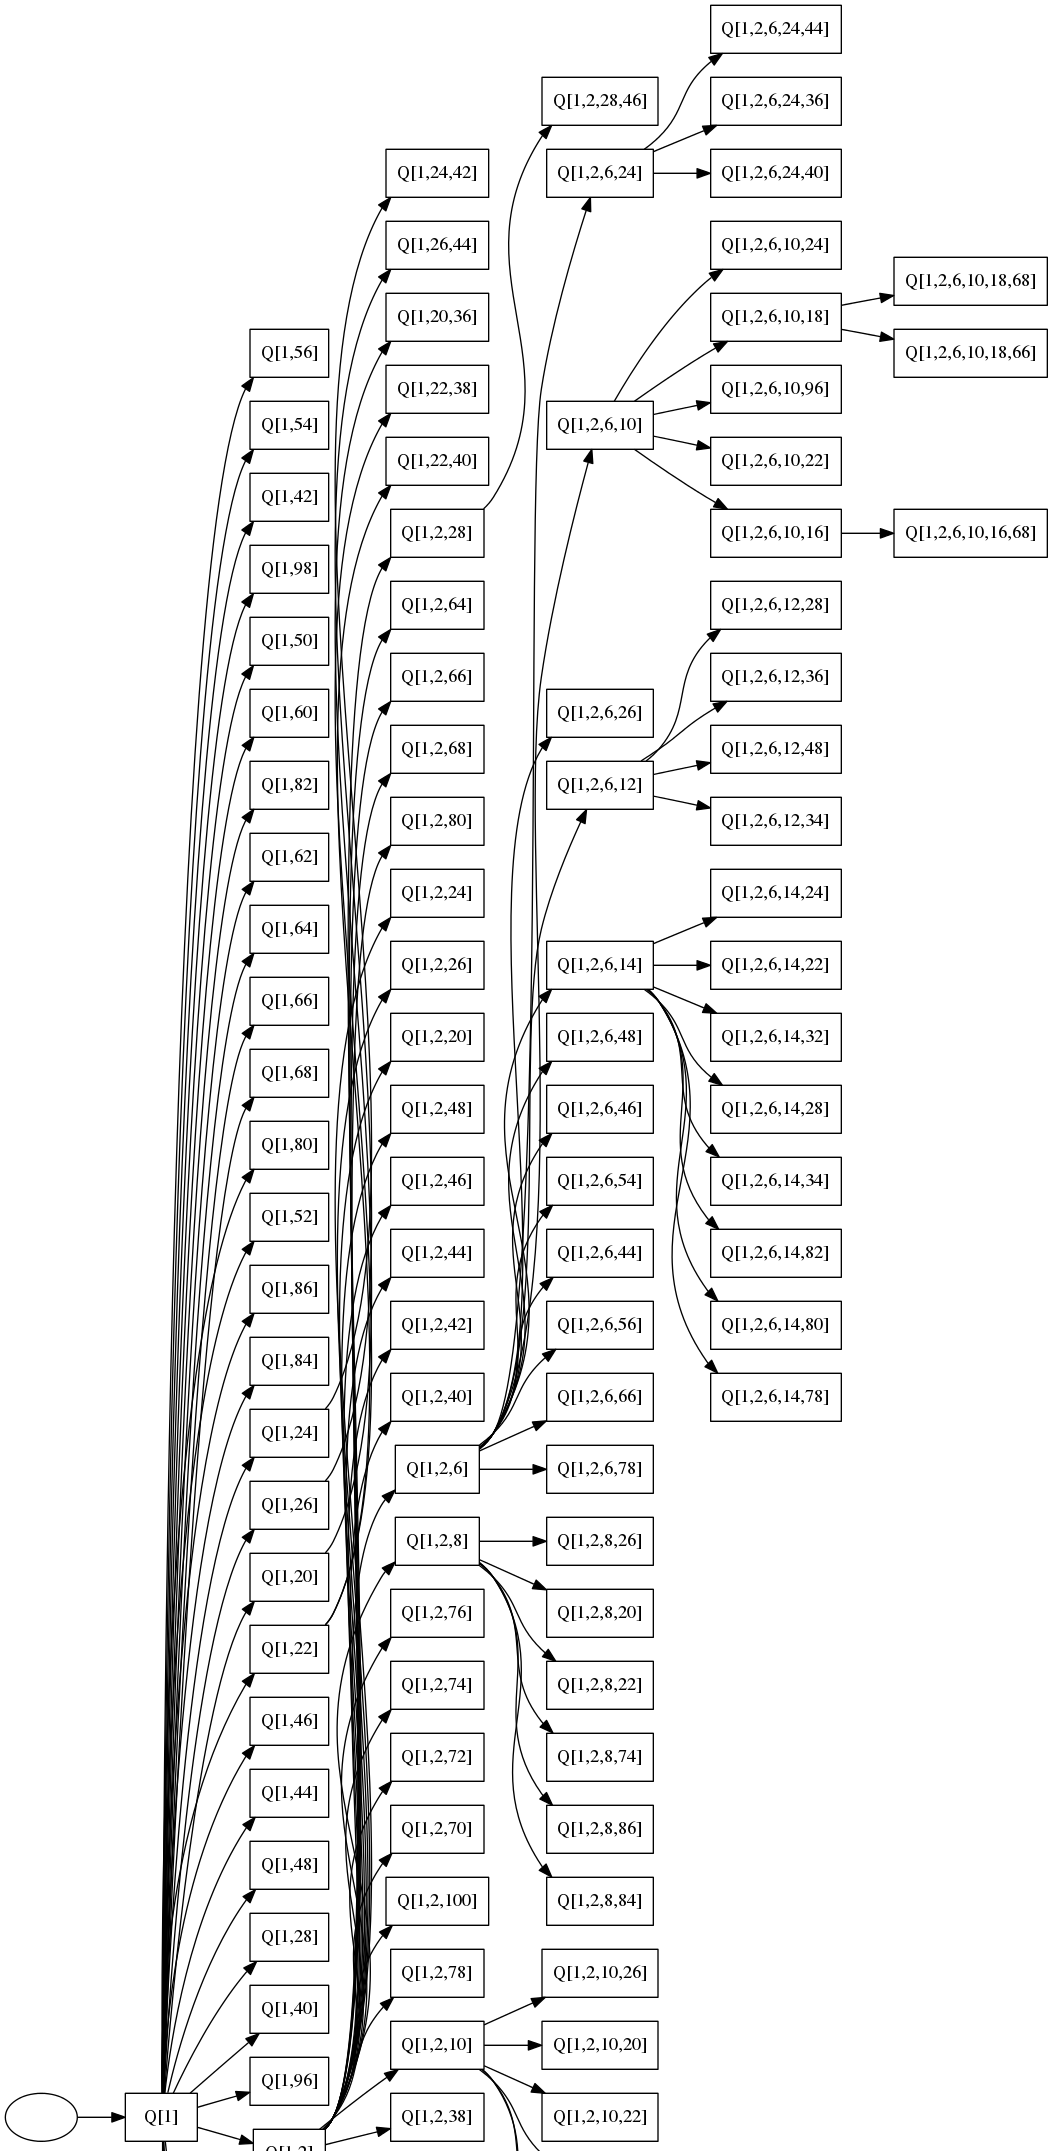
\includegraphics[width=0.8\linewidth]{./img/graph_hermite_1_100_6_part.png}
  \caption{Part of the tree of nested higher order Kronrod Extensions of the
  single point Gauss-Hermite rule $\mathcal{Q}[1]$.
  The new and for us most important rules are in the top right corner.}
  \label{fig:graph_1_100_6_part}
\end{figure}

If we run this algorithm for recursive enumeration, it finds a multitude
of higher order nested Kronrod extensions. Depending on the kind of orthogonal
polynomial we start with, there are large differences in the number and nesting
degree of the extensions. For polynomials which are specializations of the
Jacobi polynomials, we find the most regular structure which displays a vast number
of extensions. For other polynomials like the Laguerre polynomials there are almost
no extensions and the average nesting level is very low. From this large zoo of
possible $\mathcal{K}$ tuples, some of the more interesting ones are summarized
in the Tables \ref{tab:legendre_extensions}, \ref{tab:chebyshevt_extensions},
\ref{tab:chebyshevu_extensions}, \ref{tab:laguerre_extensions} and \ref{tab:hermite_extensions}
in appendix \ref{app:tables_extensions}.


\FloatBarrier
\section{Genz-Keister Multidimensional Construction}


Genz and Keister found an explicit construction by which efficient
special quadrature rules for an arbitrary number
of dimensions can be built. The resulting rules are
called \emph{fully-symmetric} for reasons that will become
clear later. In this section we review this construction of Genz
and Keister as given in \cite{genz, genz_keister}. We follow mostly their
development but focus mainly on the computational aspects and less
the theoretical derivation. Additionally we extend the construction
to Gauss-Chebyshev quadrature (both kinds) and analyze the resulting rules.


\subsection{The construction}

The quadrature rule $Q^{D,K}$ of \emph{level} $K \geq 0$ and
for use in $D$ dimensions is defined as:
\begin{equation} \label{eq:gk_basic_formula}
  \int_\Omega f(\vec{x}) \di{x} =:
  I[f] \approx Q^{D,K}[f]
       := \sum_{\mathbf{p} \in \mathcal{P}}
            f\left(\Gamma_{\mathbf{p}}\right)
            \omega_{\mathbf{p}}
\end{equation}
where $\mathcal{P}$ is the set of all integer partitions as defined below.
The node sets $\Gamma$ and weights $\omega$ are indexed by partitions
$\mathbf{p} \in \mathcal{P}$.
Define the set $\mathcal{P}$ of all admissible integer partitions
$\mathbf{p} := (\mathbf{p}_{1}, \ldots, \mathbf{p}_{D}) \in \mathbb{N}_{0}^{D}$
having $D$ parts (some of which can be zero) and $|\mathbf{p}| \leq K$
with $K \geq 0$ as:
\begin{equation} \label{eq:partition_set_def}
  \mathcal{P} :=
  \left\{
    \mathbf{p} \,
    \middle| K \geq \mathbf{p}_{1} \geq \cdots \geq \mathbf{p}_{D} \geq 0
    \wedge
    |\mathbf{p}| \leq K
  \right\}
  \,.
\end{equation}
A method for computing that set $\mathcal{P}$
is shown in Algorithm \ref{alg:ca_enumerate_integer_partitions}.
Before we look deeper into the details of this construction,
we need to introduce the set $\Lambda$ of so called \emph{generators}:
\begin{equation}
  \Lambda := \{\lambda_{0}, \lambda_{1}, \ldots, \lambda_{J}\}
\end{equation}
where we require that $\lambda_{0} \equiv 0$ and all $\lambda_{i}$ be
pair-wise distinct. There are obviously $J+1$ real non-negative generators.
A single quadrature point $\gamma \in \mathbb{R}^D$ is then an ordered
multiset of size $D$ of elements from $\Lambda$. Note that $\gamma$ is not
just a subset because elements are allowed to appear multiple times. The
specific items are then selected by an integer vector $\mathbf{k} \in \mathbb{N}_0^D$,
explicitly:
\begin{equation}
  \gamma_\mathbf{k} := \Lambda_\mathbf{k} = \left(\lambda_{k_1}, \ldots, \lambda_{k_D}\right) \,.
\end{equation}
We define $\delta$ as the number of components of $\gamma_\mathbf{k}$ that are 0.
As we require that only $\lambda_0$ is zero, $\delta$ is equivalent to the number
of zeros in $\mathbf{k}$.
Next we define the set $\overline{\gamma_\mathbf{k}}$ containing all
possible sign flips:
\begin{equation}
  \overline{\gamma_\mathbf{k}} \assign
  \sigma \gamma_\mathbf{k} =
  \{
  \left(\sigma_1 \gamma_1, \ldots, \sigma_D \lambda_D\right)
  \}_{\sigma \in \{-1,0,1\}^D}
\end{equation}
where $\sigma_d \in \{-1, 1\}$ or $\sigma_d = 0$ if and only if $\gamma_d = 0$.
The point $\gamma_\mathbf{k}$ gets mirrored into all $2^D$ orthants by $\sigma$.
Clearly, this set $\overline{\gamma_\mathbf{k}}$ is of size $2^{D-\delta}$ for
the reason that some points coincide with their own mirror images.

At this point we can go back and understand
the notation of equation \eqref{eq:gk_basic_formula}
where $\Gamma_\mathbf{p}$ stands for a whole set of nodes given by:
\begin{equation}
  \Gamma_\mathbf{p} \assign
  \bigcup_{\mathbf{q} \in \mathcal{S}_\mathbf{p}} \overline{\gamma_\mathbf{q}}
\end{equation}
and $\mathcal{S}_\mathbf{p}$ is the set of all permutations of the $D$
elements of $\mathbf{p} \in \mathcal{P}$. An algorithm for the enumeration
of all permutations is given in \ref{alg:ca_enumerate_permutations}.
Finally we find:
\begin{equation}
  f\left(\Gamma_\mathbf{p}\right) \assign
  \sum_{\mathbf{q} \in \mathcal{S}_p}
  \sum_{\gamma \in \overline{\gamma_\mathbf{q}}}
  f\left(\gamma_1, \ldots, \gamma_D\right) \,.
\end{equation}

What remains is the explanation of $\omega_\mathbf{p}$. The formula $(2.4)$
given in \cite{genz} looks quite simple but the efficient implementation needs
some care. For every admissible partition $\mathbf{p} \in \mathcal{P}$ the
corresponding weight can be computed by:
\begin{equation} \label{eq:gk_weight_def}
  \omega_{\mathbf{p}} := 2^{-(D-\delta)}
                         \sum_{|\mathbf{k}| \leq K - |\mathbf{p}|}
                         \prod_{d=1}^{D}
                           \frac{a_{\mathbf{k}_{d}+\mathbf{p}_{d}}}{P(\mathbf{k}_{d},\mathbf{p}_{d})}
\end{equation}
where we define the denominator:
\begin{equation} \label{eq:gk_weight_def_denom}
  P(\mathbf{k}_{d},\mathbf{p}_{d}) :=
  \prod_{\substack{i=0 \\
                   i\neq\mathbf{p}_{d}}}
       ^{\mathbf{k}_{d}+\mathbf{p}_{d}}
    \left( \lambda_{\mathbf{p}_{d}}^{2}-\lambda_{i}^{2} \right)
\end{equation}
and use the multi-index $\mathbf{k} \in \mathbb{N}_{0}^{D}$. Note that the
prefactor is exactly $1 / |\overline{\gamma_\mathbf{k}}|$.
Algorithm \ref{alg:ca_enumerate_lattice_points} implements a procedure
for enumeration of all relevant multi-indices.
This formula above presents us with several parts we need to compute.
Some of these parts can even be tabulated once for a maximal and
fixed $J$ value and independent of the dimension $D$.
Let us start with the numerator. There we need the value $a_i$ which
is defined by:
\begin{equation} \label{eq:gk_def_ai}
  a_{i} := \int_\Omega p_{i}(x) w(x) \di{x}, \quad i = 0, \ldots, J+1 \,,
\end{equation}
whereas the domain $\Omega$ and the weight function $w(x)$ are chosen
appropriately (see below). The polynomials $p_{i}(x)$ are defined as:
\begin{equation}
\begin{split}
  p_{0}(x) & := 1 \\
  p_{i}(x) & := \prod_{j=0}^{i-1} \left(x^{2} - \lambda_{j}^{2}\right)
\end{split}
\end{equation}
where the empty product equals 1. It holds that $\deg p_i = 2i$.
Since all the real numbers $\lambda_{j}$ are known, we can indeed
expand the product and write $p_i$ as $\sum_{j=0}^{2i} c_j x^j$
for some coefficients $c_j$. This enables us to compute the integral
in equation \eqref{eq:gk_def_ai} term-wise by using linearity:
\begin{equation}
  a_i = \sum_{j=0}^{2i} c_j \int_\Omega x^j w(x) \di{x} = \sum_{j=0}^{2i} c_j M_j
\end{equation}
where $M_j$ is the $j$-th moment and chosen according to Table
\eqref{eq:orthogonal_polynomials} and the explicit formulae shown thereafter.
For the Legendre, Chebyshev and Hermite case, the explicit formulae are
\eqref{eq:moments_legendre}, \eqref{eq:moments_chebyshevt}, \eqref{eq:moments_chebyshevt}
and \eqref{eq:moments_hermite_phy}.
Optionally, we can replace very small values by zero. As we will see later,
it is important to be able to decide whether $a_{i} = 0$. Because we
compute with real numbers (either floating point numbers or real ball arithmetic)
we can however never solve this problem exactly like in rational arithmetic.

\begin{algorithm}[h!]
  \caption{Compute table $\vec{A}$ of $a_{i}$ factors}
  \label{alg:gk_compute_a_values}
  \begin{algorithmic}
    \Procedure{ComputeAValues}{$\Lambda$, $\vec{M}$}
      \State $\vec{A} := \vec{0} \in \mathbb{R}^{J+1}$
      \State $p := 1$
      \For{$i=0, \ldots, J+1$}
        \State $a := 0$
        \For{$c_j$ in $\sum_{j=0}^{2i} c_j x^j = p$}
          \State $a := a + c_j \vec{M}_j$
        \EndFor
%         \For{$d = 0, \ldots, \deg p$}
%           \State $a := a + \textsc{Coefficient}(p, d) \, \vec{M}_d$
%         \EndFor
        \State $\vec{A}_i := a$
        \State $p := p \left(x^2 - \lambda_i^2\right)$
      \EndFor
    \EndProcedure
  \end{algorithmic}
\end{algorithm}

Computing the denominator as defined in \eqref{eq:gk_weight_def_denom}
is straight forward. Since we required the $\lambda_i$ to be pairwise
distinct this value never becomes zero and division poses no issue.

We notice that the product in formula \eqref{eq:gk_weight_def} only depends on
$\mathbf{p}_{d} =: \xi$ and the sum $\mathbf{p}_{d}+\mathbf{k}_{d} =: \eta$.
Therefore we can precompute a table of size $J+1 \times J+1$ indexed by $(\xi, \eta)$
whose entries are given by:
\begin{equation}
  \mat{T}_{\xi, \eta} := \frac{a_{\mathbf{k}_{d}+\mathbf{p}_{d}}}{P(\mathbf{k}_{d},\mathbf{p}_{d})} \,.
\end{equation}
In the example below, the top left corner of $\mat{T}$ is shown and we only
ever need the upper right triangular part:

\begin{center}
\begin{tabular}{|c|cccc|}
  \hline
  {}    & $\eta=0$ & $\eta=1$ & $\eta=2$ & $\eta=3$ \\
  \hline
  $\xi=0$ & $\frac{a_0}{1}$
          & $\frac{a_1}{(\lambda_0^2-\lambda_1^2)}$
          & $\frac{a_2}{(\lambda_0^2-\lambda_1^2)(\lambda_0^2-\lambda_2^2)}$
          & $\frac{a_3}{(\lambda_0^2-\lambda_1^2)(\lambda_0^2-\lambda_2^2)(\lambda_0^2-\lambda_3^2)}$ \\
  $\xi=1$ & 0
          & $\frac{a_1}{(\lambda_1^2-\lambda_0^2)}$
          & $\frac{a_2}{(\lambda_1^2-\lambda_0^2)(\lambda_1^2-\lambda_2^2)}$
          & $\frac{a_3}{(\lambda_1^2-\lambda_0^2)(\lambda_1^2-\lambda_2^2)(\lambda_1^2-\lambda_3^2)}$ \\
  $\xi=2$ & 0
          & 0
          & $\frac{a_2}{(\lambda_2^2-\lambda_0^2)(\lambda_2^2-\lambda_1^2)}$
          & $\frac{a_3}{(\lambda_2^2-\lambda_0^2)(\lambda_2^2-\lambda_1^2)(\lambda_2^2-\lambda_3^2)}$ \\
  $\xi=3$ & 0
          & 0
          & 0
          & $\frac{a_3}{(\lambda_3^2-\lambda_0^2)(\lambda_3^2-\lambda_1^2)(\lambda_3^2-\lambda_2^2)}$ \\
  \hline
\end{tabular}
\end{center}

Given the list $\Lambda$ of generators and all the values $a_{i}$ collected into
the list $\vec{A}$, we can compute the table $\mat{T}$ efficiently by Algorithm
\ref{alg:gk_compute_weight_factors}. By the use of this table, the implementation
of formula \eqref{eq:gk_weight_def} transforms into a series of trivial table
look-up steps. However, precomputation of $\mat{T}$ is expensive for larger $J$,
on the other hand it needs to be done only once for each $\Lambda$ and $w(x)$.
The numerator and denominator of the entries in $\mat{T}$ can become really large
numbers (remember that most moments include gamma functions), while their quotient
stays within reasonable range for floating point representation. For this reason
one can compute $\mat{T}$ to high precision with specialized software packages
like \texttt{flint} \cite{flint, Hart2010} and afterwards use these tabulated
values during usual floating point computations.

\begin{algorithm}[h!]
  \caption{Compute table $\mat{T}_{\xi,\eta}$ of weight factors}
  \label{alg:gk_compute_weight_factors}
  \begin{algorithmic}
    \Procedure{WeightFactors}{$\Lambda$, $\vec{A}$}
      \State $n := |\Lambda|$
      \State $\mat{T} \in \mathbb{R}^{n\times n}$
      \Comment Compute $T$ row by row
      \For{$\xi = 0, \ldots, n-1$}
        \State $t := 1$
        \For{$\eta = 0, \ldots, n-1$}
          \If{$\xi \neq \eta$}
            \State $t := t \left(\lambda_{\xi}^{2} - \lambda_{\eta}^{2}\right)$
          \EndIf
          \If{$\eta \geq \xi$}
            \State $\mat{T}_{\xi,\eta} := \frac{a_{\eta}}{t}$
          \EndIf
        \EndFor
      \EndFor
    \EndProcedure
  \end{algorithmic}
\end{algorithm}

At the end of the day we arrive at the following two Algorithms
\ref{alg:gk_compute_nodes} and \ref{alg:gk_compute_weights}
for computing the node set $\Gamma_\mathbf{p}$ and weights $\omega_\mathbf{p}$
for an arbitrary given partition $\mathbf{p} \in \mathcal{P}$.

\begin{algorithm}[h!]
  \caption{Compute nodes $\Gamma_\mathbf{p}$ for given $\mathbf{p} \in \mathcal{P} \subset \mathbb{N}_0^D$}
  \label{alg:gk_compute_nodes}
  \begin{algorithmic}
    \Procedure{Nodes}{$\mathbf{p}$, $\Lambda$}
      \State $\Gamma_\mathbf{p} := \{\}$
      \State $\delta := \textsc{NumberOfZeros}(\mathbf{p})$
      \State $\mathcal{S} := \textsc{Permutations}(D, \mathbf{p})$
      \For{$\mathbf{q} \in \mathcal{S}$}
        \For{$v = 0, \ldots, 2^{(D - \delta)}-1$}
          \State $u := 0$
          \For{$d = 0, \ldots, D-1$}
            \State $\gamma_d := \Lambda_{\mathbf{q}_d}$
            \If{$\mathbf{q}_d \neq 0$}
              \Comment Compute sign flip
              \If{$\lfloor\frac{v}{2^u}\rfloor \mod 2 = 1$}
                \State $\gamma_d := - \gamma_d$
              \EndIf
              \State $u := u + 1$
            \EndIf
          \EndFor
          \State $\Gamma_\mathbf{p} := \Gamma_\mathbf{p} \cup \gamma$
        \EndFor
      \EndFor
    \EndProcedure
  \end{algorithmic}
\end{algorithm}

\begin{algorithm}[h!]
  \caption{Compute weight $\omega_\mathbf{p}$ for given $\mathbf{p} \in \mathcal{P} \subset \mathbb{N}_0^D$}
  \label{alg:gk_compute_weights}
  \begin{algorithmic}
    \Procedure{Weights}{$\mathbf{p}$, $K$, $\mat{T}$}
      \State $\delta := \textsc{NumberOfZeros}(\mathbf{p})$
      \State $\omega_\mathbf{p} := 0$
      \State $\mathcal{L} := \textsc{EnumerateLatticePoints}(D, K - |\mathbf{p}|)$
      \For{$\mathbf{k} \in \mathcal{L}$}
        \State $w := 1$
        \For{$d = 0, \ldots, D-1$}
          \State $w := w \, \mat{T}_{\mathbf{p}_d, \mathbf{k}_d + \mathbf{p}_d}$
        \EndFor
        \State $\omega_\mathbf{p} := \omega_\mathbf{p} + w$
      \EndFor
      \State $\omega_\mathbf{p} := 2^{-(D-\delta)} \omega_\mathbf{p}$
    \EndProcedure
  \end{algorithmic}
\end{algorithm}

The last ingredient we need is the integer sequence $\vec{z} = (z_0, \ldots, z_J)$ defined as:
\begin{equation}
  \begin{split}
    z_0 & = 0 \\
    z_i & = l \quad \Leftrightarrow \quad a_{i+k} = 0 \quad \forall \, k = 0, \ldots, l-1 \,.
  \end{split}
\end{equation}

The reasoning behind this sequence and the specific definition summarizes to
the fact that we like to get many summands with $\omega_{\mathbf{p}} = 0$ in
equation \eqref{eq:gk_basic_formula}. Looking at the definition of the weights
in equation \eqref{eq:gk_weight_def} we have a sum-product structure. A single
product becomes zero if the numerator $a_{\mathbf{k}_d+\mathbf{p}_d} = 0$. This
then must happen for all summands in the sum. A simple algorithm to find $\vec{z}$
is given in \ref{alg:gk_compute_zsequence} below. It is limited in rigor because
of the zero test on floating point numbers.

\begin{algorithm}[h!]
  \caption{Compute the $\vec{z}$ sequence}
  \label{alg:gk_compute_zsequence}
  \begin{algorithmic}
    \Procedure{CompueZSequence}{$\vec{A}$}
      \State $\vec{z} := \vec{0} \in \mathbb{R}^{J+1}$
      \State $v := 0$
      \For{$i = 0, \ldots, J$}
        \If{$v = 0$}
          \While{$\vec{A}_{i+v} = 0$}
            \State $v := v + 1$
          \EndWhile
        \Else
          \State $v := v - 1$
        \EndIf
        \State $\vec{z}_i := v$
      \EndFor
    \EndProcedure
  \end{algorithmic}
\end{algorithm}

Finally, we cite theorem 3.1 from \cite{genz} but omit the proof:

\begin{theorem*}
  \label{th:zero_weights}
  A fully symmetric rule using a generator set $\Lambda$ has weights $\omega_{\mathbf{p}} = 0$
  if $|\mathbf{p}| + |\vec{z}(\mathbf{p})| > K$.
\end{theorem*}

This theorem tells us which partitions $\mathbf{p}$ we can omit when assembling
the quadrature rule. The full algorithm for the construction of fully symmetric quadrature
rules in $D$ dimensions and of level $K$ is shown in \ref{alg:gk_construction}.
The whole procedure is general in the sense that we can apply it to both the Legendre and
Hermite cases as it was already done in \cite{genz} and \cite{genz_keister} respectively.
Further we can repeat the very same computations for both kinds of Gauss-Chebyshev
quadrature which is new. As we have seen in the last section, there exists a plethora
of nested higher order Kronrod extensions for some orthogonal polynomials. Each of these
can serve as the basis $\mathcal{K}$ for the generator set $\Lambda$. Genz and Keister used in
the Hermite case the Kronrod extensions $\mathcal{K} = (1, 2, 6, 10, 16)$ and $\mathcal{K} = (1, 2, 8, 20)$.
One should note that not all rules are equally well suited. A criterion on the expected
\emph{sparsity} of the final rule is the number of zero elements in the $\vec{z}$ sequence.
The more non-zero elements the better, but unfortunately such sequences are rare.
Additionally there appears the question of stability which was discussed in \cite{genz}.
Novak and Ritter show in \cite{novak_ritter}, section 6, that the Genz-Keister construction
produces quadrature rules which are of classical Smolyak form. This is convenient
for two reasons. First, we can construct $D$ dimensional rules either by direct full
Genz-Keister construction or by Smolyak construction applied to the set of one-dimensional
Genz-Keister rules. Second, the convergence and error analysis from Smolyak theory is
also valid for this construction.

\begin{algorithm}[h!]
  \caption{Genz-Keister construction}
  \label{alg:gk_construction}
  \begin{algorithmic}
    \Procedure{GenzKeisterConstruction}{$D, K$}
      \State $\Gamma := \{\}$
      \Comment Nodes and weights as ordered sets
      \State $\Omega := \{\}$
      \State $ $
      \Comment Precompute fundamental tables
      \State $\Lambda := \textsc{ComputeGenerators}(\mathcal{K})$
      \State $\vec{M} := \textsc{ComputeMoments}()$
      \State $\vec{A} := \textsc{ComputeAValues}(\Lambda, \vec{M})$
      \State $\mat{T} := \textsc{WeightFactors}(\Lambda, \vec{A})$
      \State $ $
      \Comment Construct multi-dimensional rule
      \State $\mathcal{P} := \textsc{EnumeratePartitions}(D, K)$
      \For{$\mathbf{p} \in \mathcal{P}$}
        \If{$|\mathbf{p}| + |\vec{z}(\mathbf{p})| \leq K$}
          \State $\Gamma_\mathbf{p} := \textsc{Nodes}(\mathbf{p}, \Lambda)$
          \State $\omega_\mathbf{p} := \textsc{Weights}(\mathbf{p}, K, \mat{T})$
          \State $\Gamma := \Gamma \cup \Gamma_\mathbf{p}$
          \State $\Omega := \Omega \cup \omega_\mathbf{p}$
          \Comment Add $|\Gamma_\mathbf{p}|$ times the weight $\omega_\mathbf{p}$
        \EndIf
      \EndFor
    \EndProcedure
  \end{algorithmic}
\end{algorithm}


\subsubsection{Combinatorial Algorithms}


In this section we summarize the combinatorial algorithms that
can be used during the Genz-Keister construction. In the programming
language \texttt{python} they can be implemented very efficiently by
the use of \texttt{yield} statements inside so called \emph{generator expressions}.

The Algorithm \ref{alg:ca_enumerate_integer_partitions} can
be used for enumeration of the set $\mathcal{P}$ defined in
\eqref{eq:partition_set_def}. This works for any given value
of $D \geq 1$ and maximal element size $K \geq 0$. The elements
$\mathbf{p} \in \mathcal{P}$ will be generated by increasing value
of $|\mathbf{p}|$ until the boundary $K$ is hit.

\begin{algorithm}[h!]
  \caption{Enumerate the set $\mathcal{P}$ of all integer partitions}
  \label{alg:ca_enumerate_integer_partitions}
  \begin{algorithmic}
    \Procedure{EnumeratePartitions}{$D$, $K$}
      \State $\mathcal{P} := \{\}$
      \State $\mathbf{p} := \vec{0} \in \mathbb{N}_{0}^{D}$
      \While{$|\mathbf{p}| \leq K$}
        \State $\tau := \mathrm{false}$
        \State $p := \mathbf{p}_{0}$
        \For{i = 1, \ldots D-1}
          \State $p := p + \mathbf{p}_i$
          \If{$\mathbf{p}_{0} \leq \mathbf{p}_{i} + 1$}
            \State $\mathbf{p}_{i} := 0$
          \Else
            \State $\mathbf{p}_{0} := p - i (\mathbf{p}_{i} + 1)$
            \For{j = 1, \ldots, i}
              \State $\mathbf{p}_{j} := \mathbf{p}_{i} + 1$
            \EndFor
            \State $\mathcal{P} := \mathcal{P} \cup \mathbf{p}$
            \State $\tau := \mathrm{true}$
            \State \bf{break}
          \EndIf
        \EndFor
        \If{$\tau = \mathrm{false}$}
          \State{$\mathbf{p}_{0} := p + 1$}
          \If{$|\mathbf{p}| \leq K$}
            \State $\mathcal{P} := \mathcal{P} \cup \mathbf{p}$
          \EndIf
        \EndIf
      \EndWhile
    \EndProcedure
  \end{algorithmic}
\end{algorithm}

An algorithm to enumerate the set $\mathcal{S}$ of all entry-wise
permutations of a given vector $\mathbf{p} \in \mathbb{N}_{0}^{D}$
is shown next in \ref{alg:ca_enumerate_permutations}. This algorithm
will generate the permutations in reverse lexicographic order,
starting with $\mathbf{p}$.

\begin{algorithm}[h!]
  \caption{Enumerate the set $\mathcal{S}$ of all permutations
    of the entries of $\mathbf{p} \in \mathbb{N}_{0}^{D}$}
  \label{alg:ca_enumerate_permutations}
  \begin{algorithmic}
    \Procedure{Permutations}{$D$, $\mathbf{p}$}
      \State $\mathcal{S} := \{\mathbf{p}\}$
      \State $\tau := \mathrm{true}$
      \While{$\tau = \mathrm{true}$}
        \State $\tau := \mathrm{false}$
        \For{$i = 1, \ldots, D-1$}
          \State $p := \mathbf{p}_{i}$
          \If{$\mathbf{p}_{i-1} > p$}
            \State $I := i$
            \If{$i > 1$}
              \State $J := I$
              \For{$j = 0, \ldots, \lfloor \frac{I}{2} \rfloor -1 $}
                \State $q := \mathbf{p}_{j}$
                \If{$q \leq p$}
                  \State $I := I - 1$
                \EndIf
                \State $\mathbf{p}_{j} := \mathbf{p}_{i-j-1}$
                \State $\mathbf{p}_{i-j-1} := q$
                \If{$\mathbf{p}_{j} > p$}
                  \State $J := j + 1$
                \EndIf
              \EndFor
              \If{$\mathbf{p}_{I-1} \leq p$}
                \State $I := J$
              \EndIf
            \EndIf
            \State $\mathbf{p}_{i} := \mathbf{p}_{I-1}$
            \State $\mathbf{p}_{I-1} := p$
            \State $\mathcal{S} := \mathcal{S} \cup \mathbf{p}$
            \State $\tau := \mathrm{true}$
            \State \bf{break}
          \EndIf
        \EndFor
      \EndWhile
    \EndProcedure
  \end{algorithmic}
\end{algorithm}

In the definition of the weights in formula \eqref{eq:gk_weight_def}
we need to iterate over the set $\mathcal{L} := \{\mathbf{k_{i}}\}$ of all
lattice points $\mathbf{k} \in \mathbb{N}_{0}^{D}$ up to some maximal value of
the $l_{1}$ norm. The Algorithm \ref{alg:ca_enumerate_lattice_points}
shows an efficient method for the enumeration of all such points. It
is well known that the cardinality of $\mathcal{L}$ is:
\begin{equation}
  |\mathcal{L}| = \left(\frac{K+1}{D}\right) \binom{D+K}{K+1} \,.
\end{equation}
For more details see for example \cite{serra-sagrista}.

\begin{algorithm}[h!]
  \caption{Enumerate lattice points in $\{\mathbf{k_{i}}\} =: \mathcal{L} \subset \mathbb{N}_{0}^{D}$
    with $\|\mathbf{k_{i}}\|_{1} \leq N$}
  \label{alg:ca_enumerate_lattice_points}
  \begin{algorithmic}
    \Procedure{EnumerateLatticePoints}{$D$, $N$}
      \State $\mathcal{L} := \{\} $
      \For{$n = 0, \ldots, N$}
        \State $\mathbf{k} := \vec{0} \in \mathbb{N}_{0}^{D}$
        \State $\mathbf{k}_{0} := n$
        \State $\mathcal{L} := \mathcal{L} \cup \mathbf{k}$
        \State $c := 1$
        \While{$\mathbf{k}_{D-1} < n$}
          \If{$c = D$}
            \For{$i = c-1, \ldots, 1$}
              \State $c := i$
              \If{$\mathbf{k}_{i-1} \neq 0$}
                \State \bf{break}
              \EndIf
            \EndFor
            \State $\mathbf{k}_{c-1} := \mathbf{k}_{c-1} - 1$
            \State $c := c +1$
            \State $\mathbf{k}_{c-1} := n$
            \For{$i = 0, \ldots, c-2$}
              \State $\mathbf{k}_{c-1} := \mathbf{k}_{c-1} - \mathbf{k}_{i}$
            \EndFor
            \If{$c < D$}
              \For{$i = c, \ldots, D-1$}
                \State $\mathbf{k}_{i} := 0$
              \EndFor
            \EndIf
            \State $\mathcal{L} := \mathcal{L} \cup \mathbf{k}$
          \EndIf
        \EndWhile
      \EndFor
    \EndProcedure
  \end{algorithmic}
\end{algorithm}


\FloatBarrier
\section{Nested Rules for Orthogonal Polynomials}

In this section we present various results for the classical orthogonal polynomials
and related Gauss quadrature schemes. For each scheme we could find at least one
replacement having nested nodes based on the Genz-Keister construction.

The generator set $\Lambda$ is in each case obtained by recursive higher order
Kronrod extensions $\mathcal{K} := (k_1, \ldots, k_p)$. For each extension level $k_i$
we then get a subset of nodes $\{\lambda_{i_1}, \ldots, \lambda_{i_q}\}$ from the corresponding
polynomial $E_{k_i}$. The final rule now depends on the ordering of these generators
and different orderings can lead to a non-negligible difference in overall stability. Permutation of
the nodes $\lambda_{i_j}$ within each subset does not change the number of function evaluations
required. The original authors came up with the following heuristic for sorting the
generators: begin each subset with its largest generator and then alternate the remaining
generators always using extremal values. They claim that this procedure yields
rules with a good (but not necessarily optimal) stability factor. In our notation
this factor reads:
\begin{equation*}
  C \assign \sum_{\mathbf{p} \in \mathcal{P}} N_{\mathbf{p}} |\omega_{\mathbf{p}}|
\end{equation*}
where for any partition $\mathbf{p}$ with $n$ distinct parts $\mathbf{p}_j$ each
having multiplicity $m_j$ the value $N_{\mathbf{p}}$ is given by:
\begin{equation*}
  N_{\mathbf{p}} = \frac{2^{|m|} D!}
                        {(D-|m|)! \, m_1! \cdots m_n!} \,.
\end{equation*}
In principle one could test all permutations of the generators and search for
one minimizing this stability constant. We will choose this alternating ordering
as default.
The order of a quadrature rule $Q^K$ is given by theorem 2.1 in \cite{genz}
and shown to be:
\begin{equation} \label{eq:gk_rul_order}
  2 K + 1 \,.
\end{equation}
The $K$ in this formula is, for each fixed quadrature
rule, the maximal value of $K$ for which the Genz-Keister construction results
in the given rule. For example in the Hermite case $K=9, \ldots, 14$ all yield
the same node-weight pairs. The order os this rule is then $2\cdot 14 + 1 = 29$.

Lemma 4.1 in \cite{holtz} gives conditions on the one-dimensional rules
such that the Smolyak construction of level $K$ from these rules has
order at least $2K-1$. It can be seen from Figures \ref{fig:number_nodes_legendre},
\ref{fig:number_nodes_chebyshevt}, \ref{fig:number_nodes_chebyshevu} and
\ref{fig:number_nodes_hermitephy} that the rules discussed here fulfill the
required conditions as their orders are always large enough.

% Finally, corollary 7 from \cite{novak_ritter} gives the degree of exactness
% for $K \geq D - 1$ as $2 (K+1-D) + 1$.
% \marginpar{TODO: inconsistent?}

\subsection{Legendre Quadrature}

For the Legendre polynomials $P_n$ we can find various Kronrod extensions. The
most suitable one seems to be $\mathcal{K} = (1,2,4,8,16,32)$. The Genz-Keister
construction built upon this set of generators has the following $\vec{z}$
sequence:
\begin{equation*}
  \vec{z} = (0, 0, 1, 0, 2, 1, 0, 0, 4, 3, 2, 1, 0, 0, 0, 0, 11, 10, 9, 8, 7, 6, 5, 4, 3, 2, 1, 0, 5, 4, 3, 2, 1)
\end{equation*}
where a large number of non-zero elements occur. Also we can in principle
arbitrarily extend $\mathcal{K}$ by doubling the degree. If we use this
extension we get the one-dimensional quadrature nodes and weights shown
in Figure \ref{fig:gk_legendre_nodes_1d}. For most values of the level $K$
the weights behave well but for some they start oscillating and even become
negative. These special values of $K$ correlate with extra zeros in the
$\vec{z}$ sequence. Figure \ref{fig:gk_legendre_nodes_2d} shows the sparse
node distribution in the plane for two-dimensional quadrature rules.
Notice that for $D < 3$, using the Genz-Keister construction results
in more quadrature points than the full tensor product Ansatz. This
fact is examined in Figures \ref{fig:gk_legendre_ratio} and \ref{fig:gk_legendre_ratio_large}.

\begin{figure}[h]
  \centering
  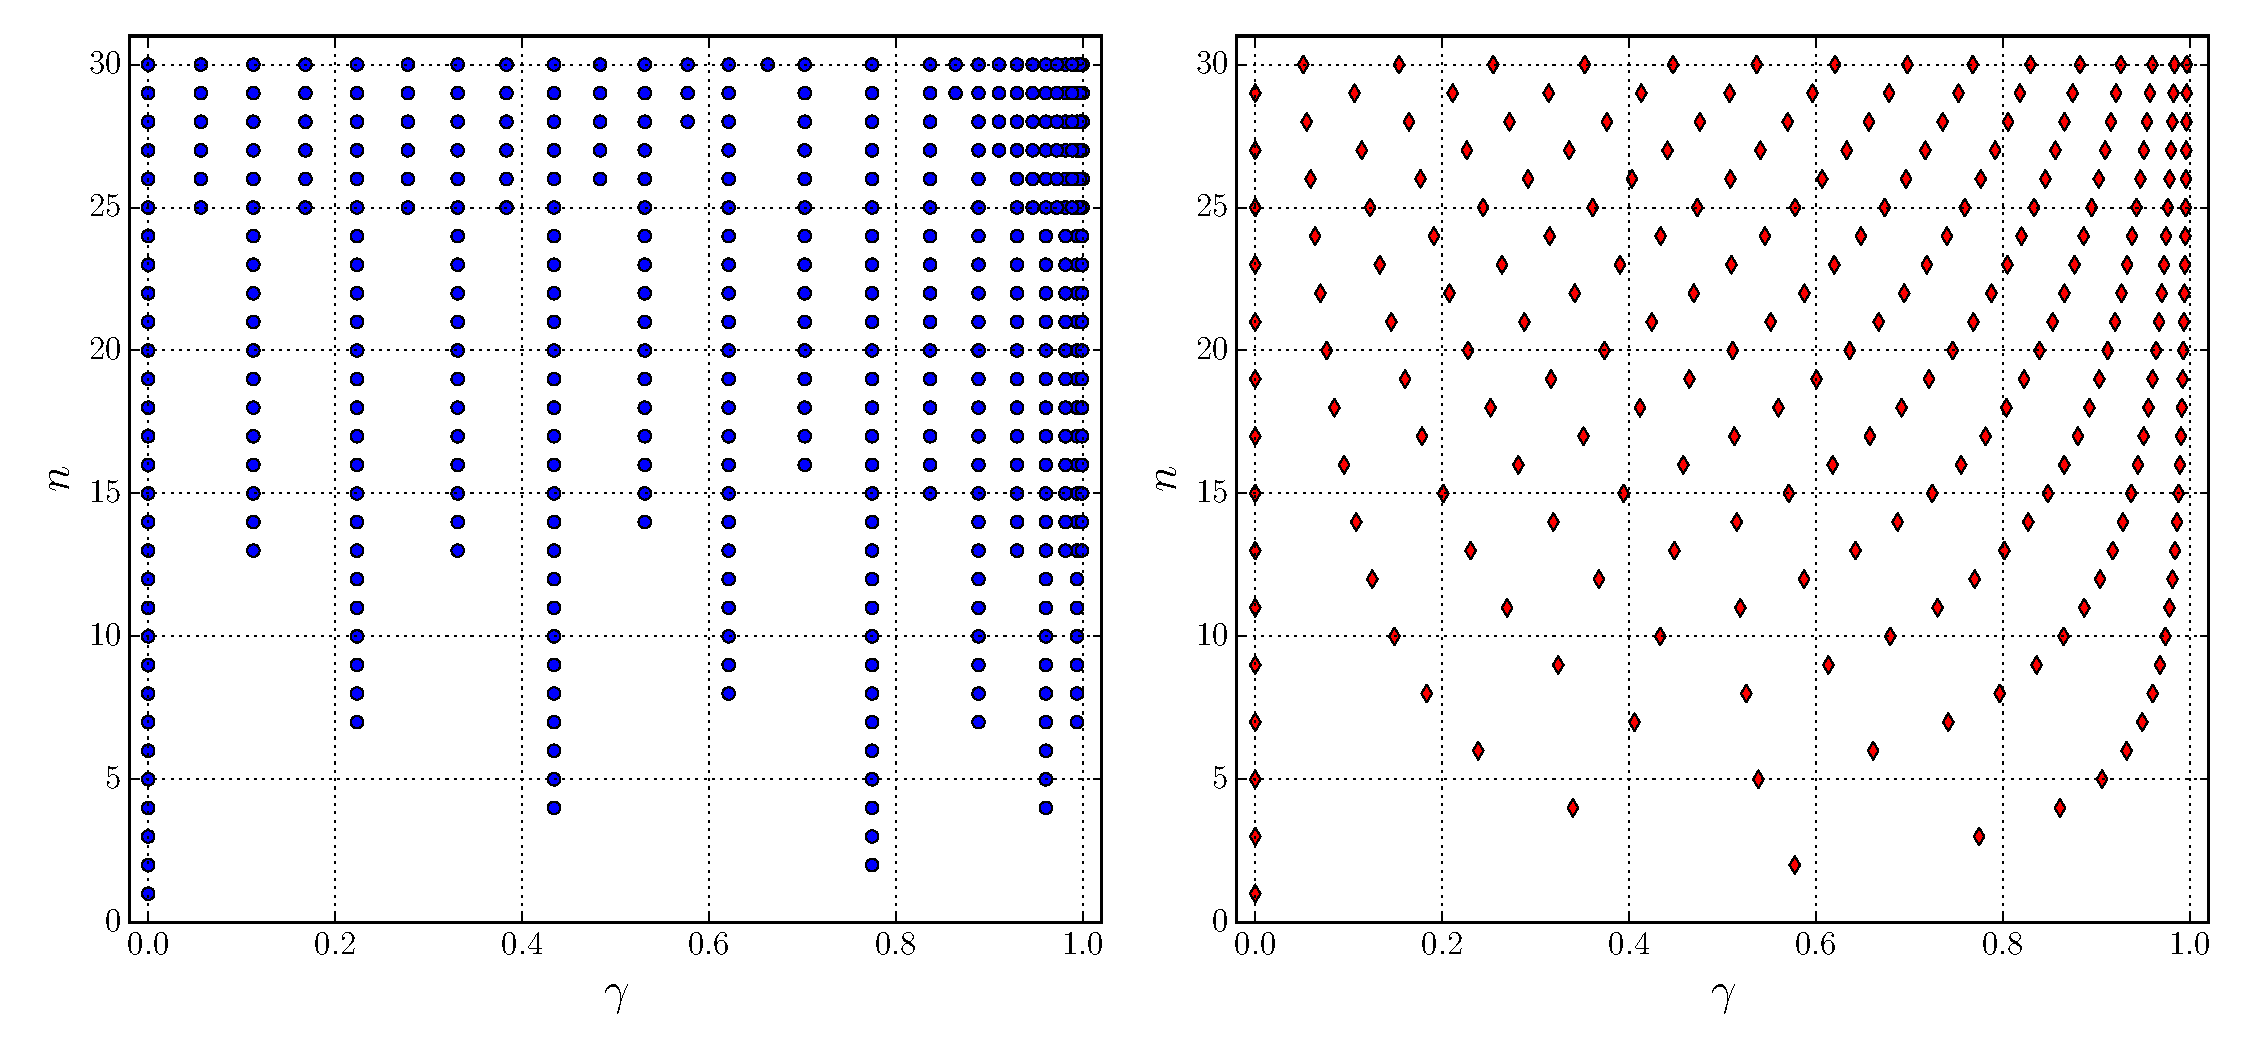
\includegraphics[width=\linewidth]{./img/gk_legendre_nodes_cmp.pdf}
  \caption{Comparison of Gauss-Legendre nodes (right) and nested Genz-Keister nodes (left)
  based on the $\mathcal{K} = (1,2,4,8,16,32)$ Kronrod extension. The points are
  nicely nested and well suited for sparse grids.}
  \label{fig:gk_legendre_nodes_cmp}
\end{figure}

\begin{figure}
  \centering
  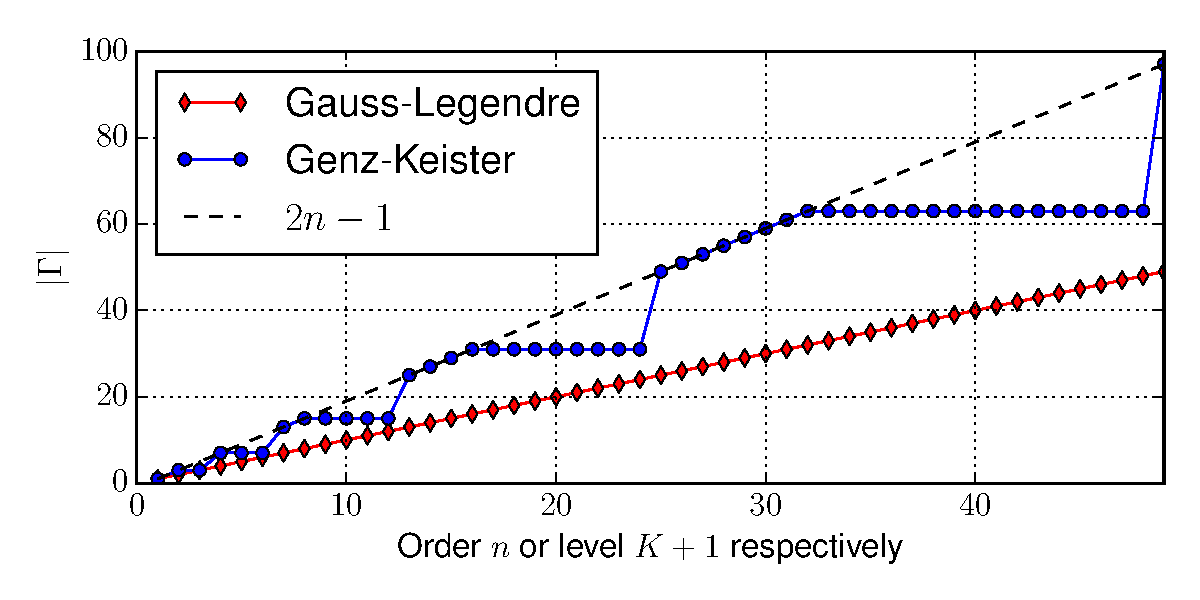
\includegraphics[width=\linewidth]{./img/number_nodes_legendre.pdf}
  \caption{Number of nodes for the one-dimensional Gauss-Legendre and Genz-Keister quadrature
  rules of order $n$ or level $K$ respectively.}
  \label{fig:number_nodes_legendre}
\end{figure}

\begin{figure}
  \centering
  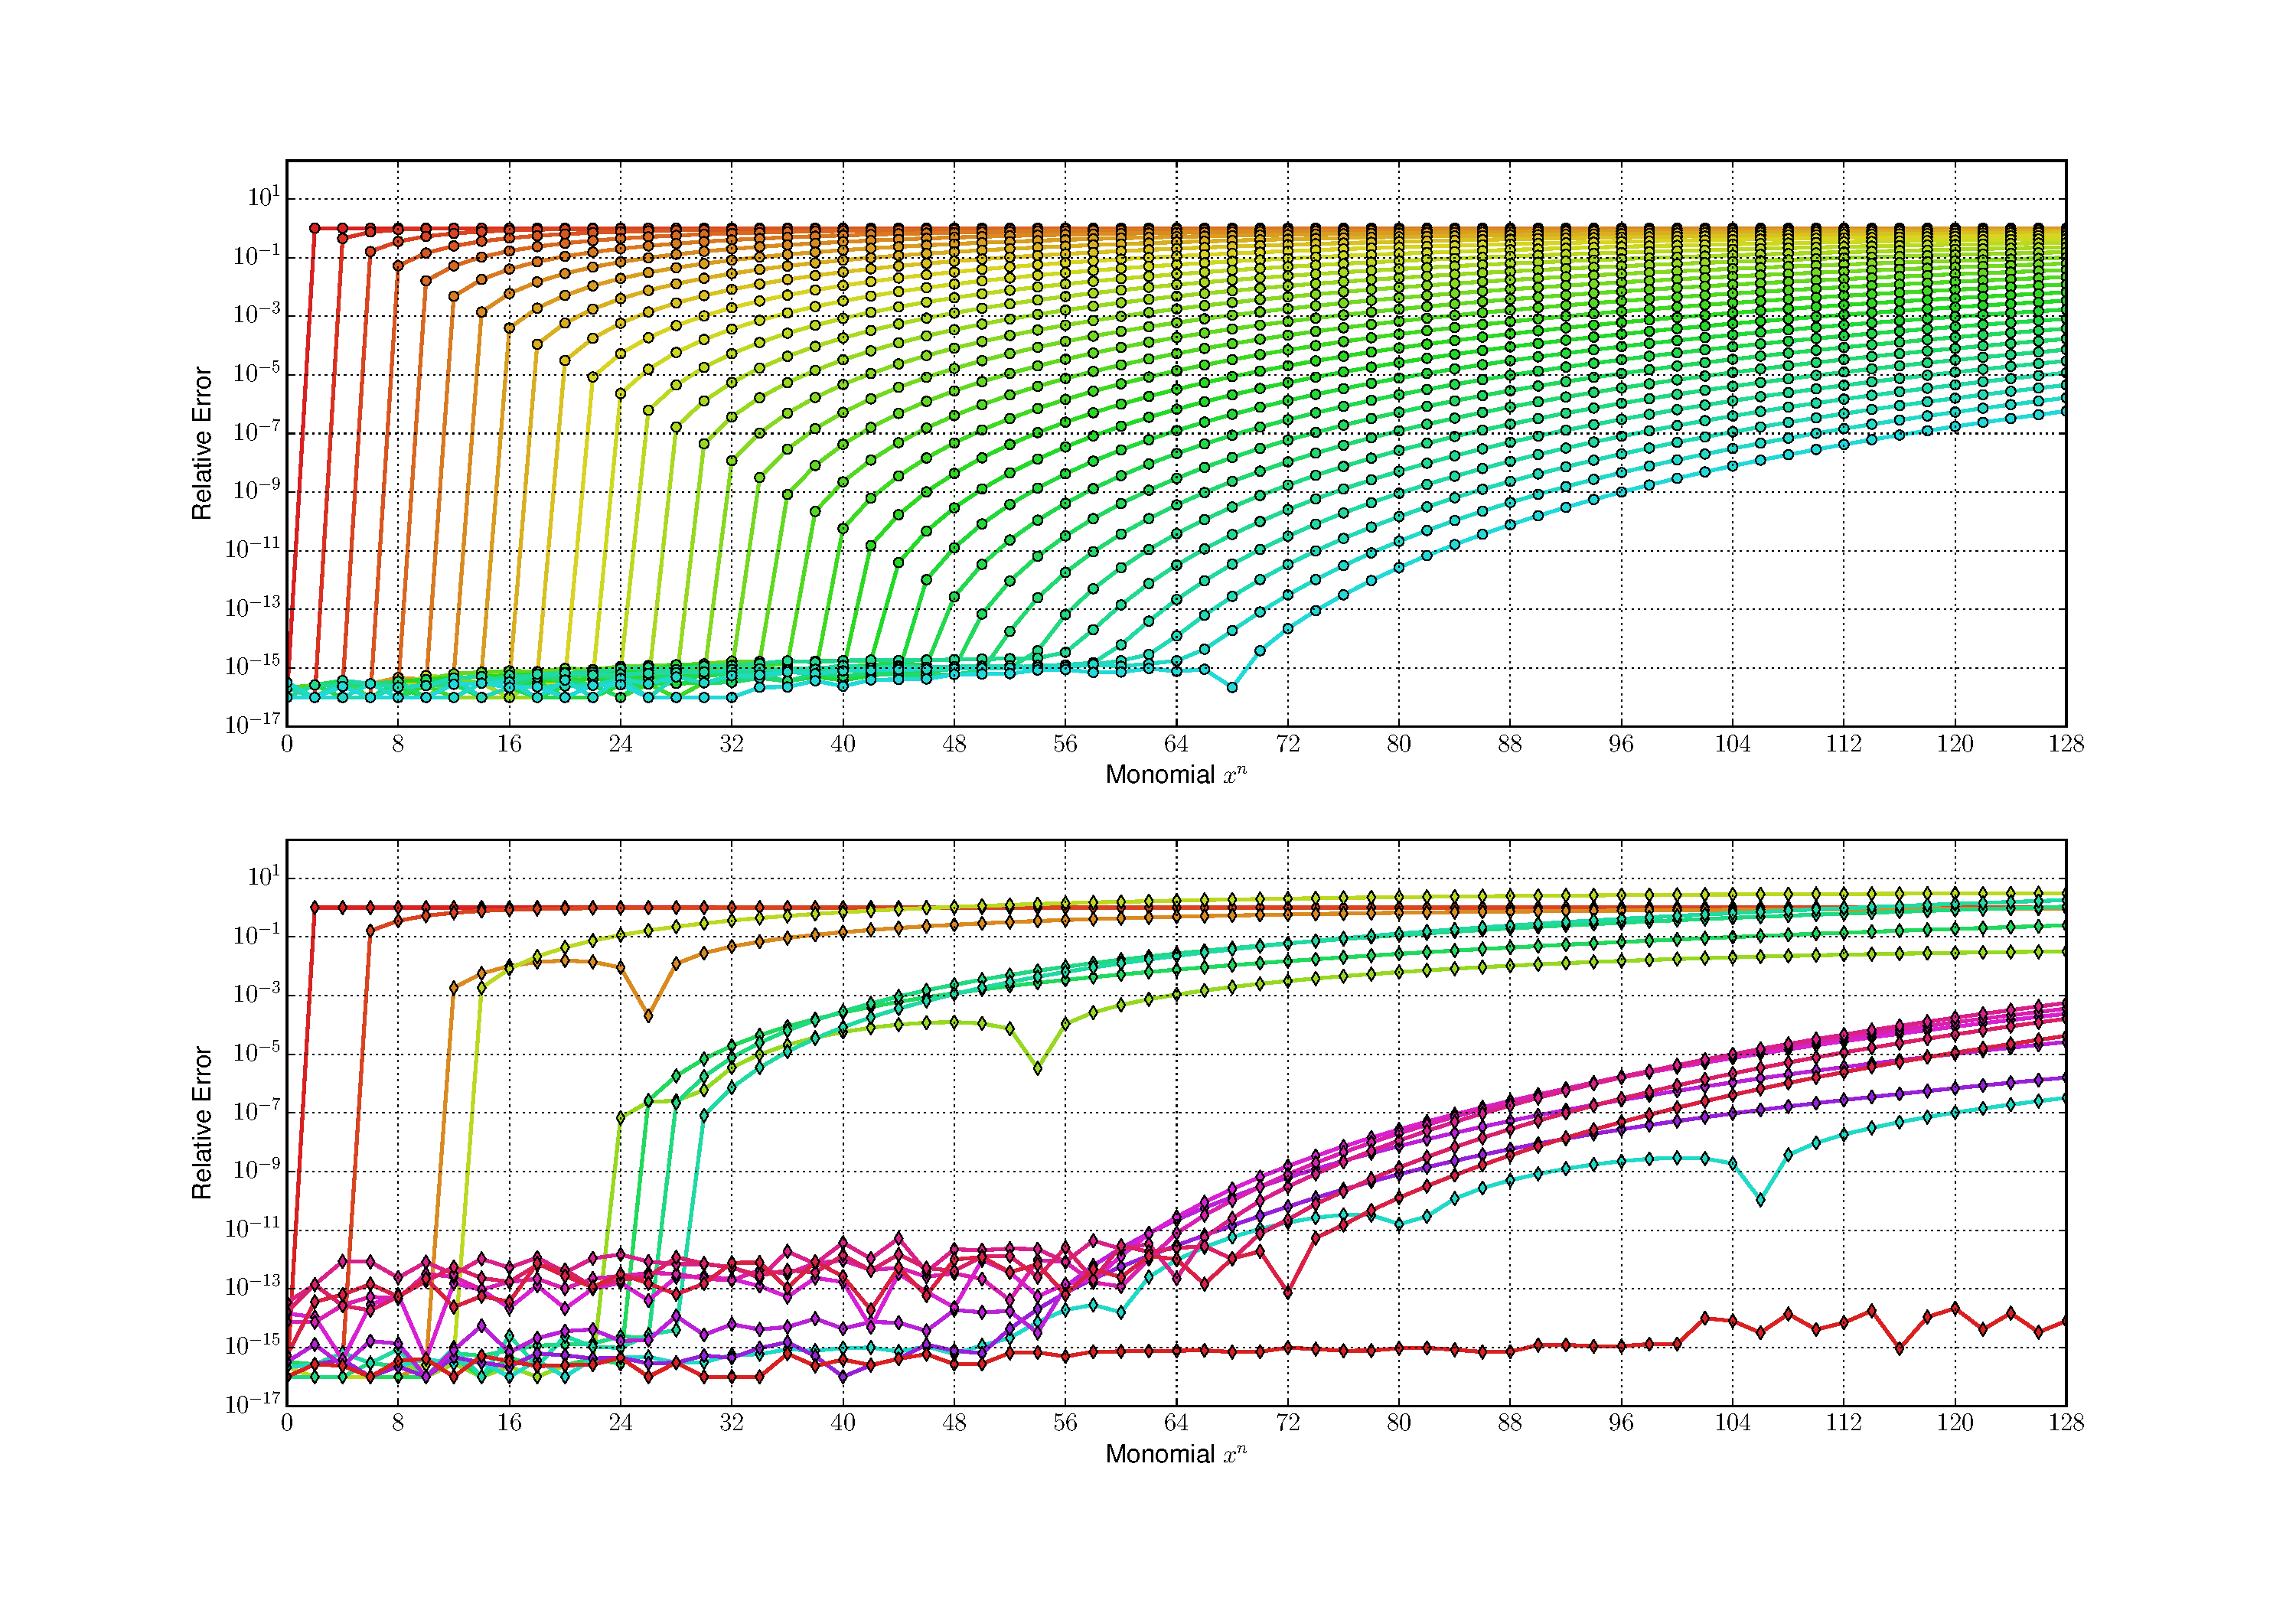
\includegraphics[width=\linewidth]{./img/monomial_errors_legendre.pdf}
  \caption{Relative quadrature error for integration of single univariate monomials $x^n$ of increasing degree $n$.
  Each line represents a quadrature rule and the color indicates the number of nodes (colors wrap around once though).
  The upper plot shows Gauss-Legendre rules as reference while the lower one shows the Genz-Keister rules.
  The number of nodes for each of these rules is:
  $1$, $3$,  $7$, $13$, $15$, $25$, $27$, $29$, $31$, $49$, $51$, $53$, $55$, $57$, $59$, $61$, $63$
  and the orders according to \eqref{eq:gk_rul_order} are:
  $1$, $5$, $11$, $13$, $23$, $25$, $27$, $29$, $47$, $49$, $51$, $53$, $55$, $57$, $59$, $61$, $95$
  which perfectly agrees with the figure.
  Starting with the $31$ point rule, the rules become somewhat unstable
  and do not reach the machine epsilon error level. This can be explained
  by growing oscillations in the weights for some of the rules. (Refer to Figure
  \ref{fig:gk_legendre_nodes_1d} though the rules affected are beyond the range
  of that plot.) The rule having $63$ nodes is very stable again.}
  \label{fig:monomial_errors_legendre}
\end{figure}

\begin{figure}[h]
  \centering
  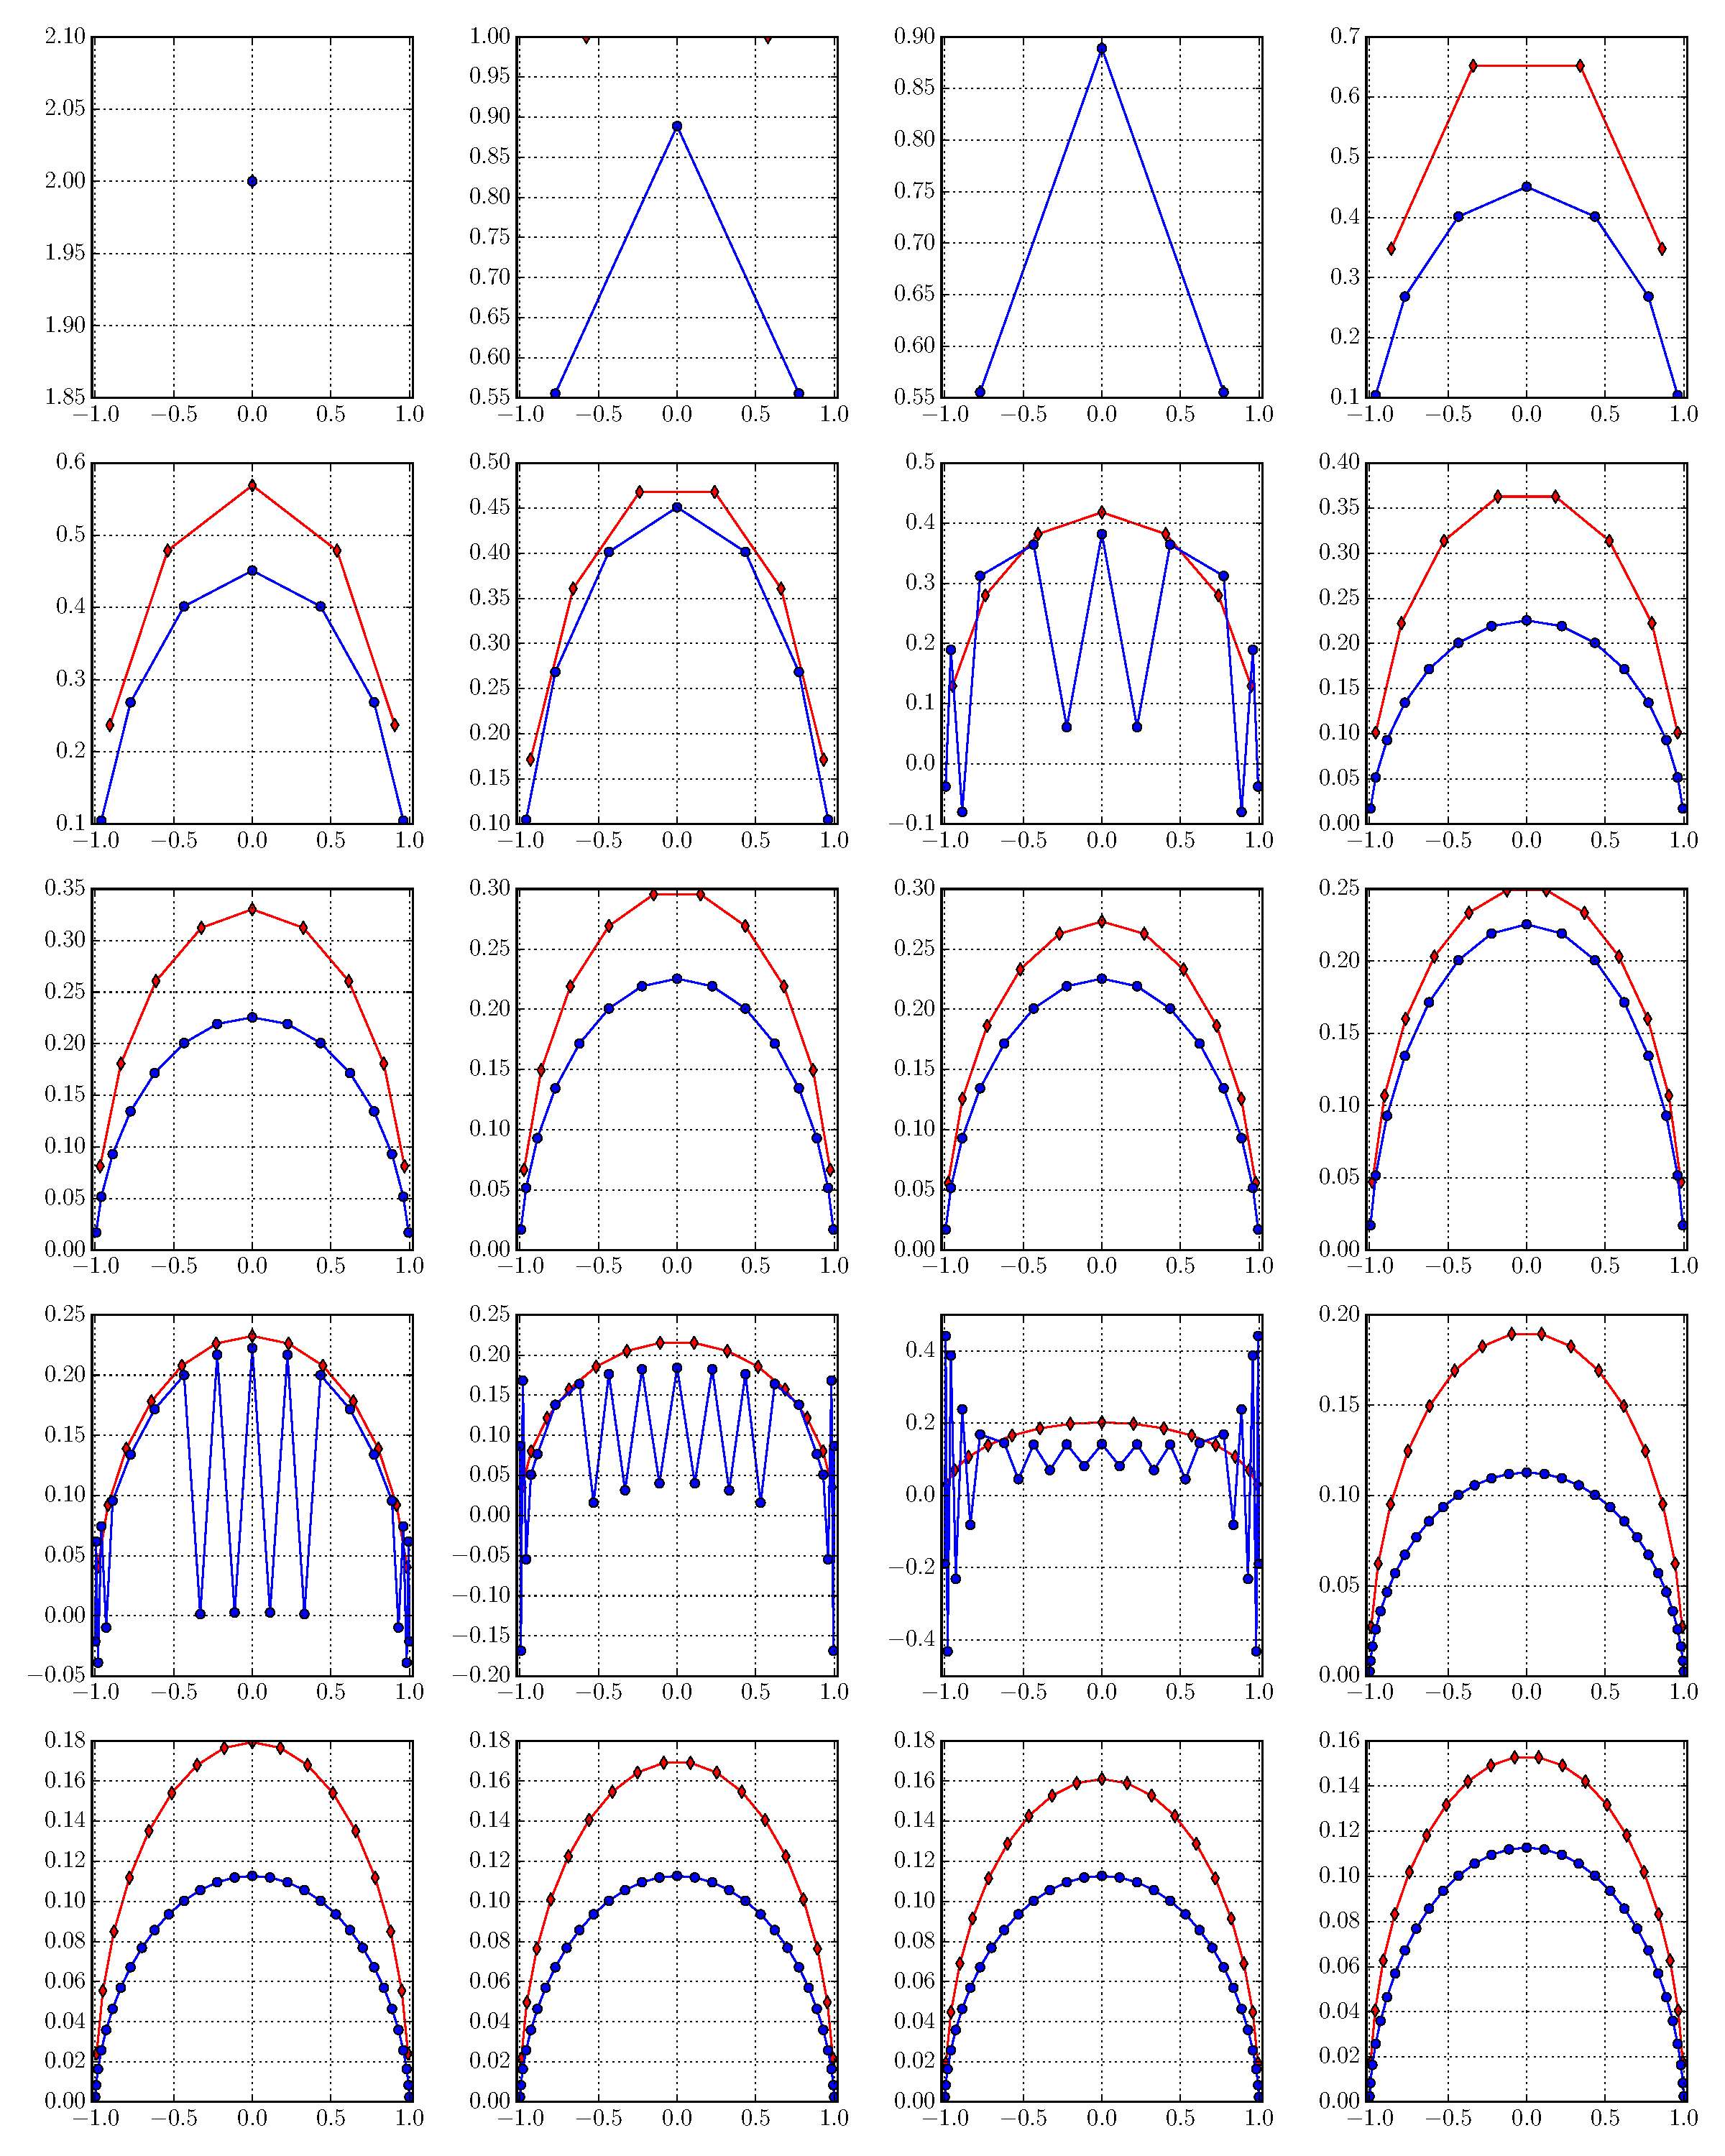
\includegraphics[width=\linewidth]{./img/gk_legendre_nodes_1d.pdf}
  \caption{Gauss-Legendre (red) and Genz-Keister (blue) nodes versus
  corresponding weights. The 1- and 3-point rules are identical.
  Note that a few rules have oscillations in the weights, some of them
  are almost zero, others become increasingly negative. This affects the
  stability of the corresponding rules.}
  \label{fig:gk_legendre_nodes_1d}
\end{figure}

\begin{figure}[h]
  \centering
  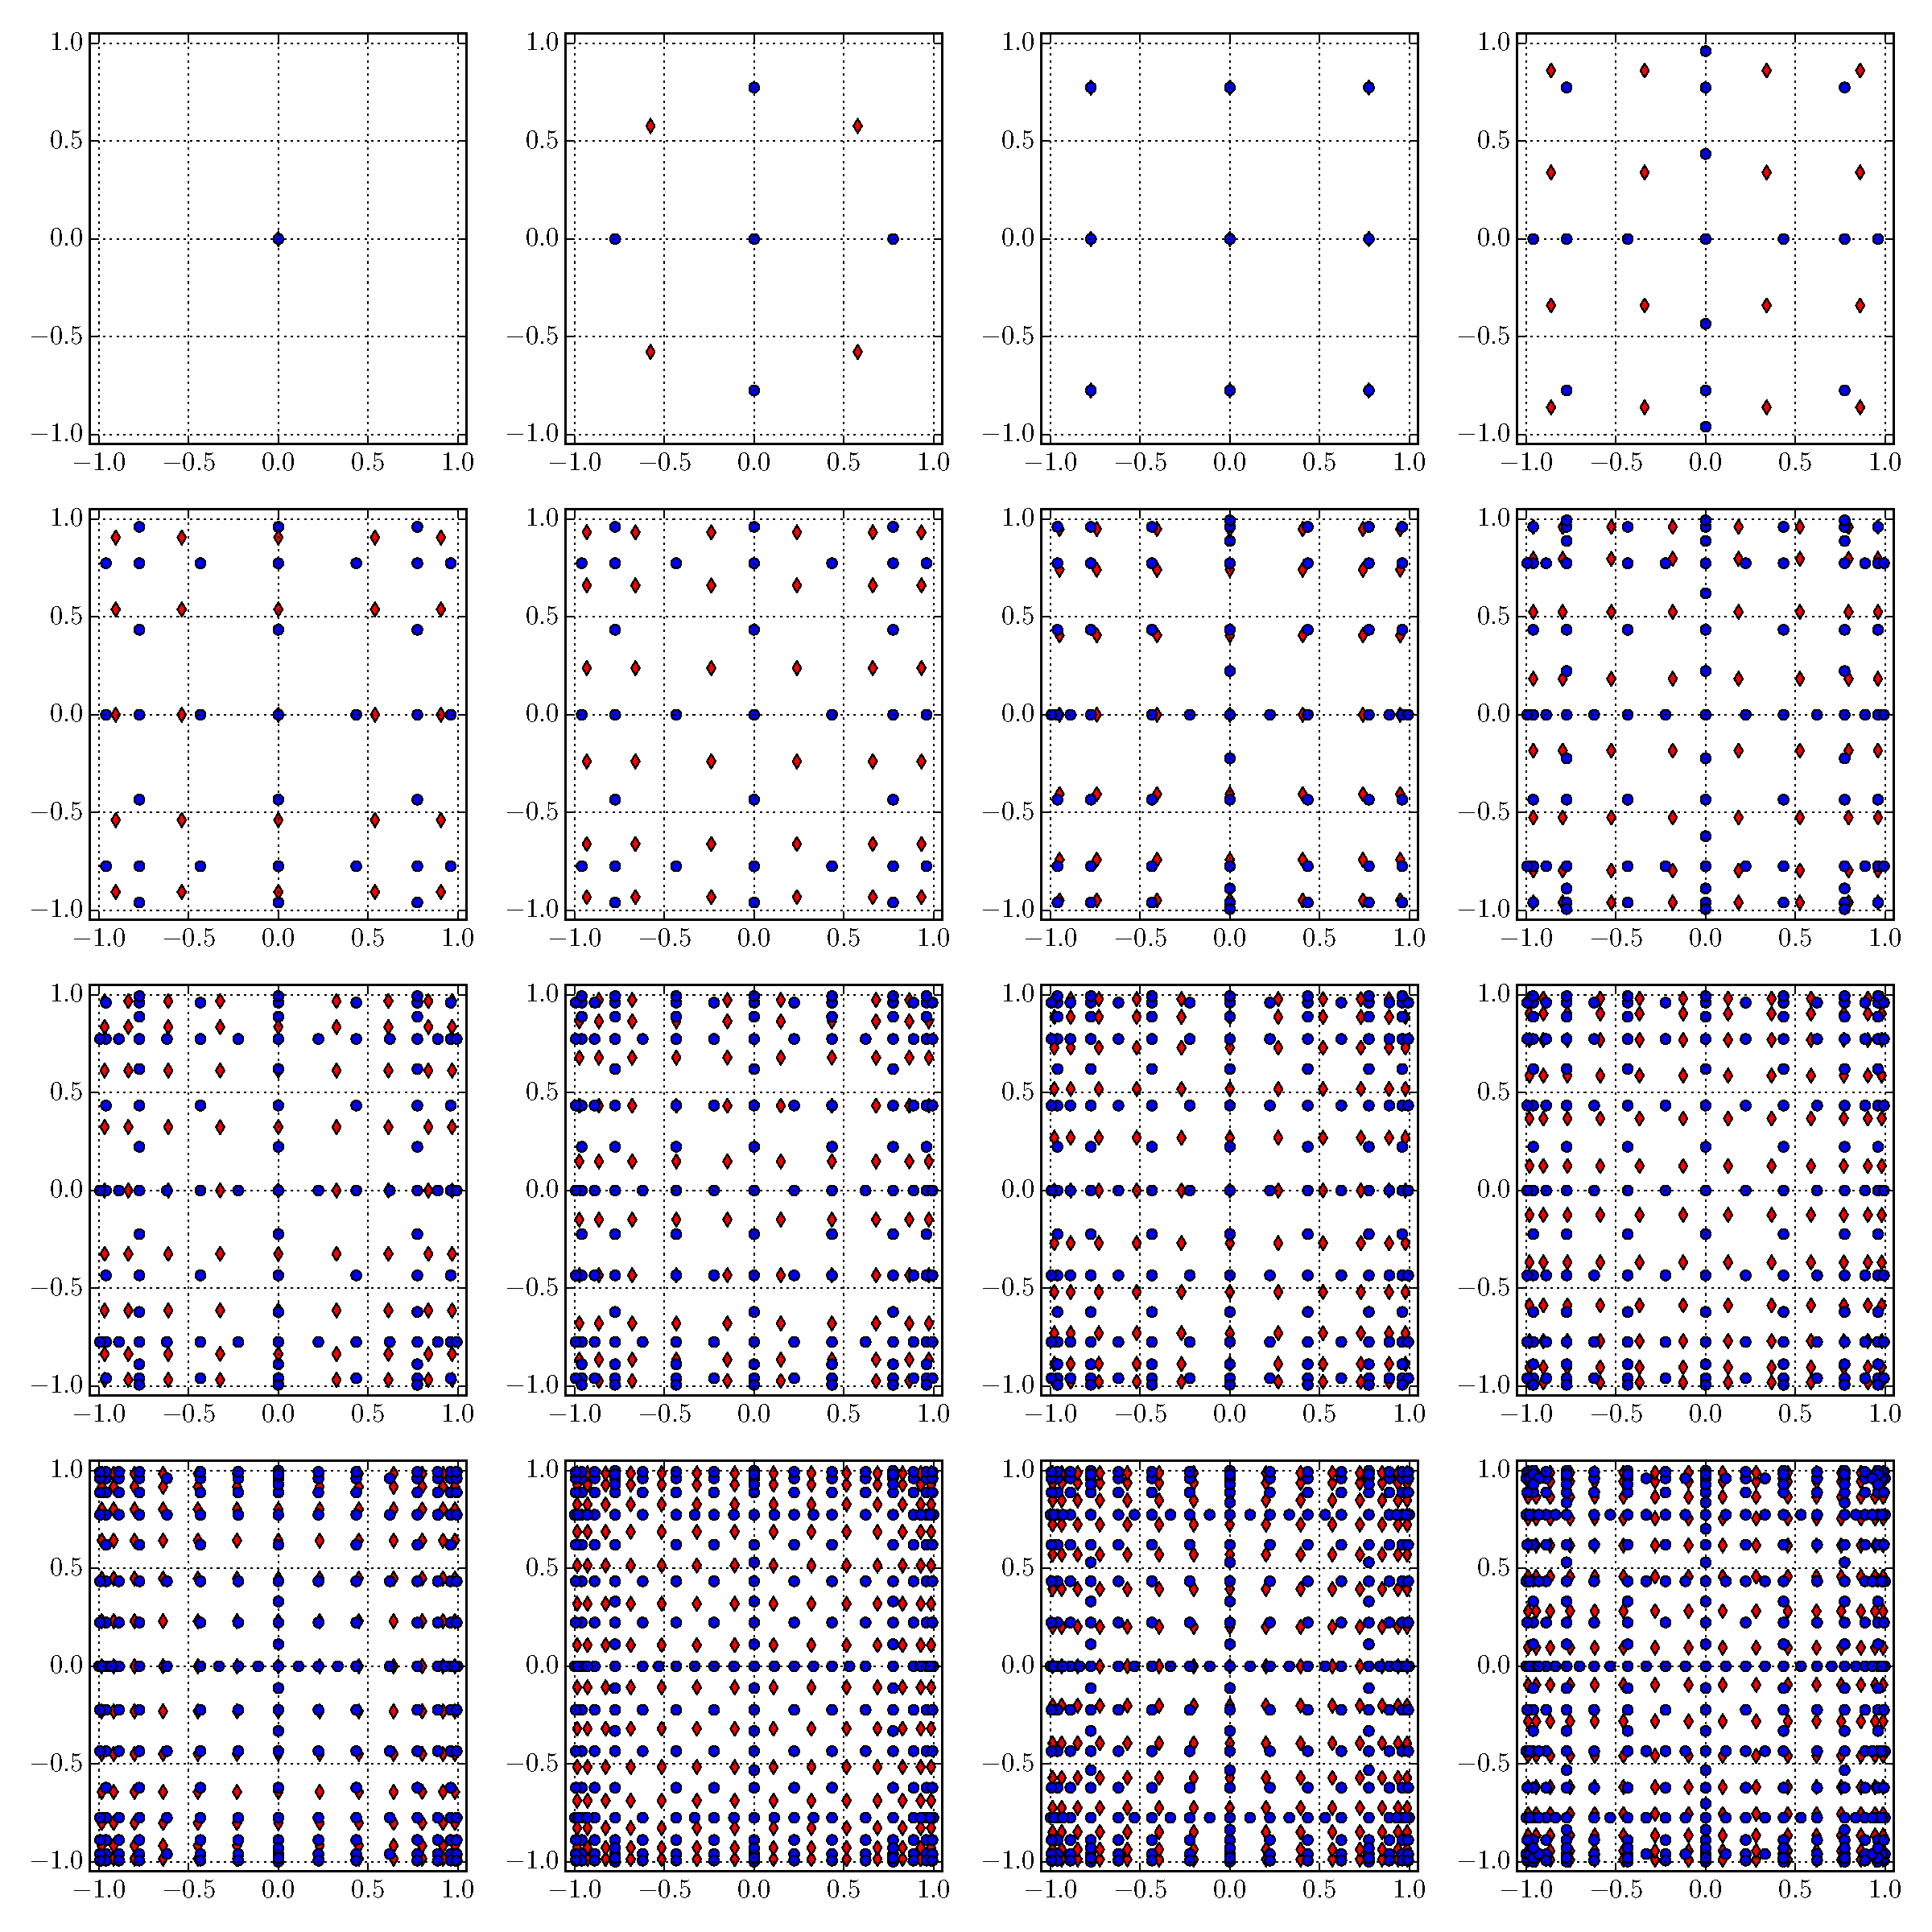
\includegraphics[width=\linewidth]{./img/gk_legendre_nodes_2d.pdf}
  \caption{Gauss-Legendre (red) and Genz-Keister (blue) nodes for
  two-dimensional rules. The Gauss-Legendre points form a full tensor
  product.}
  \label{fig:gk_legendre_nodes_2d}
\end{figure}

\begin{figure}
  \centering
  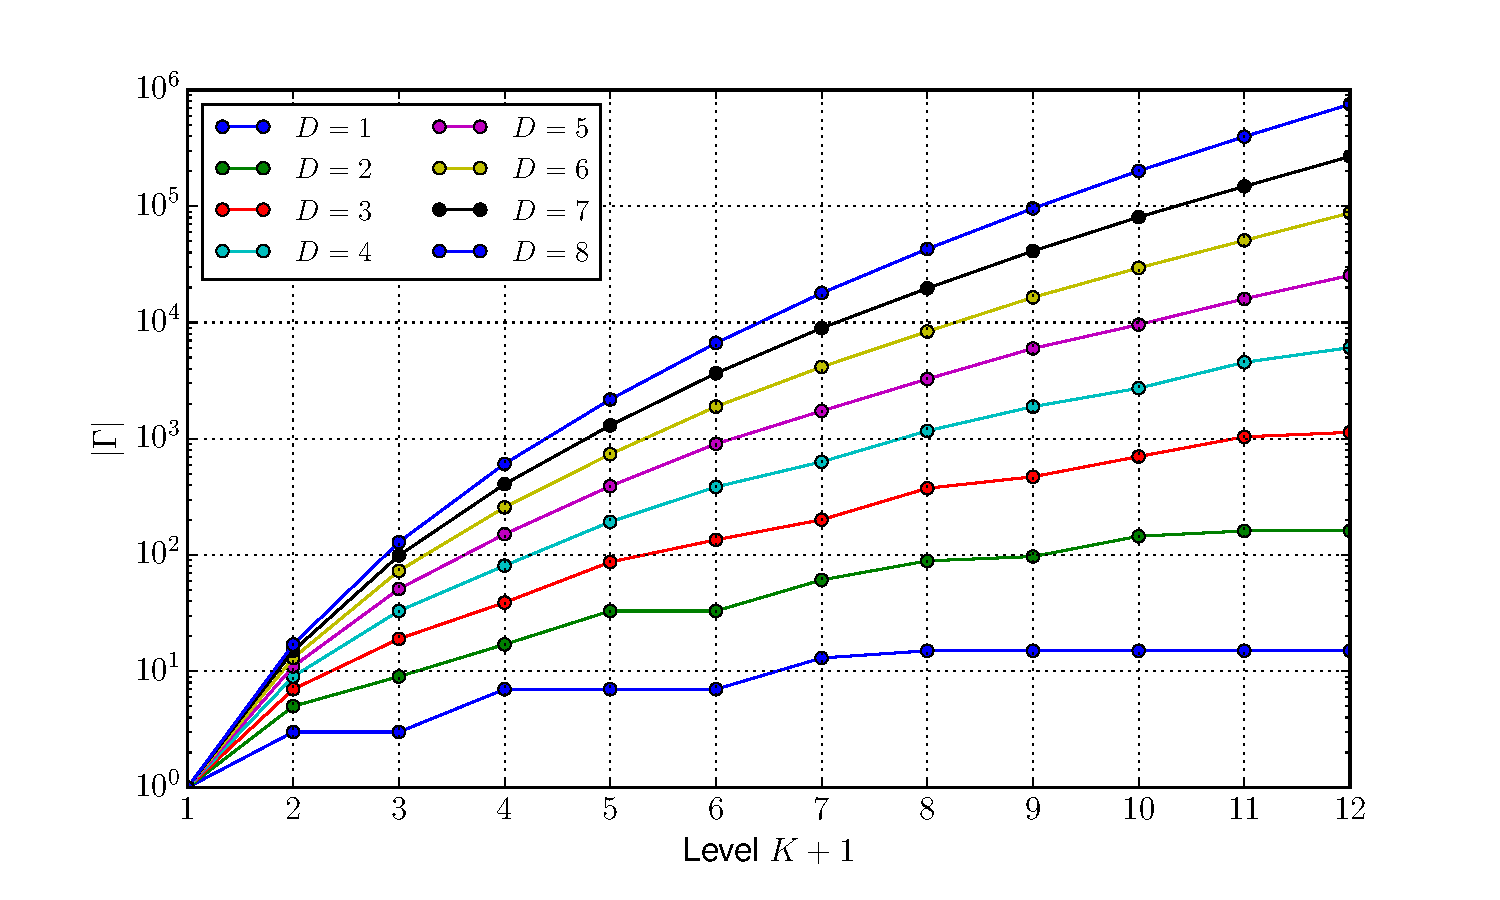
\includegraphics[width=\linewidth]{./img/number_nodes_levdim_legendre.pdf}
  \caption{Number $|\Gamma|$ of Genz-Keister quadrature nodes for various levels $K$ and dimensions $D$.}
  \label{fig:number_nodes_levdim_legendre}
\end{figure}

\begin{figure}[h]
  \centering
  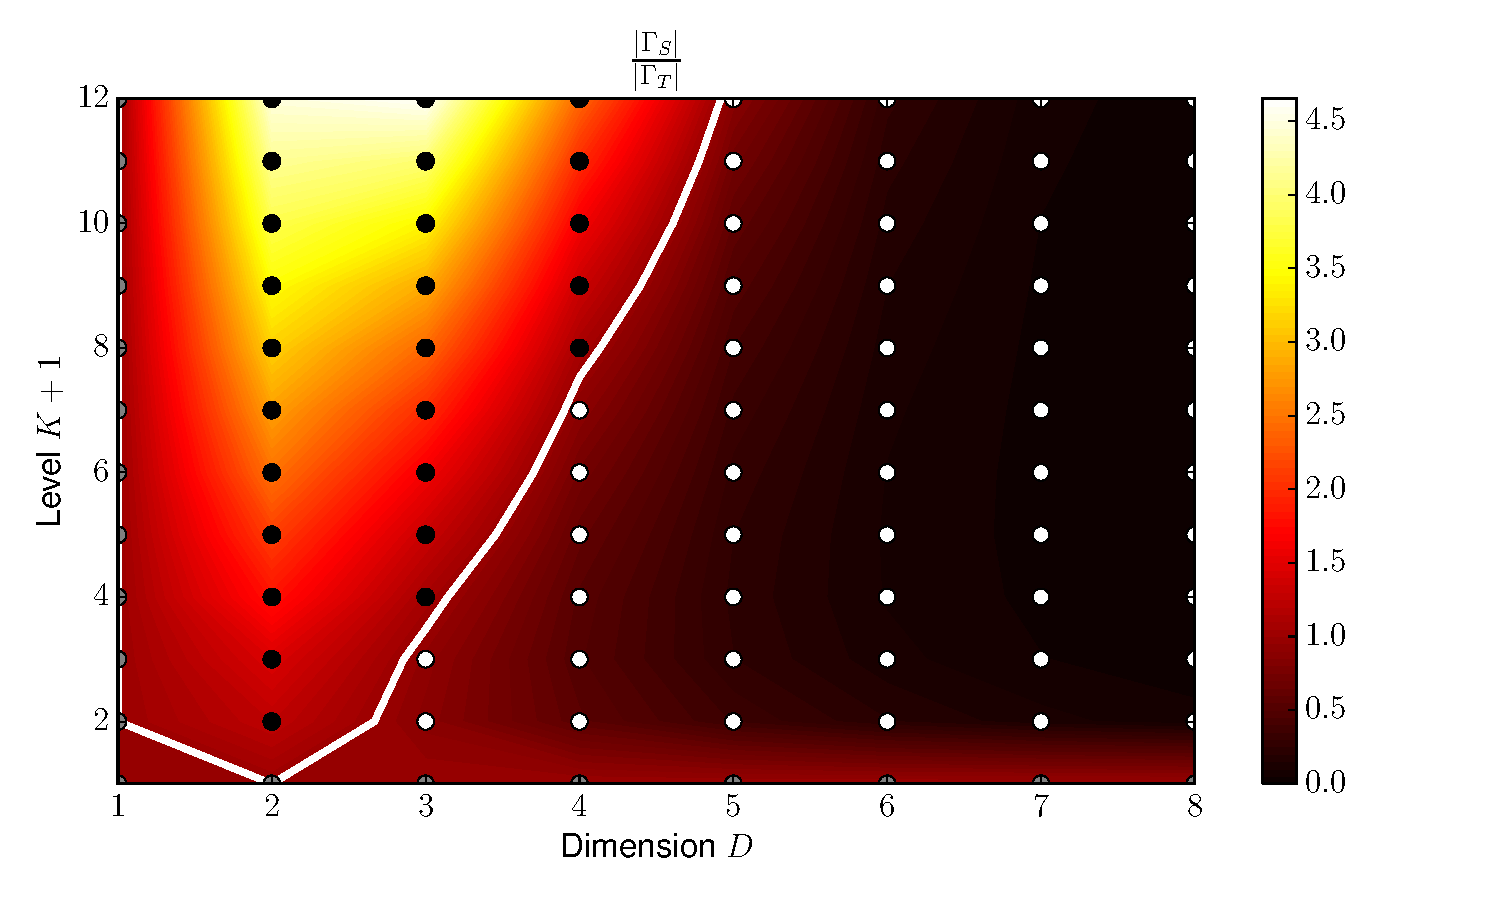
\includegraphics[width=0.8\linewidth]{./img/smol_legendre_ratio.pdf}
  \caption{Ratio of the number of Gauss-Legendre quadrature points obtained
  via tensor product and classical Smolyak construction. White dots are $D,K$
  combinations where Genz-Keister is advantageous, while for black dots
  Genz-Keister is worse and for gray dots the ratio equals 1.}
  \label{fig:smol_legendre_ratio}
\end{figure}

\begin{figure}[h]
  \centering
  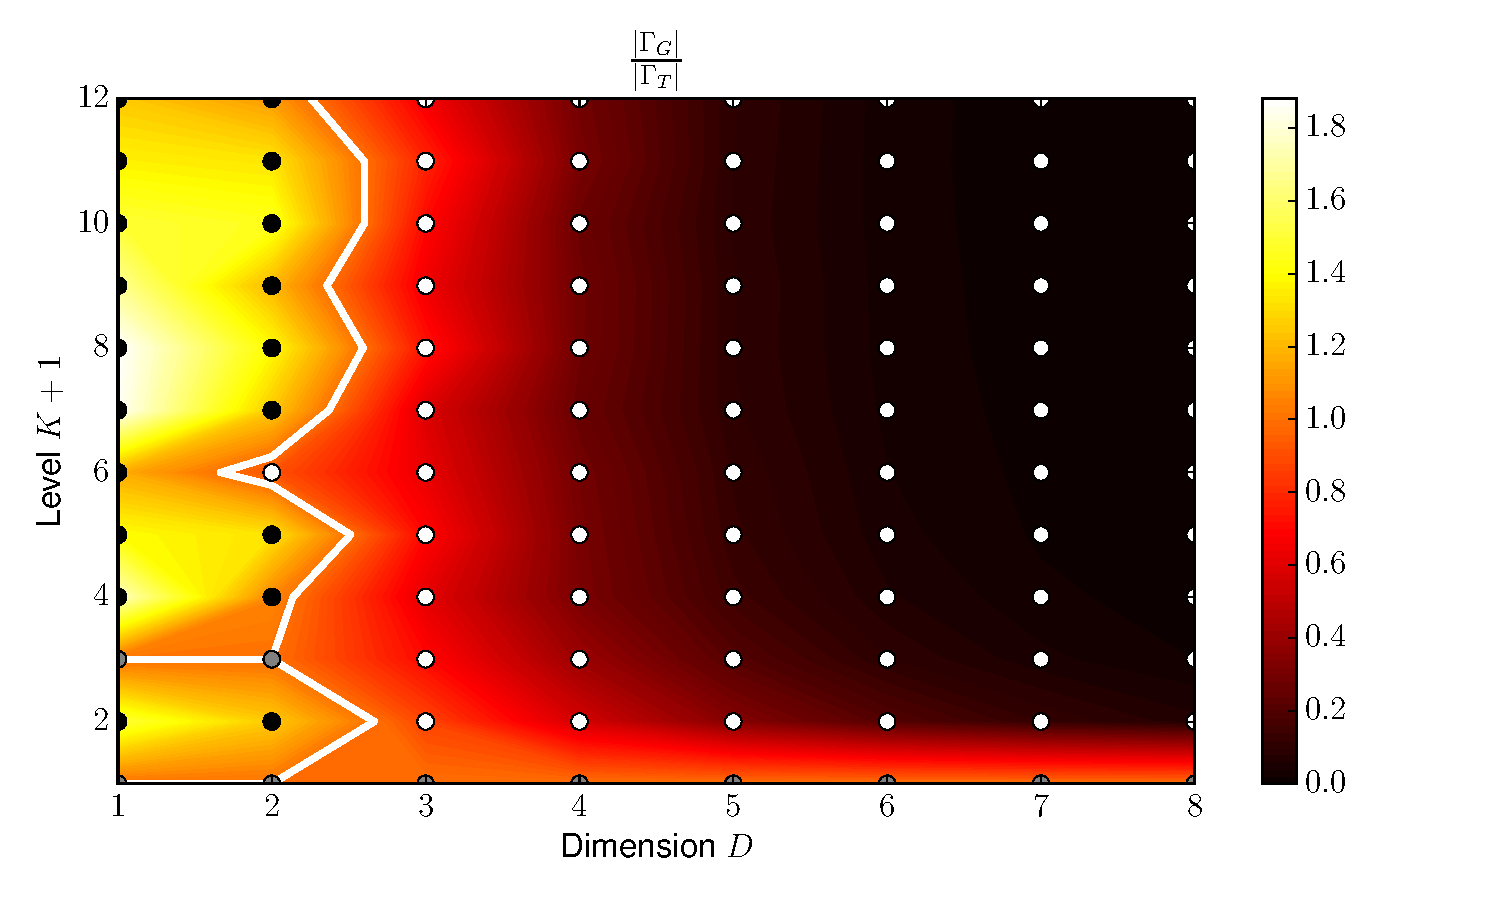
\includegraphics[width=0.8\linewidth]{./img/gk_legendre_ratio.pdf}
  \caption{Ratio of the number of Genz-Keister and Gauss-Legendre tensor product
  points for dimensions $D$ up to 8 and Level $K \leq 12$. White dots are $D,K$
  combinations where Genz-Keister is advantageous, while for black dots
  Genz-Keister is worse and for gray dots the ratio equals 1.}
  \label{fig:gk_legendre_ratio}
\end{figure}

\begin{figure}[h]
  \centering
  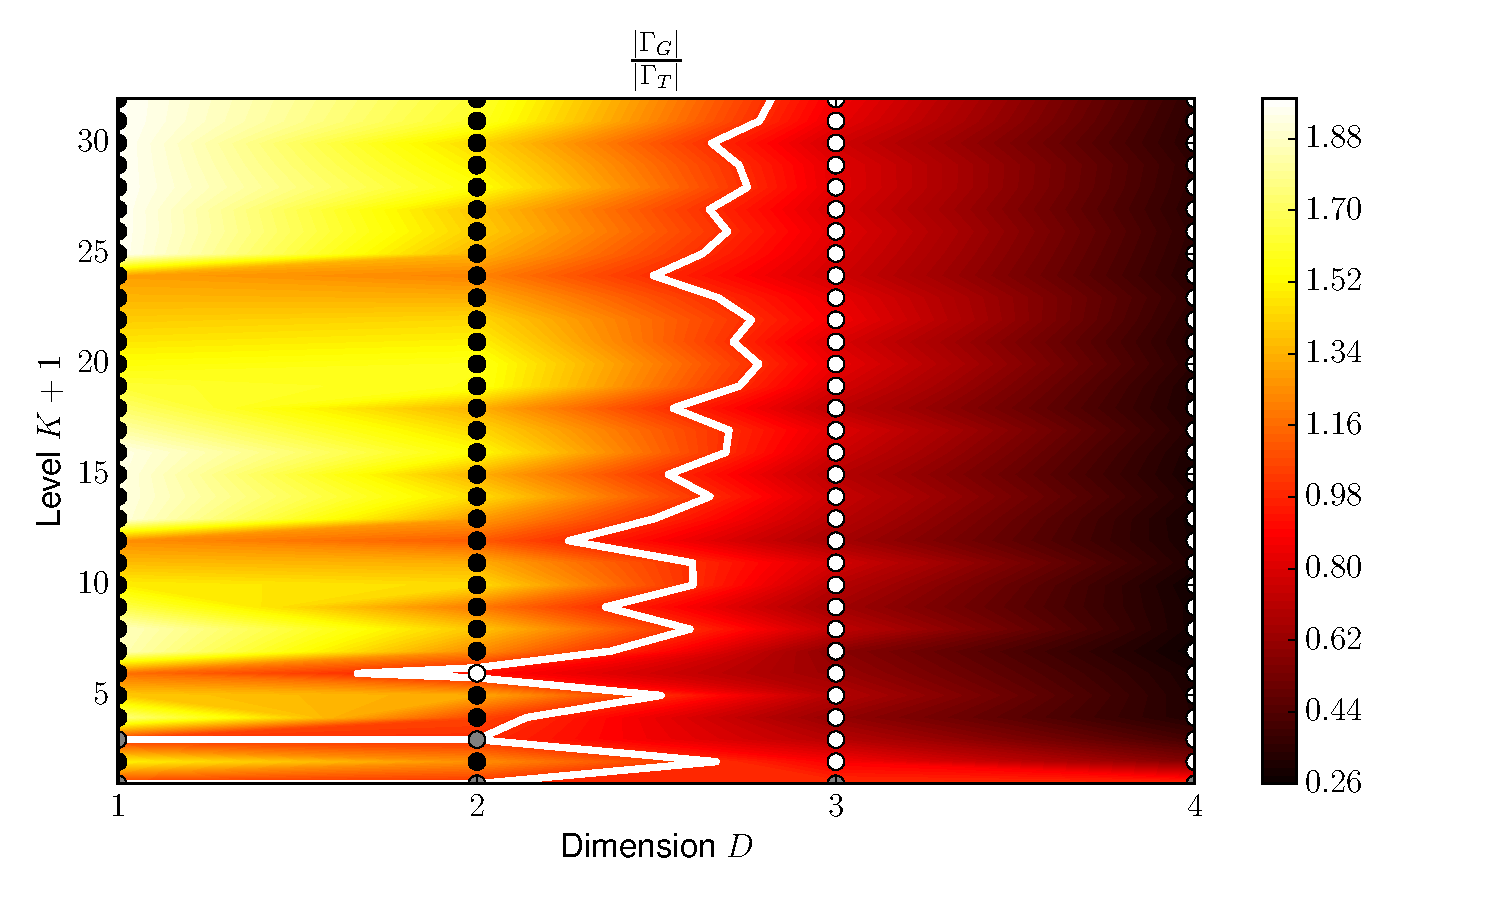
\includegraphics[width=0.8\linewidth]{./img/gk_legendre_ratio_large.pdf}
  \caption{Ratio of the number of Genz-Keister and Gauss-Legendre tensor product
  points for dimensions 1 to 4 and Level $K \leq 32$. White dots are $D,K$
  combinations where Genz-Keister is advantageous, while for black dots
  Genz-Keister is worse and for gray dots the ratio equals 1. Notice the tendency
  of the white boundary to go to the right and eventually reach dimensions $D \geq 3$.}
  \label{fig:gk_legendre_ratio_large}
\end{figure}

\begin{figure}[h]
  \centering
  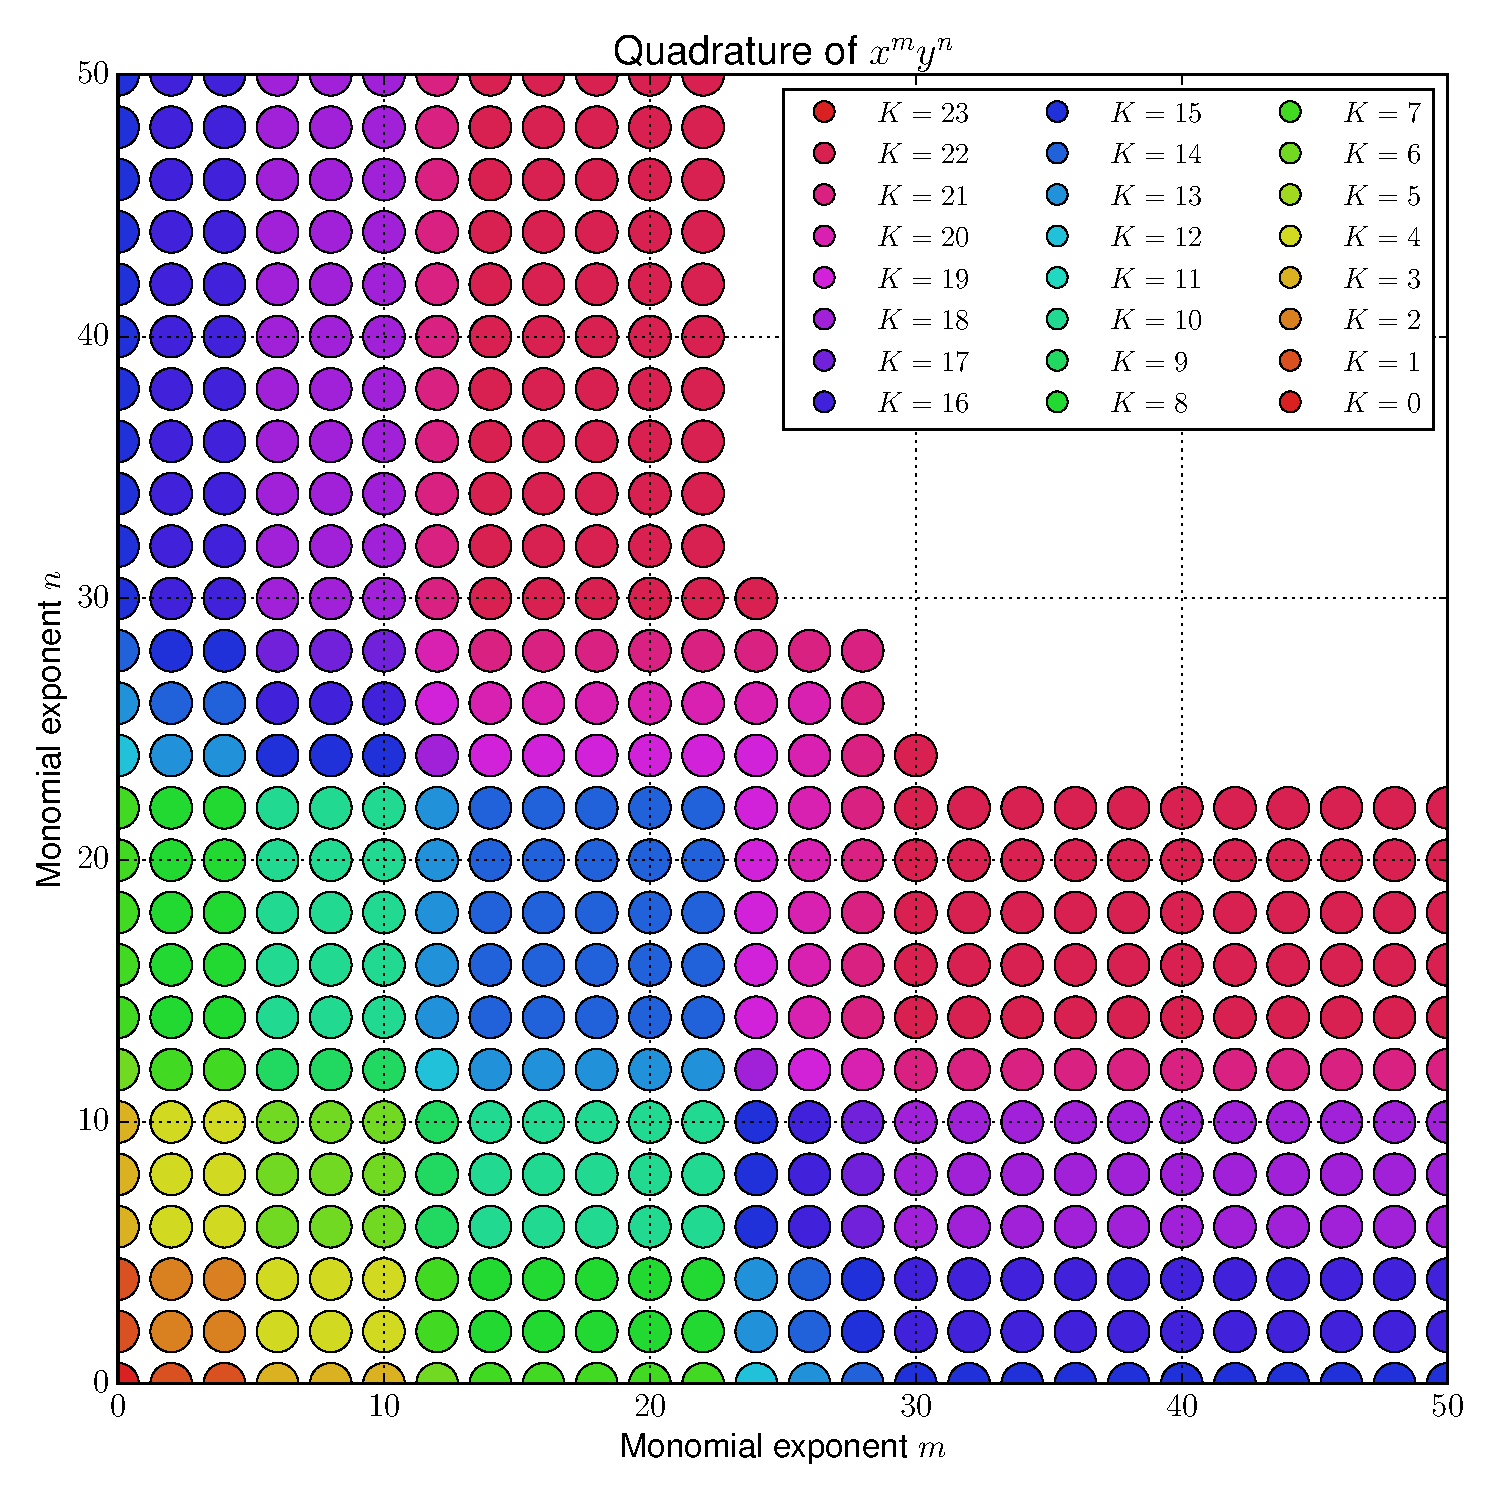
\includegraphics[width=\linewidth]{./img/monomial_errors_legendre_2D.pdf}
  \caption{Quadrature of the bivariate monomials $x^m y^n$ for $0 \leq n, m \leq 50$.
  Each pair $(m,n)$ is color-coded by the lowest level $K$ rule that correctly
  integrates the monomial with a relative error not larger than $10^{-13}$.}
  \label{fig:monomial_errors_legendre_2D}
\end{figure}

For testing the quadrature rules in $D$ dimensions, the following integral
over multi-variate monomials with $\vec{n} \in \mathbb{N}_0^D$ is used:
\begin{equation} \label{eq:legendre_exact_solution}
  \idotsint \limits_{\vec{x} \in [-1,1]^D} \prod_{d=1}^D x_d^{n_d} \di{\vec{x}}
  =
  \prod_{d=1}^D \frac{1 + (-1)^{n_d}}{1 + n_d}
\end{equation}
where we know the exact solution in closed form.

\begin{subfigures}
  \label{fig:monomial_errors_legendre_multivariate}
  \begin{figure}\centering
    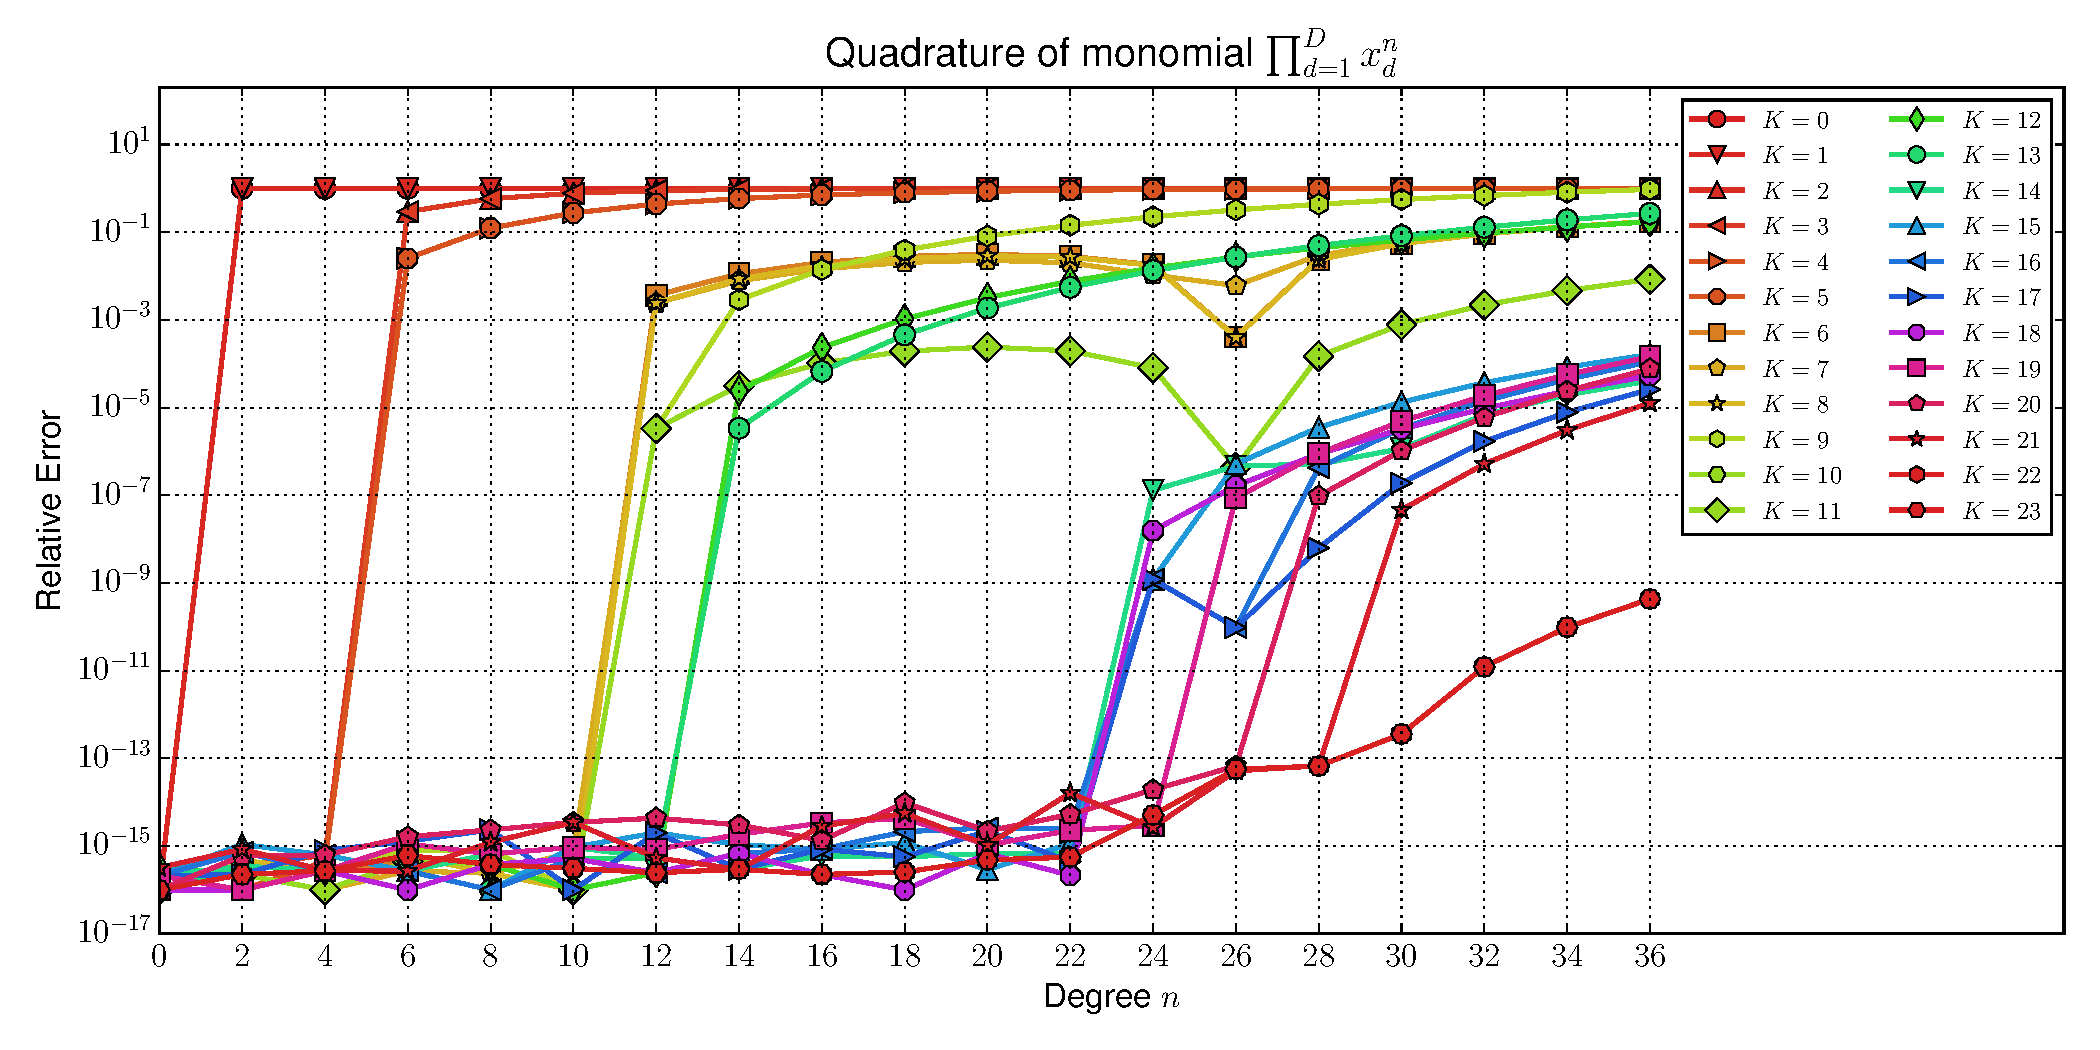
\includegraphics[width=\linewidth]{./img/monomial_errors_legendre_multivariate_dimension_2.pdf}
    \caption{Relative errors for the integral \eqref{eq:legendre_exact_solution}
    in $D=2$ dimensions. All variables $x_d$ share the same exponent $n$.}
    \label{fig:monomial_errors_legendre_multivariate_dimension_2}
  \end{figure}
  \begin{figure}\centering
    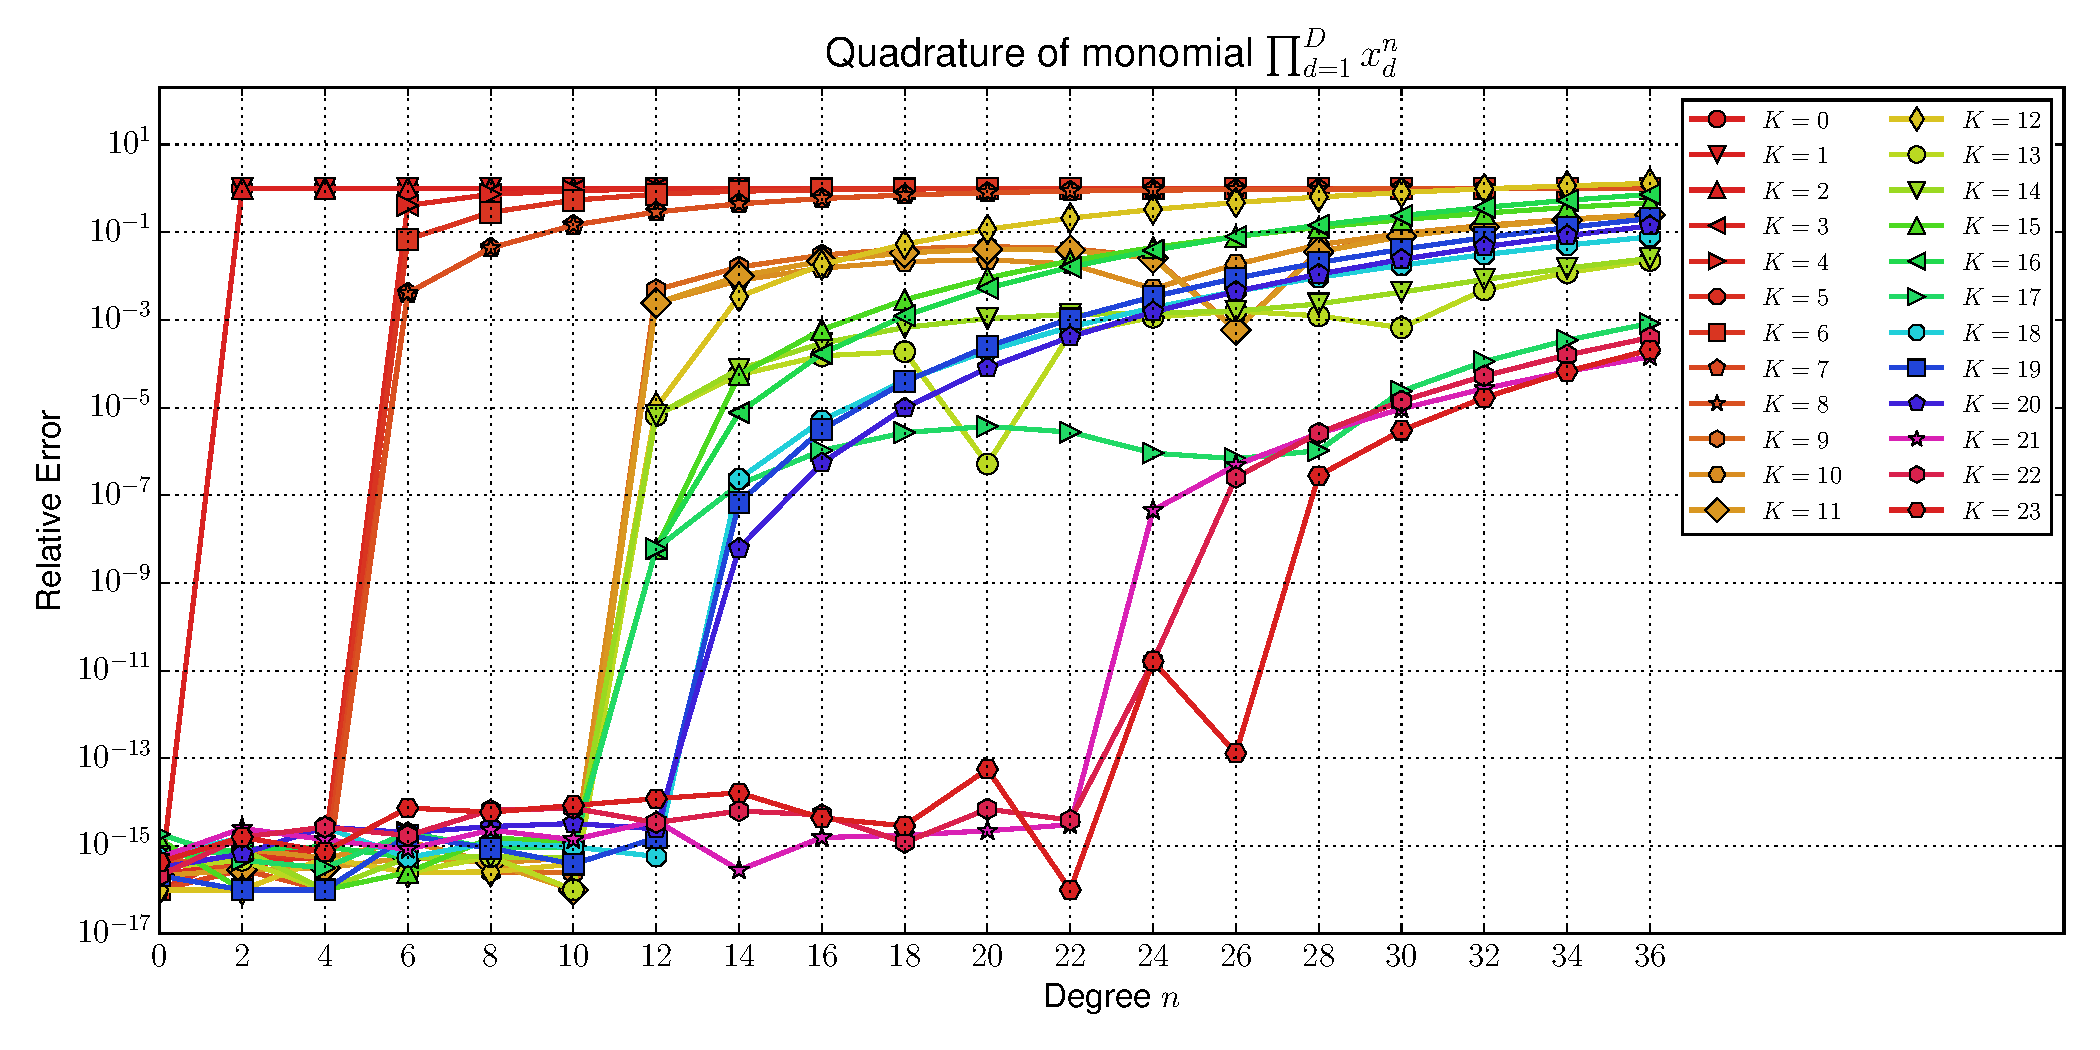
\includegraphics[width=\linewidth]{./img/monomial_errors_legendre_multivariate_dimension_3.pdf}
    \caption{Relative errors for the integral \eqref{eq:legendre_exact_solution}
    in $D=3$ dimensions. All variables $x_d$ share the same exponent $n$.}
    \label{fig:monomial_errors_legendre_multivariate_dimension_3}
  \end{figure}
  \begin{figure}\centering
    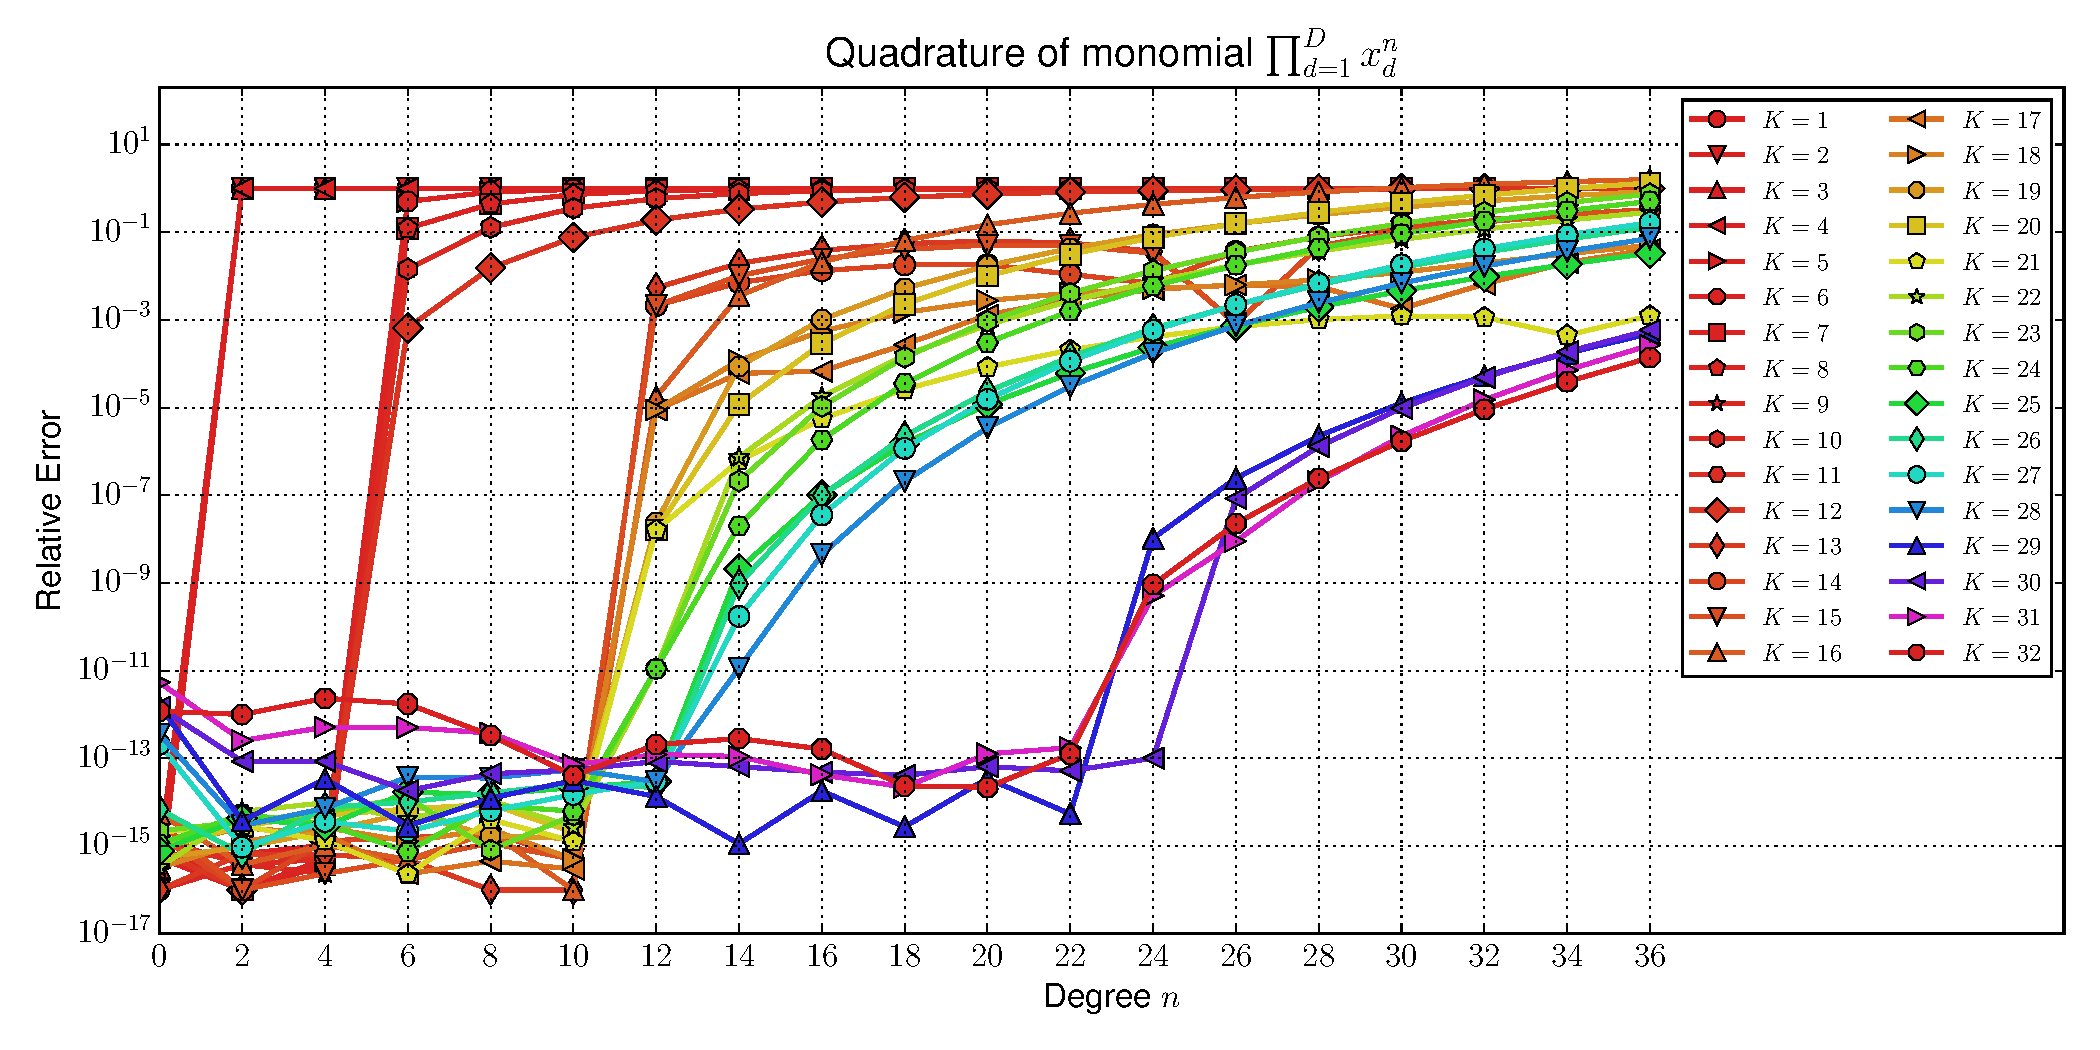
\includegraphics[width=\linewidth]{./img/monomial_errors_legendre_multivariate_dimension_4.pdf}
    \caption{Relative errors for the integral \eqref{eq:legendre_exact_solution}
    in $D=4$ dimensions. All variables $x_d$ share the same exponent $n$.}
    \label{fig:monomial_errors_legendre_multivariate_dimension_4}
  \end{figure}
  \begin{figure}\centering
    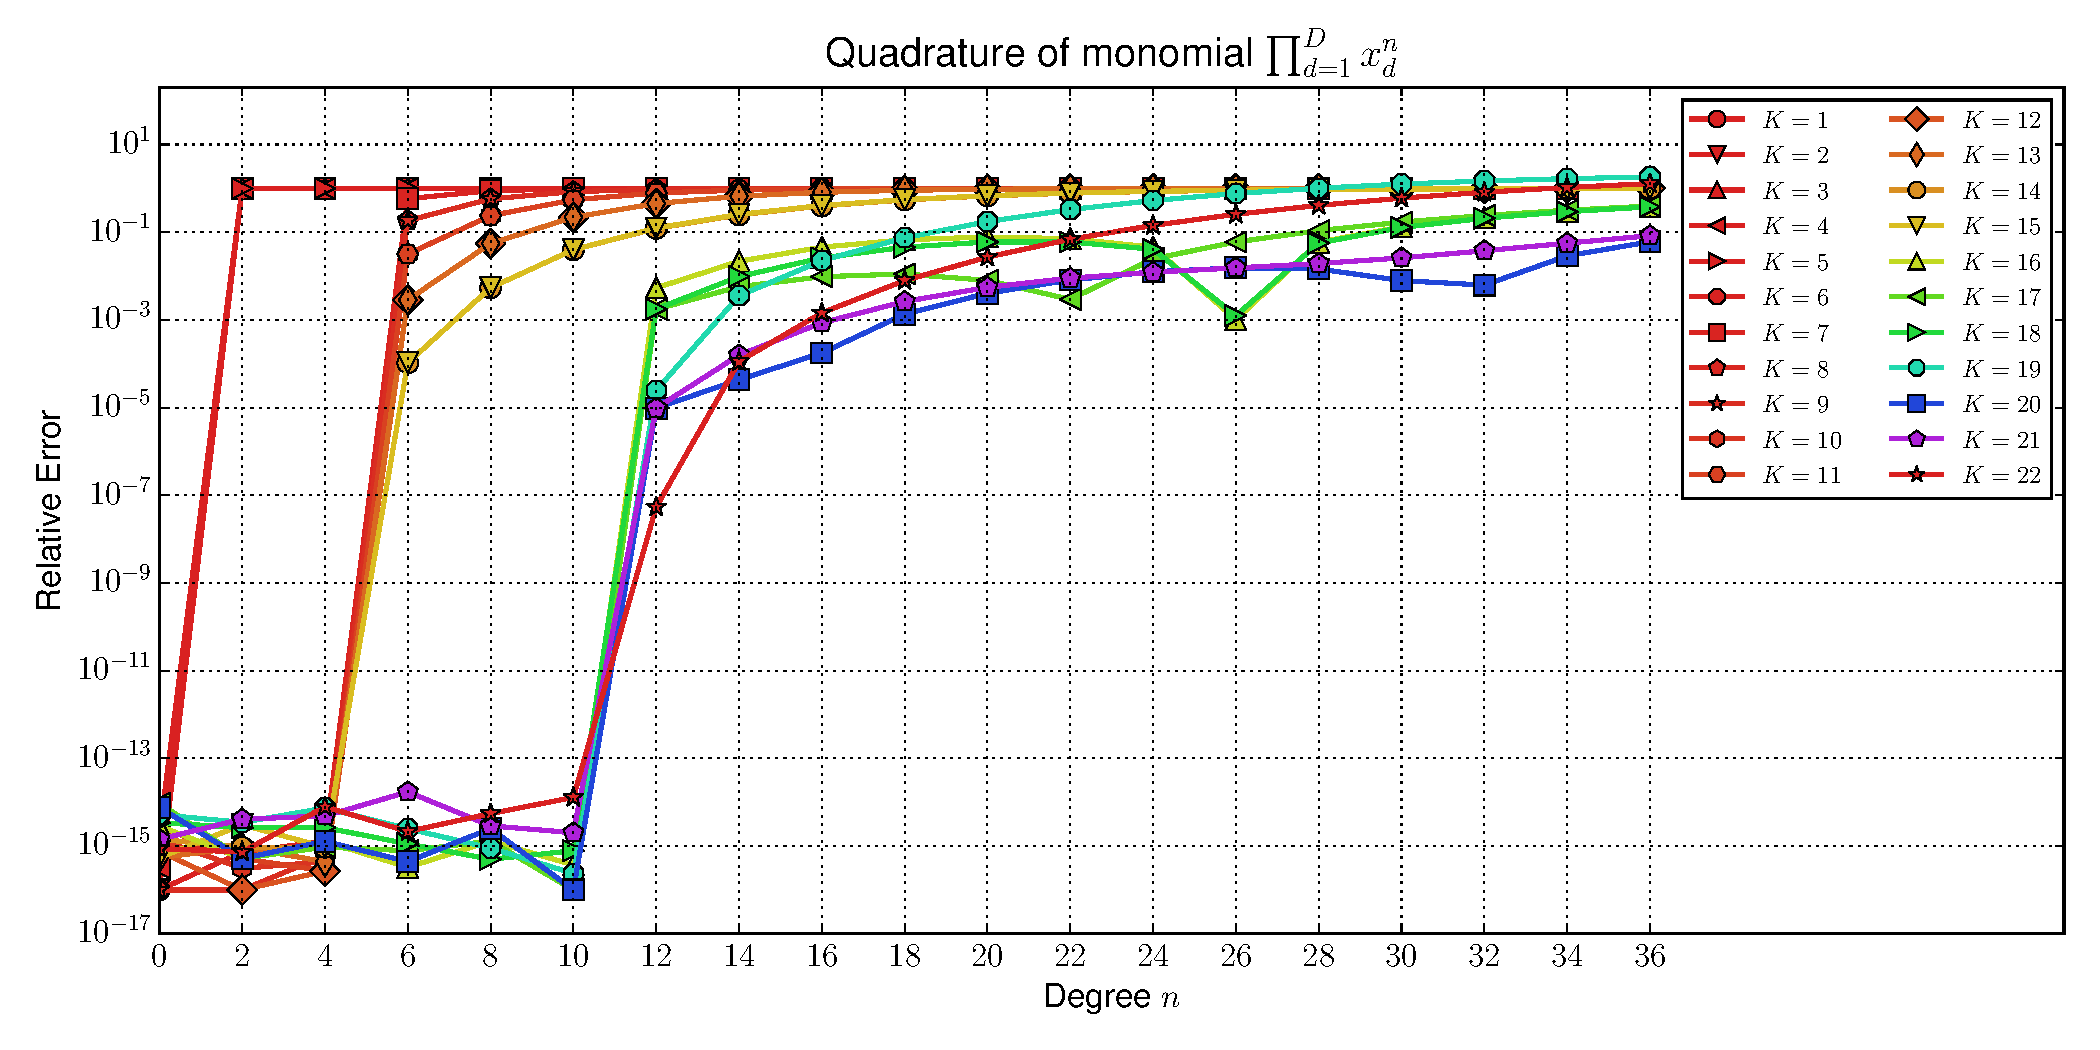
\includegraphics[width=\linewidth]{./img/monomial_errors_legendre_multivariate_dimension_5.pdf}
    \caption{Relative errors for the integral \eqref{eq:legendre_exact_solution}
    in $D=5$ dimensions. All variables $x_d$ share the same exponent $n$.}
    \label{fig:monomial_errors_legendre_multivariate_dimension_5}
  \end{figure}
  \begin{figure}\centering
    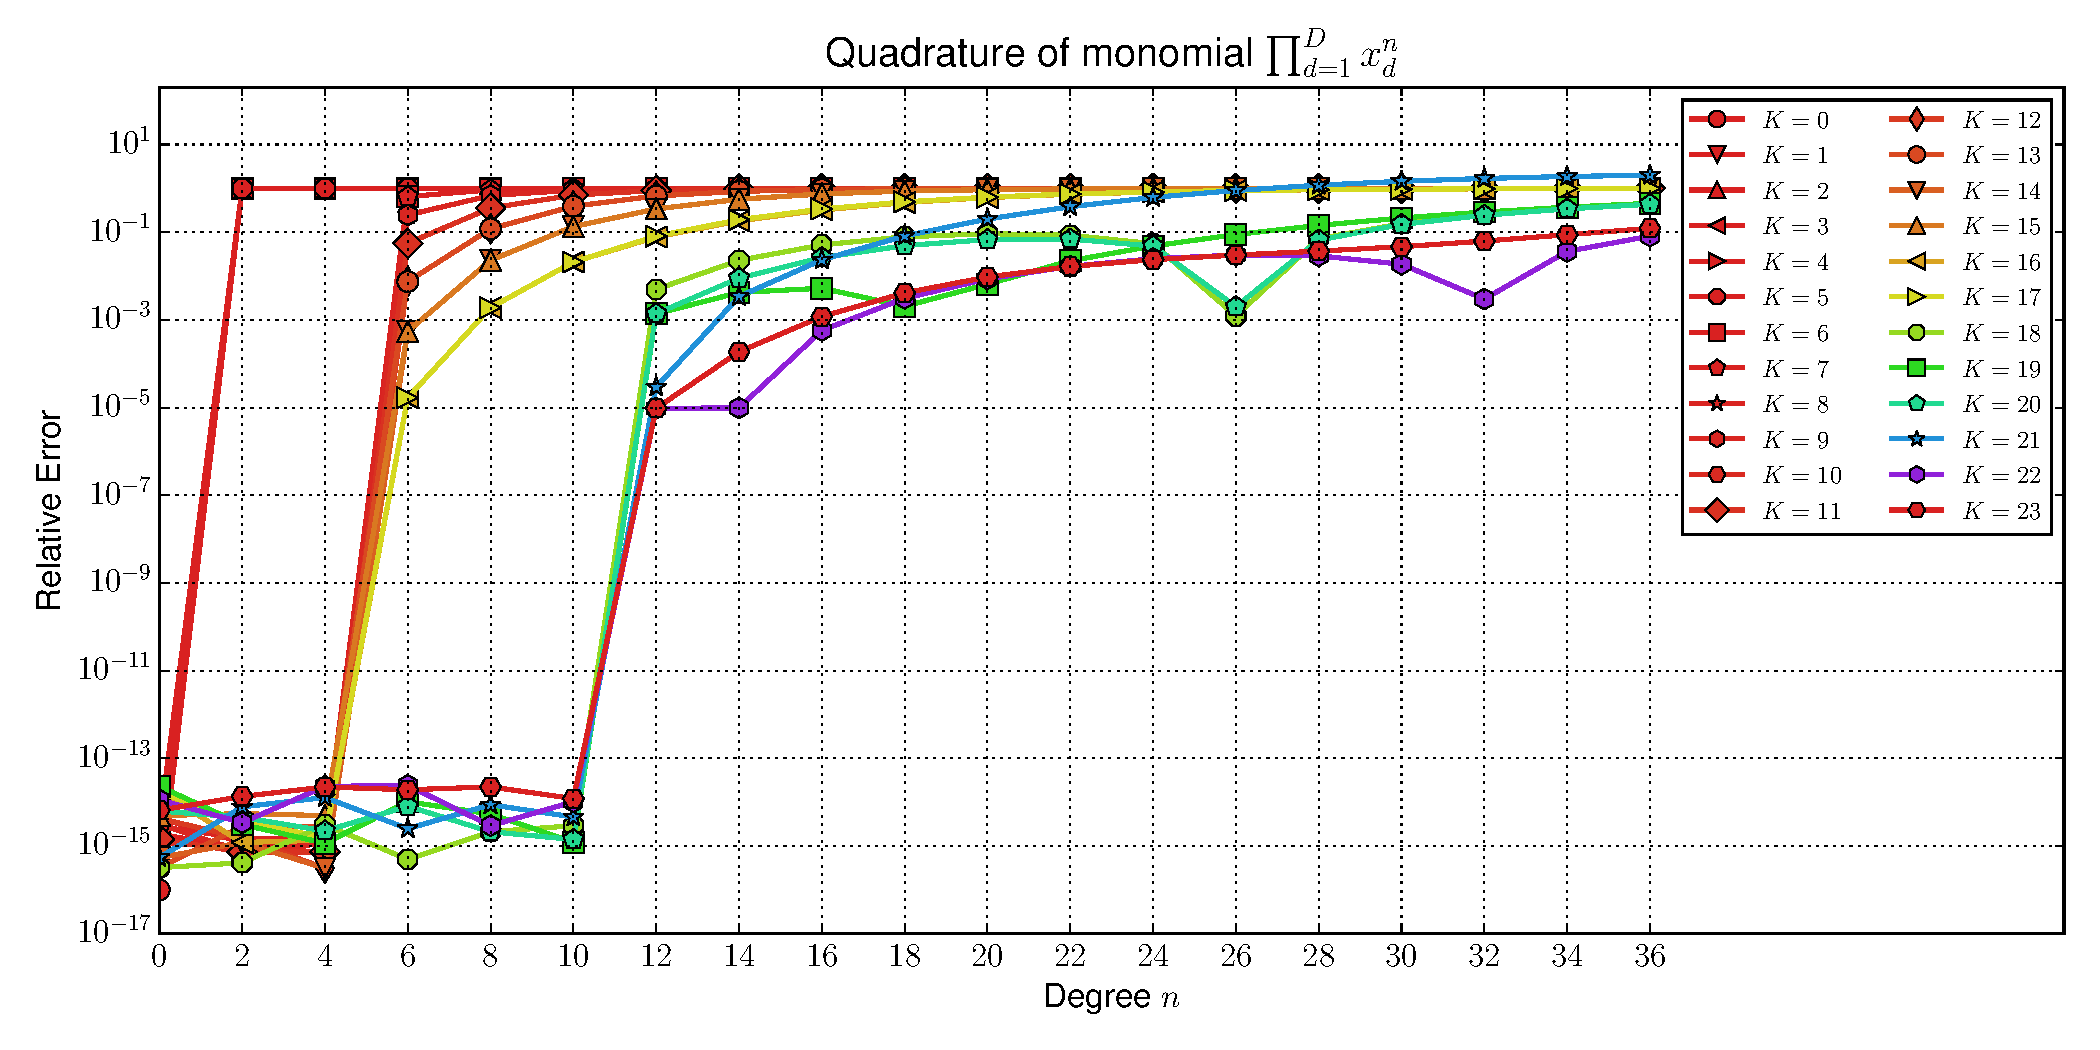
\includegraphics[width=\linewidth]{./img/monomial_errors_legendre_multivariate_dimension_6.pdf}
    \caption{Relative errors for the integral \eqref{eq:legendre_exact_solution}
    in $D=6$ dimensions. All variables $x_d$ share the same exponent $n$.}
    \label{fig:monomial_errors_legendre_multivariate_dimension_6}
  \end{figure}
\end{subfigures}

\FloatBarrier
\subsection{Chebyshev Quadrature of the first kind}

As in the case of Legendre polynomials, both Chebyshev polynomials $T_n$
and $U_n$ possess many different Kronrod extensions. For the first kind $T_n$
we choose $\mathcal{K} = (1, 2, 4, 6, 12, 24)$ with the $\vec{z}$ sequence:
\begin{equation*}
  \vec{z} = (0, 0, 1, 0, 2, 1, 0, 5, 4, 3, 2, 1, 0, 11, 10, 9, 8, 7, 6, 5, 4, 3, 2, 1, 0, 1) \,.
\end{equation*}
Again we can in principle extend $\mathcal{K}$ by doubling the degree.
Using this extension we get the one-dimensional quadrature nodes and weights shown
in Figure \ref{fig:gk_chebyshevt_nodes_1d}.
Figure \ref{fig:gk_chebyshevt_nodes_2d} shows the sparse
node distribution in the plane for two-dimensional quadrature rules.
Notice that for $D < 3$, using the Genz-Keister construction results
in more quadrature points than the full tensor product Ansatz, however there
are some exceptions. This fact is examined in Figures \ref{fig:gk_chebyshevt_ratio}
and \ref{fig:gk_chebyshevt_ratio_large}.

\begin{figure}[h]
  \centering
  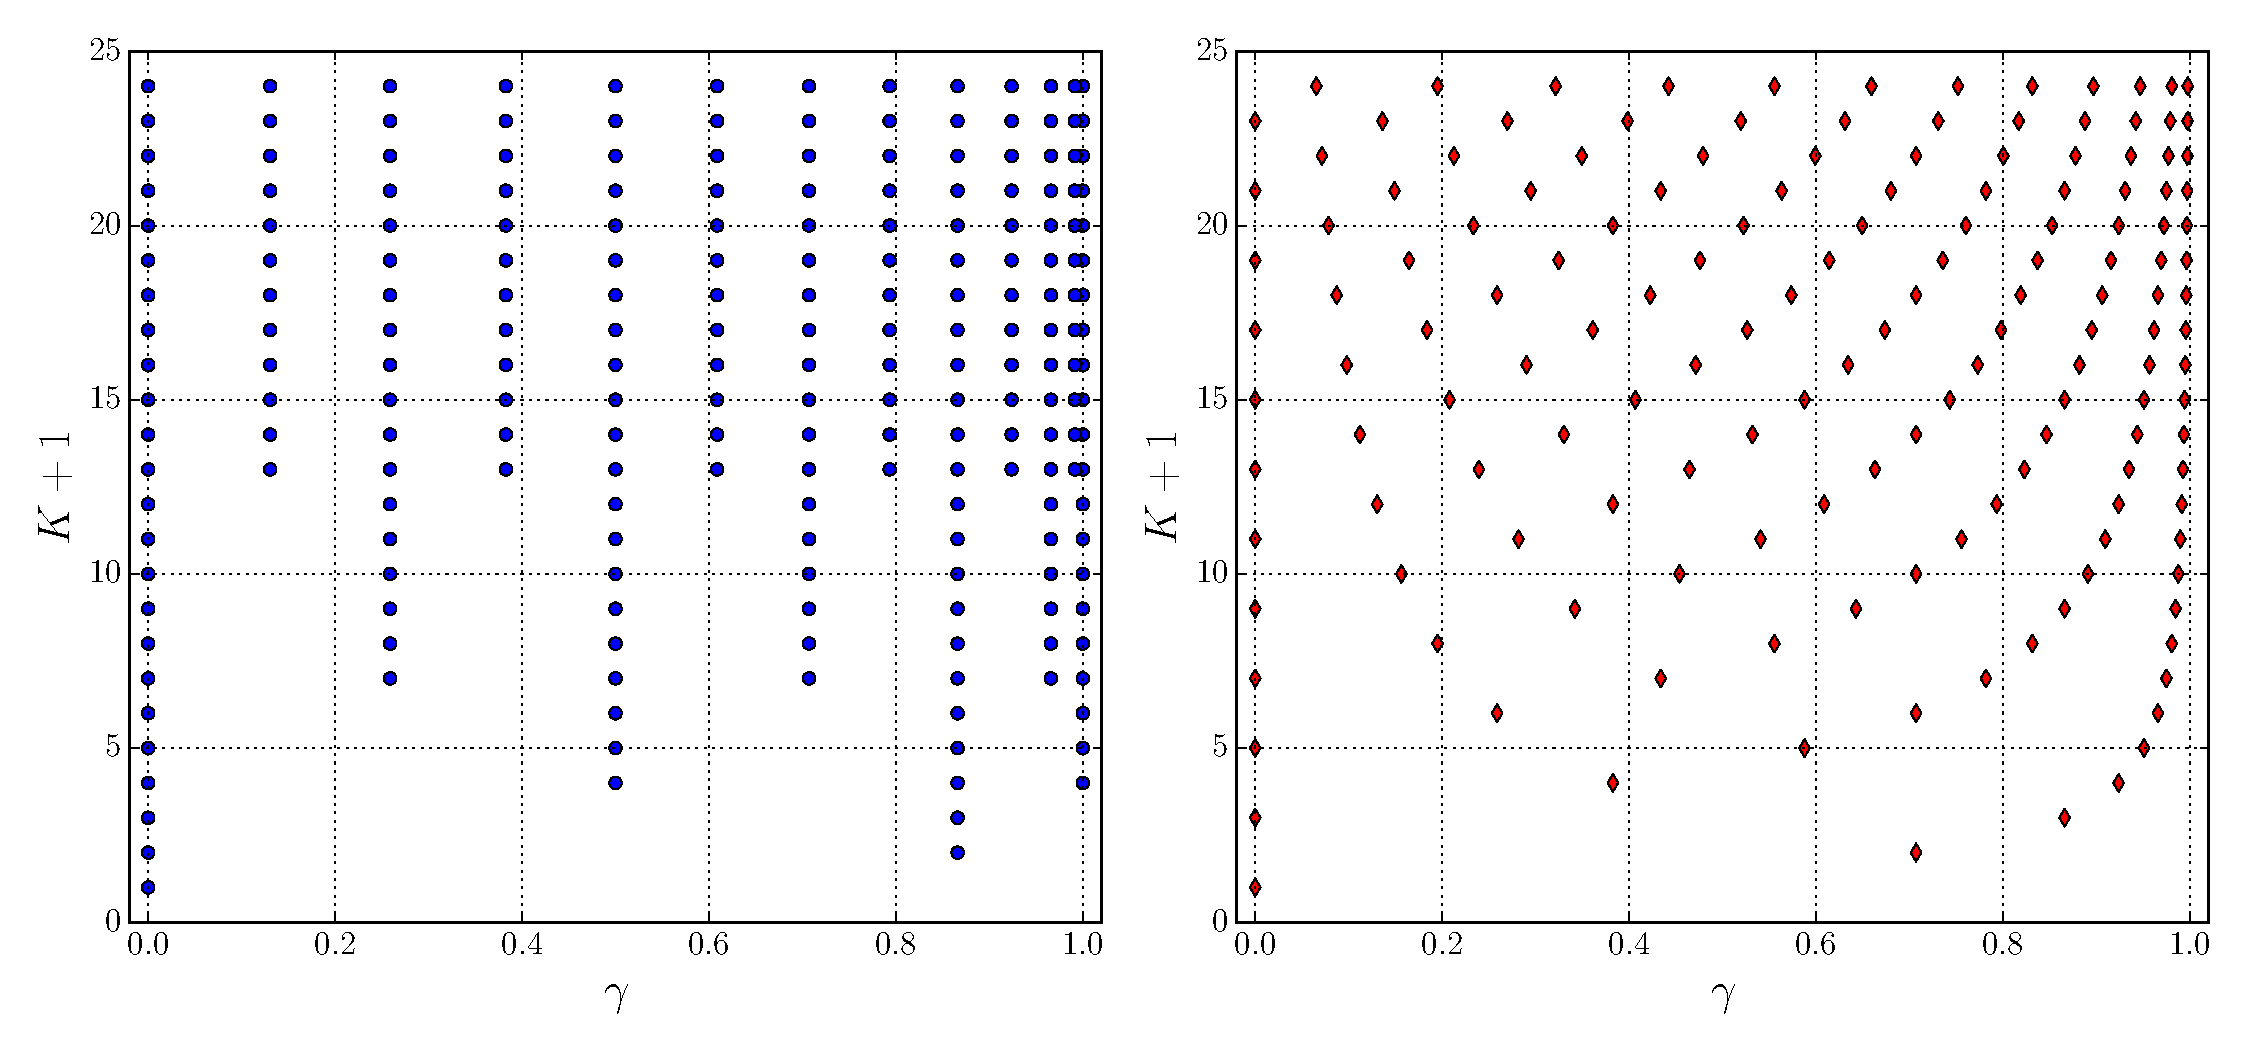
\includegraphics[width=\linewidth]{./img/gk_chebyshevt_nodes_cmp.pdf}
  \caption{Comparison of Gauss-Chebyshev nodes (right) and nested Genz-Keister nodes (left)
  based on the $\mathcal{K} = (1, 2, 4, 6, 12, 24)$ Kronrod extension.
  The points are nicely nested and well suited for sparse grids.}
  \label{fig:gk_chebyshevt_nodes_cmp}
\end{figure}

\begin{figure}
  \centering
  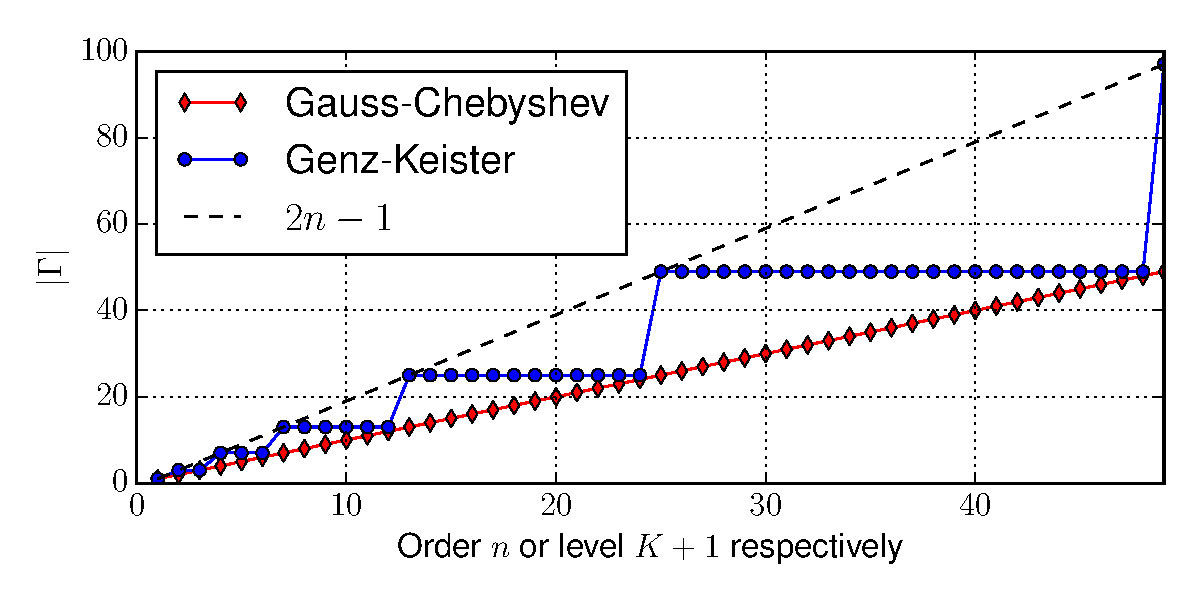
\includegraphics[width=\linewidth]{./img/number_nodes_chebyshevt.pdf}
  \caption{Number of nodes for the one-dimensional Gauss-Chebyshev and Genz-Keister quadrature
  rules of order $n$ or level $K$ respectively.}
  \label{fig:number_nodes_chebyshevt}
\end{figure}

\begin{figure}
  \centering
  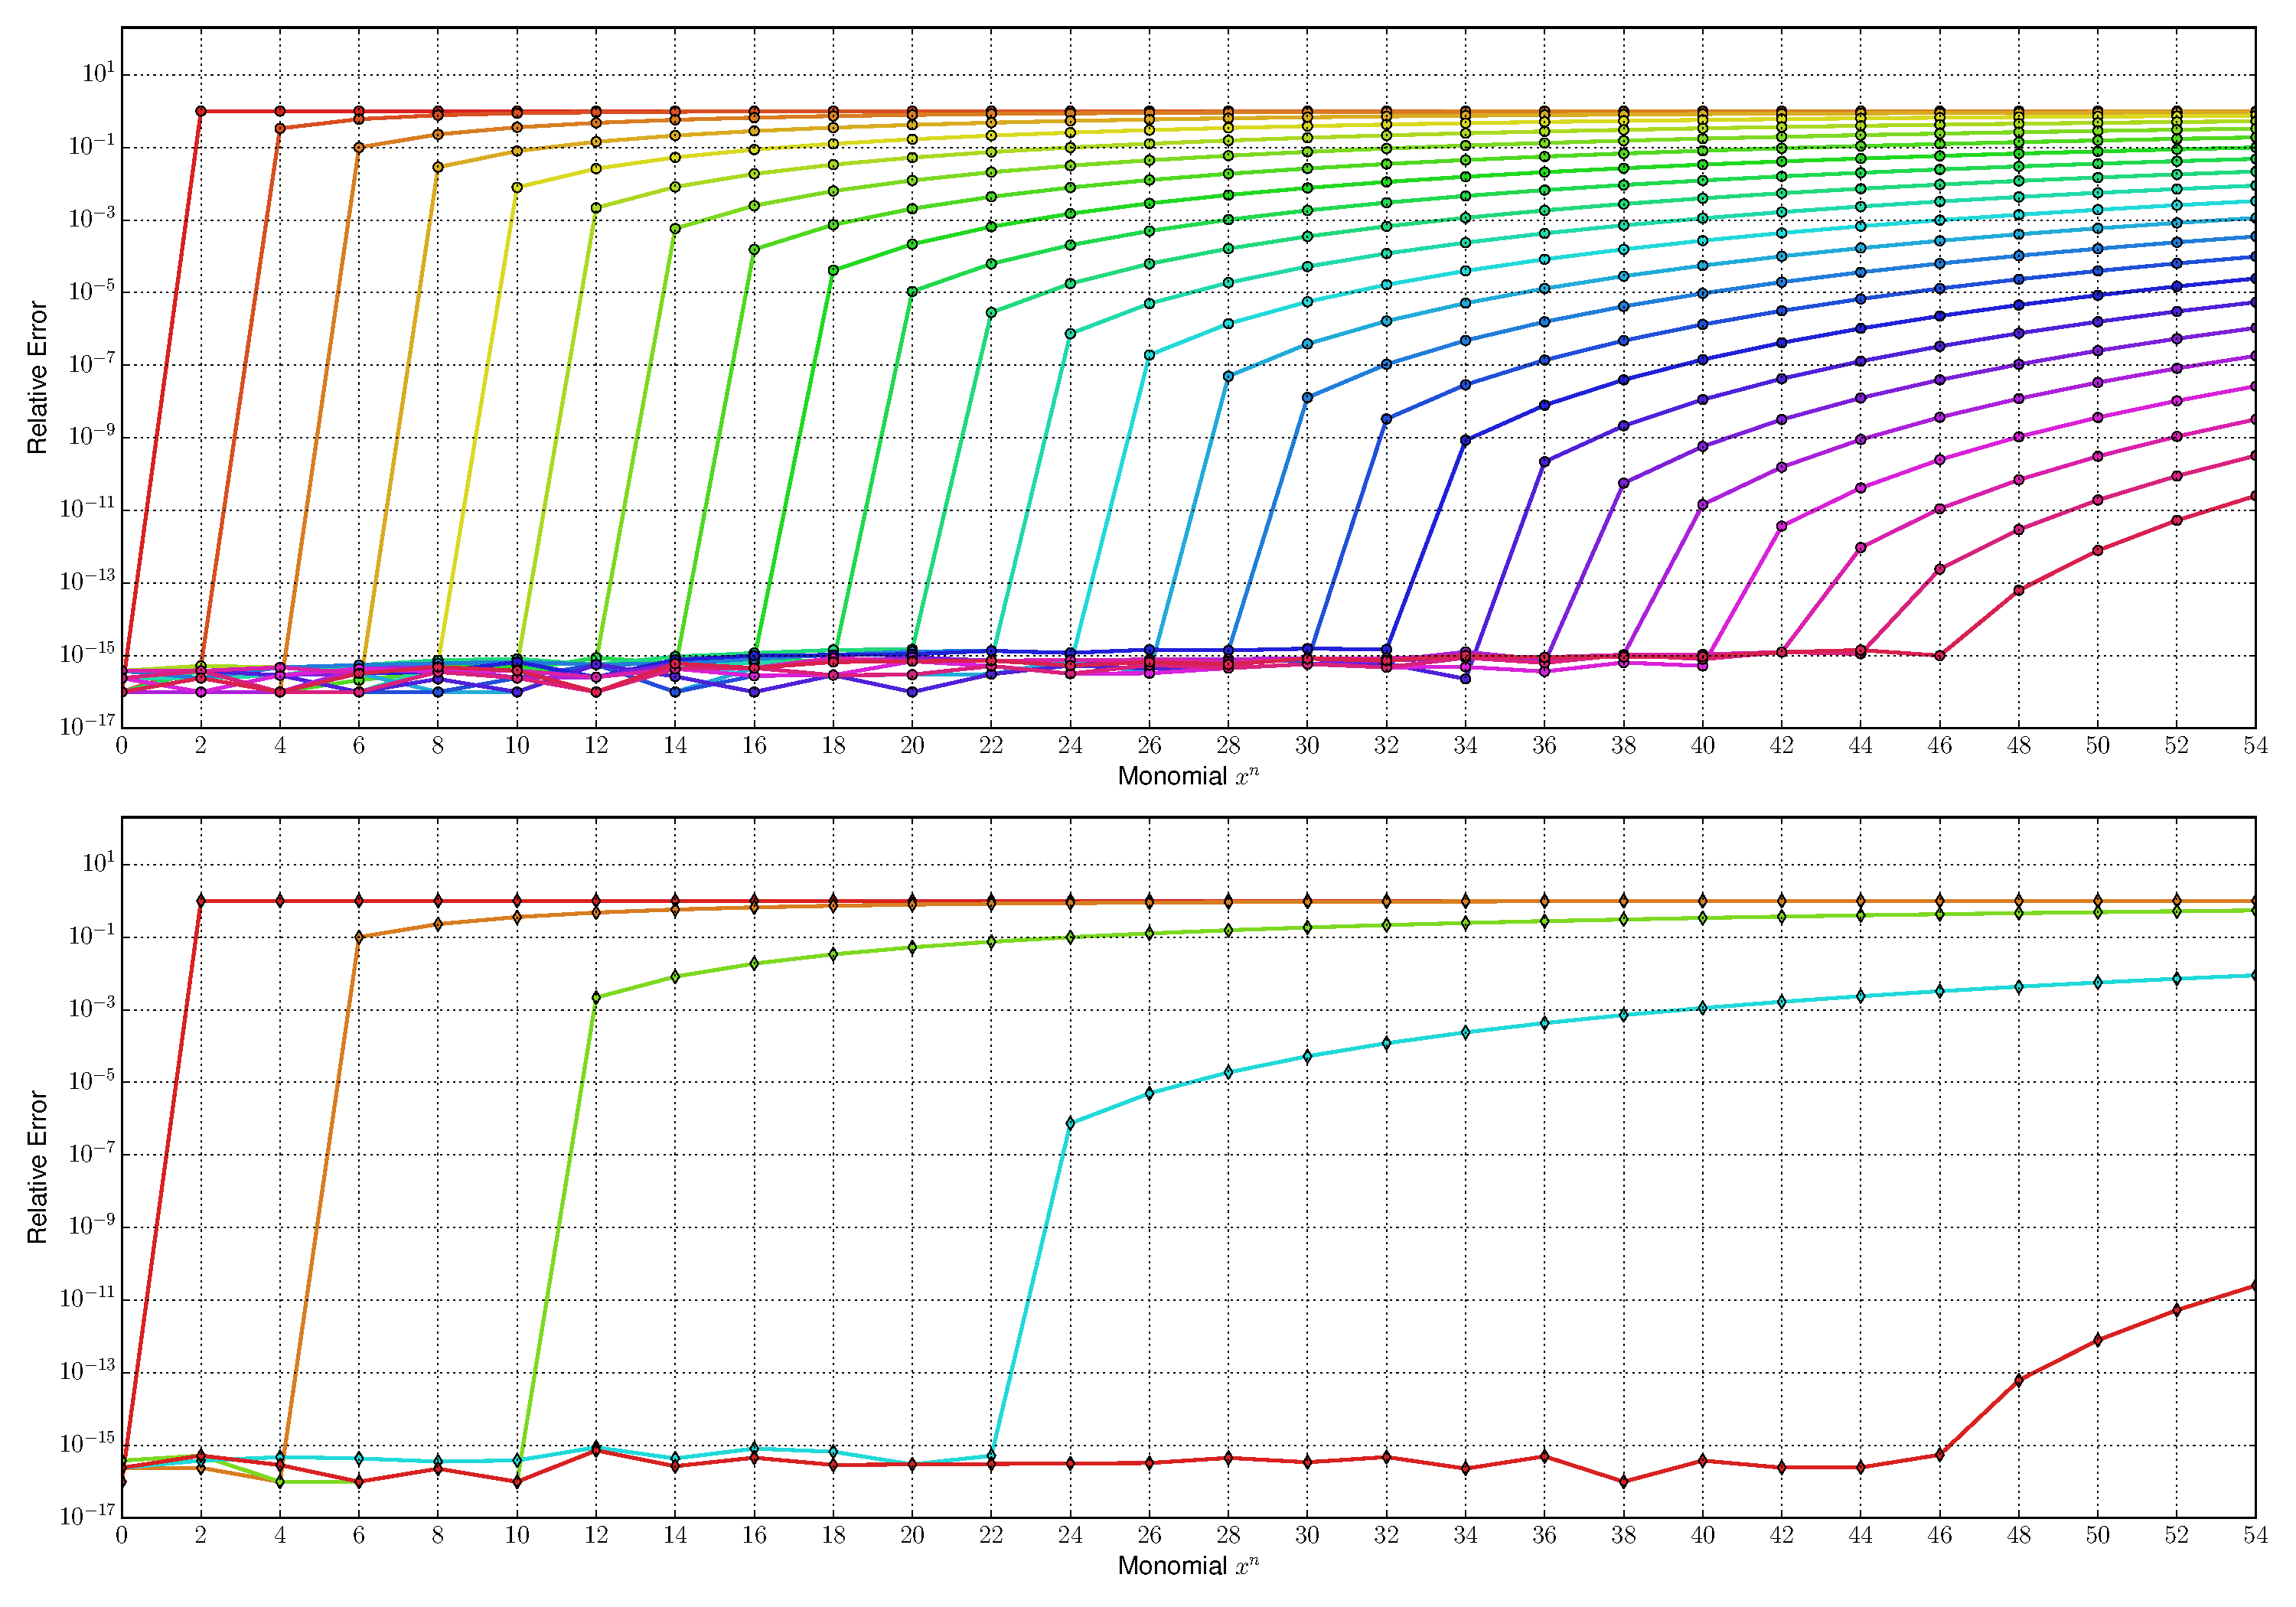
\includegraphics[width=\linewidth]{./img/monomial_errors_chebyshevt.pdf}
  \caption{Relative quadrature error for integration of single univariate monomials $x^n$ of increasing degree $n$.
  Each line represents a quadrature rule and the color indicates the number of nodes (colors wrap around once though).
  The upper plot shows Gauss-Chebyshev rules as reference while the lower one shows the Genz-Keister rules.
  The number of nodes for each of these rules is:
  $1$, $3$,  $7$, $13$, $25$ and the orders according to \eqref{eq:gk_rul_order} are:
  $1$, $5$, $11$, $23$, $47$ which perfectly agrees with the figure.
  All rules examined here are very stable up to machine precision.}
  \label{fig:monomial_errors_chebyshevt}
\end{figure}

\begin{figure}[h]
  \centering
  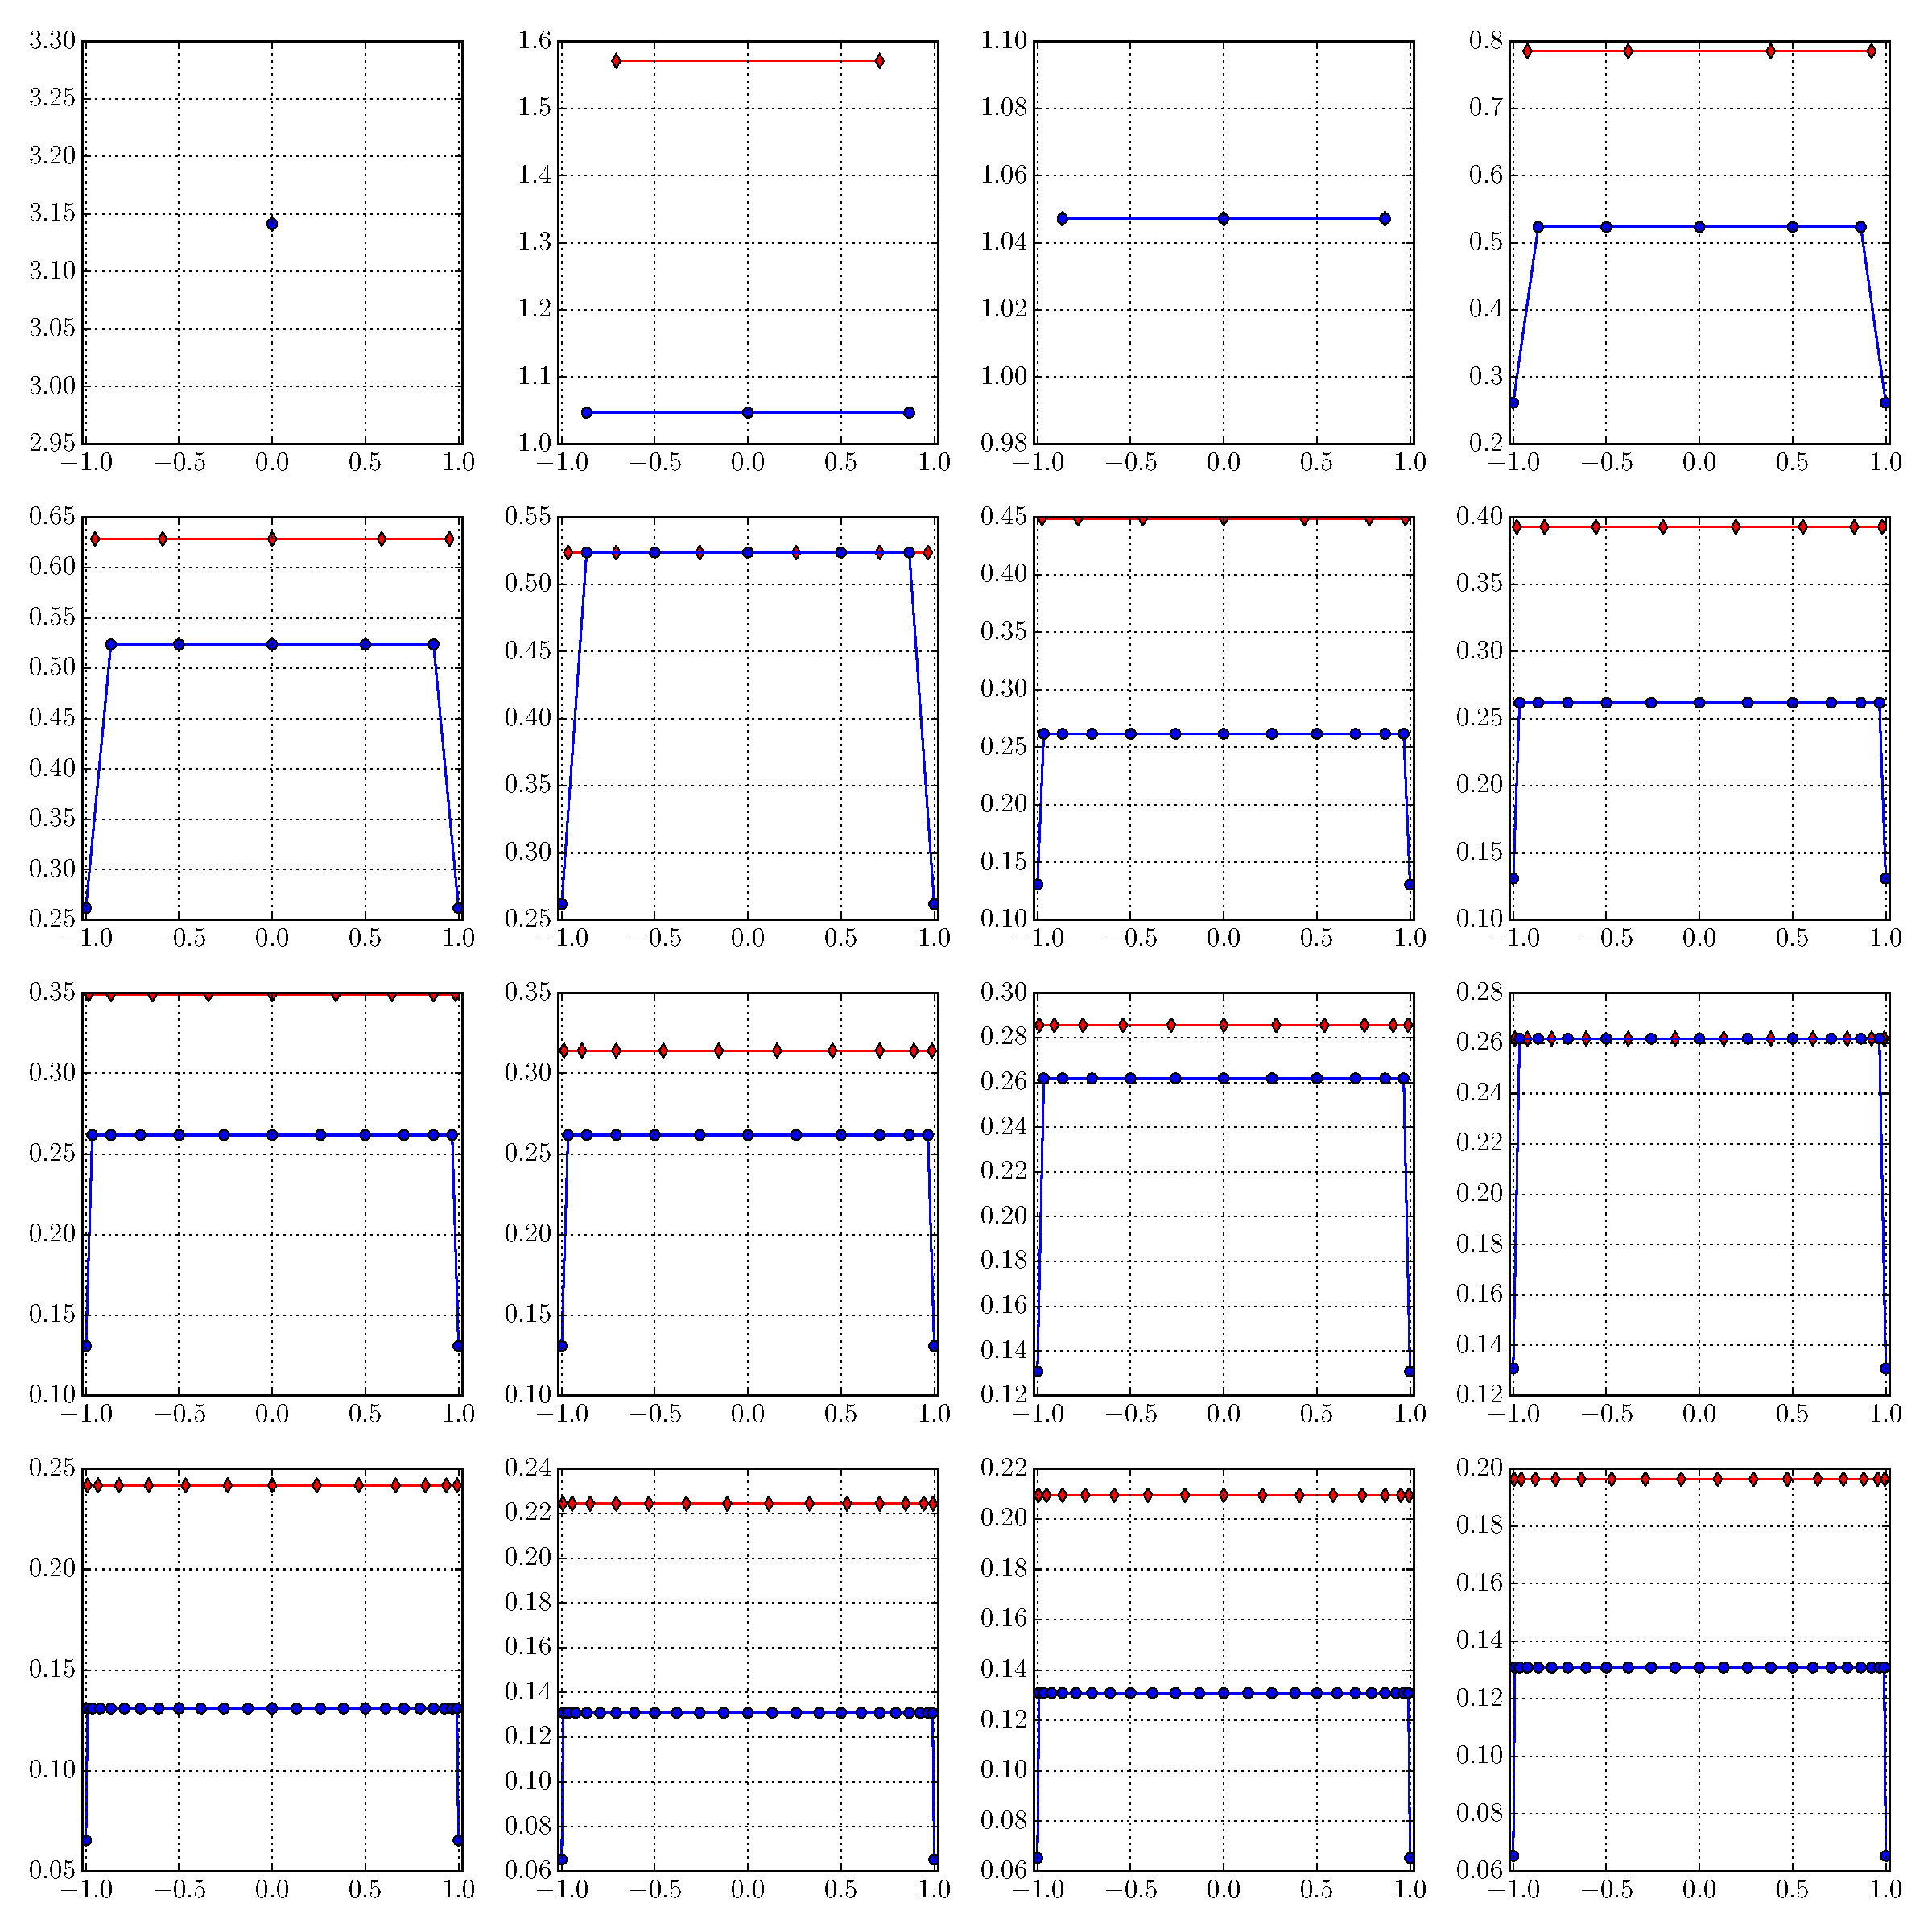
\includegraphics[width=\linewidth]{./img/gk_chebyshevt_nodes_1d.pdf}
  \caption{Gauss-Chebyshev (red) and Genz-Keister (blue) nodes versus
  corresponding weights. The 1- and 3-point rules are identical.}
  \label{fig:gk_chebyshevt_nodes_1d}
\end{figure}

\begin{figure}[h]
  \centering
  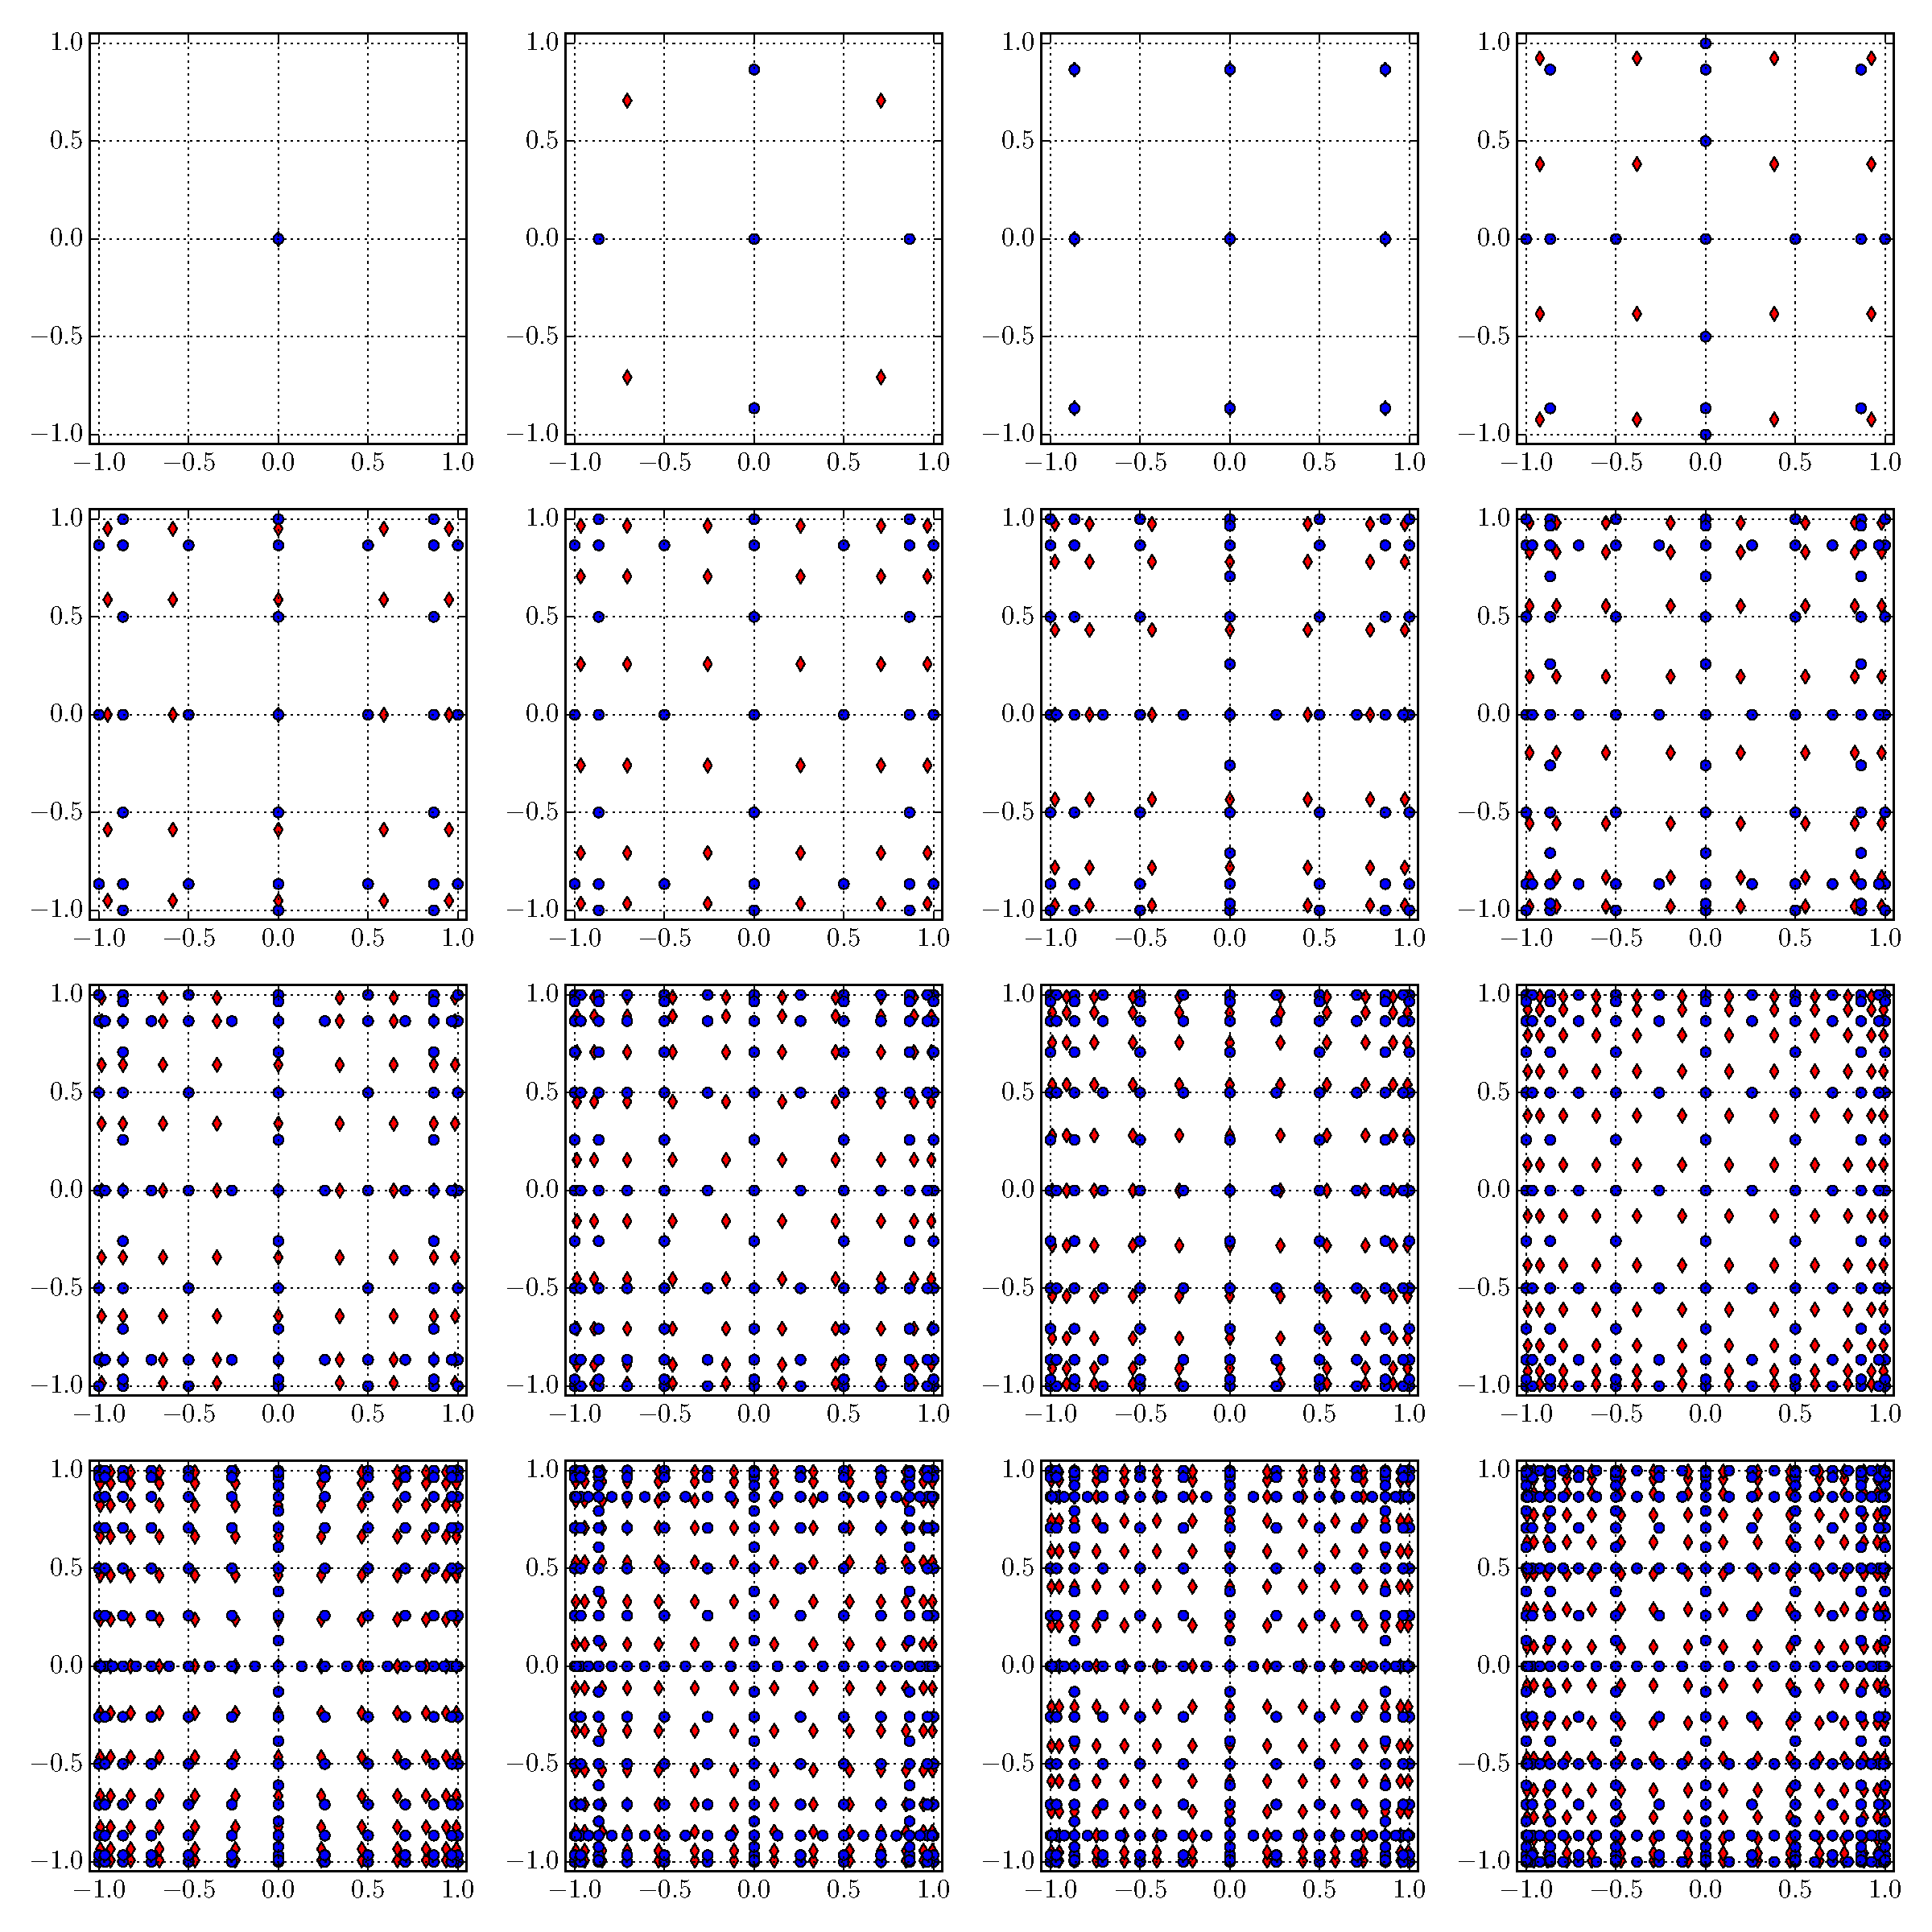
\includegraphics[width=\linewidth]{./img/gk_chebyshevt_nodes_2d.pdf}
  \caption{Gauss-Chebyshev (red) and Genz-Keister (blue) nodes for
  two-dimensional rules. The Gauss-Chebyshev points form a full tensor
  product.}
  \label{fig:gk_chebyshevt_nodes_2d}
\end{figure}

\begin{figure}
  \centering
  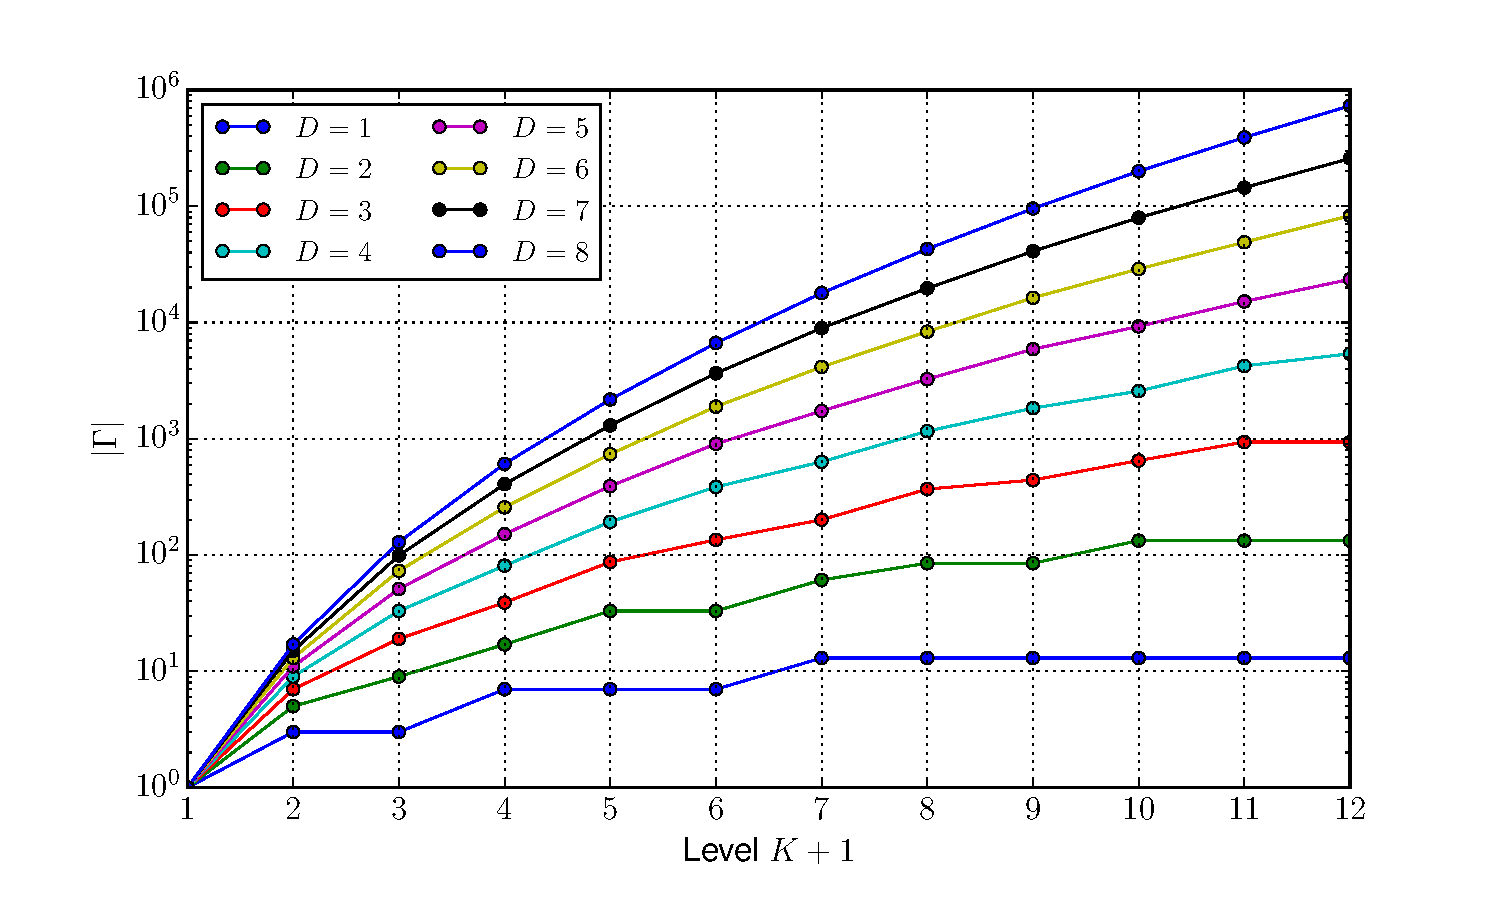
\includegraphics[width=\linewidth]{./img/number_nodes_levdim_chebyshevt.pdf}
  \caption{Number $|\Gamma|$ of Genz-Keister quadrature nodes for various levels $K$ and dimensions $D$.}
  \label{fig:number_nodes_levdim_chebyshevt}
\end{figure}

\begin{figure}[h]
  \centering
  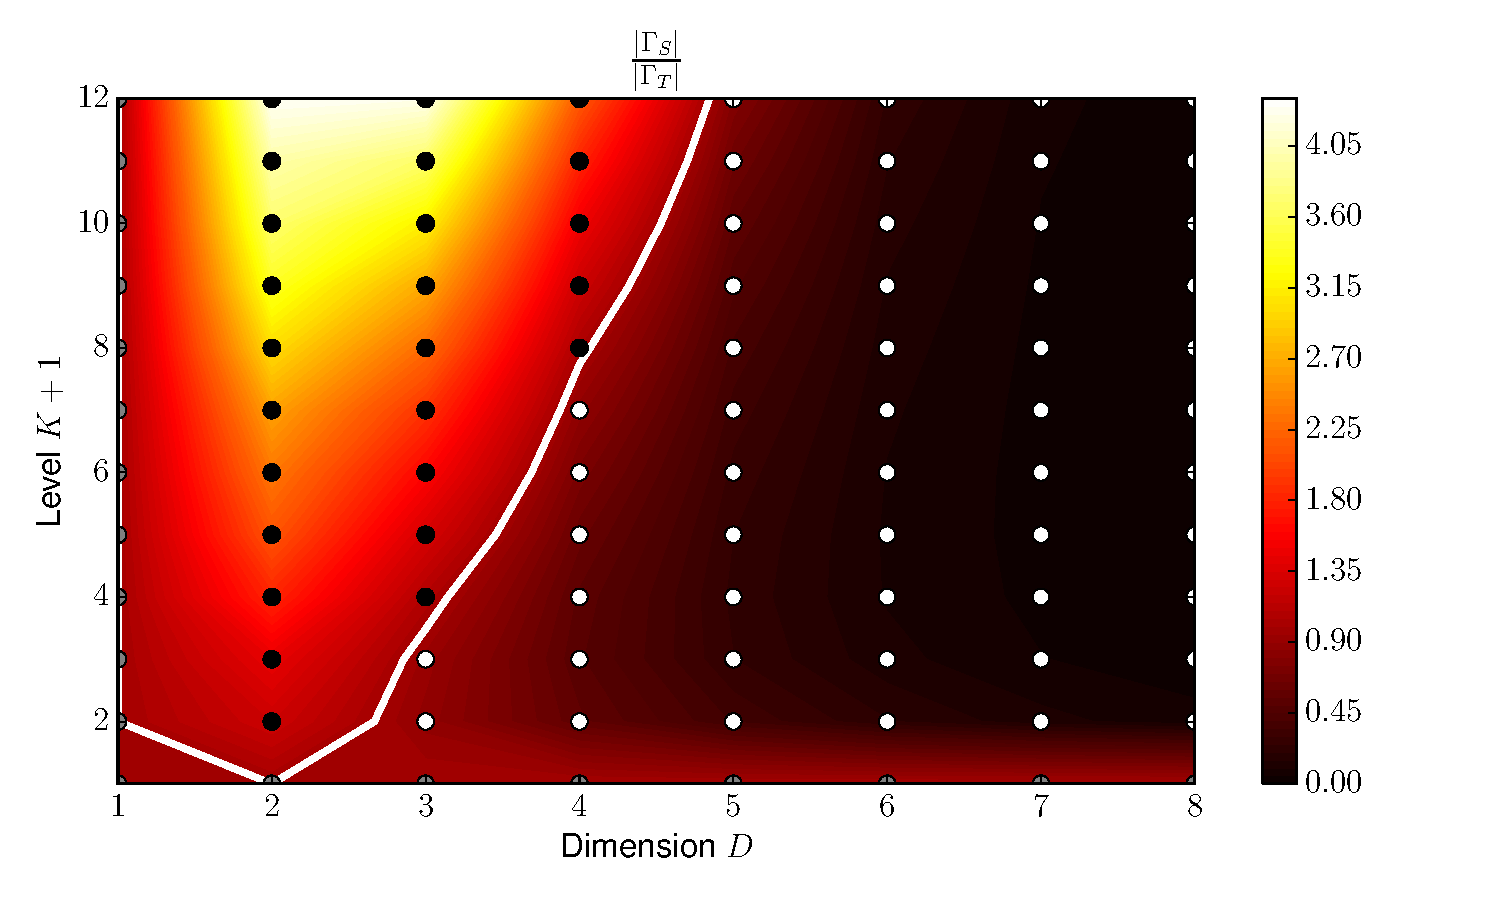
\includegraphics[width=0.8\linewidth]{./img/smol_chebyshevt_ratio.pdf}
  \caption{Ratio of the number of Gauss-Chebyshev quadrature points obtained
  via tensor product and classical Smolyak construction. White dots are $D,K$
  combinations where Genz-Keister is advantageous, while for black dots
  Genz-Keister is worse and for gray dots the ratio equals 1.}
  \label{fig:smol_chebyshevt_ratio}
\end{figure}

\begin{figure}[h]
  \centering
  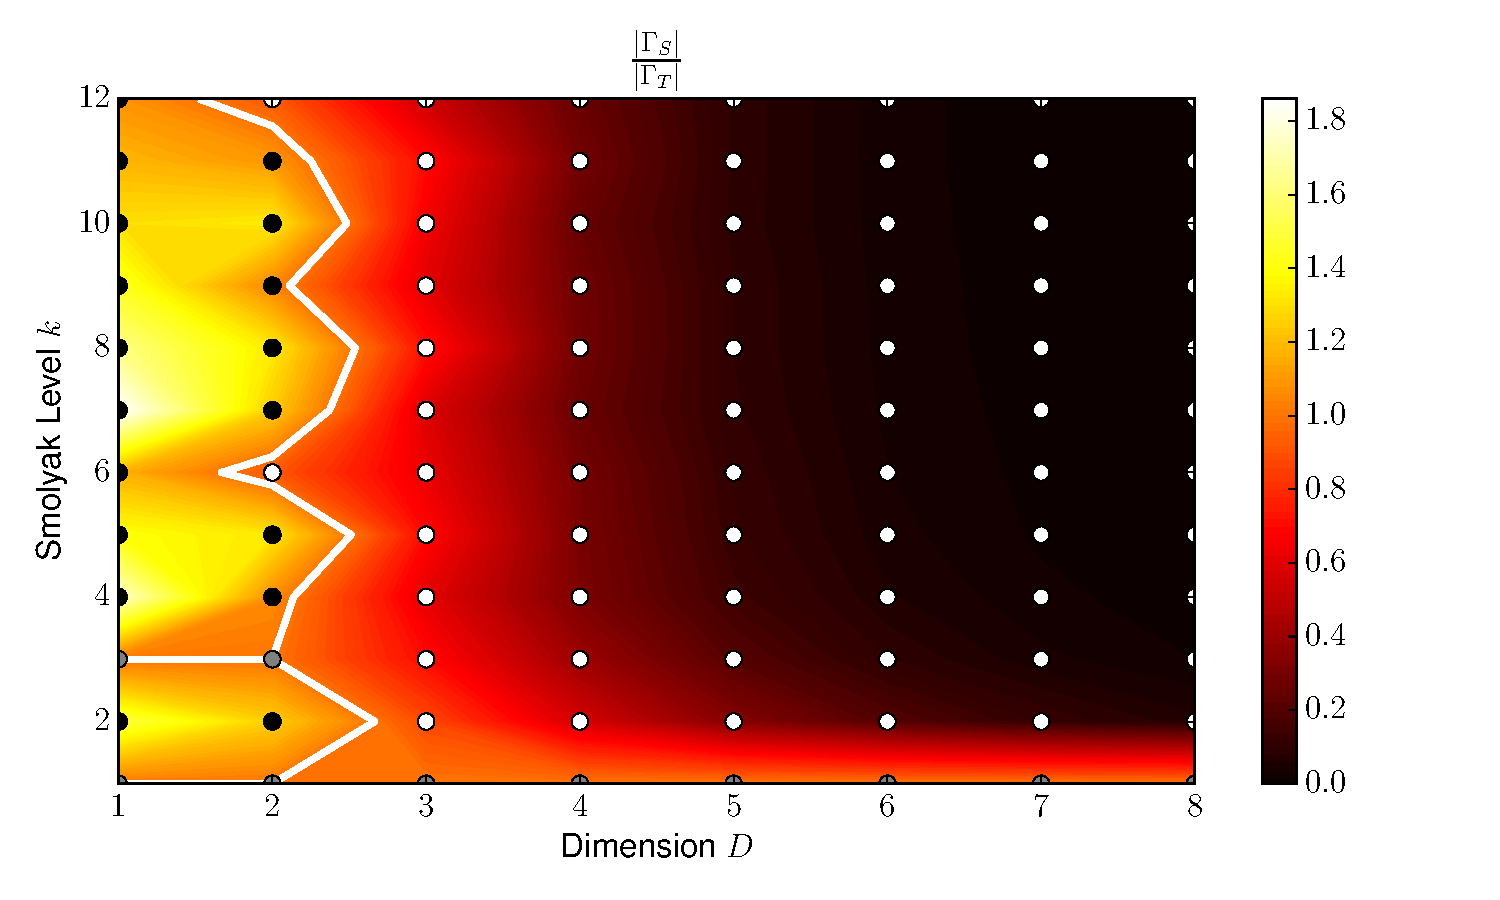
\includegraphics[width=0.8\linewidth]{./img/gk_chebyshevt_ratio.pdf}
  \caption{Ratio of the number of Genz-Keister and Gauss-Chebyshev tensor product
  points for dimensions $D$ up to 8 and Level $K \leq 12$. White dots are $D,K$
  combinations where Genz-Keister is advantageous, while for black dots
  Genz-Keister is worse and for gray dots the ratio equals 1.}
  \label{fig:gk_chebyshevt_ratio}
\end{figure}

\begin{figure}[h]
  \centering
  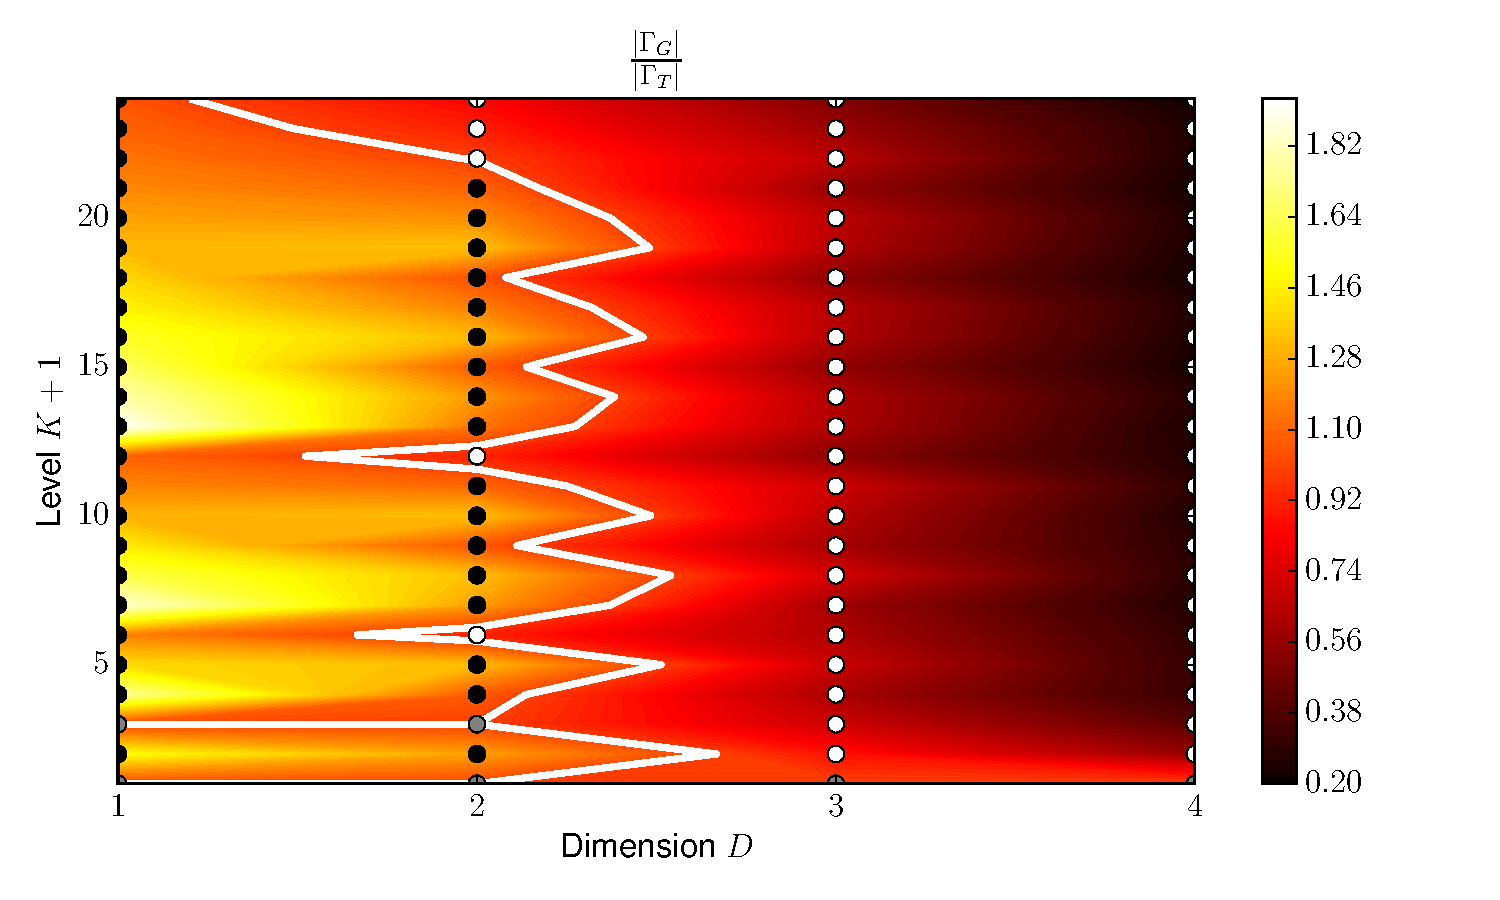
\includegraphics[width=0.8\linewidth]{./img/gk_chebyshevt_ratio_large.pdf}
  \caption{Ratio of the number of Genz-Keister and Gauss-Chebyshev tensor product
  points for dimensions 1 to 4 and Level $K \leq 24$. White dots are $D,K$
  combinations where Genz-Keister is advantageous, while for black dots
  Genz-Keister is worse and for gray dots the ratio equals 1.}
  \label{fig:gk_chebyshevt_ratio_large}
\end{figure}

\begin{figure}[h]
  \centering
  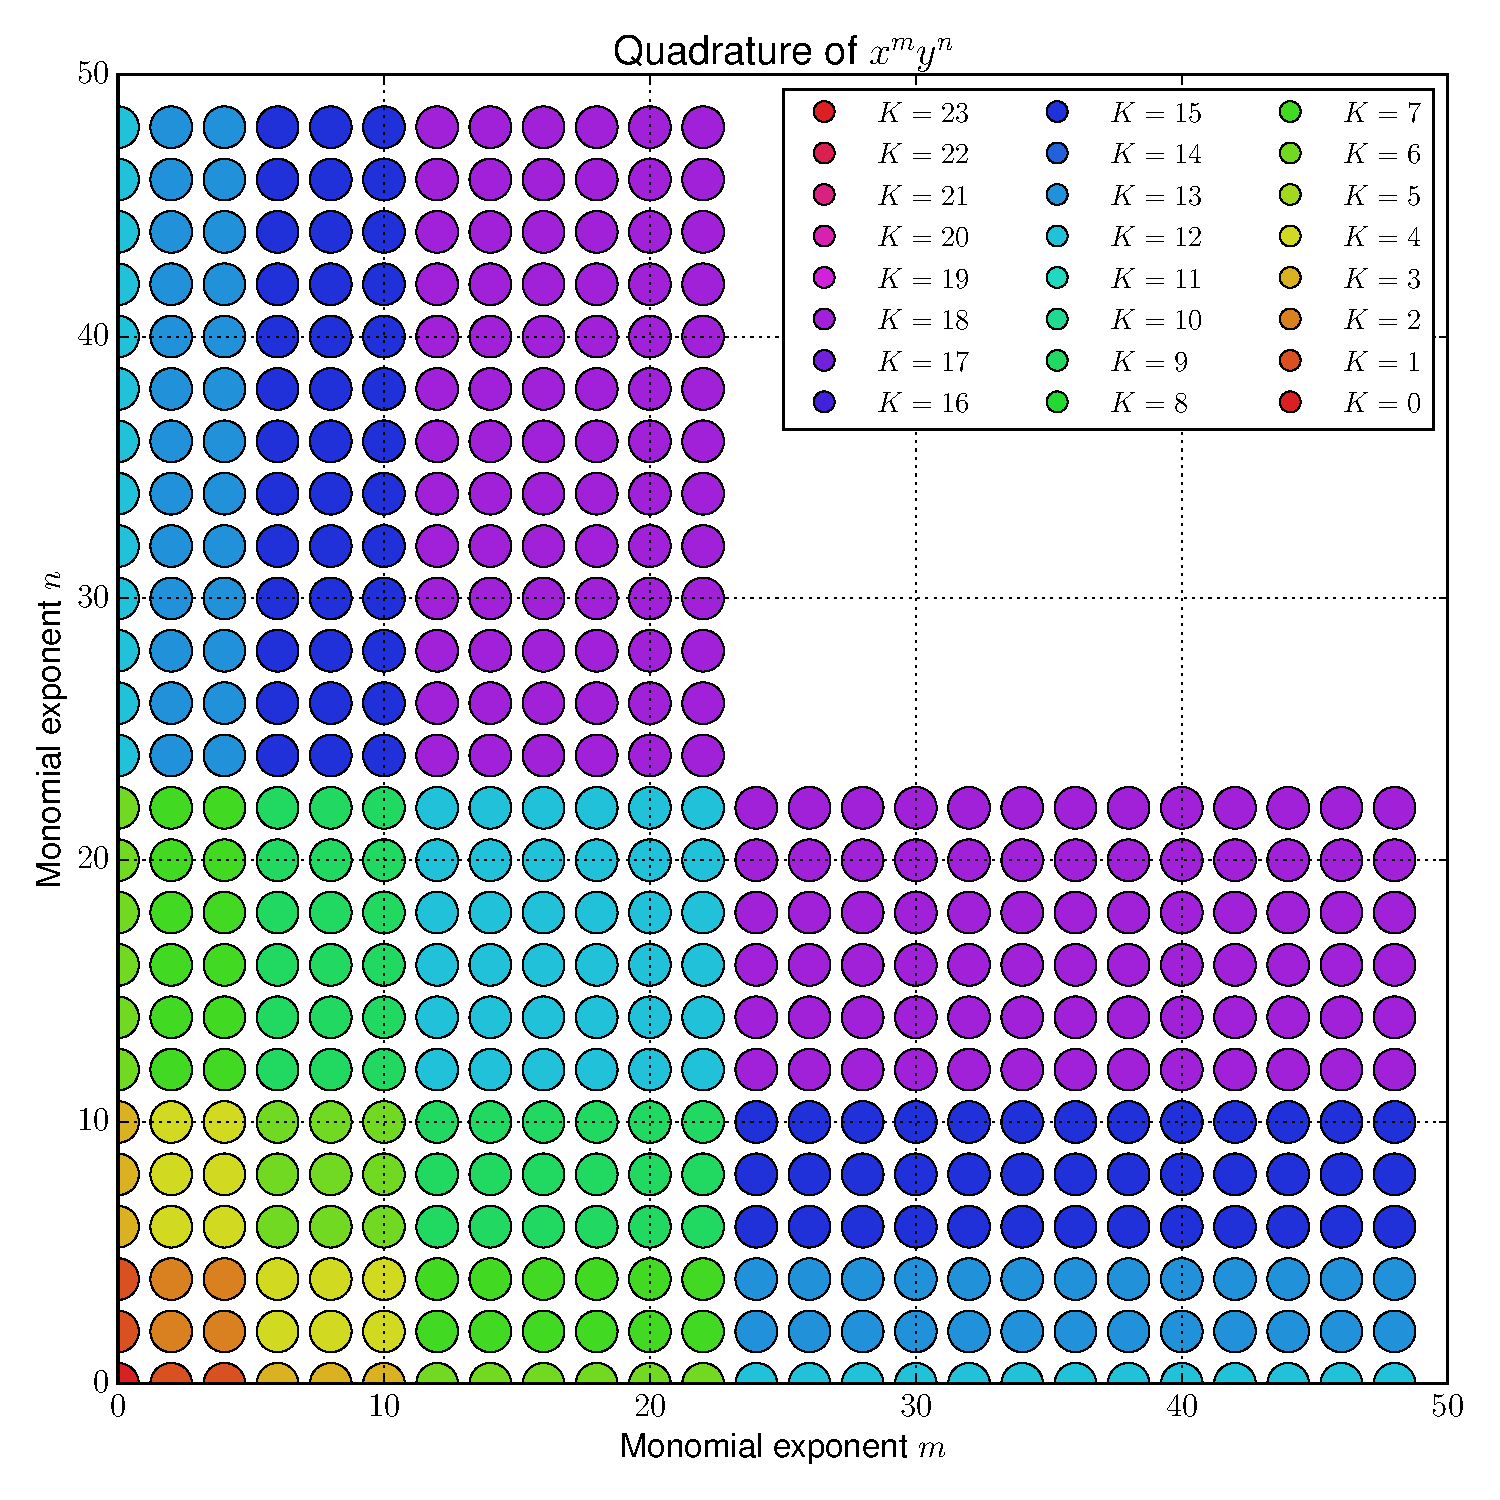
\includegraphics[width=\linewidth]{./img/monomial_errors_chebyshevt_2D.pdf}
  \caption{Quadrature of the bivariate monomials $x^m y^n$ for $0 \leq n, m \leq 50$.
  Each pair $(m,n)$ is color-coded by the lowest level $K$ rule that correctly
  integrates the monomial with a relative error not larger than $10^{-13}$.}
  \label{fig:monomial_errors_chebyshevt_2D}
\end{figure}

For testing the quadrature rules in $D$ dimensions, the following integral
over multi-variate monomials with $\vec{n} \in \mathbb{N}_0^D$ is used:
\begin{equation} \label{eq:chebyshevt_exact_solution}
  \idotsint \limits_{\vec{x} \in [-1,1]^D} \prod_{d=1}^D x_d^{n_d} \frac{1}{\sqrt{1-x_d^2}} \di{\vec{x}}
  =
  \left(\frac{\sqrt{\pi}}{2}\right)^D
  \prod_{d=1}^D \left(1 + (-1)^{n_d}\right)
  \frac{\Gamma\left(\frac{n_d}{2}+\frac{1}{2}\right)}
       {\Gamma\left(\frac{n_d}{2}+1\right)}
\end{equation}
where we know the exact solution in closed form.

\begin{subfigures}
  \label{fig:monomial_errors_chebyshevt_multivariate}
  \begin{figure}\centering
    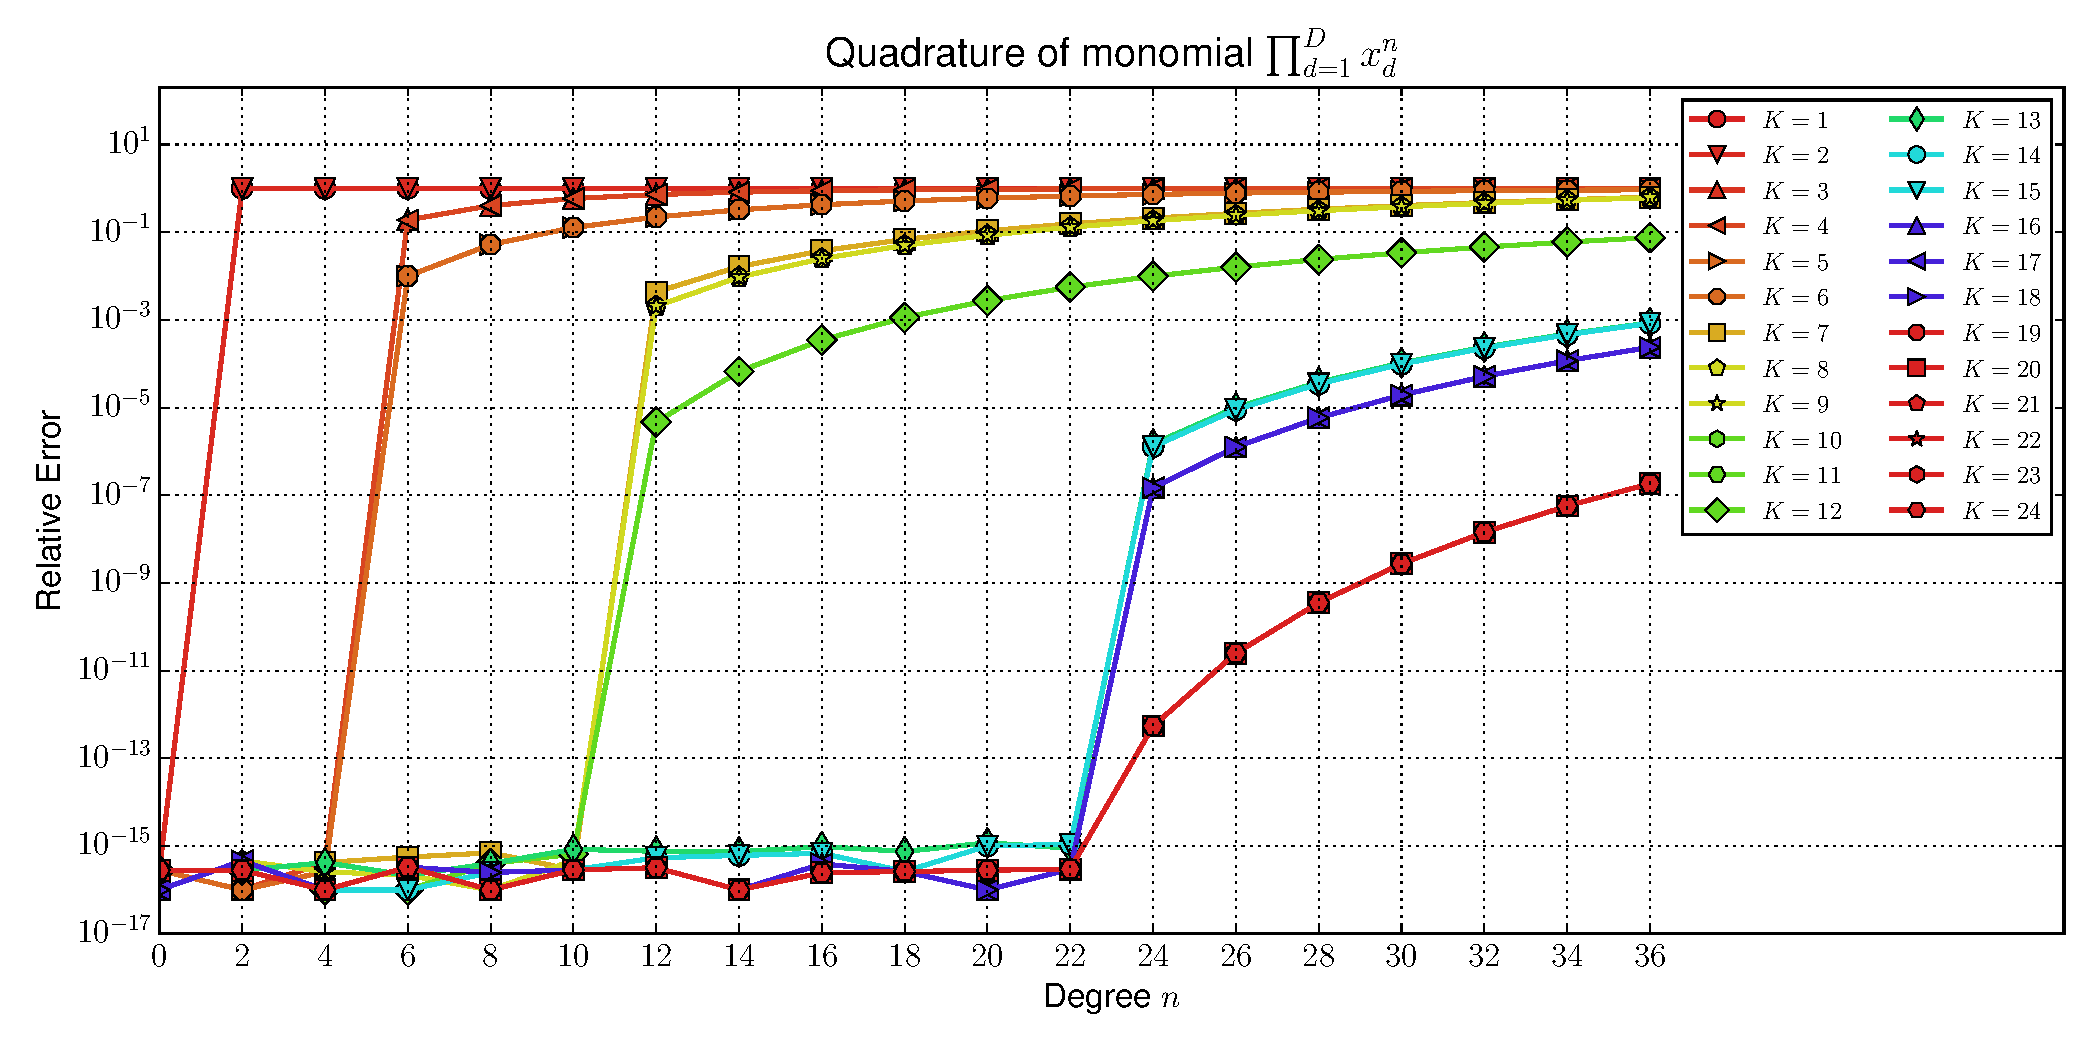
\includegraphics[width=\linewidth]{./img/monomial_errors_chebyshevt_multivariate_dimension_2.pdf}
    \caption{Relative errors for the integral \eqref{eq:chebyshevt_exact_solution}
    in $D=2$ dimensions. All variables $x_d$ share the same exponent $n$.}
    \label{fig:monomial_errors_chebyshevt_multivariate_dimension_2}
  \end{figure}
  \begin{figure}\centering
    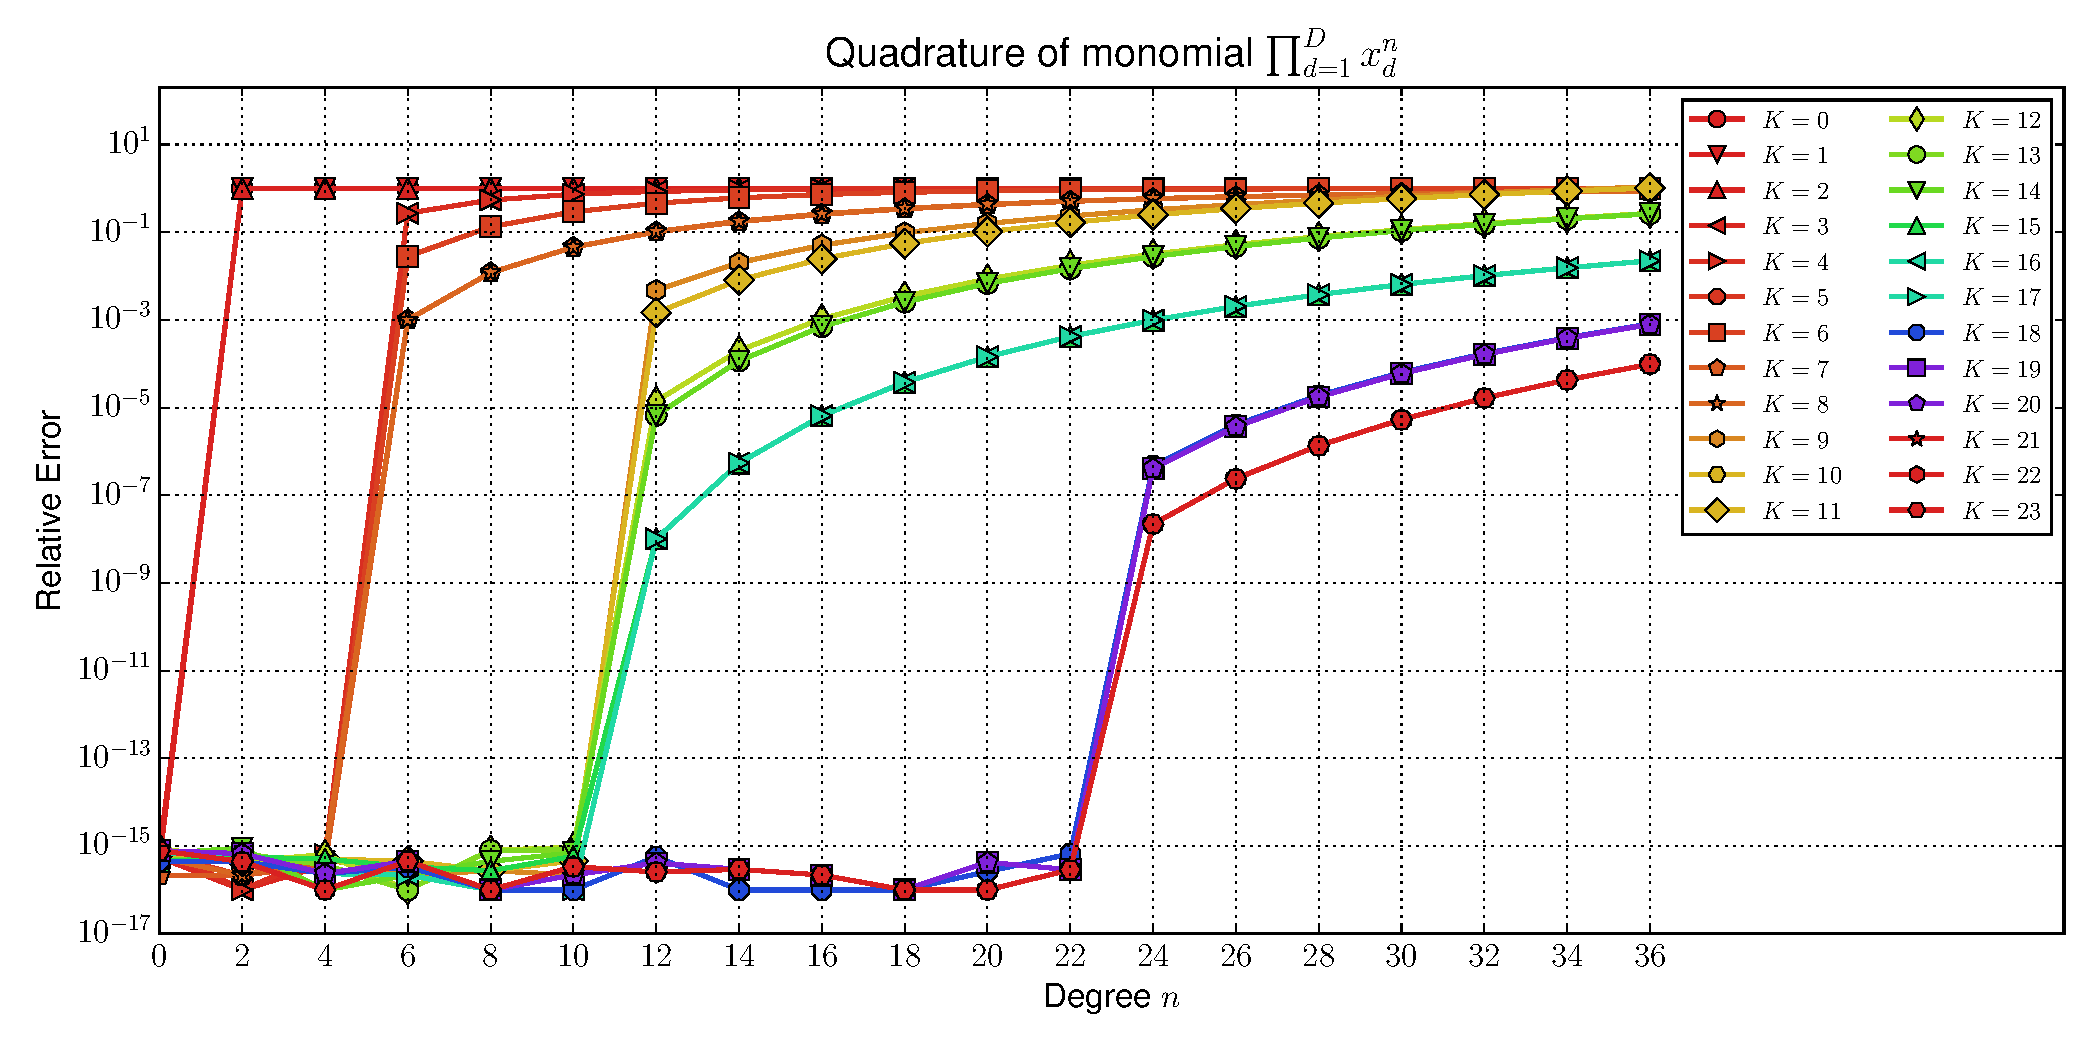
\includegraphics[width=\linewidth]{./img/monomial_errors_chebyshevt_multivariate_dimension_3.pdf}
    \caption{Relative errors for the integral \eqref{eq:chebyshevt_exact_solution}
    in $D=3$ dimensions. All variables $x_d$ share the same exponent $n$.}
    \label{fig:monomial_errors_chebyshevt_multivariate_dimension_3}
  \end{figure}
  \begin{figure}\centering
    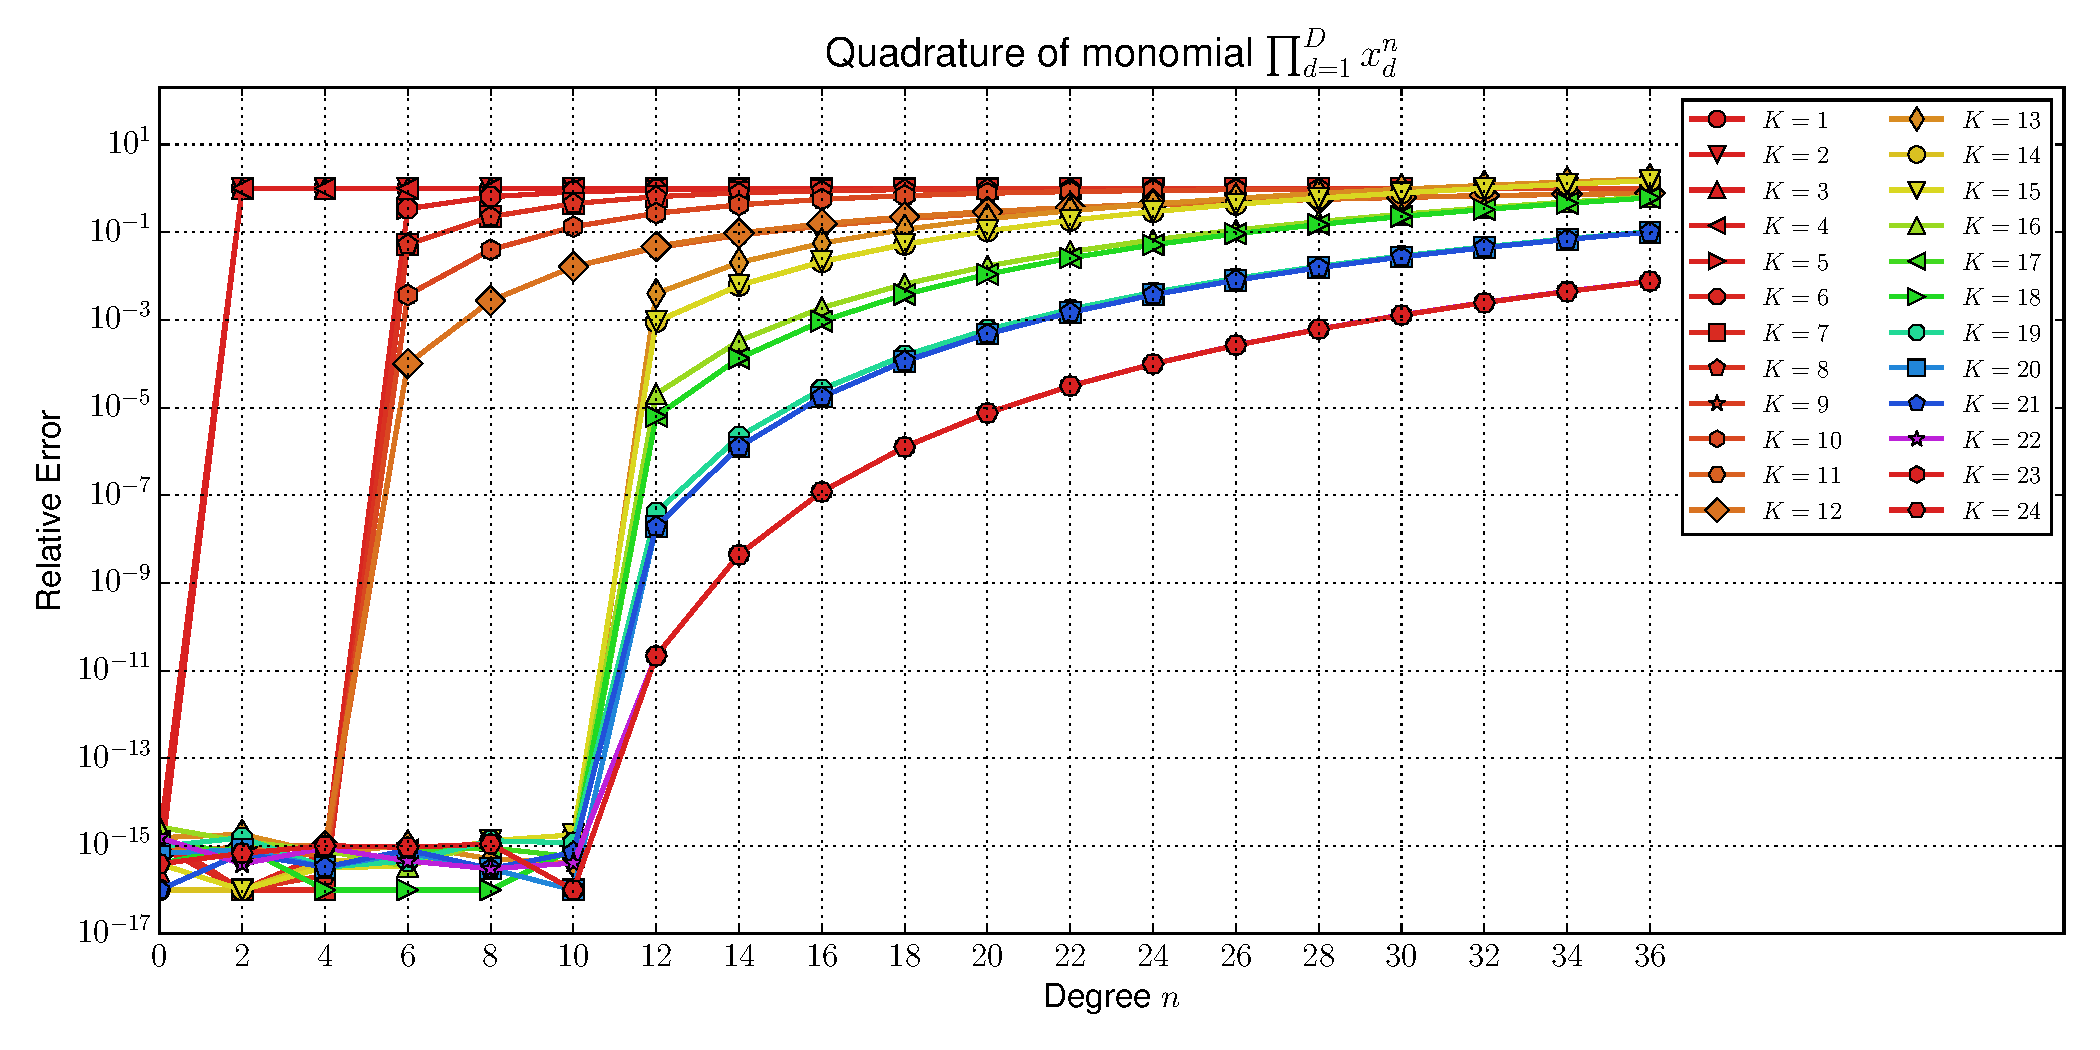
\includegraphics[width=\linewidth]{./img/monomial_errors_chebyshevt_multivariate_dimension_4.pdf}
    \caption{Relative errors for the integral \eqref{eq:chebyshevt_exact_solution}
    in $D=4$ dimensions. All variables $x_d$ share the same exponent $n$.}
    \label{fig:monomial_errors_chebyshevt_multivariate_dimension_4}
  \end{figure}
  \begin{figure}\centering
    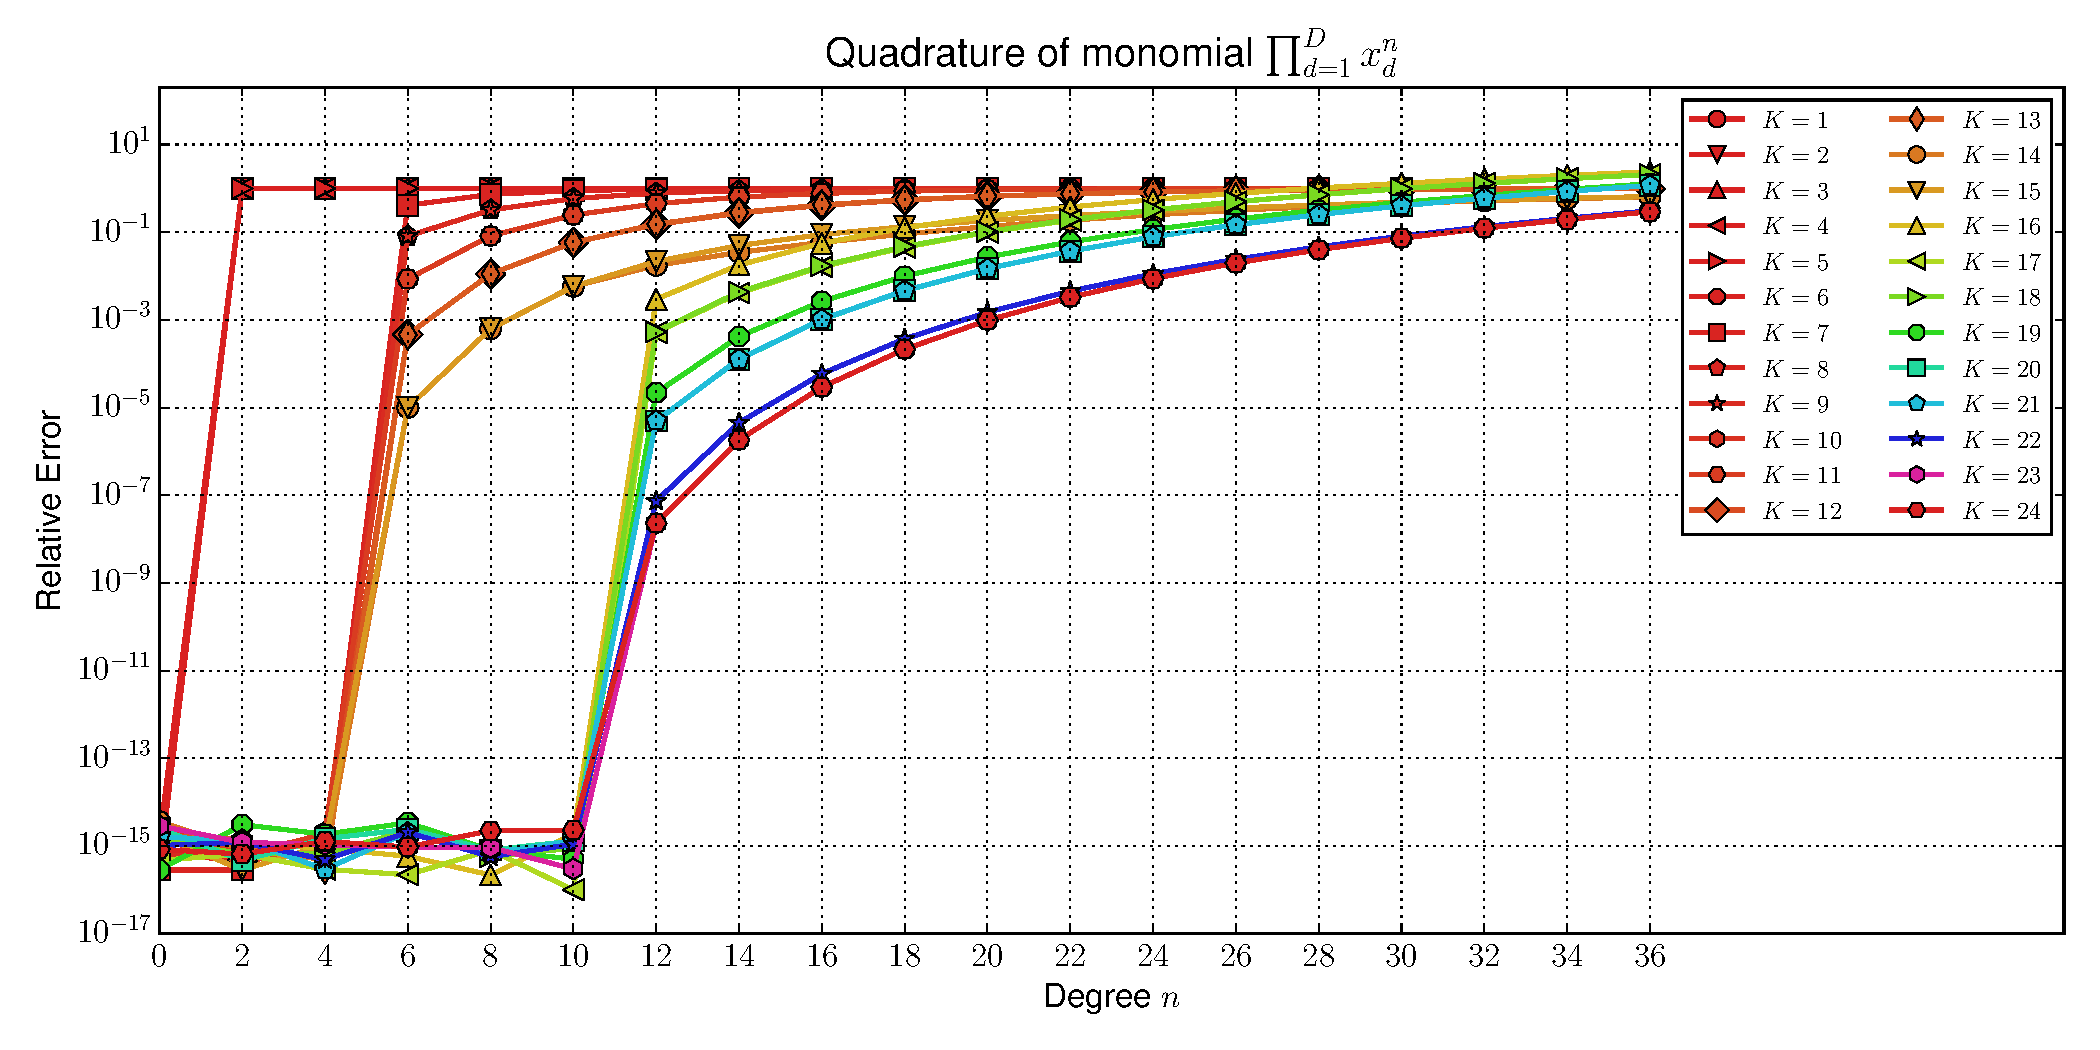
\includegraphics[width=\linewidth]{./img/monomial_errors_chebyshevt_multivariate_dimension_5.pdf}
    \caption{Relative errors for the integral \eqref{eq:chebyshevt_exact_solution}
    in $D=5$ dimensions. All variables $x_d$ share the same exponent $n$.}
    \label{fig:monomial_errors_chebyshevt_multivariate_dimension_5}
  \end{figure}
  \begin{figure}\centering
    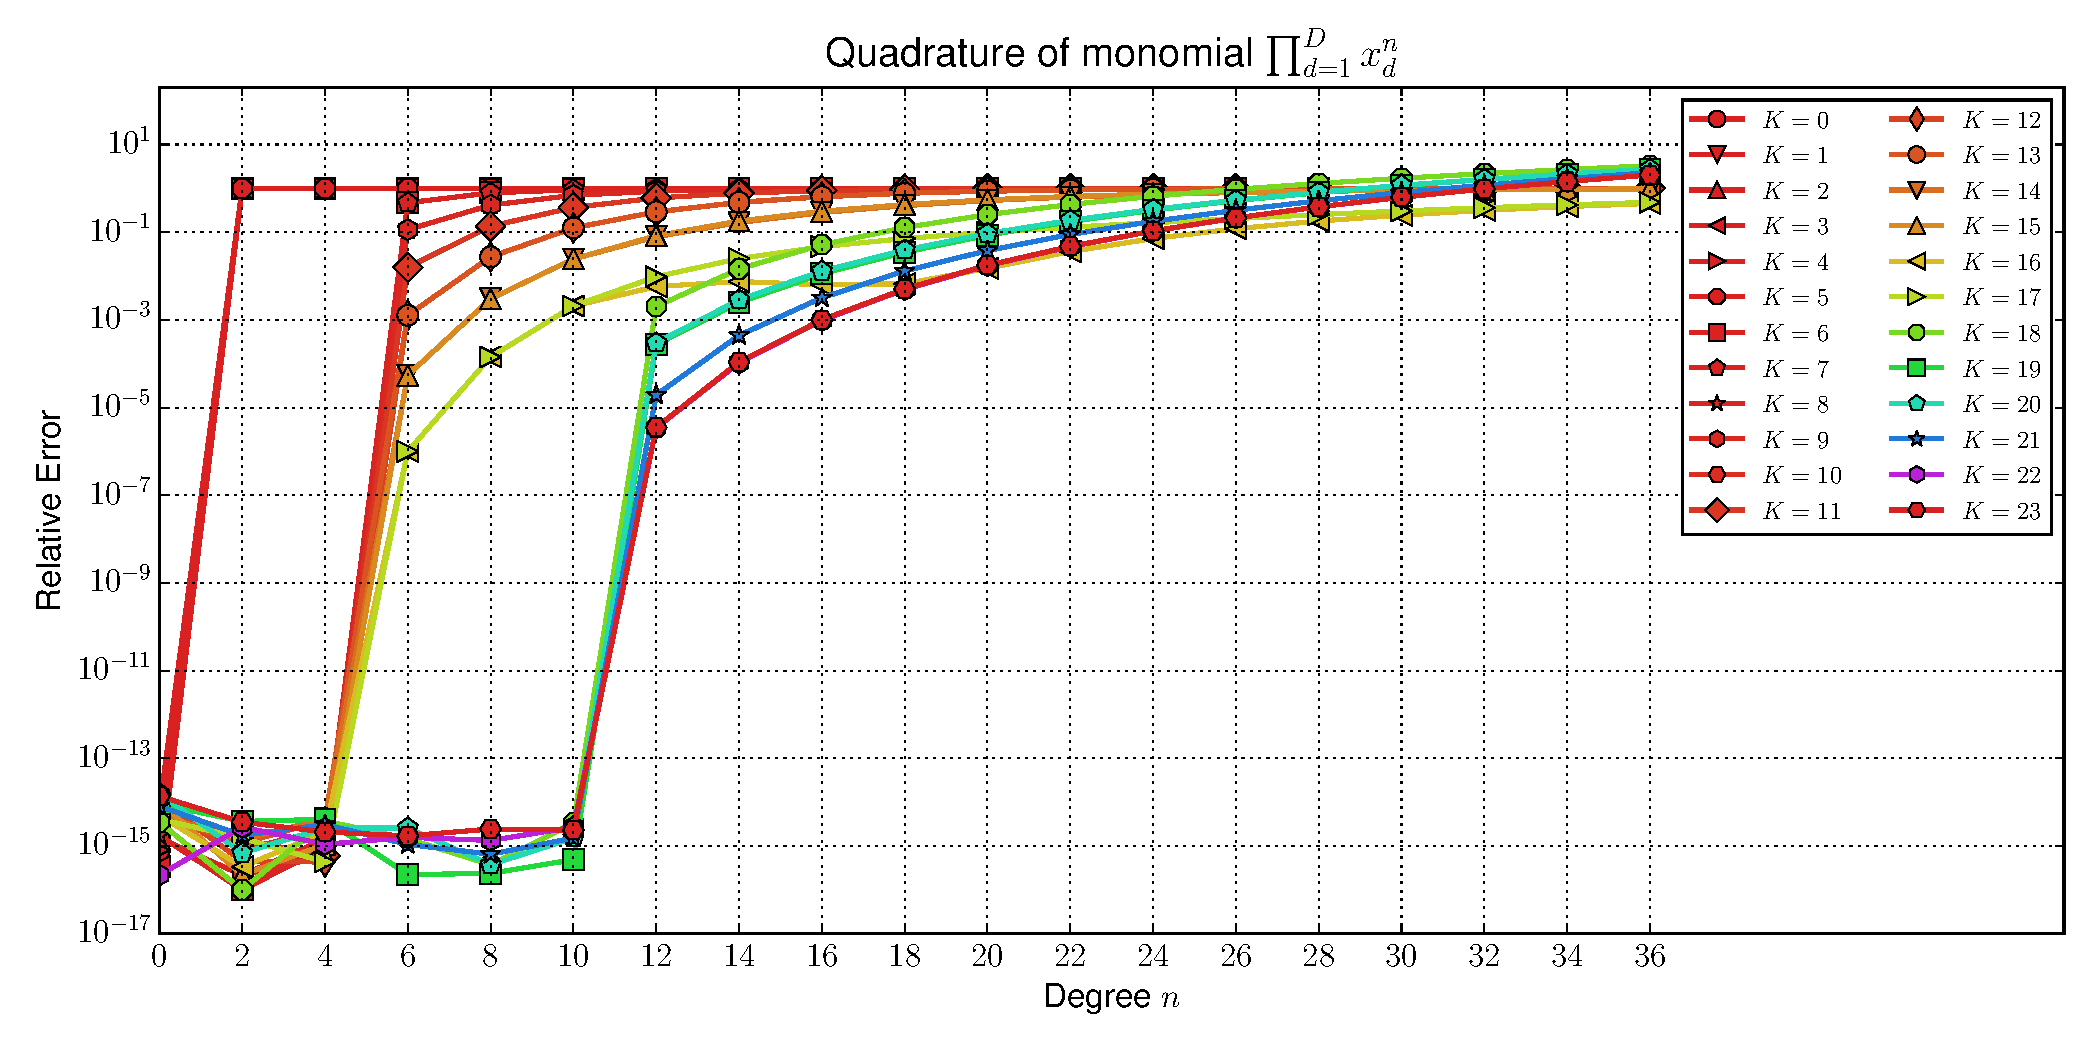
\includegraphics[width=\linewidth]{./img/monomial_errors_chebyshevt_multivariate_dimension_6.pdf}
    \caption{Relative errors for the integral \eqref{eq:chebyshevt_exact_solution}
    in $D=6$ dimensions. All variables $x_d$ share the same exponent $n$.}
    \label{fig:monomial_errors_chebyshevt_multivariate_dimension_6}
  \end{figure}
\end{subfigures}

\FloatBarrier
\subsection{Chebyshev Quadrature of the second kind}

For the second kind $U_n$ of Chebyshev polynomials we use
$\mathcal{K} = (1, 2, 4, 8, 16, 32)$ with the $\vec{z}$ sequence:
\begin{equation*}
  \vec{z} = (0, 0, 1, 0, 3, 2, 1, 0, 7, 6, 5, 4, 3, 2, 1, 0, 15, 14, 13, 12, 11,
             10, 9, 8, 7, 6, 5, 4, 3, 2, 1, 0, 1)\,.
\end{equation*}
Once more we could extend $\mathcal{K}$ by doubling the degree.
Using this extension we get the one-dimensional quadrature nodes and
weights shown in Figure \ref{fig:gk_chebyshevu_nodes_1d}.
Figure \ref{fig:gk_chebyshevu_nodes_2d} shows the sparse
node distribution in the plane for two-dimensional quadrature rules.
For $D = 2$ there are levels where Genz-Keister is better than
Gauss-Chebyshev tensor products but there are also levels where
it behaves the other way round. The details are shown in Figures
\ref{fig:gk_chebyshevu_ratio} and \ref{fig:gk_chebyshevu_ratio_large}.

\begin{figure}[h]
  \centering
  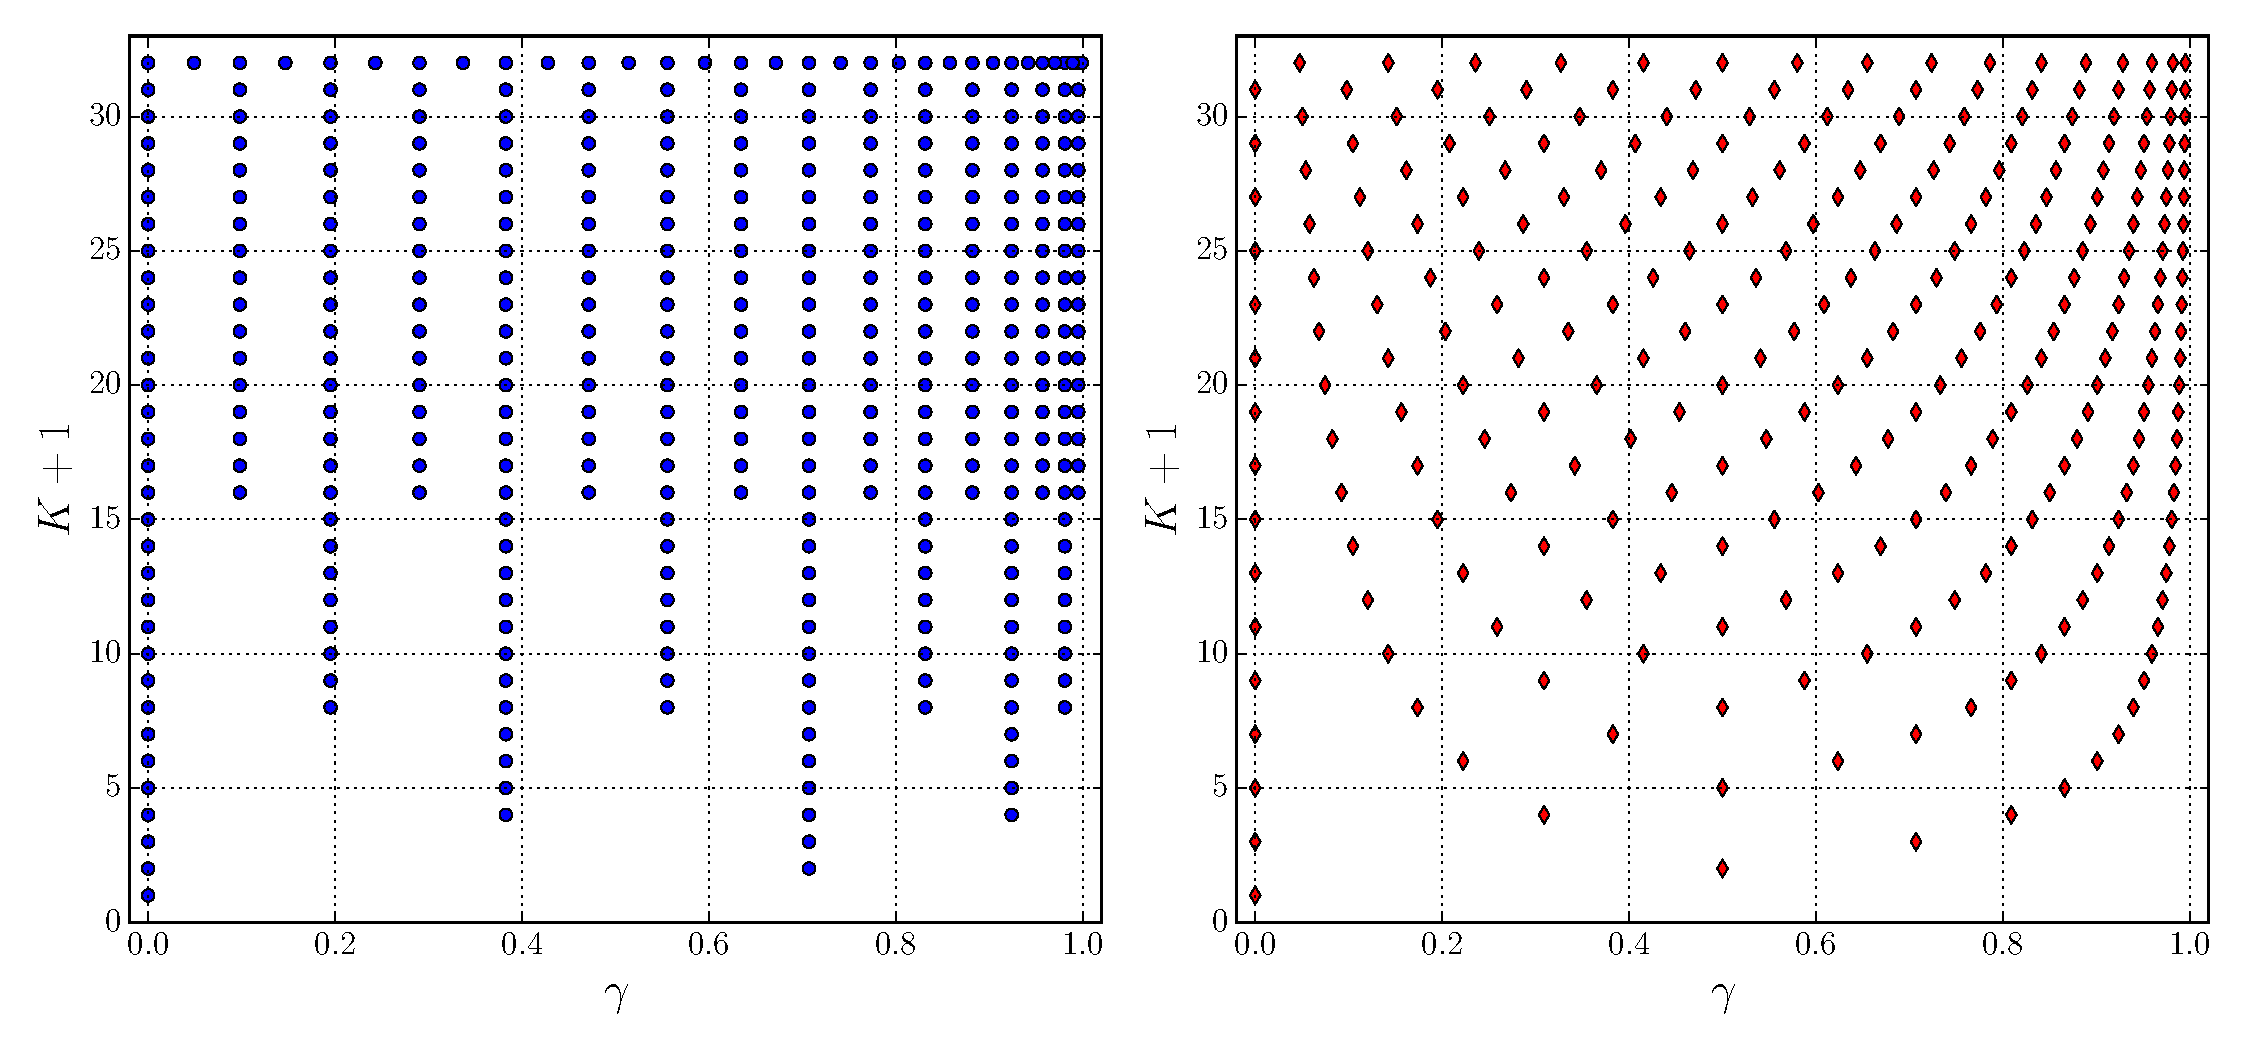
\includegraphics[width=\linewidth]{./img/gk_chebyshevu_nodes_cmp.pdf}
  \caption{Comparison of Gauss-Chebyshev nodes (right) and nested Genz-Keister nodes (left)
  based on the $\mathcal{K} = (1,2,4,8,16,32)$ Kronrod extension. The points are
  nicely nested and well suited for sparse grids.}
  \label{fig:gk_chebyshevu_nodes_cmp}
\end{figure}

\begin{figure}
  \centering
  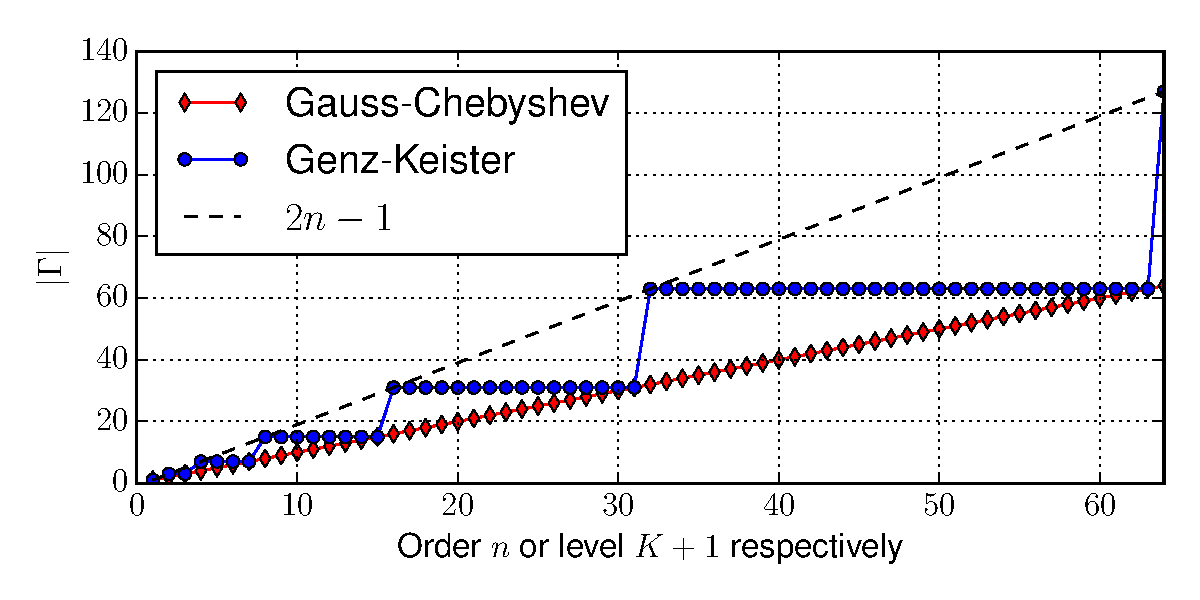
\includegraphics[width=\linewidth]{./img/number_nodes_chebyshevu.pdf}
  \caption{Number of nodes for the one-dimensional Gauss-Chebyshev and Genz-Keister quadrature
  rules of order $n$ or level $K$ respectively.}
  \label{fig:number_nodes_chebyshevu}
\end{figure}

\begin{figure}
  \centering
  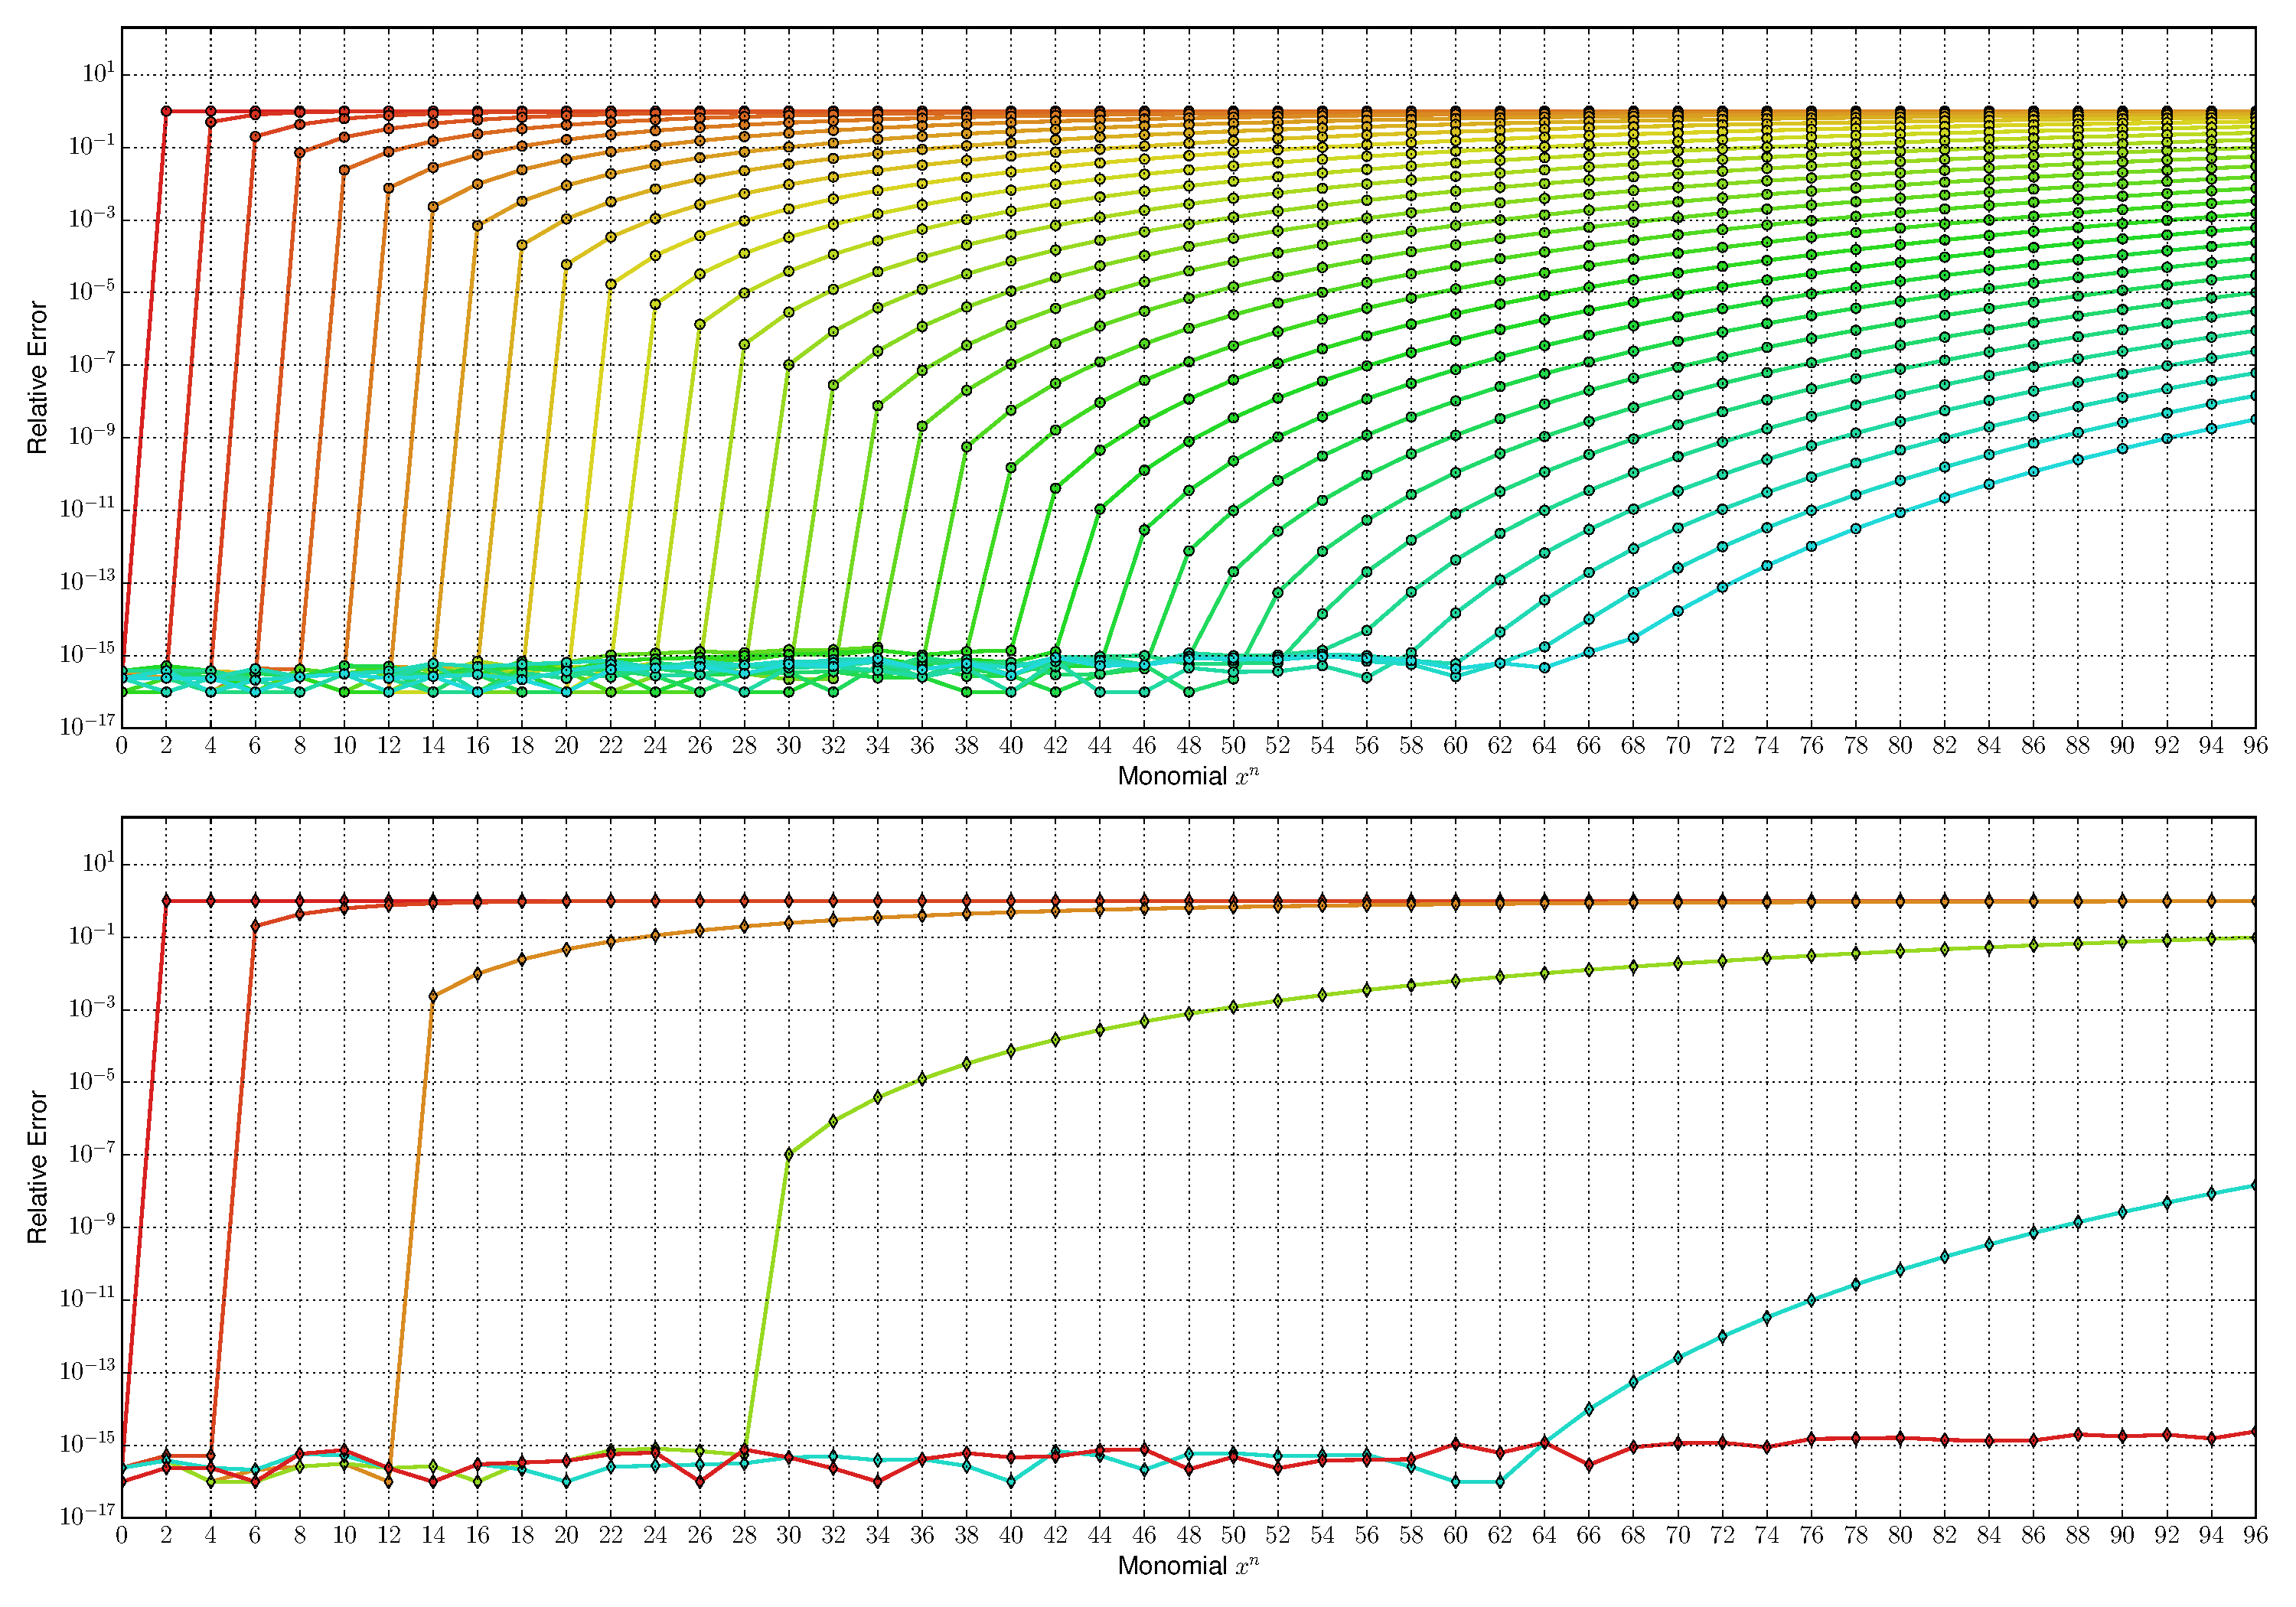
\includegraphics[width=\linewidth]{./img/monomial_errors_chebyshevu.pdf}
  \caption{Relative quadrature error for integration of single univariate monomials $x^n$ of increasing degree $n$.
  Each line represents a quadrature rule and the color indicates the number of nodes (colors wrap around once though).
  The upper plot shows Gauss-Chebyshev rules as reference while the lower one shows the Genz-Keister rules.
  The number of nodes for each of these rules is:
  $1$, $3$,  $7$, $15$, $31$,  $63$ and the orders according to \eqref{eq:gk_rul_order} are:
  $1$, $5$, $13$, $29$, $61$, $125$ which perfectly agrees with the figure.
  The error is in good agreement with the Gauss-Chebyshev rules which is of course
  expected because the rules are identical.}
  \label{fig:monomial_errors_chebyshevu}
\end{figure}

\begin{figure}[h]
  \centering
  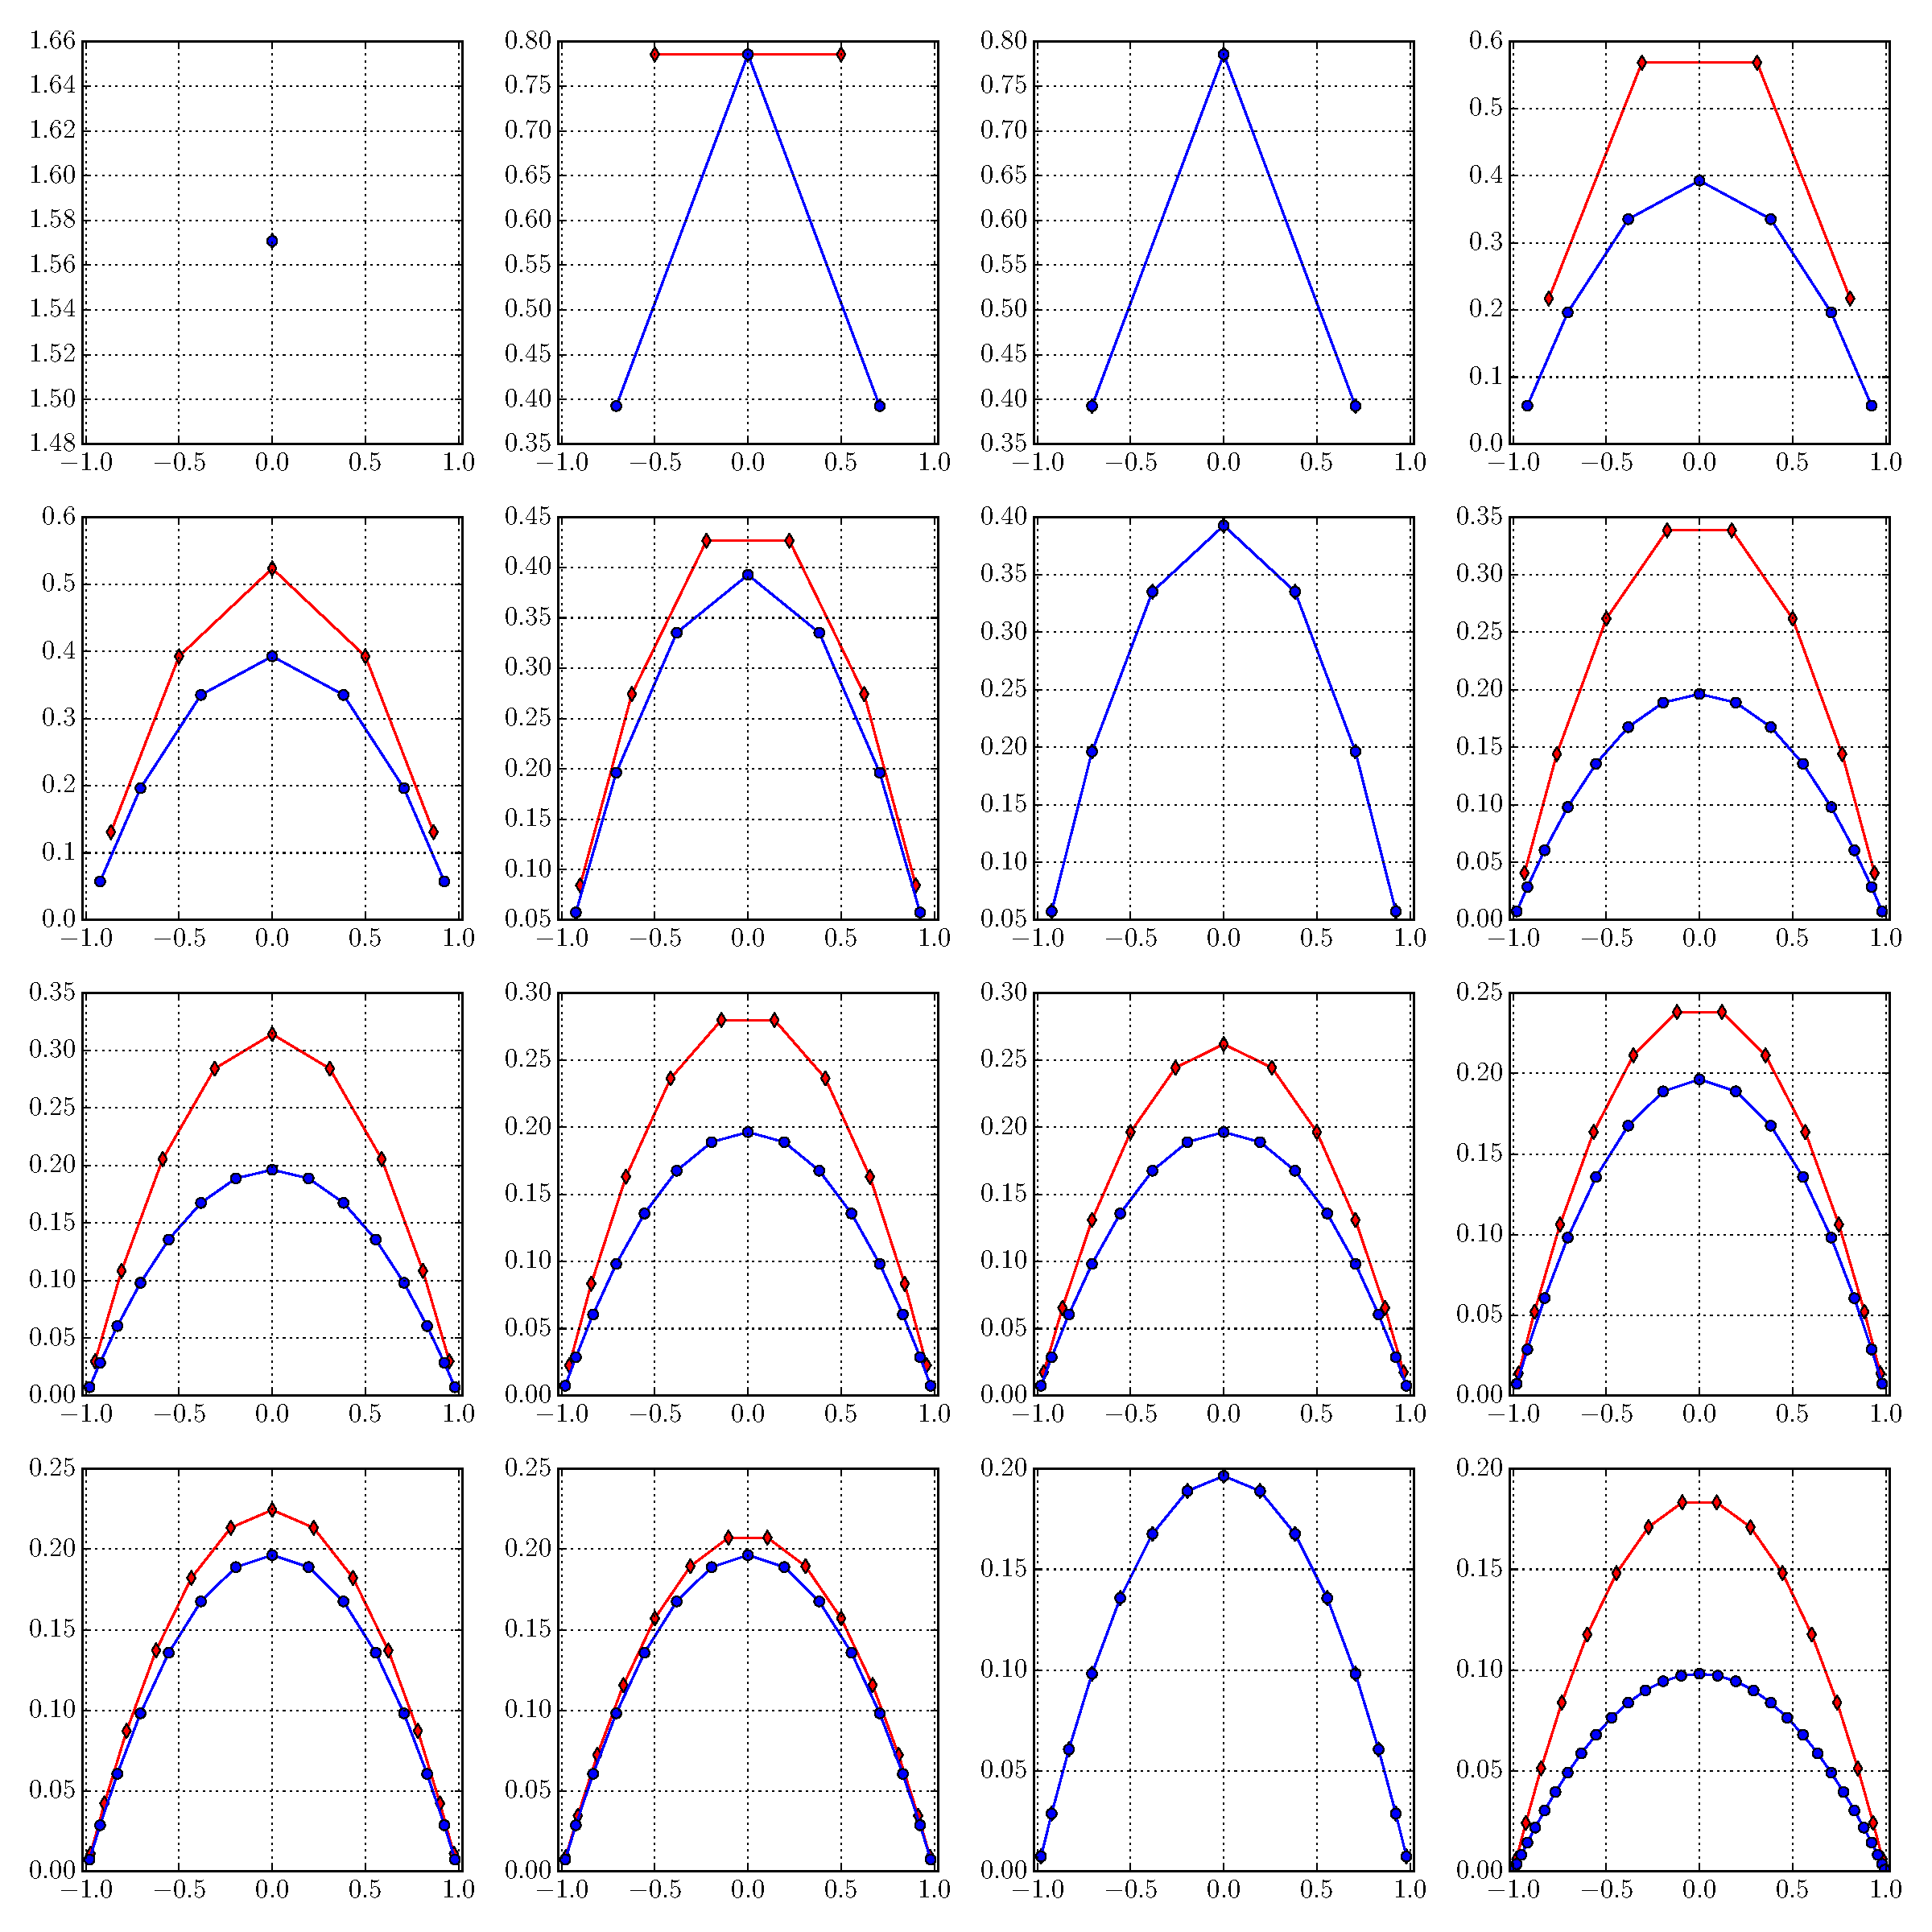
\includegraphics[width=\linewidth]{./img/gk_chebyshevu_nodes_1d.pdf}
  \caption{Gauss-Chebyshev (red) and Genz-Keister (blue) nodes versus
  corresponding weights. All $(2^i-1)$-point rules are identical.}
  \label{fig:gk_chebyshevu_nodes_1d}
\end{figure}

\begin{figure}[h]
  \centering
  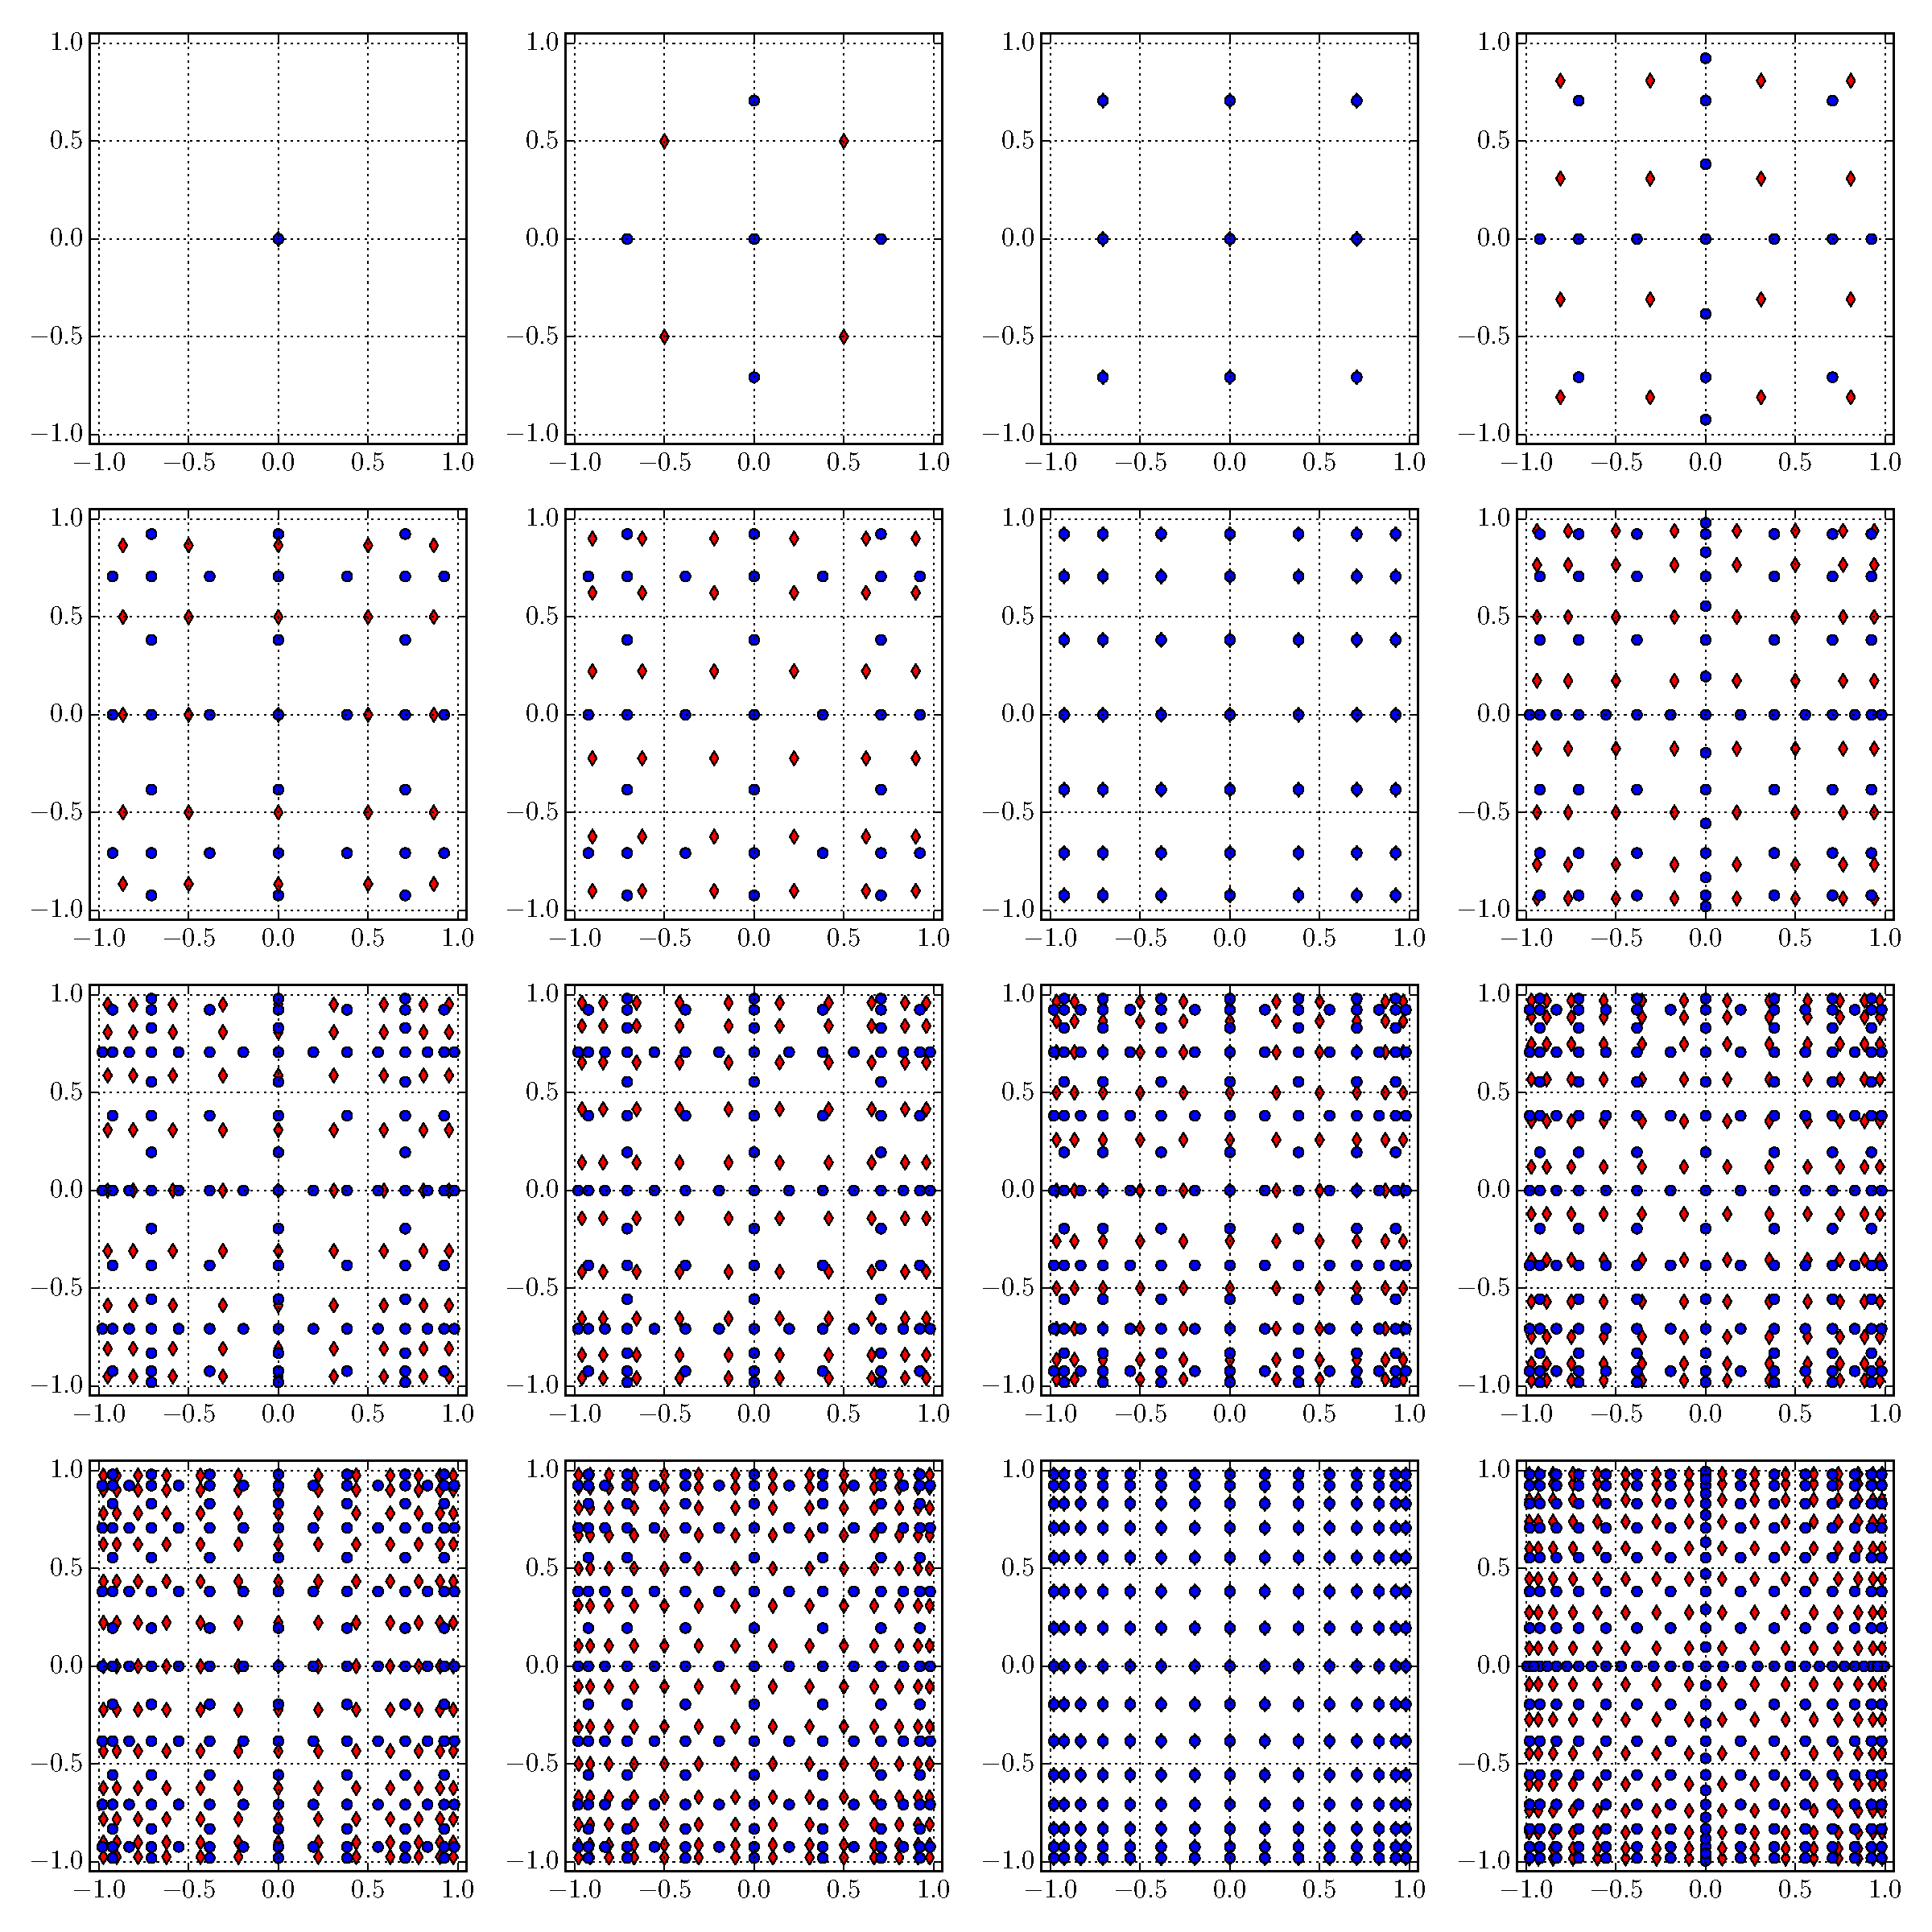
\includegraphics[width=\linewidth]{./img/gk_chebyshevu_nodes_2d.pdf}
  \caption{Gauss-Chebyshev (red) and Genz-Keister (blue) nodes for
  two-dimensional rules. The Gauss-Chebyshev points form a full tensor
  product.}
  \label{fig:gk_chebyshevu_nodes_2d}
\end{figure}

\begin{figure}
  \centering
  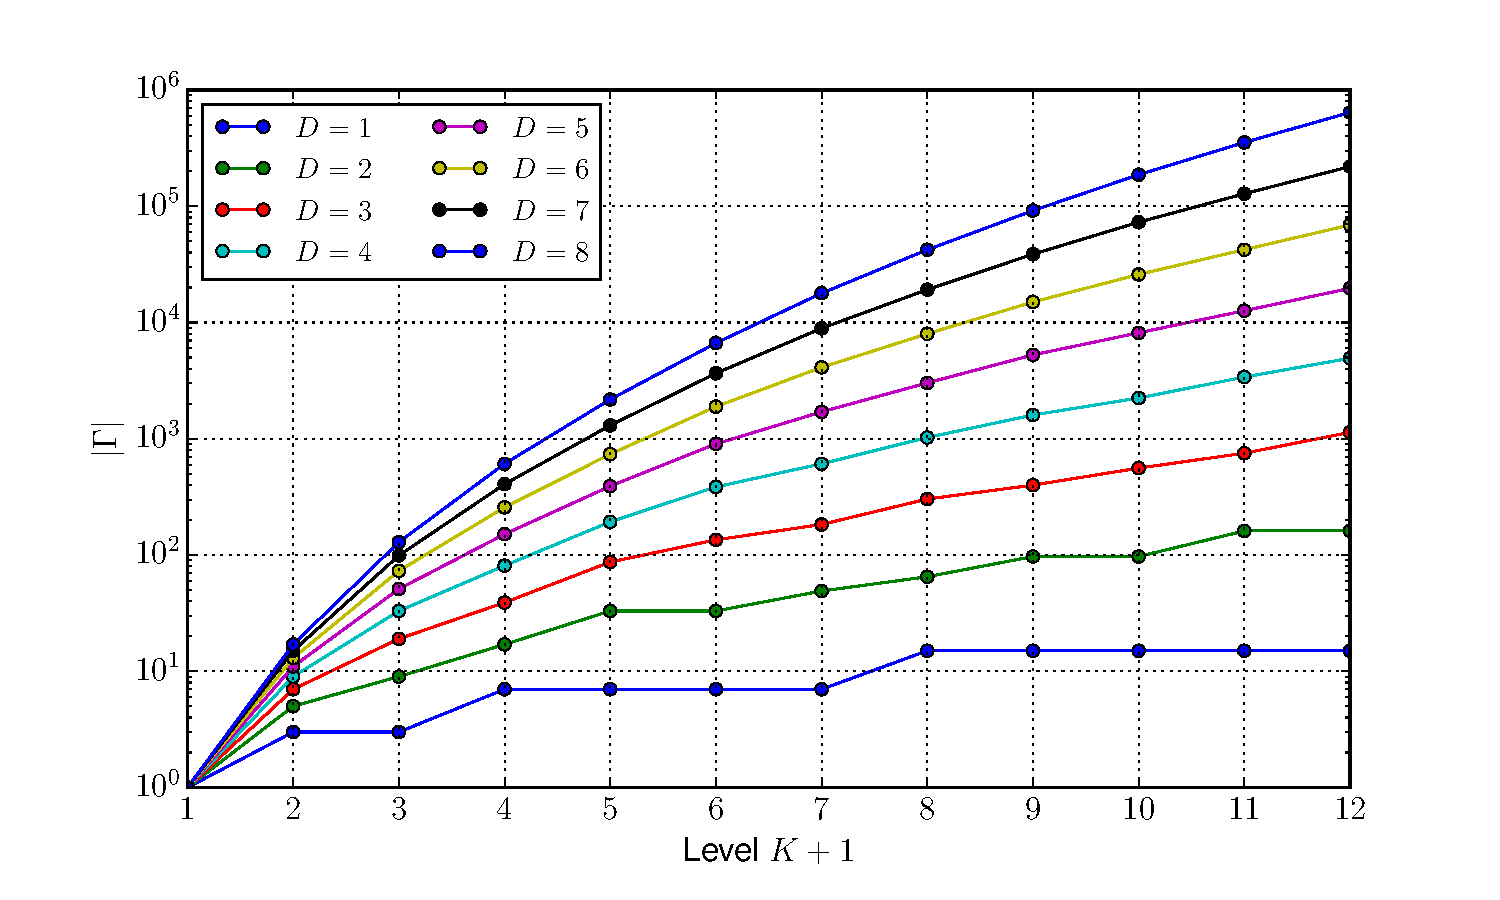
\includegraphics[width=\linewidth]{./img/number_nodes_levdim_chebyshevu.pdf}
  \caption{Number $|\Gamma|$ of Genz-Keister quadrature nodes for various levels $K$ and dimensions $D$.}
  \label{fig:number_nodes_levdim_chebyshevu}
\end{figure}

\begin{figure}[h]
  \centering
  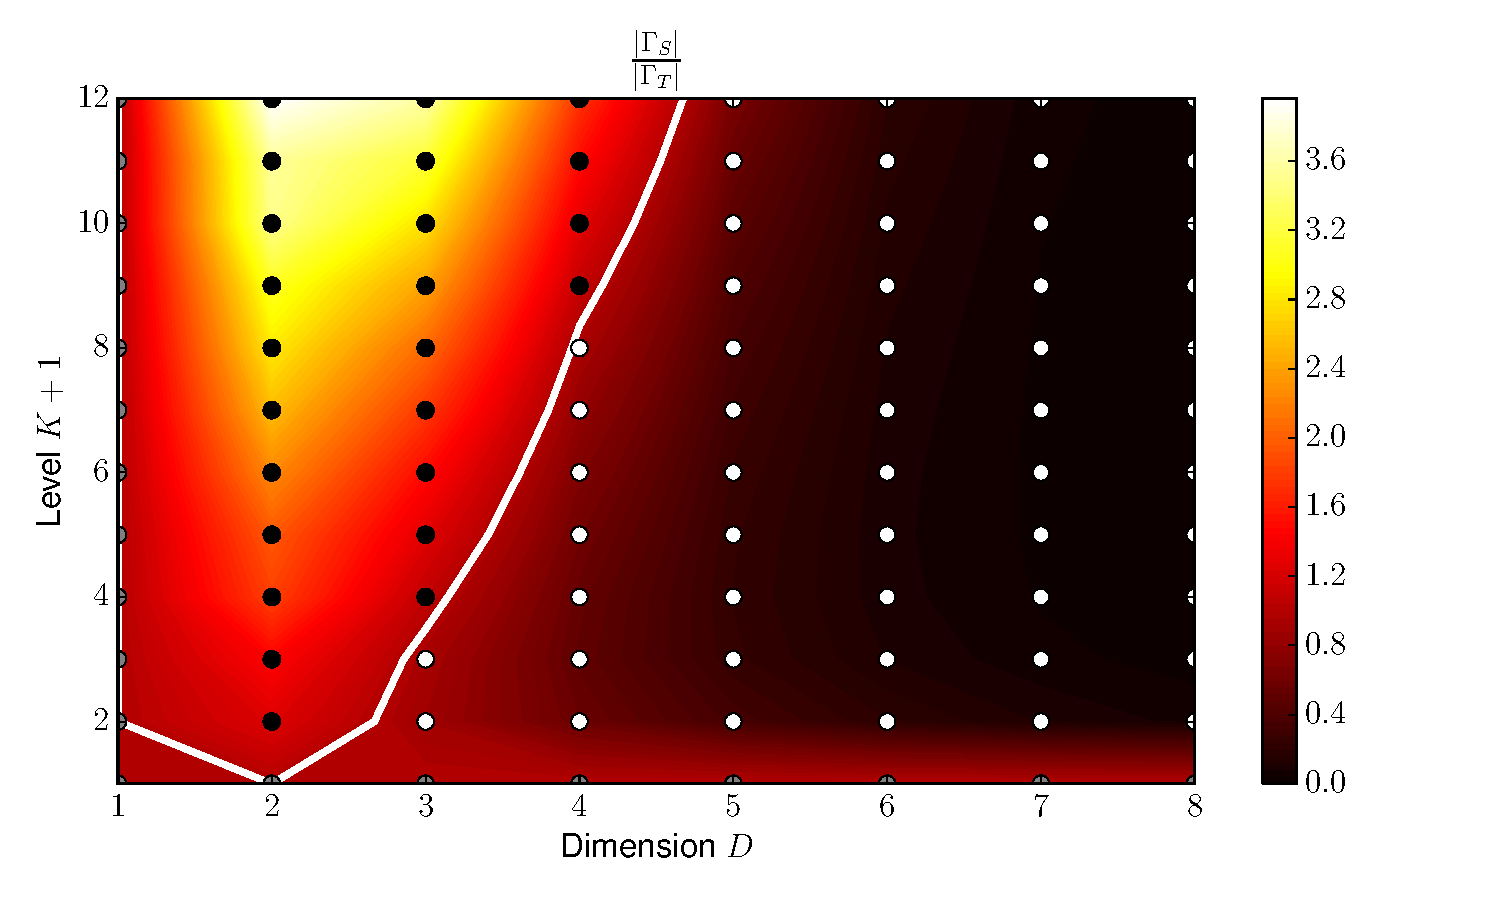
\includegraphics[width=0.8\linewidth]{./img/smol_chebyshevu_ratio.pdf}
  \caption{Ratio of the number of Gauss-Chebyshev quadrature points obtained
  via tensor product and classical Smolyak construction. White dots are $D,K$
  combinations where Genz-Keister is advantageous, while for black dots
  Genz-Keister is worse and for gray dots the ratio equals 1.
  Notice that although some of the Gauss rules are already nested, this has
  (as expected) almost no effect when applying the Smolyak construction.
  The only difference between this figure and its siblings is the point
  $D=4$ and $K=8$ which here is white instead of black. Also the boundary
  will reach $D=5$ a few levels later. However there is obviously still
  room for improvement.}
  \label{fig:smol_chebyshevu_ratio}
\end{figure}

\begin{figure}[h]
  \centering
  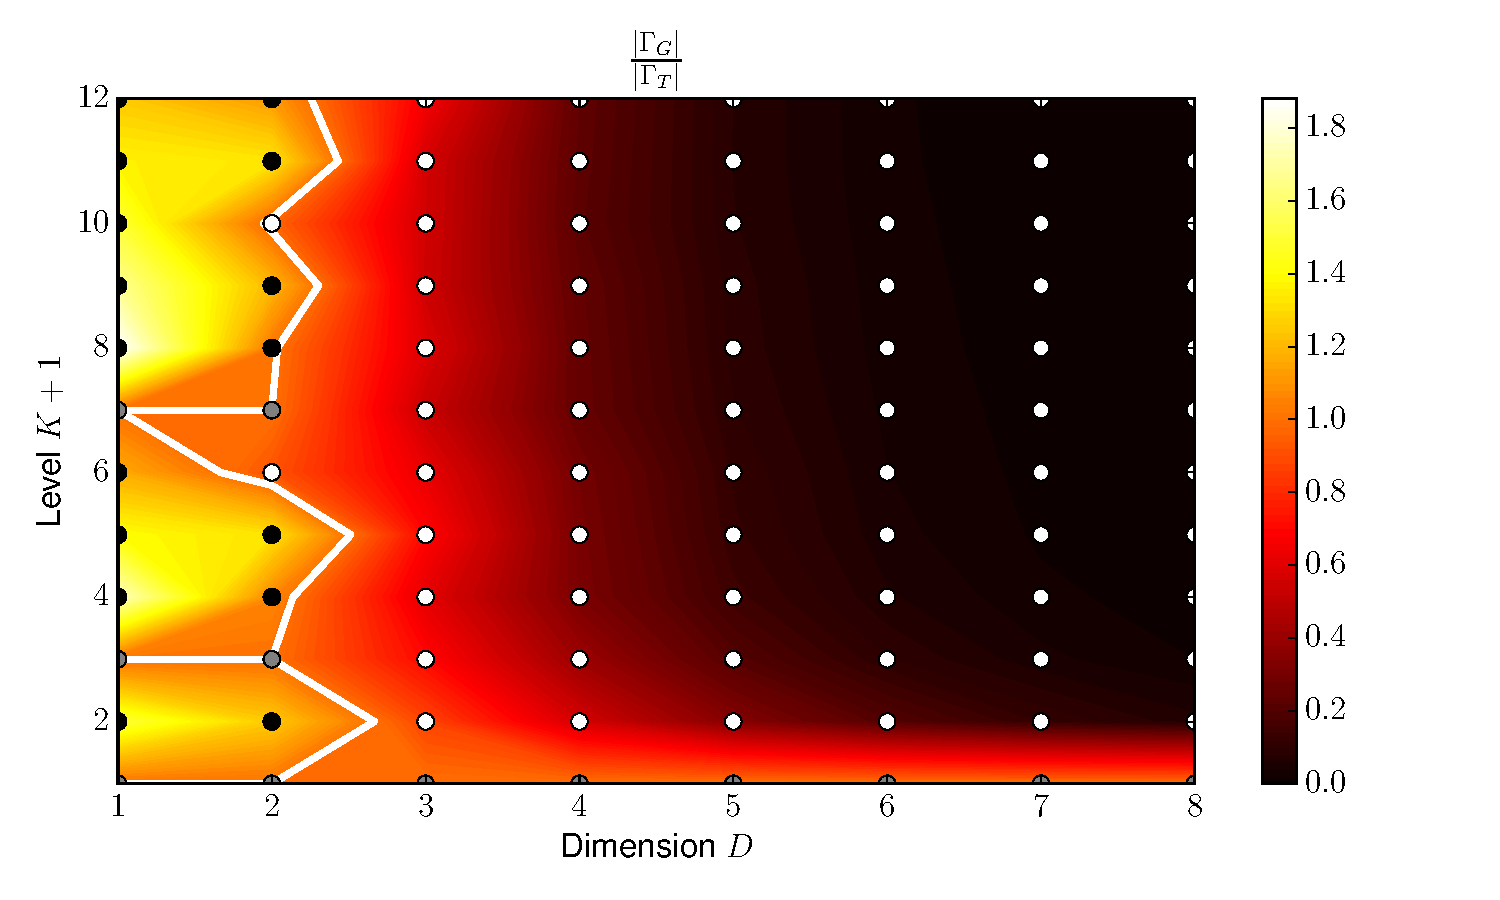
\includegraphics[width=0.8\linewidth]{./img/gk_chebyshevu_ratio.pdf}
  \caption{Ratio of the number of Genz-Keister and Gauss-Chebyshev tensor product
  points for dimensions $D$ up to 8 and Level $K \leq 12$. White dots are $D,K$
  combinations where Genz-Keister is advantageous, while for black dots
  Genz-Keister is worse and for gray dots the ratio equals 1.}
  \label{fig:gk_chebyshevu_ratio}
\end{figure}

\begin{figure}[h]
  \centering
  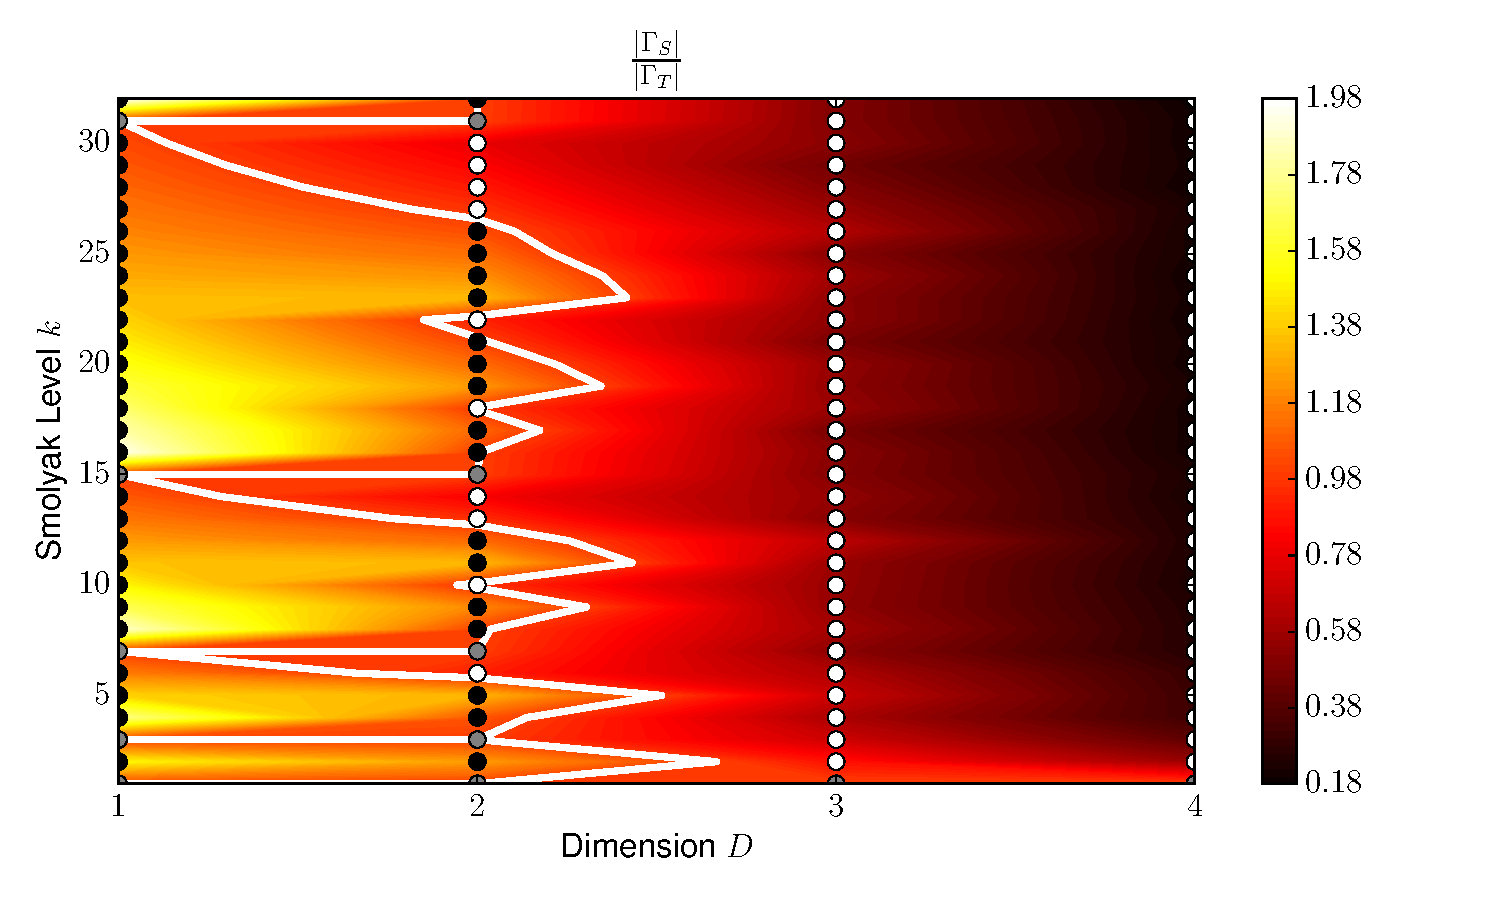
\includegraphics[width=0.8\linewidth]{./img/gk_chebyshevu_ratio_large.pdf}
  \caption{Ratio of the number of Genz-Keister and Gauss-Chebyshev tensor product
  points for dimensions 1 to 4 and Level $K \leq 32$. White dots are $D,K$
  combinations where Genz-Keister is advantageous, while for black dots
  Genz-Keister is worse and for gray dots the ratio equals 1.}
  \label{fig:gk_chebyshevu_ratio_large}
\end{figure}

For testing the quadrature rules in $D$ dimensions, the following integral
over multi-variate monomials with $\vec{n} \in \mathbb{N}_0^D$ is used:
\begin{equation} \label{eq:chebyshevu_exact_solution}
  \idotsint \limits_{\vec{x} \in [-1,1]^D} \prod_{d=1}^D x_d^{n_d} \sqrt{1-x_d^2} \di{\vec{x}}
  =
  \left(\frac{\sqrt{\pi}}{4}\right)^D
  \prod_{d=1}^D \left(1 + (-1)^{n_d}\right)
  \frac{\Gamma\left(\frac{n_d}{2}+\frac{1}{2}\right)}
       {\Gamma\left(\frac{n_d}{2}+2\right)}
\end{equation}
where we know the exact solution in closed form.

\begin{subfigures}
  \label{fig:monomial_errors_chebyshevu_multivariate}
  \begin{figure}\centering
    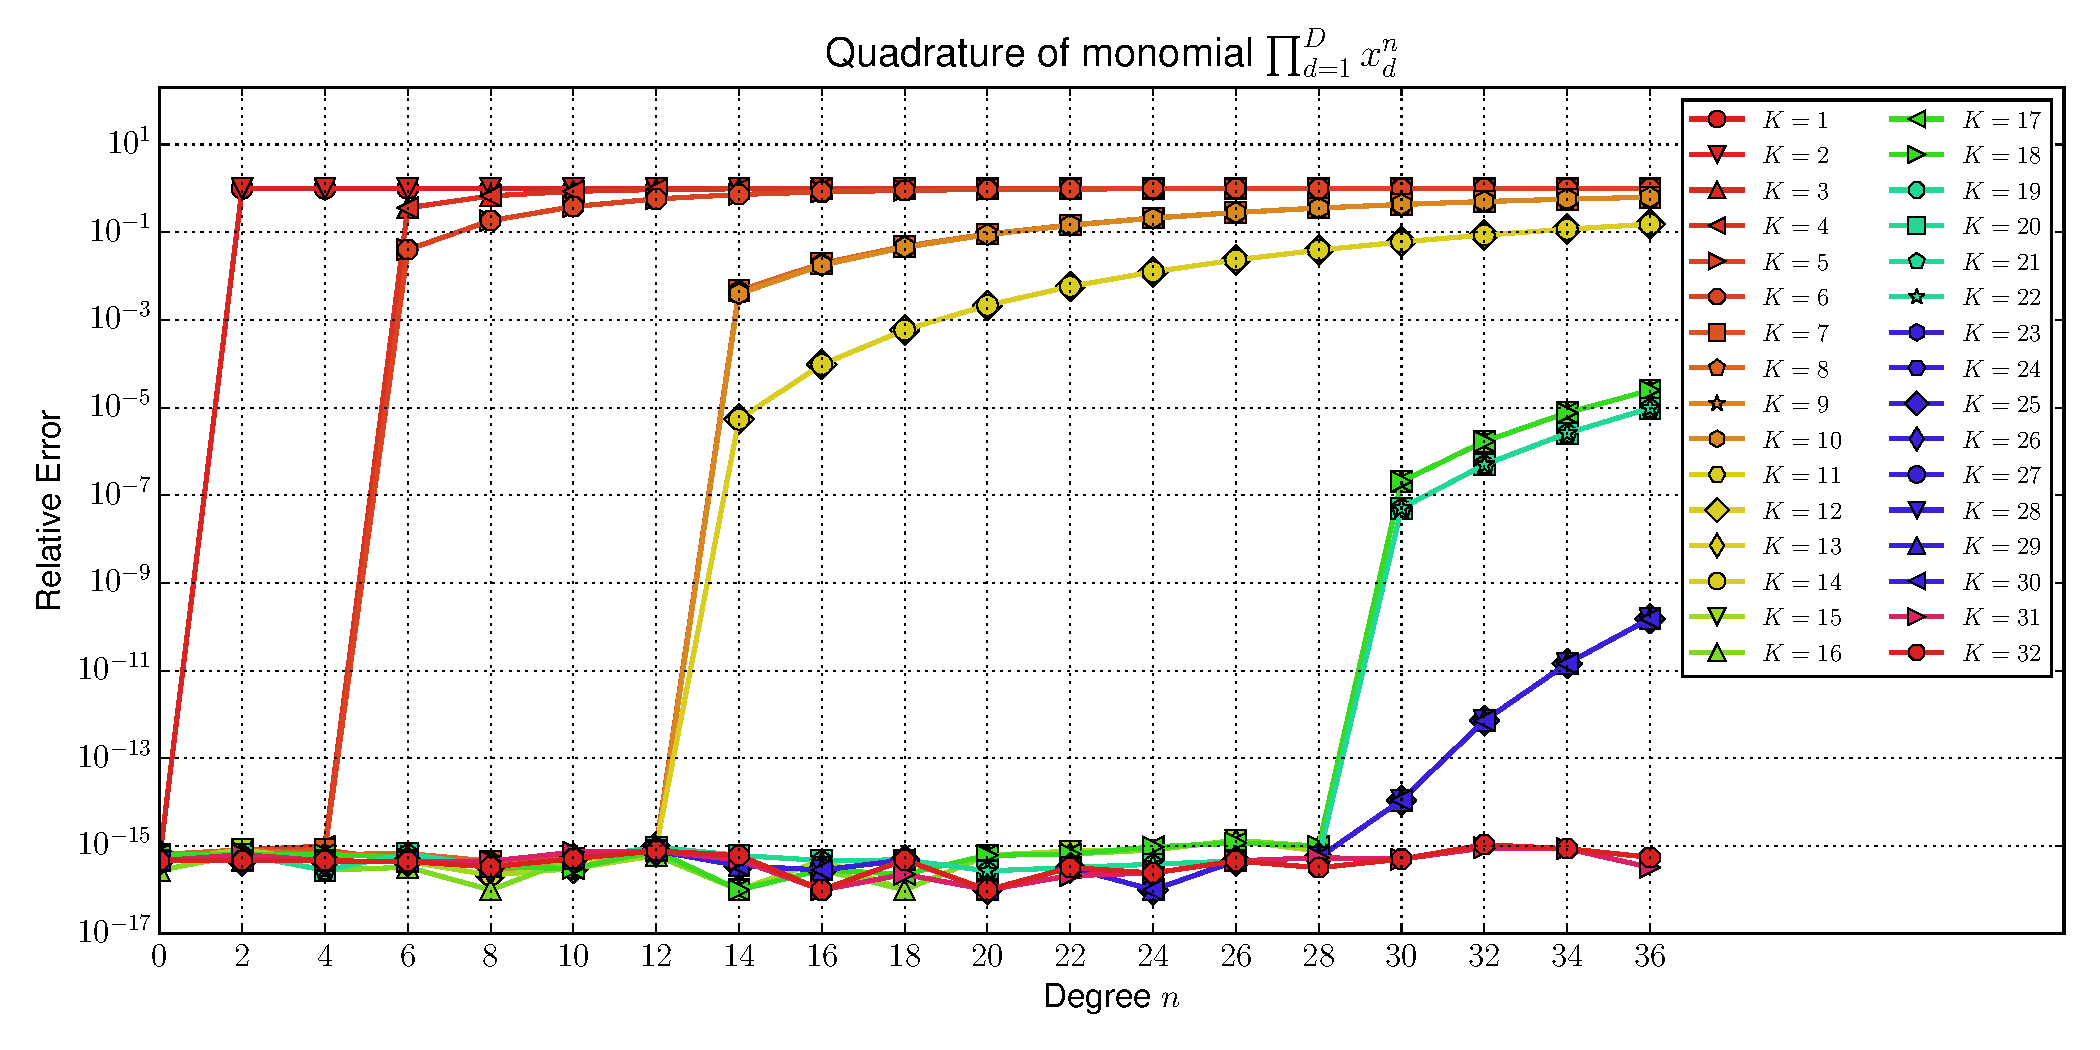
\includegraphics[width=\linewidth]{./img/monomial_errors_chebyshevu_multivariate_dimension_2.pdf}
    \caption{Relative errors for the integral \eqref{eq:chebyshevu_exact_solution}
    in $D=2$ dimensions. All variables $x_d$ share the same exponent $n$.}
    \label{fig:monomial_errors_chebyshevu_multivariate_dimension_2}
  \end{figure}
  \begin{figure}\centering
    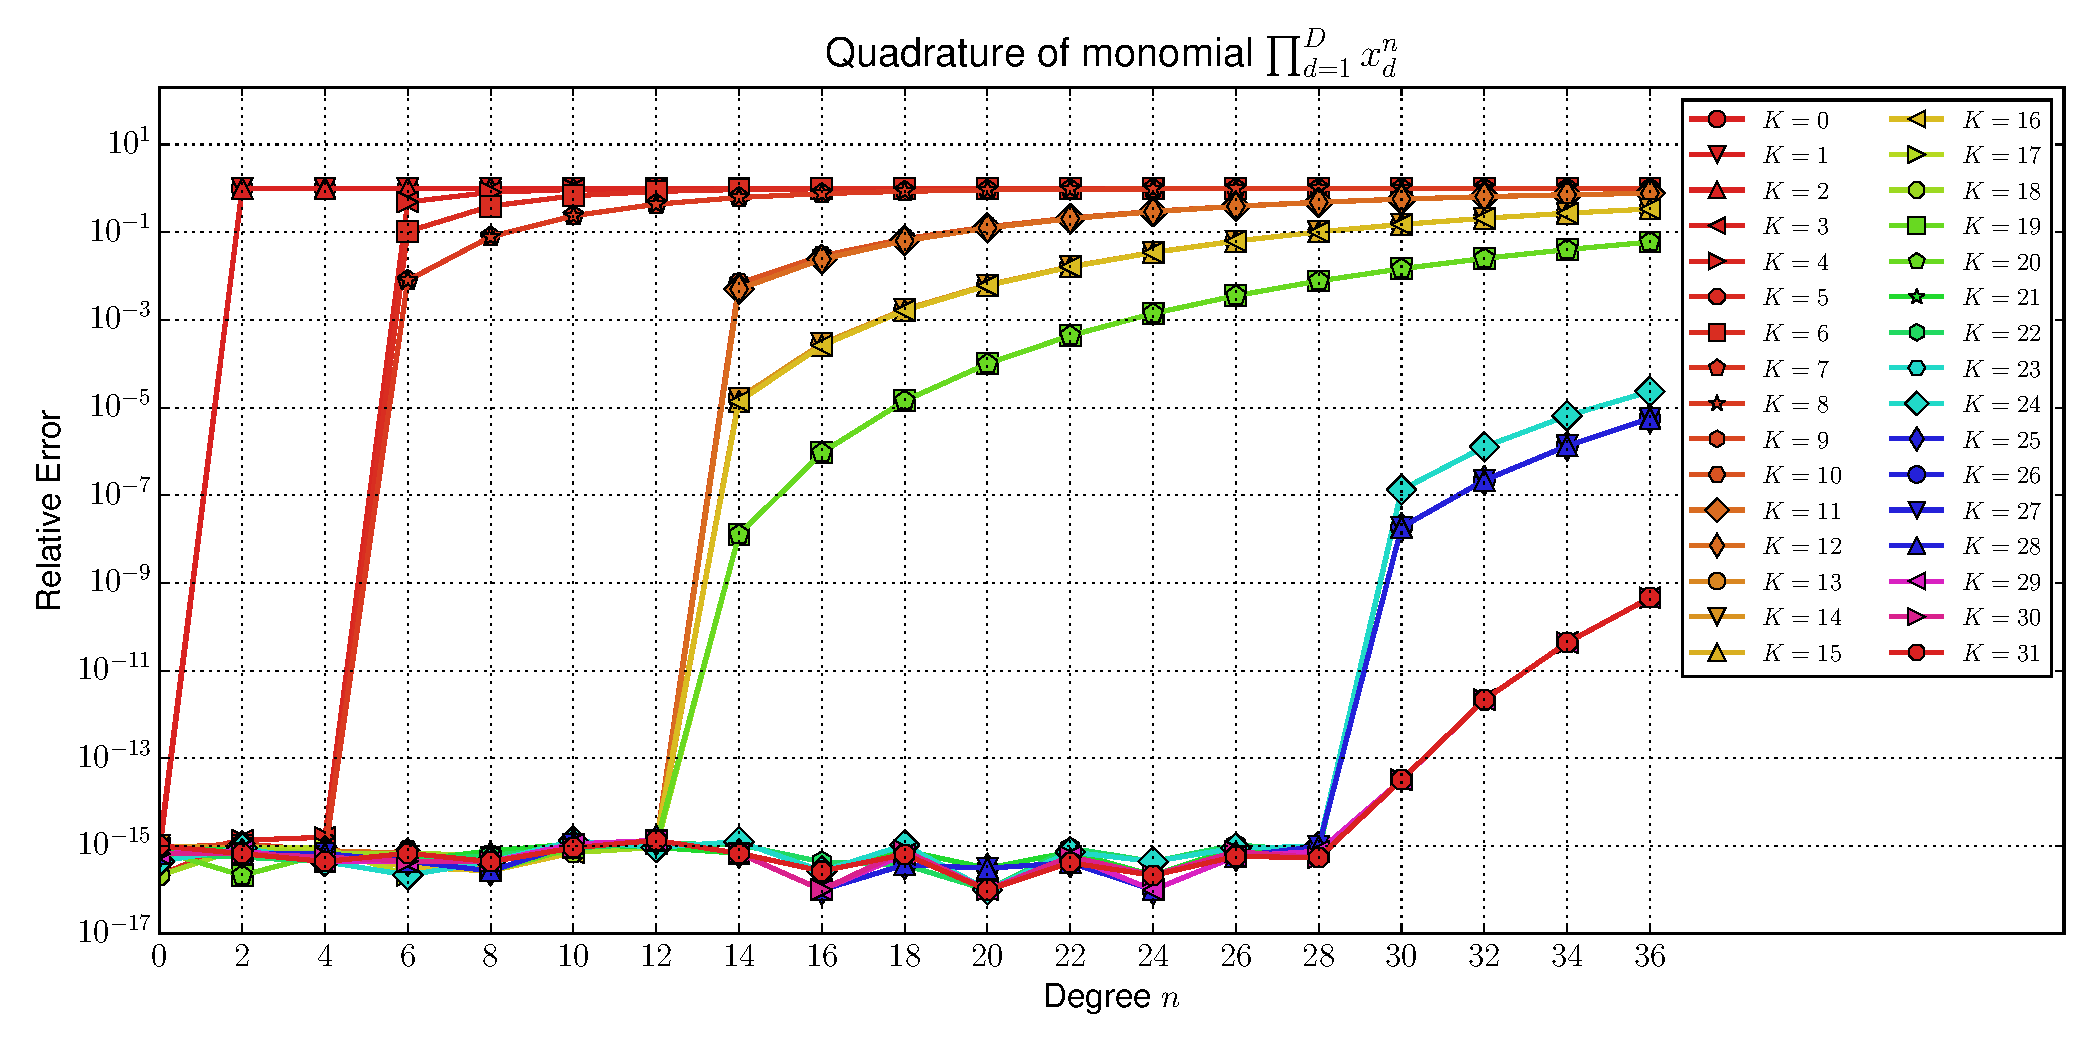
\includegraphics[width=\linewidth]{./img/monomial_errors_chebyshevu_multivariate_dimension_3.pdf}
    \caption{Relative errors for the integral \eqref{eq:chebyshevu_exact_solution}
    in $D=3$ dimensions. All variables $x_d$ share the same exponent $n$.}
    \label{fig:monomial_errors_chebyshevu_multivariate_dimension_3}
  \end{figure}
  \begin{figure}\centering
    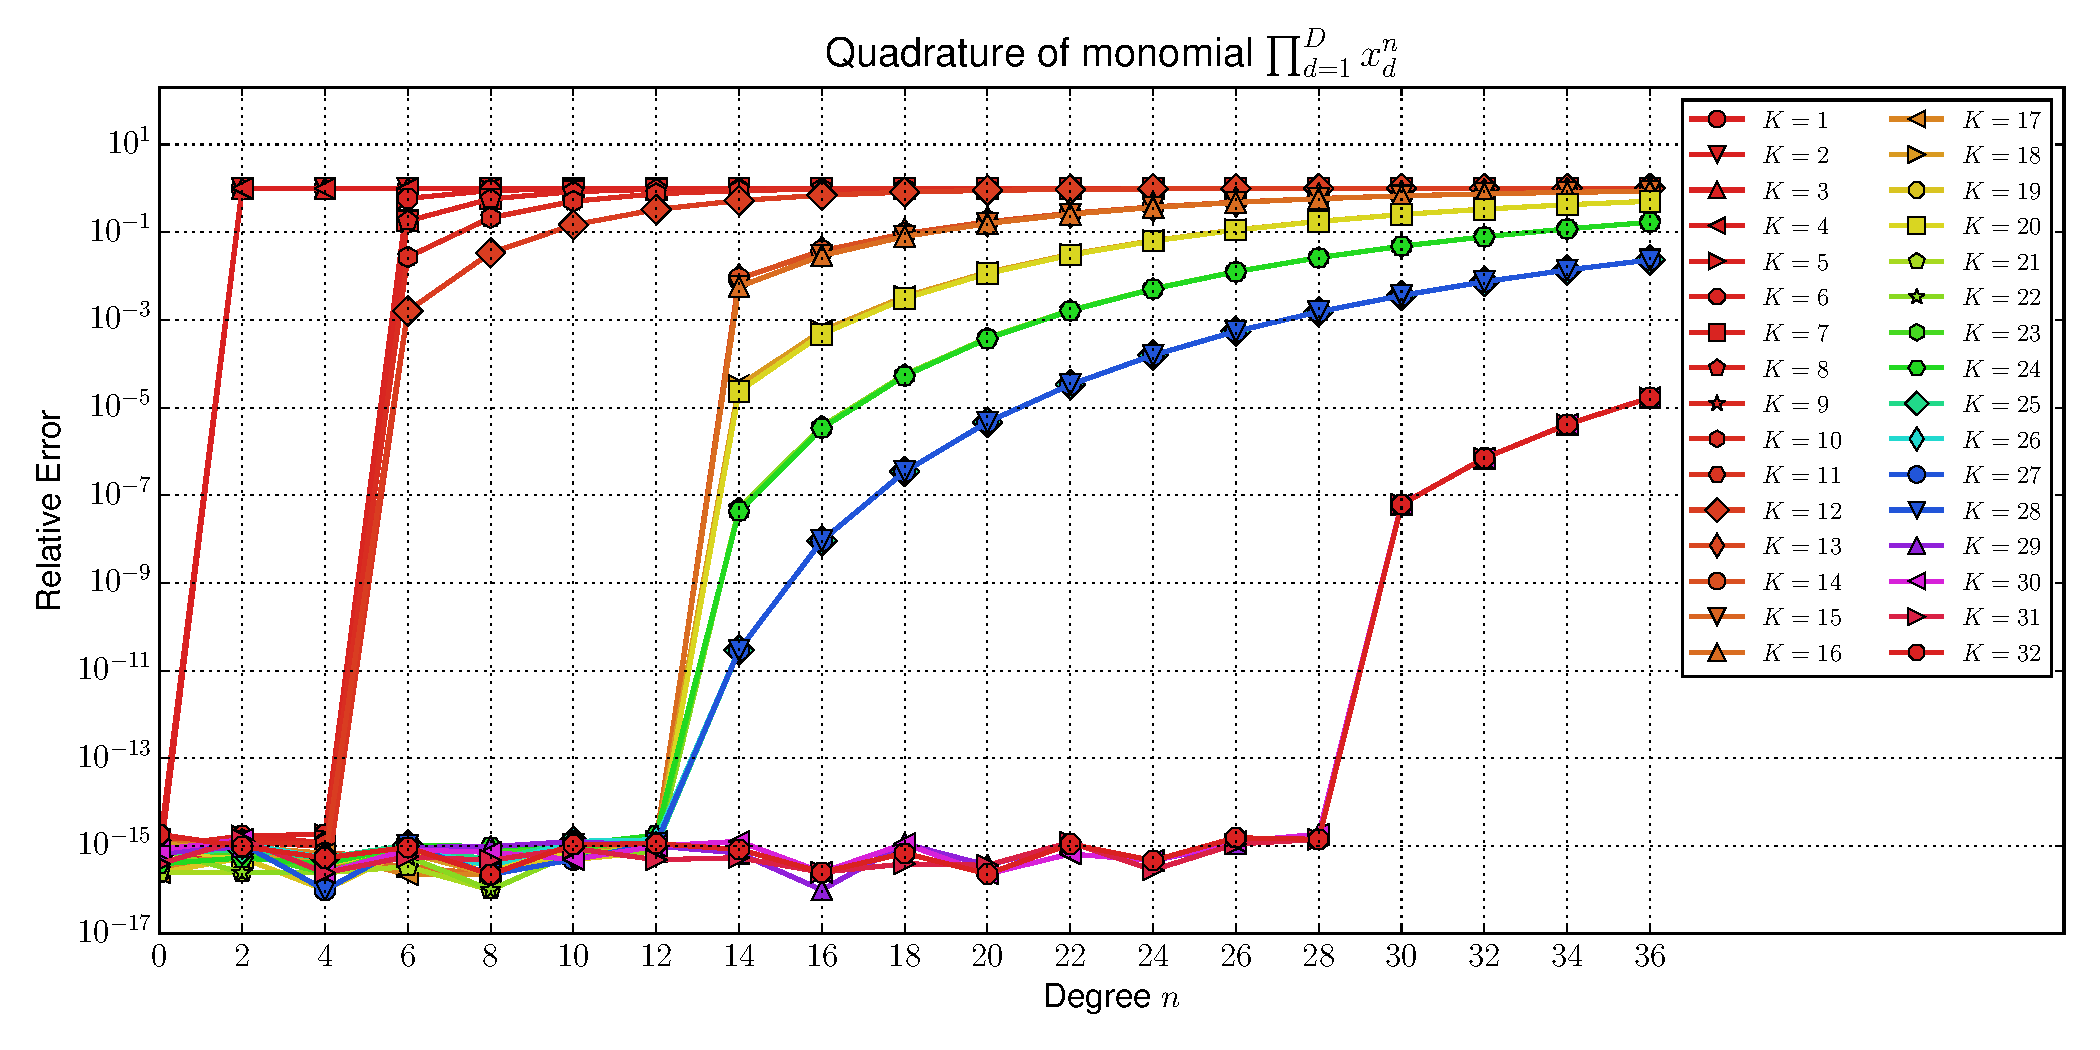
\includegraphics[width=\linewidth]{./img/monomial_errors_chebyshevu_multivariate_dimension_4.pdf}
    \caption{Relative errors for the integral \eqref{eq:chebyshevu_exact_solution}
    in $D=4$ dimensions. All variables $x_d$ share the same exponent $n$.}
    \label{fig:monomial_errors_chebyshevu_multivariate_dimension_4}
  \end{figure}
  \begin{figure}\centering
    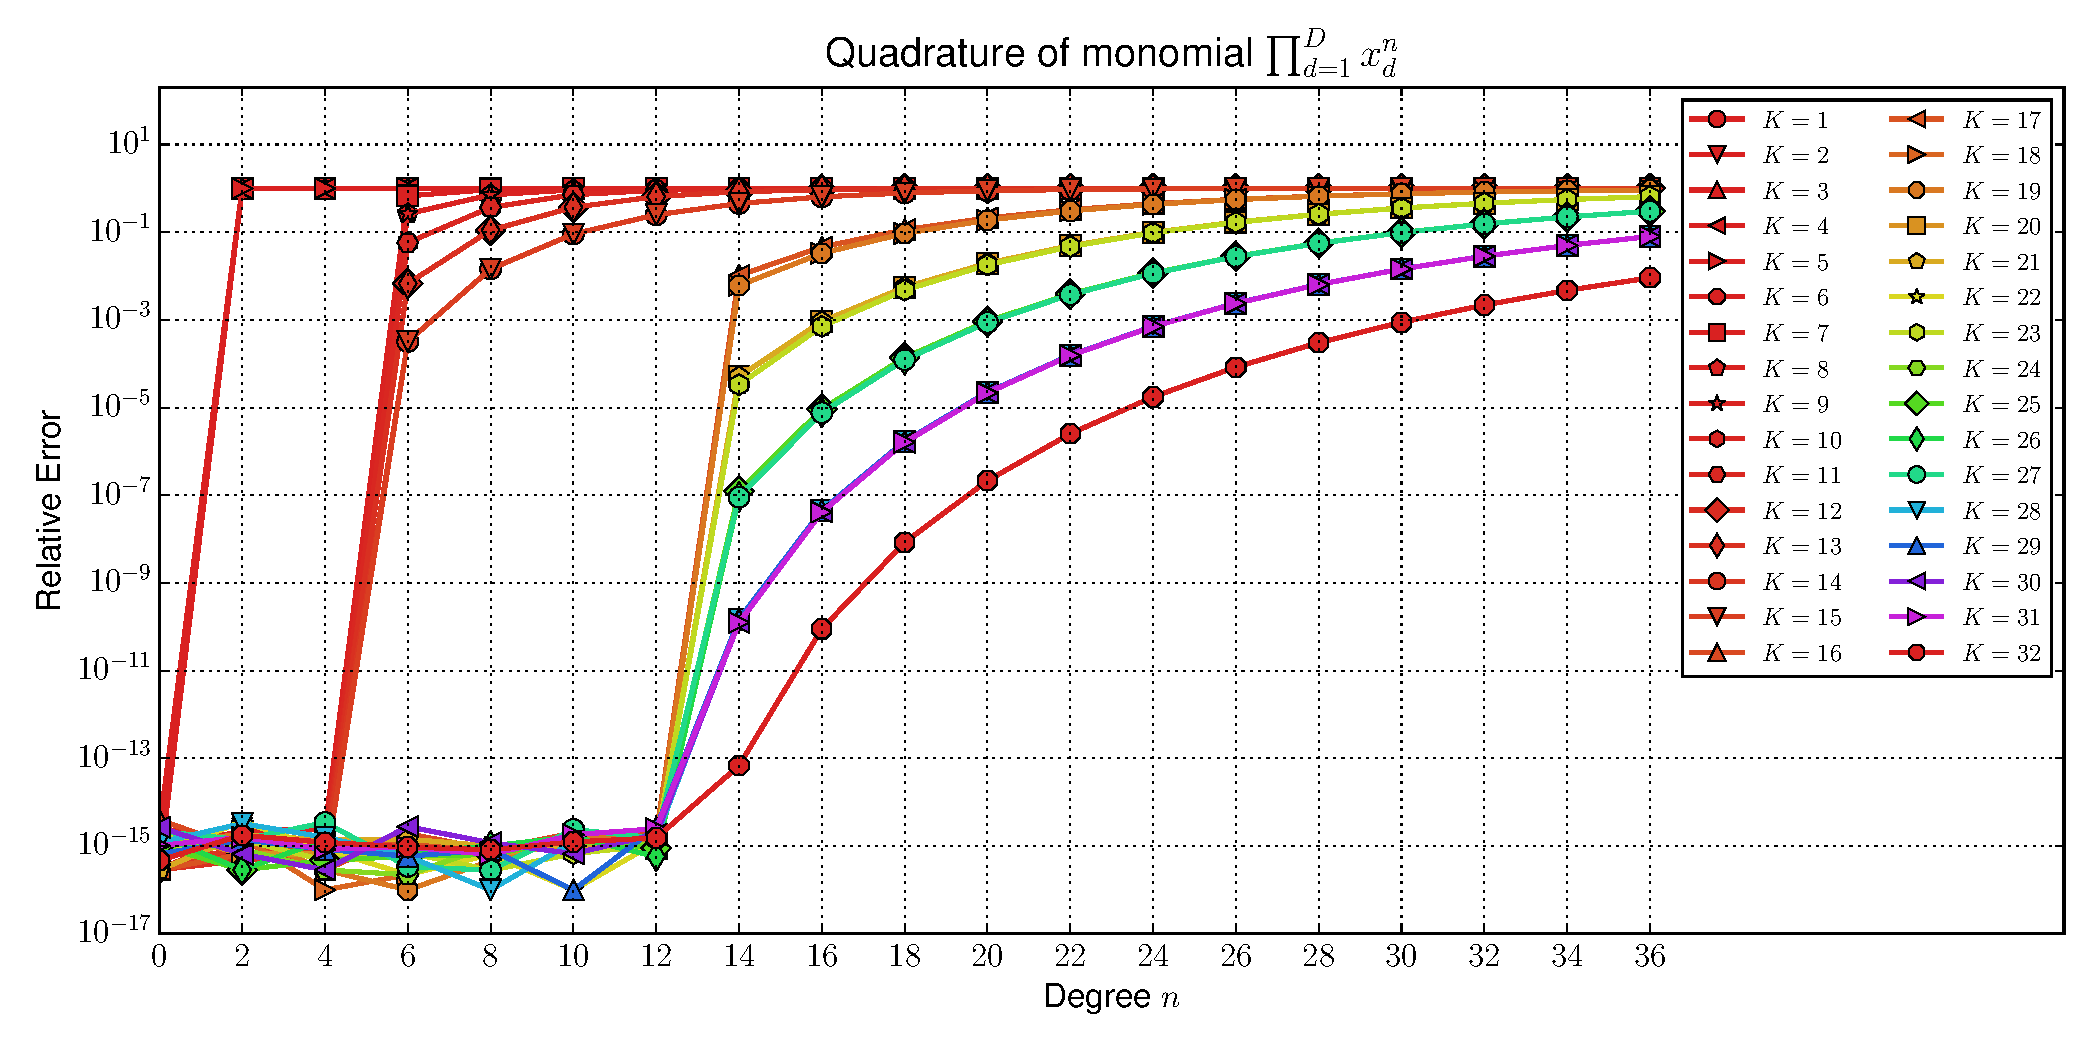
\includegraphics[width=\linewidth]{./img/monomial_errors_chebyshevu_multivariate_dimension_5.pdf}
    \caption{Relative errors for the integral \eqref{eq:chebyshevu_exact_solution}
    in $D=5$ dimensions. All variables $x_d$ share the same exponent $n$.}
    \label{fig:monomial_errors_chebyshevu_multivariate_dimension_5}
  \end{figure}
  \begin{figure}\centering
    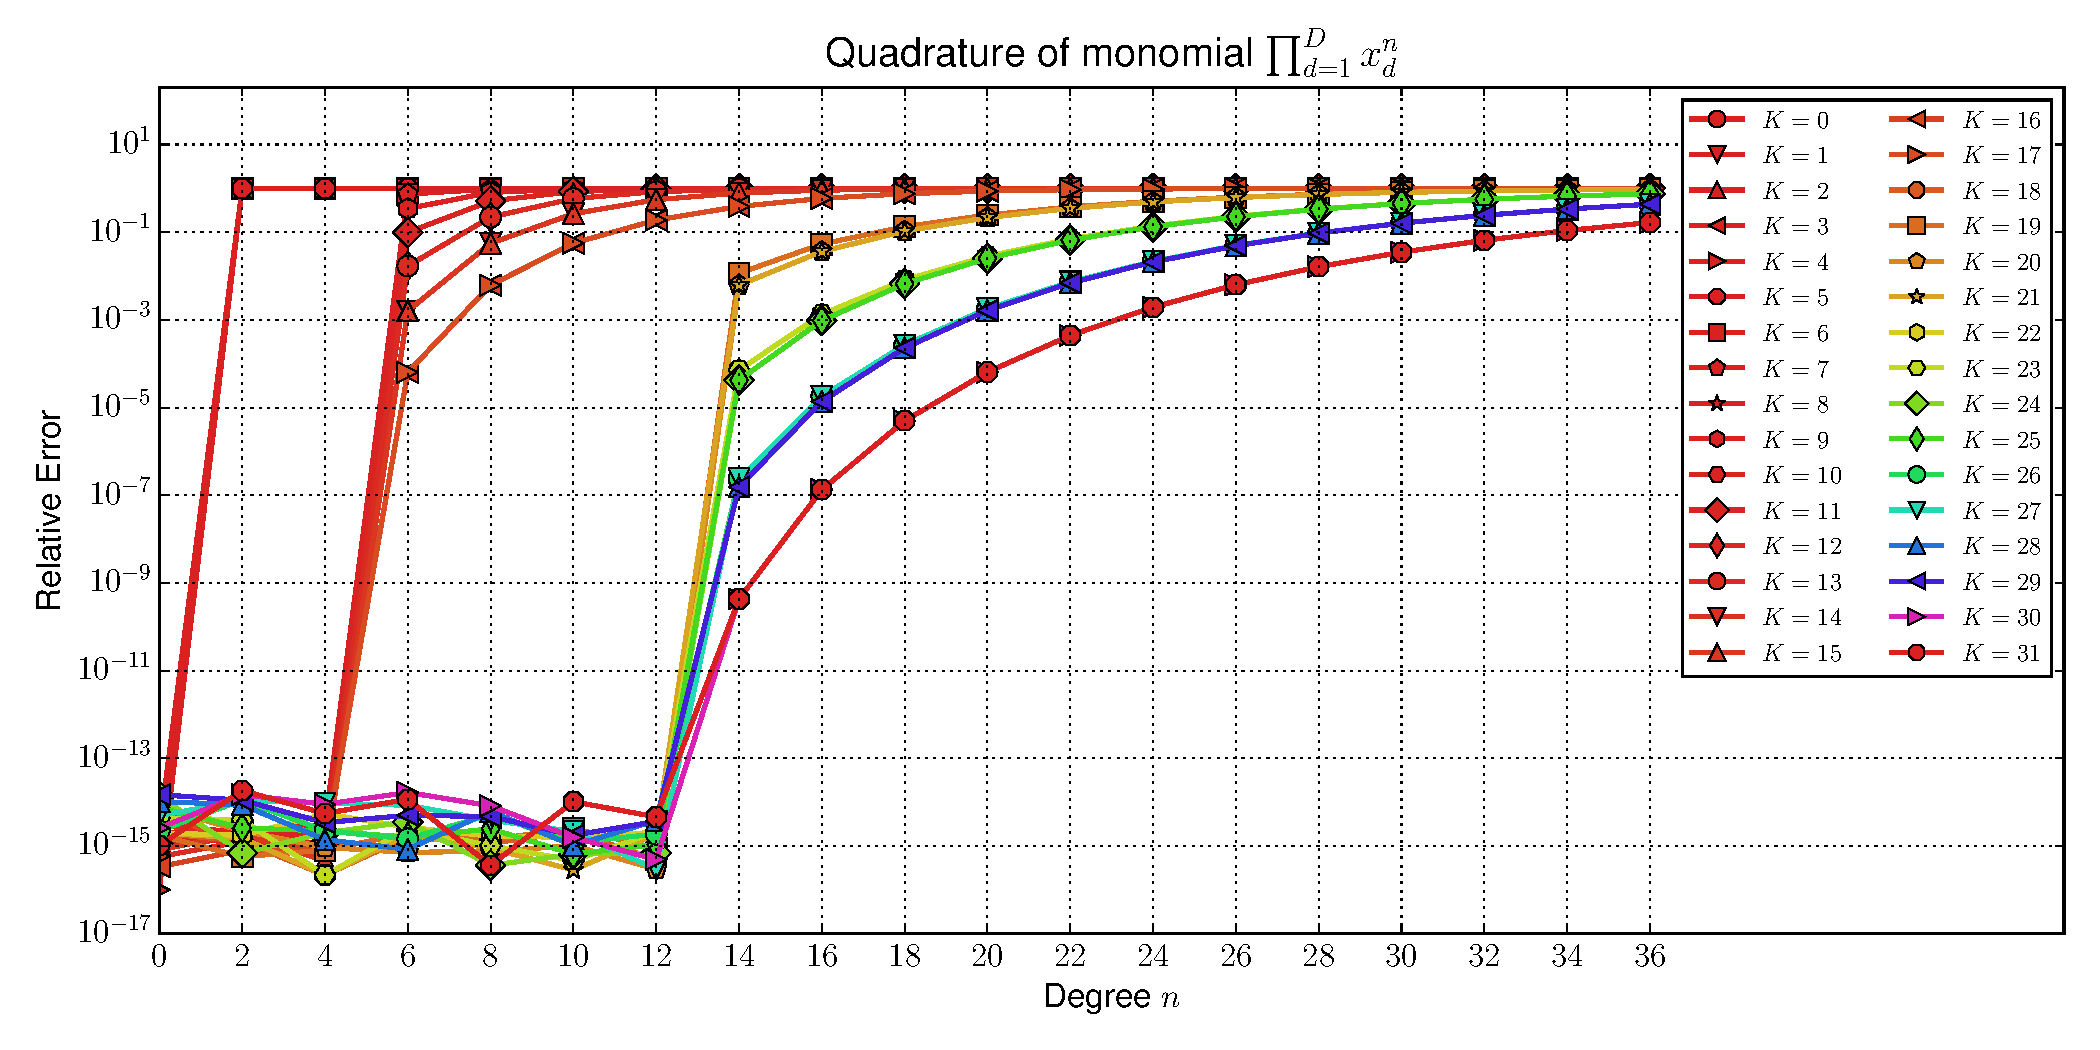
\includegraphics[width=\linewidth]{./img/monomial_errors_chebyshevu_multivariate_dimension_6.pdf}
    \caption{Relative errors for the integral \eqref{eq:chebyshevu_exact_solution}
    in $D=6$ dimensions. All variables $x_d$ share the same exponent $n$.}
    \label{fig:monomial_errors_chebyshevu_multivariate_dimension_6}
  \end{figure}
\end{subfigures}

\FloatBarrier
\subsection{Hermite Quadrature}

Figure \ref{fig:smol_hermitephy_ratio} shows the comparison of a full tensor
and a Smolyak construction based on the usual Gauss-Hermite points. Obviously the region
where Smolyak is disadvantageous extends to higher dimensions and this at even relatively
low levels. This is clearly an issue and should give some motivation for studying the
Genz-Keister constructions.
For Hermite polynomials $H_n$ Kronrod extensions are rare, especially extensions
having a high nesting degree. One of the best such extensions found so far is
$\mathcal{K} = (1, 2, 6, 10, 16, 68)$ with the $z$ sequence:
\begin{equation*}
  \vec{z} = (0, 0, 1, 0, 0, 3, 2, 1, 0, 0, 5, 4, 3, 2, 1, 0, 0, 0, 8, 7,
             6, 5, 4, 3, 2, 1, 0, 0, 0, 0, 0, 0, \ldots)
             %0 0 0 0 0 0 0 0 0 0 0 0 0 0 0 0 0 0 0 0 0)
\end{equation*}
Using this extension we get the one-dimensional quadrature nodes and weights shown
in Figure \ref{fig:gk_hermitephy_nodes_1d}.
Figure \ref{fig:gk_hermitephy_nodes_2d} shows the sparse
node distribution in the plane for two-dimensional quadrature rules.

\begin{figure}[h]
  \centering
  \includegraphics[width=\linewidth]{./img/gk_hermitephy_nodes_cmp.pdf}
  \caption{Comparison of Gauss-Hermite nodes (right) and nested Genz-Keister nodes (left)
  based on the $\mathcal{K} = (1, 2, 6, 10, 16, 68)$ Kronrod extension. The points are
  nicely nested and well suited for sparse grids.}
  \label{fig:gk_hermitephy_nodes_cmp}
\end{figure}

\begin{figure}
  \centering
  \includegraphics[width=\linewidth]{./img/number_nodes_hermitephy.pdf}
  \caption{Number of nodes for the one-dimensional Gauss-Hermite and Genz-Keister quadrature
  rules of order $n$ or level $K$ respectively.}
  \label{fig:number_nodes_hermitephy}
\end{figure}

\begin{figure}
  \centering
  \includegraphics[width=\linewidth]{./img/monomial_errors_hermitephy.pdf}
  \caption{Relative quadrature error for integration of single univariate monomials $x^n$ of increasing degree $n$.
  Each line represents a quadrature rule and the color indicates the number of nodes (colors wrap around once though).
  The upper plot shows Gauss-Hermite rules as reference while the lower one shows the Genz-Keister rules.
  The number of nodes for each of these rules is:
  $1$, $3$, $7$,  $9$, $17$, $19$, $31$, $33$, $35$
  and the orders according to \eqref{eq:gk_rul_order} are:
  $1$, $5$, $7$, $15$, $17$, $29$, $31$, $33$, $51$
  which perfectly agrees with the figure. Given that none of the higher order rules agree with any Gauss-Hermite rule,
  the stability and error behavior is excellent. On the other hand, the rule with $35$ points integrates monomials
  correctly only up to $x^{51}$ with $51 = 2 \cdot 25 + 1$ instead of up to $n = 2 \cdot 35 - 1 = 69$.}
  \label{fig:conv_monom_hermite}
\end{figure}

By comparing to Figure \ref{fig:conv_monom_hermite} we can confirm that the rules with $K < 18$ are stable.
The rule obtained with $K=17$ has $35$ nodes and is of order $51$. In the range $18 < K \leq 25$ we get no
new rules but rather the same nodes and weights as with $K = 17$. Rules with even higher $K > 25$ were found
to be highly unstable.

\begin{figure}[h]
  \centering
  \includegraphics[width=\linewidth]{./img/gk_hermitephy_nodes_1d.pdf}
  \caption{Gauss-Hermite (red) and Genz-Keister (blue) nodes versus
  corresponding weights. The 1- and 3-point rules are identical.}
  \label{fig:gk_hermitephy_nodes_1d}
\end{figure}

\begin{figure}[h]
  \centering
  \includegraphics[width=\linewidth]{./img/gk_hermitephy_nodes_2d.pdf}
  \caption{Gauss-Hermite (red) and Genz-Keister (blue) nodes for
  two-dimensional rules. The Gauss-Hermite points form a full tensor
  product.}
  \label{fig:gk_hermitephy_nodes_2d}
\end{figure}

\begin{figure}
  \centering
  \includegraphics[width=\linewidth]{./img/number_nodes_levdim_hermitephy.pdf}
  \caption{Number $|\Gamma|$ of Genz-Keister quadrature nodes for various levels $K$ and dimensions $D$.}
  \label{fig:number_nodes_levdim_hermitephy}
\end{figure}

\begin{figure}[h]
  \centering
  \includegraphics[width=0.8\linewidth]{./img/smol_hermitephy_ratio.pdf}
  \caption{Ratio of the number of Gauss-Hermite quadrature points obtained
  via tensor product and classical Smolyak construction. White dots are $D,K$
  combinations where Genz-Keister is advantageous, while for black dots
  Genz-Keister is worse and for gray dots the ratio equals 1.}
  \label{fig:smol_hermitephy_ratio}
\end{figure}

Notice that for $D < 3$, using the Genz-Keister construction results
in more quadrature points than the full tensor product Ansatz. This
can be read off from Figures \ref{fig:gk_hermitephy_ratio}
and \ref{fig:gk_hermitephy_ratio_large}.

\begin{figure}[h]
  \centering
  \includegraphics[width=0.8\linewidth]{./img/gk_hermitephy_ratio.pdf}
  \caption{Ratio of the number of Genz-Keister and Gauss-Hermite tensor product
  points for dimensions $D$ up to 8 and Level $K \leq 12$. White dots are $D,K$
  combinations where Genz-Keister is advantageous, while for black dots
  Genz-Keister is worse and for gray dots the ratio equals 1.}
  \label{fig:gk_hermitephy_ratio}
\end{figure}

\begin{figure}[h]
  \centering
  \includegraphics[width=0.8\linewidth]{./img/gk_hermitephy_ratio_large.pdf}
  \caption{Ratio of the number of Genz-Keister and Gauss-Hermite tensor product
  points for dimensions 1 to 4 and Level $K \leq 32$. White dots are $D,K$
  combinations where Genz-Keister is advantageous, while for black dots
  Genz-Keister is worse and for gray dots the ratio equals 1. Even if not visible here,
  the white boundary will go more to the right and reach dimension $D = 3$ at level $K = 51$.}
  \label{fig:gk_hermitephy_ratio_large}
\end{figure}

\begin{figure}
  \centering
  \includegraphics[width=\linewidth]{./img/monomial_errors_hermitephy_high.pdf}
  \caption{Relative quadrature error for integration of single univariate monomials $x^n$ of increasing degree $n$.
  Each line represents a quadrature rule and the color indicates the number of nodes (colors wrap around once though).
  The number of nodes for each of these rules is:
  $53$, $55$, $57$, $59$, $61$, $63$, $65$, $67$, $69$, $71$, $73$, $75$,  $77$,
  $79$, $81$, $83$, $85$, $87$, $89$, $91$, $93$, $95$, $97$, $99$, $101$, $103$.
  The rules for $K > 25$ become soon highly unstable. A notable exception is the
  last rule with $K = 51$ having $103$ nodes which shows good behavior and
  is of order $103$. This is obviously extremely inefficient for practical
  use.}
  \label{fig:conv_monom_hermite_high}
\end{figure}

\begin{figure}[h]
  \centering
  \includegraphics[width=\linewidth]{./img/monomial_errors_hermitephy_2D.pdf}
  \caption{Quadrature of the bivariate monomials $x^m y^n$ for $0 \leq n, m \leq 50$.
  Each pair $(m,n)$ is color-coded by the lowest level $K$ rule that correctly
  integrates the monomial with a relative error not larger than $10^{-13}$.}
  \label{fig:monomial_errors_hermitephy_2D}
\end{figure}

For testing the quadrature rules in $D$ dimensions, the following integral
over multi-variate monomials with $\vec{n} \in \mathbb{N}_0^D$ is used:
\begin{equation} \label{eq:hermitephy_exact_solution}
  \idotsint \limits_{\vec{x} \in \mathbb{R}^D} \prod_{d=1}^D x_d^{n_d} \exp\left(-x_d^2\right) \di{\vec{x}}
  =
  \frac{1}{2^D} \prod_{d=1}^D \left(1 + (-1)^{n_d}\right) \Gamma\left(\frac{n_d + 1}{2}\right)
\end{equation}
where we know the exact solution in closed form.

\begin{subfigures}
  \label{fig:monomial_errors_hermitephy_multivariate}
  \begin{figure}\centering
    \includegraphics[width=\linewidth]{./img/monomial_errors_hermitephy_multivariate_dimension_2.pdf}
    \caption{Relative errors for the integral \eqref{eq:hermitephy_exact_solution}
    in $D=2$ dimensions. All variables $x_d$ share the same exponent $n$.}
    \label{fig:monomial_errors_hermitephy_multivariate_dimension_2}
  \end{figure}
  \begin{figure}\centering
    \includegraphics[width=\linewidth]{./img/monomial_errors_hermitephy_multivariate_dimension_3.pdf}
    \caption{Relative errors for the integral \eqref{eq:hermitephy_exact_solution}
    in $D=3$ dimensions. All variables $x_d$ share the same exponent $n$.}
    \label{fig:monomial_errors_hermitephy_multivariate_dimension_3}
  \end{figure}
  \begin{figure}\centering
    \includegraphics[width=\linewidth]{./img/monomial_errors_hermitephy_multivariate_dimension_4.pdf}
    \caption{Relative errors for the integral \eqref{eq:hermitephy_exact_solution}
    in $D=4$ dimensions. All variables $x_d$ share the same exponent $n$.}
    \label{fig:monomial_errors_hermitephy_multivariate_dimension_4}
  \end{figure}
  \begin{figure}\centering
    \includegraphics[width=\linewidth]{./img/monomial_errors_hermitephy_multivariate_dimension_5.pdf}
    \caption{Relative errors for the integral \eqref{eq:hermitephy_exact_solution}
    in $D=5$ dimensions. All variables $x_d$ share the same exponent $n$.}
    \label{fig:monomial_errors_hermitephy_multivariate_dimension_5}
  \end{figure}
  \begin{figure}\centering
    \includegraphics[width=\linewidth]{./img/monomial_errors_hermitephy_multivariate_dimension_6.pdf}
    \caption{Relative errors for the integral \eqref{eq:hermitephy_exact_solution}
    in $D=6$ dimensions. All variables $x_d$ share the same exponent $n$.}
    \label{fig:monomial_errors_hermitephy_multivariate_dimension_6}
  \end{figure}
\end{subfigures}


\FloatBarrier
\section{Software}

The complete software used for this project can be downloaded at:

\begin{center}
  \url{https://github.com/raoulbq/kes.git}
\end{center}

and is released as free software under the GNU General Public License.


\FloatBarrier
\section{Future work}

A question is whether it would be computationally more efficient to compute
everything with arbitrary precision floating point ball arithmetic. By doing that
it might be possible to better handle the exponential growth of coefficients.
On the other hand, computing roots and solving for the weights seems to be
the most expensive part already.

By having efficient root isolation and counting algorithms in \texttt{flint} we would
not have to compute all roots of $E_p$ numerically to high precision just for answering
the question if some of them are complex hence marking the whole extension invalid
\footnote{This solution is also not fully satisfying since we can only
decide that a complex root is really complex but not if a candidate is for sure real.}.

Finally, this work is based on empirical studies on the outcome of algorithmic searches.
It would be desirable to have a rigorous mathematical foundation for the claims made.

Some of the techniques presented here could theoretically be generalized to Gegenbauer
polynomials $C_n^{(\alpha)}(x)$ and ultimately Jacobi polynomials $P_n^{(\alpha,\beta)}(x)$.
The parametric nature of these polynomials makes the implementation more complex. Also,
results will depend on the explicit values of these parameters $\alpha$ and $\beta$.

Similar techniques are actually applied in practical computations, for example
in the simulation of the Schr\"odinger equation \cite{tucker}.


\begin{appendix}
\section{Computed Generators}

The tables in this section contain the generator sets $\Lambda$ for all default
rules examined in the last sections. The generators are ordered in the above-mentioned
alternating order.

\begin{table}
  \centering
  \begin{tabular}{|l|ll|}
  \hline
  {}             & Generator                 & Error \\
  \hline
  $\lambda_{0}$  & $0$                       &  $\pm 0$ \\
  $\lambda_{1}$  & $0.77459666924148337704$  &  $\pm 8.9398 \cdot 10^{-128}$ \\
  $\lambda_{2}$  & $0.96049126870802028342$  &  $\pm 2.9519 \cdot 10^{-127}$ \\
  $\lambda_{3}$  & $0.434243749346802558$    &  $\pm 1.9264 \cdot 10^{-127}$ \\
  $\lambda_{4}$  & $0.99383196321275502221$  &  $\pm 1.2033 \cdot 10^{-125}$ \\
  $\lambda_{5}$  & $0.22338668642896688163$  &  $\pm 2.9048 \cdot 10^{-127}$ \\
  $\lambda_{6}$  & $0.88845923287225699889$  &  $\pm 1.6417 \cdot 10^{-125}$ \\
  $\lambda_{7}$  & $0.62110294673722640294$  &  $\pm 3.1186 \cdot 10^{-126}$ \\
  $\lambda_{8}$  & $0.99909812496766759766$  &  $\pm 4.2615 \cdot 10^{-122}$ \\
  $\lambda_{9}$  & $0.11248894313318662575$  &  $\pm 2.0256 \cdot 10^{-127}$ \\
  $\lambda_{10}$ & $0.98153114955374010687$  &  $\pm 6.0247 \cdot 10^{-122}$ \\
  $\lambda_{11}$ & $0.33113539325797683309$  &  $\pm 5.1636 \cdot 10^{-126}$ \\
  $\lambda_{12}$ & $0.92965485742974005667$  &  $\pm 2.6398 \cdot 10^{-122}$ \\
  $\lambda_{13}$ & $0.53131974364437562397$  &  $\pm 1.0295 \cdot 10^{-124}$ \\
  $\lambda_{14}$ & $0.8367259381688687355$   &  $\pm 7.0227 \cdot 10^{-123}$ \\
  $\lambda_{15}$ & $0.70249620649152707861$  &  $\pm 9.7952 \cdot 10^{-124}$ \\
  $\lambda_{16}$ & $0.99987288812035761194$  &  $\pm 9.0618 \cdot 10^{-115}$ \\
  $\lambda_{17}$ & $0.056344313046592789972$ &  $\pm 2.4195 \cdot 10^{-127}$ \\
  $\lambda_{18}$ & $0.99720625937222195908$  &  $\pm 1.446 \cdot 10^{-114}$ \\
  $\lambda_{19}$ & $0.16823525155220746498$  &  $\pm 5.9532 \cdot 10^{-126}$ \\
  $\lambda_{20}$ & $0.98868475754742947994$  &  $\pm 8.3369 \cdot 10^{-115}$ \\
  $\lambda_{21}$ & $0.27774982202182431507$  &  $\pm 1.5333 \cdot 10^{-124}$ \\
  $\lambda_{22}$ & $0.97218287474858179658$  &  $\pm 3.0935 \cdot 10^{-115}$ \\
  $\lambda_{23}$ & $0.38335932419873034692$  &  $\pm 2.7813 \cdot 10^{-123}$ \\
  $\lambda_{24}$ & $0.94634285837340290515$  &  $\pm 9.2169 \cdot 10^{-116}$ \\
  $\lambda_{25}$ & $0.48361802694584102756$  &  $\pm 4.9013 \cdot 10^{-122}$ \\
  $\lambda_{26}$ & $0.9103711569570042925$   &  $\pm 2.6298 \cdot 10^{-116}$ \\
  $\lambda_{27}$ & $0.57719571005204581484$  &  $\pm 8.4648 \cdot 10^{-121}$ \\
  $\lambda_{28}$ & $0.86390793819369047715$  &  $\pm 4.8765 \cdot 10^{-117}$ \\
  $\lambda_{29}$ & $0.66290966002478059546$  &  $\pm 9.9356 \cdot 10^{-120}$ \\
  $\lambda_{30}$ & $0.80694053195021761186$  &  $\pm 8.102 \cdot 10^{-118}$ \\
  $\lambda_{31}$ & $0.73975604435269475868$  &  $\pm 1.0763 \cdot 10^{-118}$ \\
  \hline
  \end{tabular}
  \caption{Generators in the Legendre case $\mathcal{K} = (1,2,4,8,16,32)$
  computed to 20 decimal digits. Rigorous error bounds are provided by ball
  arithmetic.}
\end{table}

\begin{table}
  \centering
  \begin{tabular}{|l|ll|}
  \hline
  {}             & Generator                 & Error \\
  \hline
  $\lambda_{0}$  & $0$                       &  $\pm 0$ \\
  $\lambda_{1}$  & $0.86602540378443864676$  &  $\pm 1.8457 \cdot 10^{-255}$ \\
  $\lambda_{2}$  & $1$                       &  $\pm 0$ \\
  $\lambda_{3}$  & $0.5$                     &  $\pm 4.44 \cdot 10^{-255}$ \\
  $\lambda_{4}$  & $0.96592582628906828675$  &  $\pm 1.6752 \cdot 10^{-254}$ \\
  $\lambda_{5}$  & $0.25881904510252076235$  &  $\pm 2.5144 \cdot 10^{-255}$ \\
  $\lambda_{6}$  & $0.7071067811865475244$   &  $\pm 2.1372 \cdot 10^{-254}$ \\
  $\lambda_{7}$  & $0.99144486137381041114$  &  $\pm 1.9027 \cdot 10^{-252}$ \\
  $\lambda_{8}$  & $0.13052619222005159155$  &  $\pm 3.1477 \cdot 10^{-255}$ \\
  $\lambda_{9}$  & $0.92387953251128675613$  &  $\pm 3.8807 \cdot 10^{-252}$ \\
  $\lambda_{10}$ & $0.38268343236508977173$  &  $\pm 5.1667 \cdot 10^{-254}$ \\
  $\lambda_{11}$ & $0.79335334029123516458$  &  $\pm 1.531 \cdot 10^{-252}$ \\
  $\lambda_{12}$ & $0.60876142900872063942$  &  $\pm 3.995 \cdot 10^{-253}$ \\
  $\lambda_{13}$ & $0.99785892323860350674$  &  $\pm 4.8189 \cdot 10^{-248}$ \\
  $\lambda_{14}$ & $0.065403129230143066815$ &  $\pm 2.1204 \cdot 10^{-255}$ \\
  $\lambda_{15}$ & $0.98078528040323044913$  &  $\pm 1.0712 \cdot 10^{-247}$ \\
  $\lambda_{16}$ & $0.19509032201612826785$  &  $\pm 5.0556 \cdot 10^{-254}$ \\
  $\lambda_{17}$ & $0.94693012949510566426$  &  $\pm 1.0193 \cdot 10^{-247}$ \\
  $\lambda_{18}$ & $0.3214394653031615807$   &  $\pm 9.8952 \cdot 10^{-253}$ \\
  $\lambda_{19}$ & $0.89687274153268830389$  &  $\pm 5.1395 \cdot 10^{-248}$ \\
  $\lambda_{20}$ & $0.442288690219001282$    &  $\pm 1.0802 \cdot 10^{-251}$ \\
  $\lambda_{21}$ & $0.83146961230254523708$  &  $\pm 2.0304 \cdot 10^{-248}$ \\
  $\lambda_{22}$ & $0.55557023301960222474$  &  $\pm 1.4191 \cdot 10^{-250}$ \\
  $\lambda_{23}$ & $0.75183980747897739641$  &  $\pm 5.3441 \cdot 10^{-249}$ \\
  $\lambda_{24}$ & $0.65934581510006886843$  &  $\pm 9.1351 \cdot 10^{-250}$ \\
  \hline
  \end{tabular}
  \caption{Generators in the Chebyshev (first kind) case $\mathcal{K} = (1, 2, 4, 6, 12, 24)$
  computed to 20 decimal digits. Rigorous error bounds are provided by ball
  arithmetic.}
\end{table}

\begin{table}
  \centering
  \begin{tabular}{|l|ll|}
  \hline
  {}             & Generator                 & Error \\
  \hline
  $\lambda_{0}$  & $0$                       &  $\pm 0$ \\
  $\lambda_{1}$  & $0.7071067811865475244$   &  $\pm 1.1302 \cdot 10^{-255}$ \\
  $\lambda_{2}$  & $0.92387953251128675613$  &  $\pm 3.4002 \cdot 10^{-255}$ \\
  $\lambda_{3}$  & $0.38268343236508977173$  &  $\pm 2.4588 \cdot 10^{-255}$ \\
  $\lambda_{4}$  & $0.98078528040323044913$  &  $\pm 1.0265 \cdot 10^{-253}$ \\
  $\lambda_{5}$  & $0.19509032201612826785$  &  $\pm 3.5259 \cdot 10^{-255}$ \\
  $\lambda_{6}$  & $0.83146961230254523708$  &  $\pm 1.0815 \cdot 10^{-253}$ \\
  $\lambda_{7}$  & $0.55557023301960222474$  &  $\pm 2.496 \cdot 10^{-254}$ \\
  $\lambda_{8}$  & $0.99518472667219688624$  &  $\pm 5.6869 \cdot 10^{-251}$ \\
  $\lambda_{9}$  & $0.098017140329560601994$ &  $\pm 3.0746 \cdot 10^{-255}$ \\
  $\lambda_{10}$ & $0.95694033573220886494$  &  $\pm 1.1254 \cdot 10^{-250}$ \\
  $\lambda_{11}$ & $0.29028467725446236764$  &  $\pm 4.1566 \cdot 10^{-254}$ \\
  $\lambda_{12}$ & $0.88192126434835502971$  &  $\pm 5.8436 \cdot 10^{-251}$ \\
  $\lambda_{13}$ & $0.47139673682599764856$  &  $\pm 5.9365 \cdot 10^{-253}$ \\
  $\lambda_{14}$ & $0.77301045336273696081$  &  $\pm 2.4054 \cdot 10^{-251}$ \\
  $\lambda_{15}$ & $0.63439328416364549822$  &  $\pm 6.3821 \cdot 10^{-252}$ \\
  $\lambda_{16}$ & $0.99879545620517239271$  &  $\pm 3.7653 \cdot 10^{-245}$ \\
  $\lambda_{17}$ & $0.049067674327418014255$ &  $\pm 3.1008 \cdot 10^{-255}$ \\
  $\lambda_{18}$ & $0.98917650996478097345$  &  $\pm 1.0269 \cdot 10^{-244}$ \\
  $\lambda_{19}$ & $0.14673047445536175166$  &  $\pm 5.0159 \cdot 10^{-254}$ \\
  $\lambda_{20}$ & $0.9700312531945439926$   &  $\pm 9.1895 \cdot 10^{-245}$ \\
  $\lambda_{21}$ & $0.24298017990326388995$  &  $\pm 1.0345 \cdot 10^{-252}$ \\
  $\lambda_{22}$ & $0.94154406518302077841$  &  $\pm 7.649 \cdot 10^{-245}$ \\
  $\lambda_{23}$ & $0.33688985339222005069$  &  $\pm 1.6499 \cdot 10^{-251}$ \\
  $\lambda_{24}$ & $0.90398929312344333159$  &  $\pm 3.3936 \cdot 10^{-245}$ \\
  $\lambda_{25}$ & $0.42755509343028209432$  &  $\pm 2.5664 \cdot 10^{-250}$ \\
  $\lambda_{26}$ & $0.8577286100002720699$   &  $\pm 1.4468 \cdot 10^{-245}$ \\
  $\lambda_{27}$ & $0.51410274419322172659$  &  $\pm 3.7758 \cdot 10^{-249}$ \\
  $\lambda_{28}$ & $0.80320753148064490981$  &  $\pm 4.3992 \cdot 10^{-246}$ \\
  $\lambda_{29}$ & $0.59569930449243334347$  &  $\pm 3.0138 \cdot 10^{-248}$ \\
  $\lambda_{30}$ & $0.74095112535495909118$  &  $\pm 1.1218 \cdot 10^{-246}$ \\
  $\lambda_{31}$ & $0.67155895484701840063$  &  $\pm 1.8774 \cdot 10^{-247}$ \\
  \hline
  \end{tabular}
  \caption{Generators in the Chebyshev (second kind) case $\mathcal{K} = (1, 2, 4, 8, 16, 32)$
  computed to 20 decimal digits. Rigorous error bounds are provided by ball
  arithmetic.}
\end{table}

\begin{table}
  \centering
  \begin{tabular}{|l|ll|}
  \hline
  {}             & Generator                & Error \\
  \hline
  $\lambda_{0}$  & $0$                      & $\pm 0$ \\
  $\lambda_{1}$  & $1.2247448713915890491$  & $\pm 2.6102 \cdot 10^{-255}$ \\
  $\lambda_{2}$  & $2.9592107790638377223$  & $\pm 3.2633 \cdot 10^{-254}$ \\
  $\lambda_{3}$  & $0.52403354748695764515$ & $\pm 8.0828 \cdot 10^{-255}$ \\
  $\lambda_{4}$  & $2.0232301911005156592$  & $\pm 4.6195 \cdot 10^{-254}$ \\
  $\lambda_{5}$  & $4.4995993983103888029$  & $\pm 7.1244 \cdot 10^{-253}$ \\
  $\lambda_{6}$  & $0.87004089535290290013$ & $\pm 3.6256 \cdot 10^{-254}$ \\
  $\lambda_{7}$  & $3.66777421594633786$    & $\pm 1.1448 \cdot 10^{-252}$ \\
  $\lambda_{8}$  & $1.8357079751751868738$  & $\pm 4.852 \cdot 10^{-253}$ \\
  $\lambda_{9}$  & $2.2665132620567880275$  & $\pm 8.9175 \cdot 10^{-253}$ \\
  $\lambda_{10}$ & $6.3759392709822359517$  & $\pm 3.8855 \cdot 10^{-251}$ \\
  $\lambda_{11}$ & $0.17606414208200893503$ & $\pm 6.8732 \cdot 10^{-255}$ \\
  $\lambda_{12}$ & $5.6432578578857450628$  & $\pm 1.1977 \cdot 10^{-250}$ \\
  $\lambda_{13}$ & $1.5794121348467670857$  & $\pm 3.6322 \cdot 10^{-253}$ \\
  $\lambda_{14}$ & $5.0360899444730939687$  & $\pm 1.2618 \cdot 10^{-250}$ \\
  $\lambda_{15}$ & $2.5705583765842967091$  & $\pm 5.1481 \cdot 10^{-252}$ \\
  $\lambda_{16}$ & $4.0292201405043713648$  & $\pm 6.5727 \cdot 10^{-251}$ \\
  $\lambda_{17}$ & $3.3491639537131949774$  & $\pm 2.7947 \cdot 10^{-251}$ \\
  \hline
  \end{tabular}
  \caption{Generators in the Hermite case $\mathcal{K} = (1, 2, 6, 10, 16)$
  computed to 20 decimal digits. Rigorous error bounds are provided by ball
  arithmetic. We can confirm the claim made in \cite{genz_keister} for their
  Table 4 (both columns) and assure that all digits shown are indeed correct.}
\end{table}

\begin{table}
  \centering
  \begin{tabular}{|l|ll|}
  \hline
  {}             & Generator                & Error \\
  \hline
  $\lambda_{18}$ & $12.371183263294440156$  & $\pm 6.2996 \cdot 10^{-242}$ \\
  $\lambda_{19}$ & $0.36668252574926773363$ & $\pm 1.7765 \cdot 10^{-253}$ \\
  $\lambda_{20}$ & $11.773315693849850411$  & $\pm 2.3346 \cdot 10^{-240}$ \\
  $\lambda_{21}$ & $0.66761453794663251987$ & $\pm 1.6969 \cdot 10^{-252}$ \\
  $\lambda_{22}$ & $11.279571841264790728$  & $\pm 2.642 \cdot 10^{-239}$ \\
  $\lambda_{23}$ & $1.0853772883690724485$  & $\pm 3.7943 \cdot 10^{-251}$ \\
  $\lambda_{24}$ & $10.839884501585234819$  & $\pm 2.0142 \cdot 10^{-238}$ \\
  $\lambda_{25}$ & $1.3554874833640409297$  & $\pm 2.0233 \cdot 10^{-250}$ \\
  $\lambda_{26}$ & $10.435144794449726187$  & $\pm 9.2267 \cdot 10^{-238}$ \\
  $\lambda_{27}$ & $1.8804002593778771426$  & $\pm 3.9786 \cdot 10^{-249}$ \\
  $\lambda_{28}$ & $10.055514590896118546$  & $\pm 3.4517 \cdot 10^{-237}$ \\
  $\lambda_{29}$ & $2.4894835291142853745$  & $\pm 5.0127 \cdot 10^{-247}$ \\
  $\lambda_{30}$ & $9.6950986498409657256$  & $\pm 9.4588 \cdot 10^{-237}$ \\
  $\lambda_{31}$ & $2.7429887276487330543$  & $\pm 3.9256 \cdot 10^{-246}$ \\
  $\lambda_{32}$ & $9.3500178360366242267$  & $\pm 1.9321 \cdot 10^{-236}$ \\
  $\lambda_{33}$ & $3.1578423043107310587$  & $\pm 6.5944 \cdot 10^{-245}$ \\
  $\lambda_{34}$ & $9.0175517361800331664$  & $\pm 3.4879 \cdot 10^{-236}$ \\
  $\lambda_{35}$ & $3.5581744596318809581$  & $\pm 1.268 \cdot 10^{-243}$ \\
  $\lambda_{36}$ & $8.6957029638952971694$  & $\pm 5.2545 \cdot 10^{-236}$ \\
  $\lambda_{37}$ & $3.7936922531585261377$  & $\pm 5.3856 \cdot 10^{-243}$ \\
  $\lambda_{38}$ & $8.3829544155838454626$  & $\pm 5.7185 \cdot 10^{-236}$ \\
  $\lambda_{39}$ & $4.2688636547893383582$  & $\pm 7.0628 \cdot 10^{-242}$ \\
  $\lambda_{40}$ & $8.0781250284796943353$  & $\pm 5.6882 \cdot 10^{-236}$ \\
  $\lambda_{41}$ & $4.6477303329076984149$  & $\pm 1.4317 \cdot 10^{-240}$ \\
  $\lambda_{42}$ & $7.7802807323602445651$  & $\pm 4.7409 \cdot 10^{-236}$ \\
  $\lambda_{43}$ & $4.8019262436547872092$  & $\pm 3.184 \cdot 10^{-240}$ \\
  $\lambda_{44}$ & $7.4886797763487223782$  & $\pm 3.3395 \cdot 10^{-236}$ \\
  $\lambda_{45}$ & $5.2754516328221667421$  & $\pm 2.5212 \cdot 10^{-239}$ \\
  $\lambda_{46}$ & $7.2027436504485393396$  & $\pm 1.7826 \cdot 10^{-236}$ \\
  $\lambda_{47}$ & $5.4830796220220625119$  & $\pm 6.2053 \cdot 10^{-239}$ \\
  $\lambda_{48}$ & $6.9220548983808420548$  & $\pm 7.4588 \cdot 10^{-237}$ \\
  $\lambda_{49}$ & $5.8591159720395398957$  & $\pm 1.8806 \cdot 10^{-238}$ \\
  $\lambda_{50}$ & $6.6464009334963516572$  & $\pm 2.1116 \cdot 10^{-237}$ \\
  $\lambda_{51}$ & $6.1118124629258834825$  & $\pm 3.619 \cdot 10^{-238}$ \\
  \hline
  \end{tabular}
  \caption{Higher generators in the Hermite case $\mathcal{K} = (1, 2, 6, 10, 16, 68)$
  computed to 20 decimal digits. Rigorous error bounds are provided by ball
  arithmetic.}
\end{table}

\FloatBarrier
\section{Tables of higher order Kronrod extensions $\mathcal{K}$}
\label{app:tables_extensions}

\begin{table}[h]
  \centering
  \begin{tabular}{|x{1cm}|x{10cm}|}
  \hline
  $P_n$ & $\mathcal{K} = (p_0, p_1, \ldots, p_k)$ \\
  \hline
  $P_1$ $k \geq 6$ &
  $(1,2,4,8,16,32,64)$,
  $(1,2,4,8,30,46,92)$,
  $(1,2,4,14,22,44,88)$,
  $(1,2,4,14,22,44,90)$,
  $(1,4,6,12,24,48,96)$ \\
  \hline
  $P_2$ $k \geq 5$ &
  $(2,3,6,12,44,68)$,
  $(2,3,6,22,34,68)$,
  $(2,3,10,16,32,64)$,
  $(2,3,10,16,32,66)$,
  $(2,3,16,22,44,88)$,
  $(2,3,16,22,44,90)$,
  $(2,4,6,22,35,70)$,
  $(2,4,6,22,36,70)$,
  $(2,4,6,22,36,71)$,
  $(2,4,6,22,36,72)$,
  $(2,4,6,29,42,84)$,
  $(2,4,14,20,40,82)$,
  $(2,4,15,22,44,88)$,
  $(2,4,15,22,44,90)$,
  $(2,4,16,22,44,90)$,
  $(2,4,16,22,45,92)$,
  $(2,6,9,32,50,100)$,
  $(2,6,16,25,50,100)$,
  $(2,7,10,20,40,80)$ \\
  \hline
  $P_3$ $k \geq 5$ &
  $(3,4,8,16,32,64)$,
  $(3,4,8,30,46,92)$,
  $(3,4,14,22,44,88)$,
  $(3,4,14,22,44,90)$ \\
  \hline
  $P_4$ $k \geq 5$ &
  $(4,5,10,20,40,80)$ \\
  \hline
  $P_5$ $k \geq 4$ &
  $(5,6,12,24,48,96)$,
  $(5,6,12,24,48)$,
  $(5,6,12,46,70)$,
  $(5,6,22,34,68)$,
  $(5,6,34,46,92)$ \\
  \hline
  $P_6$ $k \geq 4$ &
  $(6,7,14,28,56)$,
  $(6,7,14,30,58)$,
  $(6,7,14,54,82)$,
  $(6,7,26,40,80)$,
  $(6,8,14,29,58)$,
  $(6,8,14,30,58)$,
  $(6,8,14,30,59)$,
  $(6,8,14,55,84)$,
  $(6,8,14,56,84)$,
  $(6,8,14,56,85)$,
  $(6,8,15,54,84)$,
  $(6,8,26,40,80)$,
  $(6,8,26,40,81)$,
  $(6,8,26,40,82)$ \\
  \hline
  $P_7$ $k \geq 4$ &
  $(7,8,16,32,64)$,
  $(7,8,16,34,66)$,
  $(7,8,16,62,94)$,
  $(7,8,16,64,96)$,
  $(7,8,30,46,92)$ \\
  \hline
  $P_8$ $k \geq 4$ &
  $(8,9,18,36,72)$,
  $(8,9,18,38,74)$ \\
  \hline
  $P_9$ $k \geq 4$ &
  $(9,10,20,40,80)$,
  $(9,10,20,42,82)$ \\
  \hline
  $P_{10}$ $k \geq 4$ &
  $(10,11,22,44,88)$,
  $(10,11,22,46,90)$,
  $(10,12,22,45,90)$,
  $(10,12,22,45,92)$,
  $(10,12,24,46,93)$,
  $(10,12,24,47,94)$,
  $(10,12,24,47,96)$,
  $(10,12,24,48,94)$,
  $(10,12,24,48,95)$,
  $(10,12,24,48,96)$ \\
  \hline
  \end{tabular}
  \caption{Nested higher order Kronrod extensions $\mathcal{K}$ of the Legendre polynomials $P_n$.
  The table lists the most deeply nested extensions for $n \leq 10$ which were found.
  The maximal order $p_{\mathrm{max}}$ was set to $100$ and the recursion limit $k_{\mathrm{max}}$
  was never reached. Notice that extensions and especially highly nested extensions are very
  abundant in the case of Legendre polynomials.}
  \label{tab:legendre_extensions}
\end{table}

\begin{table}[h]
  \centering
  \begin{tabular}{|x{1cm}|x{10cm}|}
  \hline
  $T_n$ & $\mathcal{K} = (p_0, p_1, \ldots, p_k)$ \\
  \hline
  $T_1$ $k \geq 6$ &
  $(1,2,4,6,12,24,48,96)$,
  $(1,2,4,6,12,24,48)$,
  $(1,2,4,6,12,24,96)$,
  $(1,2,4,6,12,48,72)$,
  $(1,2,4,6,12,72,96)$,
  $(1,2,4,6,24,36,72)$,
  $(1,2,4,6,36,48,96)$,
  $(1,2,4,12,18,36,72)$,
  $(1,2,4,18,24,48,96)$,
  $(1,2,6,10,18,36,72)$,
  $(1,2,10,12,24,48,96)$,
  $(1,4,6,10,20,40,80)$ \\
  \hline
  $T_2$ $k \geq 6$ &
  $(2,3,4,8,16,32,64)$,
  $(2,3,4,8,16,64,96)$,
  $(2,3,4,8,32,48,96)$,
  $(2,3,4,16,24,48,96)$,
  $(2,3,8,12,24,48,96)$,
  $(2,4,7,12,24,48,96)$ \\
  \hline
  $T_3$ $k \geq 5$ &
  $(3,4,6,12,24,48,96)$,
  $(3,4,6,12,24,48)$,
  $(3,4,6,12,24,96)$,
  $(3,4,6,12,48,72)$,
  $(3,4,6,12,72,96)$,
  $(3,4,6,24,36,72)$,
  $(3,4,6,36,48,96)$,
  $(3,4,12,18,36,72)$,
  $(3,4,18,24,48,96)$,
  $(3,6,10,18,36,72)$,
  $(3,10,12,24,48,96)$ \\
  \hline
  $T_4$ $k \geq 5$ &
  $(4,5,8,16,32,64)$,
  $(4,5,8,16,64,96)$,
  $(4,5,8,32,48,96)$,
  $(4,5,16,24,48,96)$,
  $(4,8,13,24,48,96)$ \\
  \hline
  $T_5$ $k \geq 4$ &
  $(5,6,10,20,40,80)$,
  $(5,6,10,20,40)$,
  $(5,6,10,20,80)$,
  $(5,6,10,40,60)$,
  $(5,6,10,60,80)$,
  $(5,6,10,80,100)$,
  $(5,6,20,30,60)$,
  $(5,6,20,60,90)$,
  $(5,6,30,40,80)$,
  $(5,6,40,50,100)$,
  $(5,10,16,30,60)$,
  $(5,10,16,60,90)$,
  $(5,10,30,46,90)$,
  $(5,16,20,40,80)$,
  $(5,20,26,50,100)$ \\
  \hline
  $T_6$ $k \geq 4$ &
  $(6,7,12,24,48,96)$,
  $(6,7,12,24,48)$,
  $(6,7,12,24,96)$,
  $(6,7,12,48,72)$,
  $(6,7,12,72,96)$,
  $(6,7,24,36,72)$,
  $(6,7,36,48,96)$,
  $(6,12,19,36,72)$,
  $(6,19,24,48,96)$ \\
  \hline
  $T_7$ $k \geq 4$ &
  $(7,8,14,28,56)$,
  $(7,8,14,56,84)$,
  $(7,8,28,42,84)$,
  $(7,14,22,42,84)$ \\
  \hline
  $T_8$ $k \geq 4$ &
  $(8,9,16,32,64)$,
  $(8,9,16,64,96)$,
  $(8,9,32,48,96)$,
  $(8,16,25,48,96)$ \\
  \hline
  $T_9$ $k \geq 4$ &
  $(9,10,18,36,72)$ \\
  \hline
  $T_{10}$ $k \geq 4$ &
  $(10,11,20,40,80)$ \\
  \hline
  \end{tabular}
  \caption{Nested higher order Kronrod extensions $\mathcal{K}$ of the Chebyshev polynomials $T_n$.
  The table lists the most deeply nested extensions for $n \leq 10$ which were found.
  The maximal order $p_{\mathrm{max}}$ was set to $100$ and the recursion limit $k_{\mathrm{max}}$
  was never reached. The Chebyshev polynomials also possess a rich structure of deeply nested extensions.}
  \label{tab:chebyshevt_extensions}
\end{table}

\begin{table}[h]
  \centering
  \begin{tabular}{|x{1cm}|x{10cm}|}
  \hline
  $U_n$ & $\mathcal{K} = (p_0, p_1, \ldots, p_k)$ \\
  \hline
  $U_1$ $k \geq 6$ &
  $(1,2,4,8,16,32,64)$,
  $(1,2,4,8,16,64,96)$,
  $(1,2,4,8,32,48,96)$,
  $(1,2,4,16,24,48,96)$,
  $(1,2,8,12,24,48,96)$,
  $(1,4,6,12,24,48,96)$ \\
  \hline
  $U_2$ $k \geq 5$ &
  $(2,3,6,12,24,48,96)$,
  $(2,3,6,12,24,48)$,
  $(2,3,6,12,24,96)$,
  $(2,3,6,12,48,72)$,
  $(2,3,6,12,72,96)$,
  $(2,3,6,24,36,72)$,
  $(2,3,6,36,48,96)$,
  $(2,3,12,18,36,72)$,
  $(2,3,18,24,48,96)$,
  $(2,6,9,18,36,72)$,
  $(2,9,12,24,48,96)$ \\
  \hline
  $U_3$ $k \geq 5$ &
  $(3,4,8,16,32,64)$,
  $(3,4,8,16,64,96)$,
  $(3,4,8,32,48,96)$,
  $(3,4,16,24,48,96)$,
  $(3,8,12,24,48,96)$ \\
  \hline
  $U_4$ $k \geq 4$ &
  $(4,5,10,20,40,80)$,
  $(4,5,10,20,40)$,
  $(4,5,10,20,80)$,
  $(4,5,10,40,60)$,
  $(4,5,10,60,80)$,
  $(4,5,10,80,100)$,
  $(4,5,20,30,60)$,
  $(4,5,20,60,90)$,
  $(4,5,30,40,80)$,
  $(4,5,40,50,100)$,
  $(4,10,15,30,60)$,
  $(4,10,15,60,90)$,
  $(4,10,30,45,90)$,
  $(4,15,20,40,80)$,
  $(4,20,25,50,100)$ \\
  \hline
  $U_5$ $k \geq 4$ &
  $(5,6,12,24,48,96)$,
  $(5,6,12,24,48)$,
  $(5,6,12,24,96)$,
  $(5,6,12,48,72)$,
  $(5,6,12,72,96)$,
  $(5,6,24,36,72)$,
  $(5,6,36,48,96)$,
  $(5,12,18,36,72)$,
  $(5,18,24,48,96)$ \\
  \hline
  $U_6$ $k \geq 4$ &
  $(6,7,14,28,56)$,
  $(6,7,14,56,84)$,
  $(6,7,28,42,84)$,
  $(6,14,21,42,84)$ \\
  \hline
  $U_7$ $k \geq 4$ &
  $(7,8,16,32,64)$,
  $(7,8,16,64,96)$,
  $(7,8,32,48,96)$,
  $(7,16,24,48,96)$ \\
  \hline
  $U_8$ $k \geq 3$ &
  $(8,9,18,36,72)$,
  $(8,9,18,36)$,
  $(8,9,18,72)$,
  $(8,9,36,54)$,
  $(8,9,54,72)$,
  $(8,9,72,90)$,
  $(8,18,27,54)$,
  $(8,18,54,81)$,
  $(8,27,36,72)$,
  $(8,36,45,90)$ \\
  \hline
  $U_9$ $k \geq 3$ &
  $(9,10,20,40,80)$,
  $(9,10,20,40)$,
  $(9,10,20,80)$,
  $(9,10,40,60)$,
  $(9,10,60,80)$,
  $(9,10,80,100)$,
  $(9,20,30,60)$,
  $(9,20,60,90)$,
  $(9,30,40,80)$,
  $(9,40,50,100)$ \\
  \hline
  $U_{10}$ $k \geq 3$ &
  $(10,11,22,44,88)$,
  $(10,11,22,44)$,
  $(10,11,22,88)$,
  $(10,11,44,66)$,
  $(10,11,66,88)$,
  $(10,22,33,66)$,
  $(10,22,66,99)$,
  $(10,33,44,88)$ \\
  \hline
  \end{tabular}
  \caption{Nested higher order Kronrod extensions $\mathcal{K}$ of the Chebyshev polynomials $U_n$.
  The table lists the most deeply nested extensions for $n \leq 10$ which were found.
  The maximal order $p_{\mathrm{max}}$ was set to $100$ and the recursion limit $k_{\mathrm{max}}$
  was never reached. The Chebyshev polynomials also possess a rich structure of deeply nested extensions.}
  \label{tab:chebyshevu_extensions}
\end{table}

\begin{table}[h]
  \centering
  \begin{tabular}{|x{1cm}|x{10cm}|}
  \hline
  $L_n$ & $\mathcal{K} = (p_0, p_1, \ldots, p_k)$ \\
  \hline
  $L_1$ $k \geq 3$ &
  $(1,3,5,12,24)$,
  $(1,3,5,12,25)$,
  $(1,3,5,12,26)$,
  $(1,3,5,9)$,
  $(1,3,5,10)$,
  $(1,3,5,11)$,
  $(1,3,5,12)$,
  $(1,3,5,23)$,
  $(1,3,5,24)$,
  $(1,3,5,25)$,
  $(1,3,5,28)$,
  $(1,3,5,29)$,
  $(1,3,5,45)$,
  $(1,3,5,46)$,
  $(1,3,5,47)$,
  $(1,3,5,69)$,
  $(1,3,5,70)$,
  $(1,3,5,80)$,
  $(1,3,6,43)$,
  $(1,3,6,91)$,
  $(1,3,6,92)$,
  $(1,3,6,93)$,
  $(1,3,7,90)$,
  $(1,3,7,91)$,
  $(1,3,8,89)$,
  $(1,3,8,90)$,
  $(1,5,11,68)$ \\
  \hline
  $L_2$ $k \geq 2$ &
  $(2,4,7,29)$,
  $(2,4,8,86)$,
  $(2,4,9,86)$,
  $(2,4,7)$,
  $(2,4,8)$,
  $(2,4,9)$,
  $(2,4,10)$,
  $(2,4,13)$,
  $(2,4,21)$,
  $(2,4,22)$,
  $(2,4,23)$,
  $(2,4,30)$,
  $(2,4,41)$,
  $(2,4,42)$,
  $(2,4,43)$,
  $(2,4,44)$,
  $(2,4,45)$,
  $(2,4,47)$,
  $(2,4,53)$,
  $(2,4,68)$,
  $(2,4,69)$,
  $(2,4,70)$,
  $(2,4,71)$,
  $(2,4,72)$,
  $(2,4,73)$,
  $(2,4,74)$,
  $(2,4,96)$,
  $(2,4,97)$,
  $(2,5,29)$,
  $(2,5,30)$,
  $(2,5,38)$,
  $(2,5,39)$,
  $(2,5,48)$,
  $(2,6,50)$,
  $(2,6,51)$,
  $(2,6,54)$,
  $(2,6,79)$,
  $(2,6,80)$,
  $(2,7,49)$,
  $(2,7,77)$,
  $(2,9,48)$,
  $(2,10,58)$ \\
  \hline
  $L_3$ $k \geq 2$ &
  $(3,6,41)$,
  $(3,6,42)$,
  $(3,6,43)$,
  $(3,6,44)$,
  $(3,6,50)$,
  $(3,7,57)$,
  $(3,7,58)$,
  $(3,7,94)$ \\
  \hline
  $L_4$ $k \geq 2$ &
  $\emptyset$ \\
  \hline
  $L_5$ $k \geq 2$ &
  $(5,9,39)$, $(5,9,40)$ \\
  \hline
  $L_6$ $k \geq 2$ &
  $\emptyset$ \\
  \hline
  $L_7$ $k \geq 2$ &
  $\emptyset$ \\
  \hline
  $L_8$ $k \geq 2$ &
  $(8,15,26)$ \\
  \hline
  $L_9$ $k \geq 2$ &
  $\emptyset$ \\
  \hline
  $L_{10}$ $k \geq 2$ &
  $\emptyset$ \\
  \hline
  \end{tabular}
  \caption{Nested higher order Kronrod extensions $\mathcal{K}$ of the Laguerre polynomials $L_n$.
  The table lists the most deeply nested extensions for $n \leq 20$ which were found.
  The maximal order $p_{\mathrm{max}}$ was set to $100$ and the recursion limit $k_{\mathrm{max}}$ was never reached.
  For this type of polynomial, deeply nested rules are extremely rare.}
  \label{tab:laguerre_extensions}
\end{table}

\begin{table}[h]
  \centering
  \begin{tabular}{|x{1cm}|x{10cm}|}
  \hline
  $H_n$ & $\mathcal{K} = (p_0, p_1, \ldots, p_k)$ \\
  \hline
  $H_1$ $k \geq 4$ &
  $(1,2,6,10,16,68)$,
  $(1,2,6,10,18,66)$,
  $(1,2,6,10,18,68)$,
  $(1,2,6,10,16)$,
  $(1,2,6,10,18)$,
  $(1,2,6,10,22)$,
  $(1,2,6,10,24)$,
  $(1,2,6,10,96)$,
  $(1,2,6,12,28)$,
  $(1,2,6,12,34)$,
  $(1,2,6,12,36)$,
  $(1,2,6,12,48)$,
  $(1,2,6,14,22)$,
  $(1,2,6,14,24)$,
  $(1,2,6,14,28)$,
  $(1,2,6,14,32)$,
  $(1,2,6,14,34)$,
  $(1,2,6,14,78)$,
  $(1,2,6,14,80)$,
  $(1,2,6,14,82)$,
  $(1,2,6,24,36)$,
  $(1,2,6,24,40)$,
  $(1,2,6,24,44)$,
  $(1,4,8,14,96)$,
  $(1,8,14,22,90)$ \\
  \hline
  $H_2$ $k \geq 4$ &
  $(2,3,4,8,24)$,
  $(2,3,4,8,50)$,
  $(2,3,4,8,52)$,
  $(2,3,4,8,54)$,
  $(2,3,4,8,56)$,
  $(2,3,4,8,78)$,
  $(2,3,4,8,80)$,
  $(2,3,4,8,82)$,
  $(2,3,4,8,84)$,
  $(2,3,4,16,98)$,
  $(2,3,4,18,98)$,
  $(2,3,4,20,30)$,
  $(2,3,4,20,32)$,
  $(2,3,4,20,34)$,
  $(2,3,4,20,36)$,
  $(2,3,4,20,38)$,
  $(2,3,4,20,40)$,
  $(2,3,6,16,24)$,
  $(2,3,6,16,26)$,
  $(2,3,6,16,90)$,
  $(2,3,6,16,92)$,
  $(2,3,6,16,98)$ \\
  \hline
  $H_3$ $k \geq 3$ &
  $(3,6,10,16,68)$,
  $(3,6,10,18,66)$,
  $(3,6,10,18,68)$,
  $(3,6,10,16)$,
  $(3,6,10,18)$,
  $(3,6,10,22)$,
  $(3,6,10,24)$,
  $(3,6,10,96)$,
  $(3,6,12,28)$,
  $(3,6,12,34)$,
  $(3,6,12,36)$,
  $(3,6,12,48)$,
  $(3,6,14,22)$,
  $(3,6,14,24)$,
  $(3,6,14,28)$,
  $(3,6,14,32)$,
  $(3,6,14,34)$,
  $(3,6,14,78)$,
  $(3,6,14,80)$,
  $(3,6,14,82)$,
  $(3,6,24,36)$,
  $(3,6,24,40)$,
  $(3,6,24,44)$ \\
  \hline
  $H_4$ $k \geq 3$ &
  $(4,5,10,36,56)$,
  $(4,5,10,36)$,
  $(4,5,10,38)$,
  $(4,5,10,46)$,
  $(4,5,10,48)$,
  $(4,5,10,52)$,
  $(4,5,10,54)$,
  $(4,5,22,42)$,
  $(4,5,30,48)$ \\
  \hline
  $H_5$ $k \geq 3$ &
  $(5,8,14,96)$ \\
  \hline
  $H_6$ $k \geq 3$ &
  $(6,9,14,68)$,
  $(6,9,16,66)$,
  $(6,9,16,68)$ \\
  \hline
  $H_7$ $k \geq 3$ &
  $\emptyset$ \\
  \hline
  $H_8$ $k \geq 3$ &
  $(8,11,18,66)$ \\
  \hline
  $H_9$ $k \geq 3$ &
  $(9,14,22,90)$ \\
  \hline
  $H_{10}$ $k \geq 3$ &
  $\emptyset$ \\
  \hline
  \end{tabular}
  \caption{Nested higher order Kronrod extensions $\mathcal{K}$ of the Hermite polynomials $H_n$.
  The table lists the most deeply nested extensions for $n \leq 20$ which were found.
  The maximal order $p_{\mathrm{max}}$ was set to $100$ and the recursion limit $k_{\mathrm{max}}$ was never reached.}
  \label{tab:hermite_extensions}
\end{table}

\end{appendix}

\FloatBarrier
\bibliographystyle{plain}
\bibliography{kes,mt}


\end{document}
